% !TeX spellcheck = en_US
\documentclass[12pt]{article}

\usepackage{amssymb, amsmath, amsfonts, dsfont, eurosym, geometry, ulem, graphicx, caption, color, dcolumn, setspace, sectsty, comment, footmisc, caption, natbib, pdflscape, subcaption, array, hyperref, threeparttable, booktabs, caption, ragged2e, enumitem, multirow}

\normalem
\interfootnotelinepenalty=10000

\onehalfspacing
\newtheorem{theorem}{Theorem}
\newtheorem{corollary}[theorem]{Corollary}
\newtheorem{proposition}{Proposition}
\newtheorem{lemma}[theorem]{Lemma}
\newtheorem{conjecture}{Conjecture}
\newenvironment{proof}[1][Proof]{\noindent\textbf{#1.} }{\ \rule{0.5em}{0.5em}}

\newtheorem{hyp}{Hypothesis}
\newtheorem{subhyp}{Hypothesis}[hyp]
\renewcommand{\thesubhyp}{\thehyp\alph{subhyp}}

% Vertical spacing in table
\renewcommand{\arraystretch}{1.5} % Default value: 1

\newcommand{\red}[1]{{\color{red} #1}}
\newcommand{\blue}[1]{{\color{blue} #1}}

\newcolumntype{L}[1]{>{\raggedright\let\newline\\arraybackslash\hspace{0pt}}m{#1}}
\newcolumntype{C}[1]{>{\centering\let\newline\\arraybackslash\hspace{0pt}}m{#1}}
\newcolumntype{R}[1]{>{\raggedleft\let\newline\\arraybackslash\hspace{0pt}}m{#1}}

\geometry{left = 1.0in, right = 1.0in, top = 1.0in , bottom = 1.0in}

\hypersetup{
	colorlinks = true,
	linkcolor = blue,
	anchorcolor = blue,
	citecolor = blue,
	filecolor = blue,
	urlcolor = blue
}

\begin{document}
	
	\begin{titlepage}
		\title{Intergenerational conflict and the declining labor share}
		\author{Fabien Petit\thanks{Aix-Marseille Univ., CNRS, EHESS, Centrale Marseille, AMSE. Contact: Aix-Marseille School of Economics, 5-9 Boulevard Maurice Bourdet, 13001 Marseille, France (e-mail: \href{mailto:fabien.petit@univ-amu.fr}{fabien.petit@univ-amu.fr}). I thank Cecilia García-Peñalosa, Marc Sangnier, Frédéric Dufourt and Céline Poilly for helpful comments.}}
		\date{\today}
		\maketitle
		\begin{abstract}
			\noindent A large literature has studied multiple determinants of the labor share, but the age structure of the population has received little attention. This paper argues that demographic dynamics in high-income countries affect the labor share in two different ways: directly through the labor supply and the capital accumulation, and indirectly through public policy. I use an OLG model in which a generation conflict arises because young and old individuals have different income sources and opposite objectives in terms of public policy. The youth face an unemployment risk and use their political power to raise the unemployment benefits. This fight over the public budget allocation has consequences for wage bargaining and thus for the labor share. Numerical simulations for France and the United-States indicate that the model can replicate the data and that baby-boomers' cohorts have driven the labor share dynamics.\\
			\vspace{0in}\\
			\noindent\textbf{Keywords:} Labor share, Intergenerational conflict, Wage bargaining, Probabilistic voting.\\
			\vspace{0in}\\
			\noindent\textbf{JEL Codes:} E25, E62, J11, J58.\\
			
			\bigskip
		\end{abstract}
		\setcounter{page}{0}
		\thispagestyle{empty}
	\end{titlepage}
	\pagebreak \newpage
	
	\doublespacing
	
	\section{Introduction} \label{sec:introduction}
	% !TeX spellcheck = en_US

%% STEP 1 : Announce your topic ONE PARAGRAPH ONLY

The labor income share is often assumed as constant by the economists. However, it has decreased during the last decades in OECD countries as emphasized by \cite{Karabarbounis2014}.
% (see also \citealt{Elsby2013} for a detailed analysis of the US labor share).
\cite{Caballero1998} show that firms substitute labor with capital through biased technical change to thwart workers empowerment.
At the same time, high-income countries such as France and the United States have experienced a population aging related to the existence of the larger cohort of the \textit{baby-boomers}.
%Aging population and its consequences on macroeconomic variables have recently received an increasing interest; see \cite{Sheiner2014}.
Yet, the literature has paid little attention to the impact of population dynamics on the labor share. 
%The aging of the population and the declining labor share, in high-income countries, raise the question of whether the age structure of the population is a factor affecting the way in which national income is allocated between labor and capital.
Moreover, variations of the demographic structure may also affect public policy by changing welfare state preferences. Many authors have shown the existence of inter-generational conflicts over public budget allocation (see, for example, \citealt{Busemeyer2009}; \citealt{Sorensen2013}). 
Public policy determines labor market institutions which are key determinants of wage and employment and therefore the labor share. Thus, the shift away from labor toward capital may be due to labor market institutions endogenously determined by the age structure of the population.
To the best of my knowledge, this paper is the first to investigate the long-run relationship between the demographic dynamics and the labor share through the inter-generational conflict.

%% STEP 2 : Extended abstract and guideline of the paper (300 words ?)

%% Theoretical framework
I start by presenting a theoretical framework which links the age structure of the population to the labor share. I use a two-period overlapping generations (OLG) model with two types of individuals: young and old. Young individuals supply labor and earn a labor income while old households earn capital income, the return of their savings.
% Public policy
The government levies taxes on both incomes and uses them to provide unemployment benefits and fund health spending on the elderly. The public budget allocation is a source of age-related conflict because any welfare improvement for a generation is done at the expense of the other generation. Public policy is endogenous and determined through voting. The larger is a generation with respect to the other, the stronger is its political power and therefore the closer to its desired public policy is this generation. Youth desire more redistribution and unemployment benefits.
% Wage bargaining
Meanwhile, the representative labor union bargains with the representative firm over wages. The out-of-work options of young agents are positively affected by the level of unemployment benefits but negatively by the tax rate. These options enable the representative union to bargain greater wages. However, greater wages reduce the labor demand of the representative firm and thus increases the capital-per-worker and output-per-worker. The labor share can be defined as the ratio between the wage rate and output-per-worker. Consequently, the effect of greater wages on the labor share depends on the value of the capital-labor elasticity of substitution.
% Link
The equilibrium is determined by the interaction of the voting and the wage bargaining. The total effect of demographic dynamics on the labor share passes through three variables: the capital stock determined by the savings of the previous young generation; the labor supply which is taken into account in the wage bargaining; and the youth political power that defines the level of the out-of-work option and thus the ability of workers to increase their wages. However, the total effect is ambiguous and depends on parameter values.

%% Quantitative analysis
% Mechanisms
To deal with the ambiguity of the qualitative effect, I provide a quantitative analysis for France and the United-States. The calibration of the parameters leads to an elasticity of substitution between capital and labor greater than one. Thus, both input factors are gross substitutes, meaning that firms are able to substitute labor with capital for a given level of output. The model is able to replicate the data over the last decades and predicts a slight rise of the labor share due to the aging of the baby-boomers' cohort. This cohort drives the public policy agenda and hence the labor share. When the baby-boomers are young, their massive entrance in the labor market increases the labor supply. They also shape institutions in their favor through the voting process, leading to greater wages. As a response, firms shift away from labor toward capital to thwart the workers' ability to grab part of the income. Thus, the labor share declines. Once this generation becomes old, the mechanism is reversed. However, the expected increase in the labor share is dampened by the capital accumulation fostered by the extensive savings of the baby-boomers. 
% In the very long run, the labor share decreases with the aging of the population.

% Counterfactual, decomposition and dicussion
I also quantify the role of each determinant and channel. 
Demographic dynamics are determined by the population growth and the survival rate, i.e. the life expectancy. The rising survival rate is the dominant explanatory factor in both countries. Then, the age structure of the population affects the labor share in two different ways: directly through the labor supply and the capital accumulation, and indirectly through the endogenous public policy. Model predictions suggest that the indirect channel should play a considerable role in the next decades due to the retirement of the baby-boomers.

% Discussion
Lastly, two aspects are worth noting. First, even though baby-boomers appear as income losers over the last decades because the labor share has fallen, they were actually the winners once net income is considered due to the implementation of a redistributive public policy. Once they retire, they are still the winners of public budget allocation's inter-generational conflict because the mechanism works the other way around.
Second, I find that an increase of the retirement age in the next decades should lead to a decline of the labor share due to capital over-accumulation.
Young agents expected to remain longer retired and therefore saved more, leading to an over-accumulation of capital. At the same time, the youth's political power increases and so does the wage. Thus, the firm substitute labor with capital. However, once the capital comes back to its optimal accumulation path, so in the very long-run, the labor share increases.

%% STEP 3 : Review previous research on your topic RELATED TO WHAT YOU HAVE DONE ! To which part of the literature you add something ?

%% Labor share
This paper is related to the extensive literature on the labor share (see, for example, \citealt{Blanchard1997}; \citealt{Caballero1998}; \citealt{Acemoglu2003}; \citealt{Karabarbounis2014}; \citealt{Autor2019}). Multiple determinants have been analyzed by economists to explain its decline over the past decades, notably the role of institutions and the biased technical change.\footnote{Although the globalization has also recently received sizable research interest as a determinant of the labor share (see, for example, \citealt{Jayadev2007}; \citealt{Pica2010}; \citealt{Young2018}; and \citealt{Autor2019}).}
The institutional context argument was first put forward by \cite{Blanchard1997} to explain the persistence of shocks to the labor market. In principle, the adverse supply shocks of the 1970s should have had an impact on employment and the labor share only in the short run. Due to labor market institutions, such as adjustment costs, these shocks generated long lags in labor demand and thereby their persistence in the long-run.
%This argument relies on the previous work of \cite{Bentolila1990} who show the concern of firing cost in the firms' ability to hire and fire. Such a labor market institution constrains the firms and leads to increase the labor share in the short run. 
In addition to adjustment costs, \cite{Bentolila2003} also highlight the role of workers' bargaining power to explain the gap between the marginal product of labor and the wage.
These pro-labor income institutions are a burden to firms because they limit the firms' ability to optimize input factors' allocation but also because they enable the workers to obtain a high income share in the short-run. \cite{Caballero1998} incorporate the long-run response of firms in order to thwart workers empowerment. This response is the substitution of labor with capital through biased technical change.\footnote{\cite{Acemoglu2002} shows that factor abundance and factor prices are key determinants of the direction toward which factor the technical change is biased. In line with this result, \cite{Karabarbounis2014} show that the decrease in the relative price of investment goods induced firms to shift away from labor and toward capital.
%The price of investment goods is relative to the one of consumption goods in their paper. However, it can also be interpreted as the relative price of capital with respect to labor since wages are correlated with the consumer price level.
} Others have developed models with factor-saving innovation (see, for example, \citealt{Zuleta2008}; \citealt{Peretto2013}).
I do not incorporate any biased technical change in the model in order to analyze the role of the demographic dynamics. I show that the model is able to replicate labor share's dynamics without biased technical change. Therefore, it suggests that biased technical change may be the firms' response to the workers empowerment fostered by changes in the age structure of the population. I use the argument developed by \cite{Caballero1998} by looking at an upstream step to determine the reasons of such a labor market institutional context. I claim that labor market institutions are the result of the aggregation of public policy preferences. Therefore, the age structure of the population does matter to explain the dynamics of the labor share.

%% Aging on macro variables
An interest in the impact of demographic dynamics on economic variables is not new. Many authors have looked at it at the micro and macro-levels.\footnote{see \cite{Clark1978} for a survey; and \cite{Bloom2016} for a recent survey of the determinants of population aging.} 
This phenomenon presents serious challenges in many fields of the economy. Some authors have examined its impact on economic growth (see \citealt{VanGroezen2005}; \citealt{Soares2005}; \citealt{Bloom2010}; \citealt{Lee2010}). Others have investigated the sustainability of pension systems in such a context (see \citealt{Ono2003}; \citealt{DelaCroix2013}; \citealt{Philipov2014}) and discussed the optimality and feasibility of pension reforms (see \citealt{Pecchenino1997}; \citealt{Sinn2003}). Related to the pension issue, the legal age of retirement is also probed (see \citealt{Futagami2001}; \citealt{Dedry2017}). Despite the existing literature on population aging, the impact on the income allocation between capital and labor has been understudied. To the best of my knowledge, \cite{Schmidt2013} is the only existing paper looking at the impact of population aging on the labor share. They use an OLG model with a pension system to show that an aging population leads to more saving and hence more capital. For a capital-labor elasticity of substitution greater (resp. smaller) than unity, the effect on the labor share is negative (resp. positive). Their paper points out a link between the population aging and the labor share through capital accumulation.\footnote{They also show that population aging reduces the labor share in a small economy with perfect capital mobility, regardless of the value of capital-labor elasticity of substitution. Households invest abroad because domestic interest rates fall. As a result, the increasing net foreign assets income shrinks the labor share.} My paper includes this mechanism and reaches the same conclusions on it. However, I add a new mechanism through the inter-generational conflict over public budget allocation and show that it accounts for more than the half of the dynamics.

% Public policy preferences
This paper relies on recent empirical studies showing that public policy preferences are likely to change over the life-cycle. Because the youth and the elderly do not benefit from the same public policy instruments nor have the same income sources (see, for example, \citealt{Busemeyer2009}; \citealt{Sorensen2013}).\footnote{\cite{Sorensen2013} uses cross-sectional survey data for 22 countries from four Role of Government surveys (1985, 1990, 1996 and 200) of the International Social Survey Program (ISSP). He shows that elderly people desire less spending in education while they are in support of more in health and pension. But he claims that these life-cycle effects are quite small. \cite{Busemeyer2009} use cross-sectional survey data for 14 OECD countries from the 1996 ISSP Role of Government dataset. On the contrary, they find sizable age-related differences in public policy preferences.} Although these studies disagree on the magnitude of the conflict, they all claim that such a conflict does exist. They also agree on the magnitude heterogeneity across countries. \cite{Jager2016} find a negative long-run relationship between population aging and public investment because older individuals discount more future payoffs with respect to young individuals.\footnote{\cite{Jager2016} use panel data of 19 OECD countries between 1971 and 2007. See also, \cite{Harrison2002}; \cite{Read2004}, for estimations of discount rates. It is also worth mentioning the recent empirical study of \cite{Huffman2017} in which they decompose the characteristics of time discounting in old population.} 
I make use of recent findings on life-cycle public policy preferences to generate an inter-generational conflict over the public budget allocation. For simplicity, I summarize it on two dimensions: the unemployment benefits and the health spending. Although the unemployment benefits are necessary to generate an interaction with the labor market through the wage bargaining. Health spending could be replaced by any type of government spending that benefits the elderly.

%% Politico-Economic equilibrium
This paper also relates to the literature on politico-economic models. This literature follows the work of \cite{Lindbeck1987} on probabilistic voting. These models are useful to examine the relationship between redistribution policies and growth.\footnote{See, for example, \cite{Alesina1994}; \cite{Persson1994}; \cite{Krusell1997}.} The first models were rather focused on intra-generational government budget allocation conflicts, while recent papers such as \cite{Lancia2012} are concerned with inter-generational conflicts. \cite{Lancia2012} develop a politico-economic equilibrium model in which aging has two opposite effects on growth. On one hand, it generates incentives for human capital accumulation and innovation, on the other, it increases the political weight of the elderly who are against innovation and makes policies more difficult to implement.\footnote{Their OLG model has three types of agents: young, adult and old. The economic growth is determined by two components: human capital growth and total factor productivity growth. First, young agents inherit the average human capital level of their parents and decide to invest on their education level. The higher is the expected life expectancy, the greater is the incentive to educate. Investing in education increases human capital. Second, all agents vote to determine the innovation public policy that fosters total factor productivity. This investment is done at the cost of public pensions. Thus, elderly are necessary opposed to innovation. When both, young and adults, are net winners from public investment policy, they form a coalition in the political process to adopt such a policy.} 
With the same type of conflict on transfers to retired old households and public investment, \cite{Gonzalez-Eiras2012} analyze implications for per-capita growth.\footnote{However, they also endogenize the retirement age in a politico-economic equilibrium.} My approach is closely linked to theirs but applied to the labor share. They distinguish two effects: a direct one through the savings rate, labor supply and capital accumulation, and an indirect one through the age-related conflict to determine taxes, government spending and the retirement age. They predict an increase in the tax rate and the retirement age in OECD countries to offset population aging which should boost per-capita growth. I use the same decomposition into the direct and indirect channels. I also decompose the aging of population in the decline in population growth and the increase in the survival rate, i.e. the life-expectancy.
I show that the age structure of the population affects factor shares. Yet, most of the papers that look at the impact of population aging on the economic growth use a Cobb-Douglas production function where factor shares are constant. Therefore, I suggest that some conclusions should be reconsider inline with this mechanism.

%% Capital-labor elasticity of substitution ?

%% Limits ?

The two main hypothesis of the paper are about the elasticity of substitution between capital and labor and the right-to-manage specification for the wage bargaining. Recent estimates suggest that this elasticity may be greater than one (see \citealt{Karabarbounis2014})\footnote{\cite{Caballero1998} also use a relatively high value of the capital-labor elasticity of substitution, about 6.00, to simulate French data.} but an other part of the literature has found it below one, particularly for the United-States (see, for example, \citealt{Antras2004}; \citealt{Chirinko2008}). 
Moreover, I do not include any form of biased technical change within the model. This is voluntary in order to develop an other theory on the labor share's decline based on demographic dynamics. It could be the case that biased technical change is also driven by demographic dynamics through the \textit{grability} of workers to seize part of the rent. This grability may be generated by some cohorts which are sufficiently numerous to shape labor market institutions in their favor and therefore in favor of labor.

%% FINAL STEP : Describe the organization of your paper

The paper is organized as follows. Section \ref{sec:model} presents the theoretical framework. Section \ref{sec:quantitative_analysis} provides the quantitative analysis. It starts with the analysis of the model's predictions and mechanisms. I then perform an aging-effect decomposition with counterfactual simulations. Section \ref{sec:discussion} discusses some results of the paper. Section \ref{sec:conclusion} concludes.
	
	\section{Theoretical Framework} \label{sec:model}
	% !TeX spellcheck = en_US

% Summary // Introduction of the model

I consider a two-period OLG model in which there are two types of individuals: young and old. The economy is closed and capital fully depreciates between two periods.
Agents vote to establish the public policy through probabilistic voting. Public policy, and more specifically labor market institutions, impact wage bargaining between the representative firm and the representative union.
While at the same time, the representative union bargains over wages with the representative firm. The outcome of the bargaining, i.e. the wage rate, determines the level of employment and thus the tax base to fund public policy.
Both processes are independent and simultaneous, hence they jointly determine the equilibrium of the economy and therefore the labor share.
Thus, I assume that there is no coordination between households and the labor union. Households cannot synchronize their vote with the action of the representative union, neither the opposite. Therefore, the agents who operate within the wage bargaining take the voting outcome as given and vice versa. % Put argument

\subsection{Households}\label{subsec:households}

The demographic dynamic of young households is $N^y_t = n_t N^y_{t-1}$ with $n_t > 0$ the gross young population growth. While the demographic dynamic of old households is $N^o_t = p_t N^y_{t-1}$ with $p_t \in \left(0,1\right]$ the survival rate.\footnote{The survival rate $p_t$ is an increasing function of the life expectancy and a decreasing function of the retirement age. In the model, agents are considered as old once they retire. If the life expectancy and the retirement age grow at the same rate, then the survival rate remains constant. For more details on the measurement of population aging, see \cite{Sanderson2007}; \cite{Sanderson2013}; \cite{DAlbis2013}.} Both demographic parameters follow deterministic processes. Thus, the old-age dependency ratio is $N^o_t/N^y_t = p_t/n_t$. The whole population is therefore $N_t = N^y_t + N^o_t$.

Each cohort consists of a continuum of agents with identical preferences. Young households in period $t$ supply labor inelastically, earn a net income, consume and save for retirement. They face an idiosyncratic longevity risk: with probability $p_{t+1}$ they survive to become old households in period $t+1$. Once old, they pay taxes on their saving returns, consume and derive utility from government health spending. Finally, old households die at the end of the period. Savings of young agents who die before reaching old age are distributed among their surviving peers, reflecting a perfect annuities market.

Households derive utility from consumption when young $c_{1,t}$ and old $c_{2,t+1}$. Once old, they also value government health expenditure $h_{t+1}$. Agents discount the future at factor $\alpha \in \left(0,1\right)$. Due to risk of death, the effective discount factor of young households equals $\alpha p_{t+1}$.\footnote{Since the expected survival rate $p_{t+1}$ is an increasing function of the expected life expectancy. The longer an agent expects to live, the less they discounts future.} I assume that period utility functions are logarithmic. In first period, they earn a net income $y_t$ to allocate between consumption and savings $s_t$. In second period, they consume the net return of their savings $(1-\tau_{t+1}) s_t \hat{R}_{t+1}$, where $\tau_{t+1}$ is the tax rate and $\hat{R}_{t+1}$ the gross return on savings of a young household that survives to old age\footnote{Due to perfect annuity market $\hat{R}_t = R_t/p_t$ where $R_t$ is the gross return on physical capital.}. Maximizing expected utility, a household in period $t$ solves the following maximization problem:
	\begin{align*}
		\max_{c_{1,t},~c_{2,t+1}} &\ln c_{1,t} + \alpha p_{t+1}\left( \ln c_{2,t+1} + \beta \ln h_{t+1} \right)\\
		\text{s.t.} ~~ & \begin{cases}
		c_{1,t} + s_t = y_t \\
		c_{2,t+1} = (1-\tau_{t+1}) s_t \hat{R}_{t+1}
		\end{cases}
	\end{align*}
where $\beta>0$ characterizes the preference for health expenditure. Solving the household maximization problem, I obtain the optimal consumption in both period and savings in first period for a household of type $i \in \lbrace e, u \rbrace$:
	\begin{align*}
		c^i_{1,t} &= \frac{1}{1+\alpha p_{t+1}} y^i_{t} \\
		c^i_{2,t+1} &= \frac{\alpha p_{t+1}}{1+\alpha p_{t+1}}(1-\tau_{t+1})\hat{R}_{t+1}y^i_{t} \\
		s^i_t &= \frac{\alpha p_{t+1}}{1+\alpha p_{t+1}} y^i_t
	\end{align*}
where $e$ corresponds to employed young agents and $u$ to the unemployed ones.
Since the utility function is logarithmic, this is a standard result where the saving is a constant proportion of the income.
Each household faces an idiosyncratic unemployment risk with probability $u_t \in \left[0,1\right)$. The income of an employed young agent is $y^e_t = (1-\tau_t)w_t$, while an unemployed young agent earns $y^u_t = b_t$, where $w_t$ is the wage and $b_t$ the unemployment benefits per capita. The aggregate saving in the economy is $S_t = (1-u_t) N_t^y s^e_t + u_t N_t^y s^u_t$. Thus,
	\begin{equation}\label{eq:agg_saving}
		S_t = \frac{\alpha p_{t+1}}{1+\alpha p_{t+1}}\left[ (1-u_t)(1-\tau_t)w_t + u_t b_t \right] N_t^y
	\end{equation}
	
At the beginning of each period, a voting takes place to determine the public policy. Agents maximize their indirect utility function to determine the tax rate $\tau_t$, the unemployment benefits per capita $b_t$ and the government health spending per capita $h_t$. 
The indirect utility of a young agent at time $t$ is:
	\begin{equation}\label{eq:utility_young}
		U_t^{y,i} = \ln\left(\frac{1}{1+\alpha p_{t+1}}y_t^i\right)+ \alpha p_{t+1} U_{t+1}^{o,i} ~~ \forall i = \lbrace e,u \rbrace
	\end{equation}
While the indirect utility of an old agent at time $t$ depends on its income in $t-1$. Hence,
	\begin{equation}\label{eq:utility_old}
		U_t^{o,i} = \ln\left(\frac{\alpha p_t}{1+\alpha p_t}(1-\tau_t)y_{t-1}^i\hat{R}_t\right) + \beta \ln h_t ~~ \forall i = \lbrace e,u \rbrace
	\end{equation}
Using equation \ref{eq:utility_young}, I compute the gap between employed and unemployed people in utility terms and obtain:
	\begin{equation}\label{eq:utility_young_gap}
		U_t^{y,e} - U_t^{y,u} = (1+\alpha p_{t+1})\ln\left[\frac{(1-\tau_t)w_t}{b_t}\right]
	\end{equation}
Young individuals are not aware of their employment status before to vote. Hence, they have to maximize their indirect utility with expectations on their income. The expected income of each young individual is a weighted average of both incomes (labor income and unemployment benefits). Thus, $\mathbb{E}(y_t) = (1-u_t)(1-\tau_t)w_t + u_tb_t$, where $\mathbb{E}$ is the expectation operator. Computing the expected utility of a young household at time $t$, I obtain:
	\begin{equation}\label{eq:expected_utility_young}
		\mathbb{E}({U}_t^y) = \ln\left(\frac{\mathbb{E}\left(y_t\right)}{1+\alpha p_{t+1}}\right) + \alpha p_{t+1}\left\lbrace \ln\left(\frac{\alpha p_{t+1}}{1+\alpha p_{t+1}}(1-\tau_{t+1})\mathbb{E}(y_t)\hat{R}_{t+1}\right) + \beta \ln h_{t+1} \right\rbrace
	\end{equation}

\subsection{Production}\label{subsec:production}

Firms are represented by a representative firm that uses a standard CES production function given by:
	\begin{equation}\label{eq:prod}
	Y_t = A\left[ \phi K_t^{\frac{\sigma - 1}{\sigma}} + (1-\phi) L_t^{\frac{\sigma - 1}{\sigma}}\right]^{\frac{\sigma}{\sigma-1}}
	\end{equation}
where $K_t$ is the capital stock, $L_t$ the labor, $\sigma$ the elasticity of substitution between capital and labor, $\phi$ the factor share parameter allowing the relative importance of inputs in production to vary and $A$ a constant scale parameter. I do not consider any form of technical change, whether neutral or biased. Rewriting the production function in units of labor,
	\begin{equation}\label{eq:prod/L}
	\frac{Y_t}{L_t} = A\left(\phi k_t^{\frac{\sigma-1}{\sigma}} + 1-\phi\right)^{\frac{\sigma}{\sigma-1}}
	\end{equation}
where $k_t\equiv K_t/L_t$ is the capital-per-worker (i.e. capital intensity). Since the economy is closed and capital fully depreciates between two periods, the capital in the economy is determined by the saving of the previous period, i.e. $K_t = S_{t-1}$. The labor-demand equation obtained from the profit maximization of the representative firm is:
	\begin{equation}\label{eq:labor_demand}
	w_t = (1-\phi)A\left(\phi k_t^{\frac{\sigma-1}{\sigma}}+1-\phi\right)^{\frac{1}{\sigma-1}}
	\end{equation}
The labor demand elasticity is defined as $\mathcal{E}^{L,w}_t=\frac{\partial L_t}{\partial w_t}\frac{w_t}{L_t}$. Using the equation \eqref{eq:labor_demand},
	\begin{equation}\label{eq:labor_elasticity}
	\mathcal{E}^{L,w}_t = -\sigma\left(1+\frac{1-\phi}{\phi}k_t^{\frac{1-\sigma}{\sigma}}\right)
	\end{equation}
Using equations \eqref{eq:prod/L} and \eqref{eq:labor_demand}, I compute the labor share $\theta_t = \frac{w_tL_t}{Y_t}$ which is:
	\begin{equation}\label{eq:theta}
	\theta_t = \left(1+\frac{\phi}{1-\phi}k_t^{\frac{\sigma-1}{\sigma}}\right)^{-1}
	\end{equation}
This equation holds if and only if the representative firm is on its labor demand curve. Notice that when the capital-labor elasticity of substitution equals unity, then $\theta_t=1-\phi$. In this case, the production function is Cobb-Douglas and the labor income share is constant in $k_t$.  When $\sigma \to 0$, the production function is Leontief. When $\sigma \to +\infty$, the production function is linear. 
%\textbf{Yet, I do not consider these cases in the rest of the paper.} Hence, I define the elasticity of substitution between capital and labor such as $\sigma\in\mathbb{R}_+^\star\setminus\lbrace1\rbrace$. 
As long as the representative firm is not constrained in its ability to hire and fire workers, it means that the firm is on its labor demand curve and thereby the labor share only depends on $k_t$.\footnote{Considering a small open economy (SOE), the capital-labor ratio becomes constant. \cite{Schmidt2013} show that, in such a case, the labor share dynamics only reflects variations in net foreign assets of the economy.}

The comparative statics are straightforward,
	\begin{equation*}
		\left\lbrace ~~
		\frac{\partial w_t}{\partial k_t} > 0,~~
		\frac{\partial (Y_t/L_t)}{\partial k_t} > 0,~~
		\frac{\partial \theta_t}{\partial k_t} \lessgtr 0 ~~
		\right\rbrace, ~~ \sigma \gtrless 1
	\end{equation*}
A higher capital-labor ratio increases the wage resulting from the labor demand equation and the production-per-worker. However, the impact on the labor share depends on the elasticity of substitution between both input factors. When capital and labor are gross substitute (i.e. $\sigma > 1$), a higher capital-labor ratio decreases the labor share. While the relationship is positive when both input factors are gross complement (i.e. $\sigma < 1$). Since the labor share can be defined as the ratio between wage and production-per-worker, it means that with gross substitute input factors, a rise of the capital-per-worker increases more the production-per-worker relatively to the wage rate. Vice versa when $\sigma <1$. Thus,
	\begin{equation*}
		\left\lbrace ~~
		\frac{\partial w_t}{\partial k_t} ~\lessgtr~ \frac{\partial (Y_t/L_t)}{\partial k_t} ~~
		\right\rbrace, ~~ \sigma \gtrless 1
	\end{equation*}
In order to have a negative relationship between the capital-to-labor ratio and the labor share without the presence of biased technical change, both input factors must be gross substitute (i.e. $\sigma >1$).

\subsection{Public policy preferences}\label{subsec:public_policy_preferences}

The government taxes the labor income of young households and the savings return of old households in period $t$ at rate $\tau_t$. Government revenue is spent in unemployment benefits and health expenditure, so that the government budget constraint is given by $\tau_t\left( w_t(1-u_t)N^y_t + R_t S_{t-1} \right) = b_t u_t N^y_t + h_t N^o_t$. Capital fully depreciates between two periods, thus  $R_t = r_t$ and $K_t = S_{t-1}$, where $r_t$ is the rental price of capital, and hence the government budget constraint can be written as $\tau_t Y_t = b_t u_t N^y_t + h_t N^o_t$.

Young and old agents vote at the beginning of each period. The youth desire more unemployment benefits since they cover the risk to be unemployed. While the elderly desire more health spending because they derive utility from it. \textit{Everything else equal}, both desire less taxes as it reduces their disposable income. Therefore, young and old agents have different objectives on public policy preferences. I model the inter-generational conflict over public budget allocation with this trade-off but it could be extended to other public policy instruments. The central point is to oppose young and old individuals with different returns in utility terms of policy instruments.

\cite{Sorensen2013} analyzes cross-section survey data for 22 countries and shows that agents change their public spending preferences over their life-cycle. Thus, he provides evidence for an age-related selfishness in public spending preferences. In line with these results, I consider a probabilistic voting setup in contrast to the median voter setup.\footnote{The median voter setup would create two extreme regimes with one of them being a gerontocracy. It would also generate large changes in public policy if the median-voter switches from young to old or vice versa. Under probabilistic voting, the equilibrium policy platform is a continuous function of the old-age dependency ratio. This setup smooths public policy changes in line with the literature of recent politico-economic models.}

With probabilistic voting, all agents vote for a policy platform $g_t = (\tau_t, b_t, h_t)$ represented by opportunistic candidates (or parties). Candidates try to maximize their probability of winning the election. They differ in their popularity and there is an idiosyncratic bias among voters for one candidate or the other. Candidates know about these biases. At equilibrium, all candidates choose the same policy platform $g_t^\star$ that maximizes the political objective function $W_t(g_t)$.\footnote{See \cite{Lindbeck1987} for more details on the probabilistic-voting setup.}

This function depends on the population share of voter group and their respective sensitivity to policy changes $\omega^j$ with $j \in \left(y,o\right)$.\footnote{$\omega^j$ denotes the density parameter of the uniform distribution function that characterizes the ideology of the $j$ group. The greater $\omega^j$, the more spread are the ideologies withing the $j$ group. Hence, opportunistic candidates prefer targeting less ideological groups, i.e. large $\omega^j$, because they are easier to convince.} There are three groups of voters: young households; and old households who are divided in two subgroups according to their employment situation when young. I assume that all the elderly have the same sensitivity $\omega^o = \omega^{o,u} = \omega^{o,e}$. Thus, the equilibrium public policy $g_t^\star$ maximizes the following function:
	\begin{equation*}
		W_t(g_t) = \frac{N_t^y}{N_t} \omega^y \mathbb{E}\left[U_t^y(g_t)\right] + \frac{N_t^o}{N_t} \omega^o \Big\{ u_{t-1} U_t^{o,u}(g_t) + (1-u_{t-1}) U_t^{o,e}(g_t) \Big\}
	\end{equation*}
Subject to the indirect utilities implied by the equations \eqref{eq:utility_old} and \eqref{eq:expected_utility_young}; and to the government budget constraint.
I assume that individuals only care about direct effects of public policy on their utility. They do not consider the indirect effects operating through unemployment, wages and the accumulation of capital.\footnote{An interpretation of this assumption is that agents are not able to predict what will be the response of the labor market to changes in public policy. Otherwise stated, the investment of effort to be perfectly informed and able to calculate the indirect effects of different public policies is too costly for an individual (or at least a representative share of the electorate). Thus, rationality is limited to the direct effects on the utility function. This is related to political science literature and the concept of \textit{synoptic rationality}. See \cite{Meier1980} for more details.} Let $\tilde{U}^i_t$ be the part of the utility which is directly affected by the public policy platform. From \eqref{eq:utility_old}, it is straightforward that $\tilde{U}_t^o = \tilde{U}_t^{o,u} = \tilde{U}_t^{o,e}$. Therefore, the political objective function can be rewritten as:
	\begin{equation*}
		W_t(g_t) = \frac{N_t^o}{N_t} \omega^o \tilde{U}_t^o(g_t) + \frac{N_t^y}{N_t} \omega^y \tilde{U}_t^y(g_t) + \text{\textit{other~terms}}
	\end{equation*}
where $\text{\textit{other~terms}}$ encompasses all the terms that are not directly affected by the public policy. Let $\omega$ be the \textit{relative ideological spread-out} of the elderly with respect to the youth. This relative ideological spread-out is characterized by the ratio of the sensitivities of voting behavior to policy changes for each group. Thus, $\omega \equiv \omega^o/\omega^y$. I assume that this spread-out is constant over time.\footnote{Two interpretation for this assumption are plausible: either both relative ideological spread-outs are time invariant; or they vary in same proportions. An interesting point would be to endogenize these spread-outs or to make them cohort-specific. Nevertheless, this goes beyond the scope of this paper.} Using equations \eqref{eq:utility_old} and \eqref{eq:expected_utility_young}, I rewrite the maximization program that characterize the public policy equilibrium as:
	\begin{align*}
		\max_{\tau_t, b_t, h_t} W_t(\tau_t, b_t, h_t) &= \ln(1-\tau_t) +\beta \ln(h_t) + \eta_t \ln\left[(1-u_t)(1-\tau_t)w_t + u_t b_t\right] + \text{\textit{other~terms}} \\
		\text{s.t.} ~~ &\tau_t Y_t = b_t u_t N^y_t + h_t N^o_t
	\end{align*}
where 
\begin{equation}\label{eq:eta}
	\eta_t = \frac{n_t}{p_t}\frac{1+\alpha p_{t+1}}{\omega}
\end{equation}
is political weight of the youth. This variable is the channel through which the age structure affects the public policy. It depends negatively on the old-age dependency ratio $p_t/n_t$, the older the population the lower the political weight of the youth within the policy determination. It also depends negatively on the relative ideological spread-out $\omega$. The less ideological is the youth, the higher will be its political weight. If young people are less ideologically tenacious, then it is easier for the opportunistic candidates to get their votes with an appropriated public policy. As a consequence, candidates pay more attention to them.\footnote{Otherwise stated, the less spread-out is the ideology distribution within a group, the more numerous are the voters that swing after changes in public policy platform.} $\eta_t$ is increasing in $\alpha p_{t+1}$, corresponding to the fact that young voters are more likely to swing in favor of a pro-labor-income policy platform. The longer they expect to live, the more they will have to save in order to smooth their consumption, therefore, they require a relatively greater first-period income.

Focusing on the interior solution, the first order conditions lead to the following public policy preferences:
%The first-order conditions with respect to $\tau_t$, $b_t$ and $h_t$, are respectively:
%\begin{align*}
%	\frac{1}{1-\tau_t} + \frac{\eta_t(1-u_t)w_t}{(1-u_t)(1-\tau_t)w_t + u_t b_t} &= \lambda \frac{Y_t}{N_t^y} + \mu_\tau\\
%	\frac{\eta_t u_t}{(1-u_t)(1-\tau_t)w_t + u_t b_t} &= \lambda u_t +\mu_b \\
%	\frac{\beta}{h_t} &= \lambda \frac{p_t}{n_t} + \mu_h
%\end{align*}
%where $\lambda$ is the Lagrangian multiplier and $\mu_j ~~\forall j = \lbrace \tau, b, h\rbrace$ denotes the multiplier associated with the non-negativity constraint on the policy instrument $j$. Focusing on the interior solution (i.e. $\mu_\tau = \mu_b = \mu_h = 0$) and manipulating the previous first-order conditions, I obtain the public policy preferences :
	\begin{align}
		\frac{b_t}{(1-\tau_t)w_t} &= \frac{1-u_t}{u_t} \left(\eta_t\frac{1-\theta_t}{\theta_t}- 1\right),
		\label{eq:inverse_replacement_rate}\\
		\tau_t &= 1 - \left[\left(1-\theta_t\right)\left(1+\beta+\eta_t\right)\right]^{-1},
		\label{eq:tax_rate} \\
		h_t N^o_t &= \frac{\beta}{1+\beta+\eta_t}Y_t,
		\label{eq:health_expenditure}
	\end{align}
%% Comparative statics of public policy %%
where the first equation is the unemployment replacement rate, the second the tax rate and the third health expenditure. The comparative statics are straightforward,
	\begin{equation*}
		\left\lbrace \frac{\partial \frac{b_t}{(1-\tau_t)w_t}}{\partial \eta_t} > 0, ~ \frac{\partial \tau_t}{\partial \eta_t} > 0, ~\frac{\partial h_t}{\partial \eta_t} < 0\right\rbrace.
	\end{equation*}
Young generations desire more redistribution and a higher unemployment replacement rate because they face an unemployment risk. Such a public policy allows them to increase their expected income. However, they vote to reduce the government health spending because they do not derive utility from it yet.\footnote{I do not consider any form of explicit altruism. However, the parameter $\beta$ which is the preference for government health spending captures a form of altruism from young to their elders. The greater the parameter, the more individuals care about government health spending once old. Finally, a form of explicit altruism from young to old generations would smooth the results and soften the age-related conflict.}

The aggregate income of young households is $Y_t^y = \left[(1-u_t)(1-\tau_t)w_t+b_tu_t\right]N_t^y$. Using equation \eqref{eq:inverse_replacement_rate} and \eqref{eq:tax_rate}, it can be written as a share of the total income $Y_t$ such that
	\begin{equation*}
		\frac{Y_t^y}{Y_t} = \frac{\eta_t}{1+\beta+\eta_t}.
	\end{equation*}
%Young households decide to save a share of their income in order to smooth their consumption for the second period, this share depends on their life expectancy. The remaining income is consumed. From section \ref{subsec:households}, these shares are:
%\begin{align*}
%S_t = \frac{\alpha p_{t+1}}{1+\alpha p_{t+1}} Y_t^y \\
%C_{1t} = \frac{1}{1+\alpha p_{t+1}} Y_t^y
%\end{align*}
Note that total income is split between the incomes of both groups and health spending. Thus, $Y_t = Y_t^y + Y_t^o + h_tN_t^o$. Hence, using equation \eqref{eq:health_expenditure}, the elderly income share is given by
	\begin{equation*}
	\frac{Y_t^o}{Y_t} = \frac{1}{1+\beta+\eta_t}.
	\end{equation*}
For a given level of total income $Y_t$, the comparative statics are unambiguous. When the youth's political weight raises, young individuals increase their income share with more redistribution, i.e. $\partial(Y_t^y/Y_t)/\partial\eta_t>0$. Conversely, the elderly income share decreases and so does the government health spending, i.e. $\partial (Y_t^o/Y_t)/\partial\eta_t<0$ and $\partial(h_tN_t^o/Y_t)/\partial\eta_t<0$. A higher $eta_t$ can be due to two changes: either a decrease of the old-age dependency ratio ($p_t/n_t \searrow$) or an increase of the survival rate of the current young generation ($p_{t+1} \nearrow$).
%%%% To be MOVED %%%%
%The first reason is directly related to the age-related conflict in public policy. However, the second reason open onto an important point of the aging population. $p_{t+1}$ can be interpreted as the expected life expectancy. Expecting to live longer, agents save more in order to smooth their consumption for the second period.\footnote{See, for example, \cite{Bloom2003}; \cite{Zhang2005}.} From equation \eqref{eq:agg_saving}, the saving share of the aggregated income of young households is increasing in life expectancy. Therefore, a longer expected life expectancy leads to more savings and thus more available capital for the next period.
%%%%%%%%%%%%%%%%%%%%%%
Furthermore, it is possible to express the after-tax income ratio between young and old households as:
	\begin{equation} \label{eq:after_tax_income_ratio}
		\frac{Y_t^y}{Y_t^o} = \eta_t
	\end{equation}
As expected, the greater is the political weight of the young, the greater redistribution and the gap between both incomes are.

\subsection{Wage bargaining}\label{subsec:wage_bargaining}

These public policy instruments interact with the outcome of the wage bargaining to determine the equilibrium of the economy.
There is a single union that represents the workers. In order to model wage bargaining, I consider a ``Right-to-manage'' model \textit{à la} \cite{Nickell1983}. The union bargains only over wages with the employer retaining the prerogative to hire and fire.\footnote{Another possibility would have been to consider an ``Efficient contract'' model \textit{à la} \cite{McDonald1981} where the union bargains over wages and employment. However, this specification does not fit well the data as \cite{Bentolila2003} showed. Moreover, it would add a lot of complexity to the model without a substantial gain in the analysis.} Consequently, the firm is always on its labor demand curve and equation \eqref{eq:labor_demand} holds. The union wants to maximize the workers' utility compared to the unemployed, i.e. $L_t\left(U^{y,e}_t - U^{y,u}_t\right)$. The representative firm maximizes its outside option which is $Y_t-w_tL_t$ corresponding to $r_t K_t$. Thus, the outcome of the bargaining process is determined by the maximization program following
	\begin{align*}
	\max_{w_t>0} ~~ &\lbrace \left(L_t[U^{y,e}_t - U^{y,u}_t]\right)^\gamma \left(Y_t-w_tL_t\right)^{1-\gamma}\rbrace\\
	\text{s.t.} ~~ &U_t^{y,e} - U_t^{y,u} = (1+\alpha p_{t+1})\ln\left[\frac{(1-\tau_t)w_t}{b_t}\right],
	\end{align*}
where $\gamma\in(0,1)$ is the relative bargaining power of the union. The first-order condition can be expressed as
	\begin{equation*}\label{eq:foc_wage_bargaining}
	\frac{\gamma}{1-\gamma}\left\lbrace\mathcal{E}^{L,w}_t\ln\left[\frac{(1-\tau_t)w_t}{b_t}\right]+1\right\rbrace = \ln\left[\frac{(1-\tau_t)w_t}{b_t}\right] \frac{w_tL_t}{Y_t-w_tL_t},
	\end{equation*}
where $\mathcal{E}^{L,w}_t$ is the labor demand elasticity. Using equations \eqref{eq:labor_elasticity} and \eqref{eq:theta}, I can express the optimal capital-per-worker as a function of the unemployment replacement rate:
	\begin{equation}\label{eq:k(x)}
	k_t(X_t) = \left[\frac{1-\phi}{\phi}\frac{1-\gamma(1-\sigma)}{\gamma}\frac{X_t}{1-\sigma X_t}\right]^{\frac{\sigma}{\sigma-1}}
	\end{equation}
where $X_t=\ln\left[\frac{(1-\tau_t)w_t}{b_t}\right]$ is the value-added of being employed (in utility terms) which only depends on the unemployment replacement rate. Since capital-per-worker has to be positive, it implies that $1-\sigma X_t > 0$. The maximum capital-labor elasticity of substitution ensuring that this condition is met can be defined as the function $\bar{\sigma}(x_t) = -\log^{-1}(x_t)$, where $x_t$ is the unemployment replacement rate. Figure \ref{fig:xsigma} plots this function for all values of the unemployment replacement rate between 0 and 0.8. The lowest unemployment replacement rates for France and the United-States over the period 1970-2010 correspond, respectively, to 0.592 and 0.567. Hence, the condition is met for all $\sigma$ between zero and $1.907$ for France or $1.762$ for the United-States.\footnote{Unemployment replacement rate data are from the \href{http://cwed2.org/}{Comparative Welfare Entitlements Dataset 2 (CWED 2)}. These values correspond to a single-type household. With a family-type household, the lowest replacement rates are 0.593 and 0.584, respectively, for France and the United-States. Thus, the condition is met for all $\sigma$ between 0 and 1.914 for France or 1.859 for the United-States. See \cite{CWED2017} for more details.} In what follows, I assume that $1>\sigma X_t$ is always satisfied.
	\begin{figure}[tb]
		\centering
		\caption{Maximum capital-labor elasticity of substitution $\bar{\sigma}$}
		\label{fig:xsigma}
		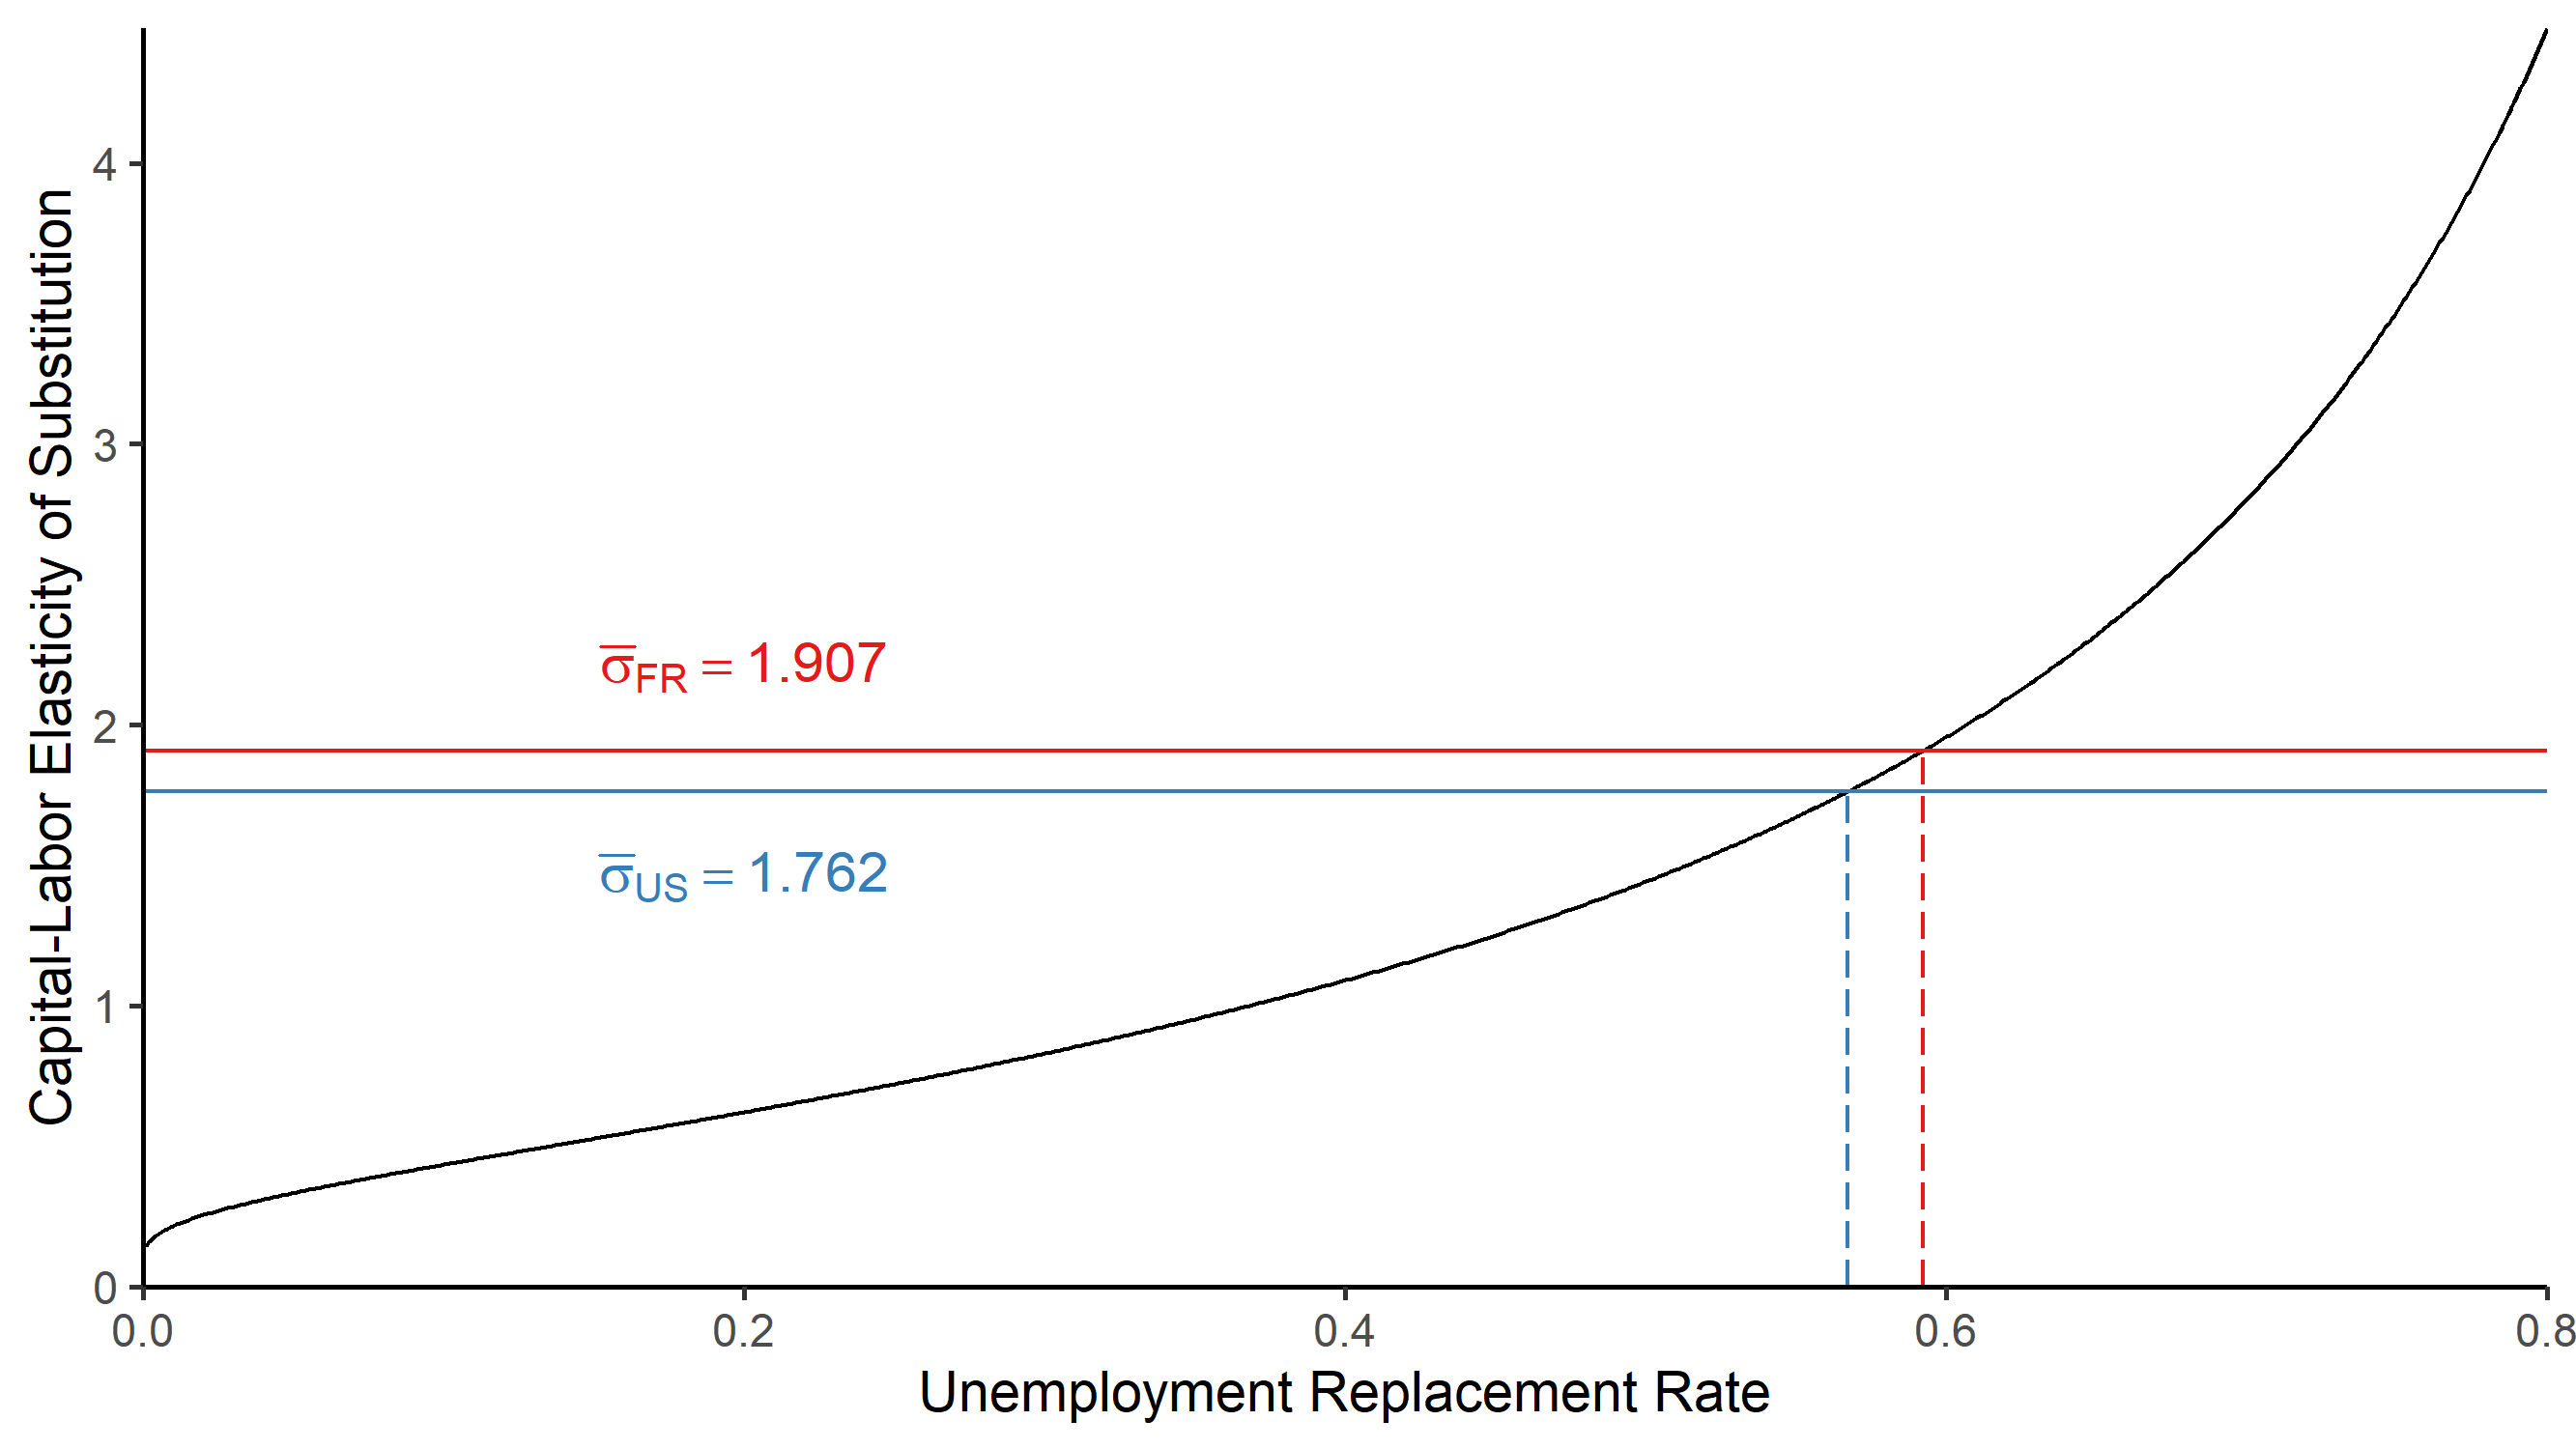
\includegraphics[width = 1\linewidth]{../result/xsigma.png}
%		\vspace{.5ex}
%		\hrule
		\vspace{-6ex}
		\justify\singlespacing\footnotesize The values of $x_{\text{FR}}$ and $x_{\text{US}}$ correspond to the lowest unemployment replacement rate over the period 1970-2010 in France and the United-States for a single-type household specification. Unemployment replacement rate data are from the \href{http://cwed2.org/}{Comparative Welfare Entitlements Dataset 2 (CWED 2)}, see \cite{CWED2017} for more details.
	\end{figure}
% The greater is the unemployment replacement rate, the smaller is the value-added to have a job (i.e. $X_t$).
%All comparative statics are derived in \textbf{Appendix}.

The comparative statics with respect to $X_t$ are as follows
	\begin{equation*}
	\left\lbrace \frac{\partial k_t}{\partial X_t} \gtrless 0 \Rightarrow 
	\left\lbrace \frac{\partial w_t}{\partial X_t} \gtrless 0,~~
	\frac{\partial (Y_t/L_t)}{\partial X_t} \gtrless 0,~~ \frac{\partial w_t}{\partial X_t} <
	\frac{\partial (Y_t/L_t)}{\partial X_t} \right\rbrace \Rightarrow 
	\frac{\partial \theta_t}{\partial X_t} < 0
	\right\rbrace, ~~ \sigma \gtrless 1
	\end{equation*}
When the unemployment replacement rate $\frac{b_t}{(1-\tau_t)w_t}$ increases, the value-added of having a job $X_t$ falls. Hence, the labor share $\theta_t$ increases. The intuition is that when the unemployment replacement rate increases it allows the union to bargain a higher wage and so to grab a relatively larger share of income. This mechanism holds whatever the value of the capital-labor elasticity of substitution $\sigma$. 
% This is an interesting result in the sense that usually CES production functions give rise to results with a threshold on the value of $\sigma$ with respect to unity. 
However, intermediate partial derivatives are just transitional and consider only the partial effect of a change in the unemployment replacement rate.
% Due to the endogeneity of $w_t$, I save the mechanisms analysis for later. 

% Let us focus on the case where capital and labor are gross substitute (i.e. $\sigma>1$). The higher is the unemployment replacement rate, the stronger is the outside option of the representative union which increases the bargained wage with the firm. When the capital and labor are gross substitute (i.e. $\sigma>1$), the firm will compensate the increase in wage by using more capital than labor. Since the representative firm is always on its labor demand curve, \textit{other things equal}, it reduces the labor demand and therefore labor input. Reducing the labor input does shrink the production level of the representative firm. As a result, the labor income share decreases.

\subsection{Equilibrium}\label{equilibrium}

Voting and wage bargaining take place simultaneously and there is no-coordination between the two. As a consequence, both processes take the outcome of the other as given. The interaction determines the equilibrium of the economy. Expressing equations \eqref{eq:inverse_replacement_rate} and \eqref{eq:k(x)} as function of the capital-labor ratio. We have that equilibrium is given by the solution to the following system:
	\begin{align}
		\label{eq:Xg} 
		X_t &= \ln\left( \frac{ \frac{N_t^y}{K_t} k_t - 1 } { \frac{\phi}{1-\phi} k_t^{\frac{\sigma-1}{\sigma}} \eta_t - 1 }\right), \\
		\label{eq:Xh}
		X_t &= \left( \sigma + \frac{1-\phi}{\phi} \frac{1-\gamma(1-\sigma)}{\gamma} k_t^{\frac{1-\sigma}{\sigma}} \right)^{-1},
	\end{align}
which yields the equilibrium capital-labor ratio and employment value-added. Note that at time $t$, the aggregate capital stock $K_t$ is predetermined by the saving decisions at $t-1$, so that $k_t$ is given by $L_t$.

The Cobb-Douglas case, i.e. $\sigma = 1$, can be solved analytically and leads to the following equilibrium:
	\begin{align*}
		X_t &= \frac{\gamma}{1-\phi(1-\gamma)} \\
		k_t &= \left[1 + e^{X_t}\left(\frac{\phi}{1-\phi}\eta_t-1\right)\right]\frac{K_t}{N_t^y}
	\end{align*}
The value-added to have a job is constant, while the capital-per-worker is determined by demographic variables and is proportional to the capital-per-young individual. However, this case is not useful to examine the labor share's dynamics as the labor share is constant with a Cobb-Douglas technology ($\theta_t = 1-\phi$).

In \hyperref[appendix:uniqueness]{appendix A}, I show that the equilibrium is unique for any other value of sigma. The equilibrium is characterized by 13 equations,
	\begin{align}
		\eta_t &= \frac{n_t}{p_t}\frac{1+\alpha p_{t+1}}{\omega}, \tag{Pub. $\eta$} \\
		X_t &= \ln\left( \frac{ \frac{N_t^y}{K_t} k_t - 1 } { \frac{\phi}{1-\phi} k_t^{\frac{\sigma-1}{\sigma}} \eta_t - 1 }\right), \label{eq:g}\tag{Eq. $g$} \\
		X_t &= \left( \sigma + \frac{1-\phi}{\phi} \frac{1-\gamma(1-\sigma)}{\gamma} k_t^{\frac{1-\sigma}{\sigma}} \right)^{-1}, \label{eq:h}\tag{Eq. $h$}\\
		L_t &= \frac{K_t}{k_t}, \tag{Prod. $L$} \\
		w_t &= A(1-\phi)\left( \phi k_t^\frac{\sigma-1}{\sigma} + 1-\phi \right)^\frac{1}{\sigma-1}, \tag{Prod. $w$}\\
		Y_t &= A \left[ \phi K_t^\frac{\sigma-1}{\sigma} + (1-\phi) L_t^\frac{\sigma-1}{\sigma} \right]^\frac{\sigma}{\sigma-1}, \tag{Prod. $Y$}\\
		u_t &= 1 - \frac{L_t}{N_t^y}, \tag{Prod. $u$}\\
		\theta_t &= \left(1 + \frac{\phi}{1-\phi} k_t^\frac{\sigma-1}{\sigma} \right)^{-1}, \tag{Prod. $\theta$} \\
		\tau_t &= 1 - \left[ (1-\theta_t)(1+\beta+\eta_t) \right]^{-1}, \tag{Pub. $\tau$}\\
		b_t &= (1-\tau_t) w_t e^{-X_t}, \tag{Pub. $b$}\\
		h_t &= \frac{\tau_t Y_t - b_t u_t N_t^y}{N_t^o}, \tag{Pub. $h$}\\
		S_t &= \frac{\alpha p_{t+1}}{1 + \alpha p_{t+1}} \left[ (1-\tau_t)w_t(1-u_t) + b_tu_t \right] N_t^y, \tag{HH. $S$}  \\
		K_{t+1} &= S_t.	\tag{HH. $K$}
	\end{align}
Let define, respectively, equations \eqref{eq:g} and \eqref{eq:h} with the functions $g(L_t, K_t, \eta_t, N_t^y; \phi, \sigma)$ and $h(L_t, K_t; \sigma, \phi, \gamma)$, such that:
	\begin{align*}
		X_t &= g(L_t, K_t, \eta_t, N_t^y; \phi, \sigma) 
		%&= \ln\left[ \frac{ \frac{N_t^y}{L_t} - 1 } { \frac{\phi}{1-\phi} \left(\frac{K_t}{L_t}\right)^{\frac{\sigma-1}{\sigma}} \eta_t - 1 }\right]
		\\
		X_t &= h(L_t, K_t; \sigma, \phi, \gamma) 
		%&= \left[ \sigma + \frac{1-\phi}{\phi} \frac{1-\gamma(1-\sigma)}{\gamma} \left(\frac{K_t}{L_t}\right)^{\frac{1-\sigma}{\sigma}} \right]^{-1}
	\end{align*}
Differentiating this system, I find that
	\begin{align*}
		dX_t &= g_L dL_t + g_K dK_t + g_\eta d\eta_t + g_{N^y} dN_t^y, \\
		dX_t &= h_L dL_t + h_K dK_t,
	\end{align*}
where $f_x$ is the partial derivative of $f$ with respect to $x$. Solving the system, I have
	\begin{equation*}
		dL_t = \frac{1}{h_L-g_L}\left[(g_K-h_K) dK_t + g_\eta d\eta_t + g_{N^y} dN_t^y \right]
	\end{equation*}
The variables $\eta_t$ and $N_t^y$ are given by the demographic dynamics while the capital stock $K_t$ is given by savings of the previous period. Thus, the variable that determines the equilibrium is the level of employment $L_t$. Partial derivatives are derived in \hyperref[appendix:derivatives]{appendix B}. $g_\eta$ is negative because the greater is the youth's political power, the greater is the unemployment benefit and the smaller is the value-added to have a job. $g_{N^y}$ is positive because the more numerous the young are, the more these unemployment benefits are divided among them and so the smaller is the value-added to have a job. The sign of $g_K-h_K$ depends on the value of $\sigma$ with $g_K-h_K \lessgtr 0, ~ \forall \sigma \gtrless 1$. This is directly related to the fact that both factors are either gross substitutes or gross complements. When labor and capital are gross substitutes, more capital requires less labor for a given of level of output, while when they are complements, the representative firm has to jointly increase labor and capital stock in order to maintain the same production level. Lastly, the sign of $h_L-g_L$ is ambiguous. When $\sigma < 1$, then $g_L$ and $h_L$ are both positive, thus, $g_L-h_L$ is ambiguous. When $\sigma > 1$, $h_L$ is unambiguously negative. The sign of $g_L$ cannot be determined without additional assumptions. If $\eta_t/\Theta_t > \sigma$, then $g_L$ is negative. Otherwise, $g_L$ is negative if the unemployment rate is lower than a certain threshold, i.e $u_t < \bar{u}_t$ where $\bar{u}_t = \left(2 - \frac{\eta_t}{\Theta_t\sigma}\right)^{-1}$. Thus, when the unemployment rate is high enough such that $u_t > \bar{u_t}$, $g_L$ is unambiguously positive and so is $g_L-h_L$. This is the only case where it is possible to determine unambiguously the impact of variables on $L_t$. In such a case, $\frac{dL_t}{dK_t}\Bigr|{\substack{d\eta_t = 0\\dN_t^y = 0}} < 0$, $\frac{dL_t}{dN^y_t}\Bigr|{\substack{dK_t = 0\\d\eta_t = 0}} > 0$ and $\frac{dL_t}{d\eta_t}\Bigr|{\substack{dK_t = 0\\dN_t^y = 0}} < 0$. Therefore, except in this special case, $g_L-h_L$ is ambiguous. Due to the ambiguity of $g_L$, I perform a quantitative analysis in section \ref{sec:quantitative_analysis}.
	
	\section{Quantitative analysis} \label{sec:quantitative_analysis}
	% !TeX spellcheck = en_US
There are three objectives in this quantitative analysis. Firstly, to match the labor share dynamics over the period 1970 to 2010. Secondly, to produce model predictions over the period 2010 to 2080. Finally, to decompose demographic effects on the labor share and their transmission channels. Based on analytical results, I compute quantitative predictions for France and the United-States. One period in the model corresponds to 40 years in the data. Following the methodology of \cite{Gonzalez-Eiras2012} to simulate an OLG model, I compute four sequences of model predictions with a period length of 40 years each. Periods of the first sequence corresponds to 1970, 2010, 2050, ... ; for the second sequence to 1980, 2020, 2060, ... ; for the third sequence to 1990, 2030, 2070, ... ; for the fourth sequence to 2000, 2040, 2080, ... . When reporting time series predictions, I list the four sequences in a single time series.

\subsection{Calibration}\label{subsec:calibration}
With a period length of 40 years, agents are considered as young between their 20 to 60 years old and as elderly thereafter.\footnote{An implicit assumption of the model is that retirement age is constant (this assumption is discussed in section \ref{sec:discussion}). The french average effective retirement age is about 67.8 years-old in 1970 and has declined down to 59.3 in 2010. While the US one has moved from 68.4 to 65.6 over the same period (data from the \href{https://www.oecd.org/els/emp/average-effective-age-of-retirement.htm}{OECD Database}). I suppose, as an approximation, that agents retire at 60 years-old to match period lengths of the calibration. Such an assumption should not affect the voting outcome because almost-retired agents may anticipate their future situation once they vote. However, implications in terms of labor supply might be discussed. Nonetheless, 5 years approximation remains marginal compared to the 40 years between two periods. %\textbf{Justification/Argument to improve.}
} I compute the old-age dependency ratio from the data as the number of old households divided by the number of young households (i.e. $p_t/n_t \equiv N_t^o/N_t^y$). Then, the population growth rate at time $t$ is computed using the ratio between the number of young households in period $t$ relative to the number of young households in the previous period of the sequence (i.e. $n_t = N_t^y/N_{t-1}^y$). Finally, the survival rate at time $t$ is the product of the old-age-dependency ratio and the population growth.%(i.e. $p_t = \psi_t n_t$).
\footnote{Demographic data from 1950 are taken from the \href{https://population.un.org/wpp/}{United Nations World Population Prospects 2017}. Demographic data before 1950 are from \href{http://www.populstat.info}{http://www.populstat.info}. Demographic data between 2010 and 2100 are the ``medium variant'' estimates from the United Nations. Both rates $n_t$ and $p_t$ converges to unity in the very long run (after the 5th period of the 4th sequence, hence 2160). However, I limit my analysis to 3 periods (hence 2080) due to high uncertainty above 100 years.} Figure \ref{fig:demo} plots demographic variables for both countries.

\begin{figure}[tb]
	\centering
	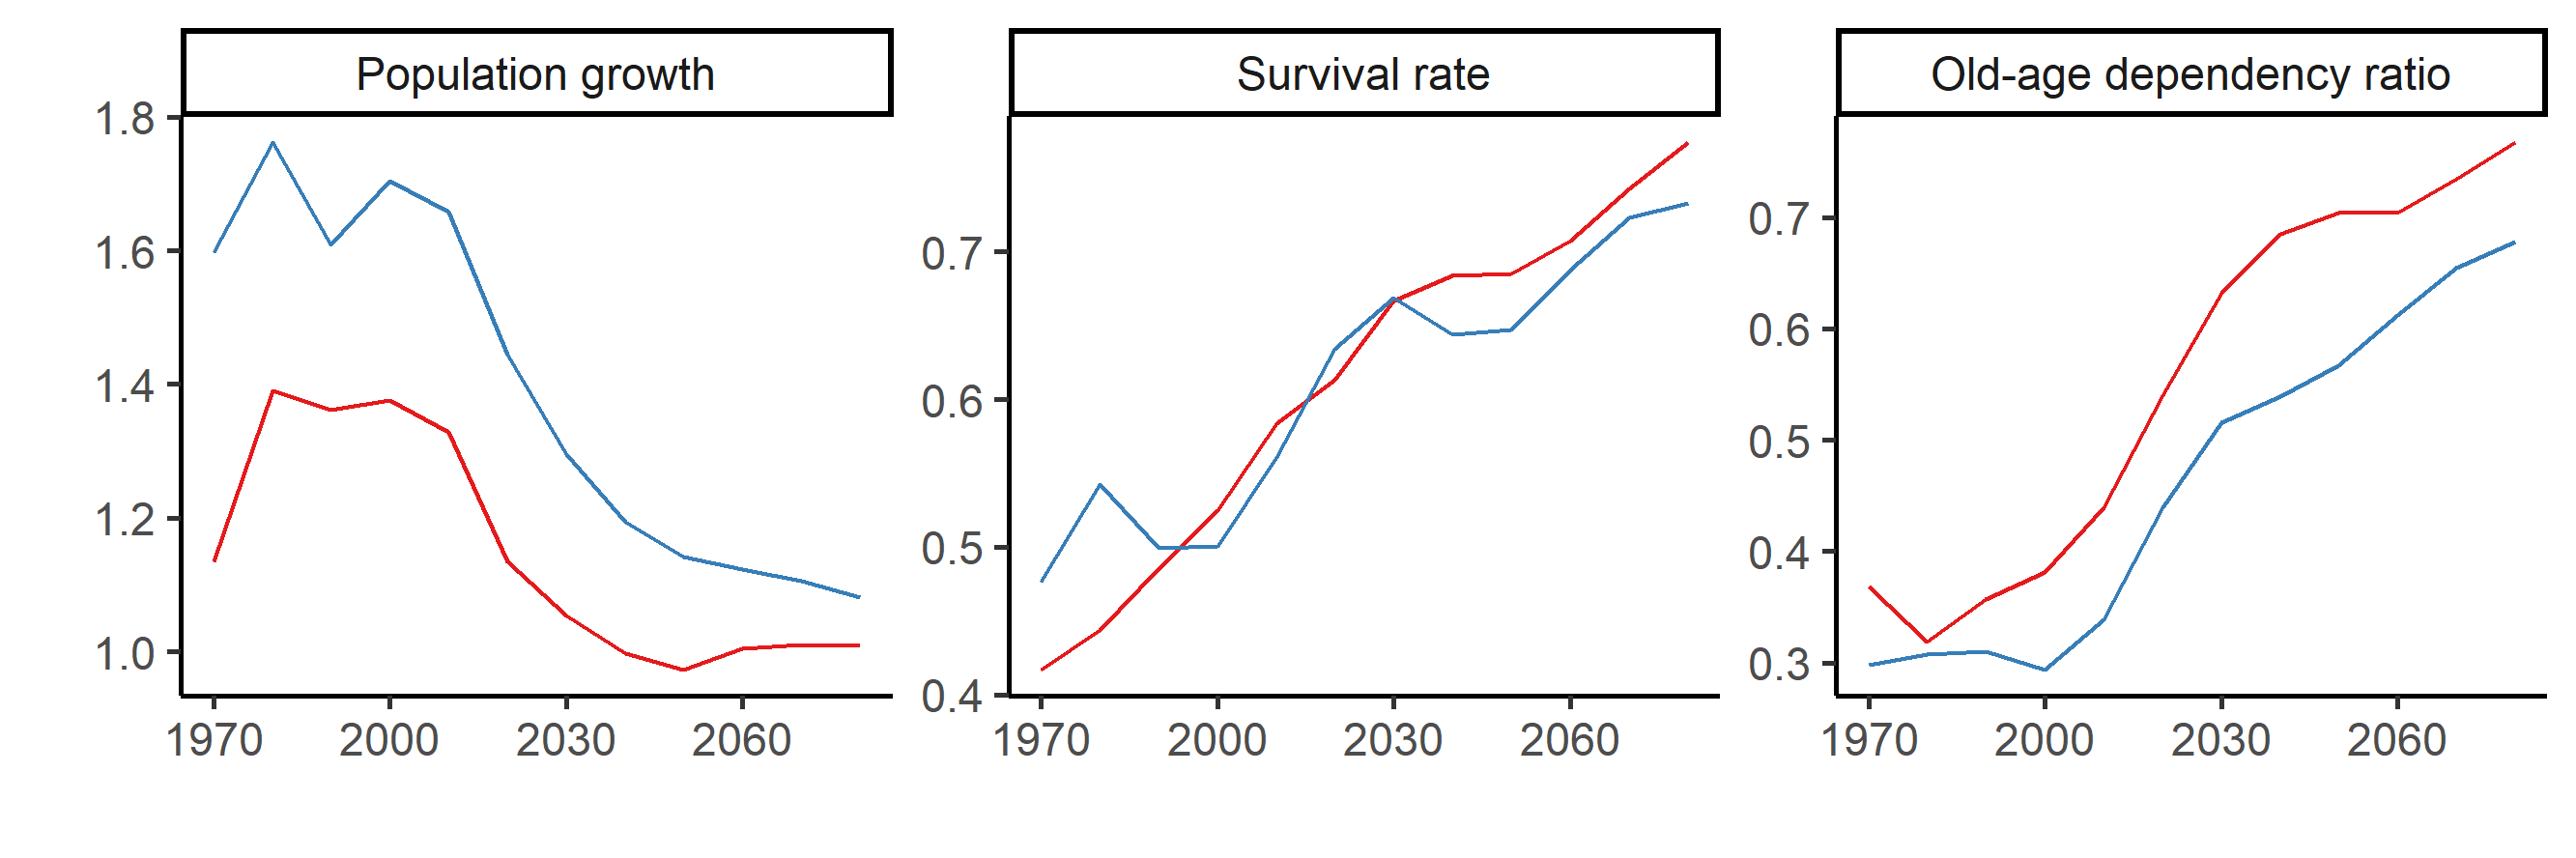
\includegraphics[width=\linewidth]{../result/demo_npdep.png} 
	\caption{Demographic variables time series}\label{fig:demo}
	\vspace{.5ex}
	\hrule
	\vspace{-4ex}
	\justify\singlespacing\footnotesize \textit{Notes:} The black curves refer to France and the gray ones to the United-States.
\end{figure}

%% Normalization %%
Economic variables data ($K_t$, $emp_t$, $Y_t$, $\theta_t$) are taken from the \href{https://www.rug.nl/ggdc/productivity/pwt/}{Penn World Table 9.1}.\footnote{$K$ is the capital stock at constant 2011 national prices, $emp$ the number of persons engaged, $Y$ the real GDP at constant 2011 national prices and $\theta$ the share of labor compensation in GDP. $K$ and $Y$ are adjusted with the average annual hours worked by persons engaged. For further details the reader is referred to \cite{Feenstra2015}.} 
When considering data on the labor share, \cite{Gollin2002} shows that it is necessary to take into account self-employed income. In the model, workers are only young individuals and provide only labor supply. Therefore, I assume that self-employed people earn an income that is characterized as a compensation.\footnote{This specification corresponds to the first adjustment method of \cite{Feenstra2015}.}
I also use the government revenue in \% of GDP from the \href{https://data.oecd.org/tax/tax-revenue.htm}{OECD database} as proxy for the tax rate $\tau_t$.
% Unemployment and redistribution
In the model, labor supply is inelastic and there is no distinction between unemployed and inactive households. Unemployed agents in terms of the model specification corresponds to all agents that do not work. However, in high-income countries, such as France and United States, inactive individuals also benefits from redistribution. This redistribution is captured through unemployment benefits $b_t$ in the model.
I compute the unemployment rate such that $u_t = 1 - emp_t/N^{15-64}_t$, where $N_t^{15-64}$ is the working age population.\footnote{I consider the whole working age population instead of the young population in order to compute the unemployment rate. Due to demographic specification of the model, young agents correspond to those between 20 and 60 years old. The number of persons engaged ($emp$) per age groups are not available in \href{https://www.rug.nl/ggdc/productivity/pwt/}{PWT 9.1}. Therefore, taking only $N^y_t$ as denominator would bias downward the unemployment rate.} Results are robust to different specifications of the unemployment rate.
%\textbf{details in the Appendix (to be written)}. 
Then, I compute labor such that $L_t=(1-u_t)N_t^y$. I normalize $K_t$ and $L_t$ to their 1970 values. As a consequence, the capital-to-labor ratio $k_t$ is also normalized and is equal to 1 in 1970. Then, $N_t^y$ and $N_t^o$ are normalized such that $u_t$ matches the data in 1970.

%% sigma estimation %% %% Parameters to calibrate %%
Once all stock variables are normalized, I calibrate the 7 parameters $\lbrace \phi, \sigma, \gamma, \alpha, \omega, \beta, A \rbrace$. Table \ref{tab:param} summarizes parameters for both countries.
% Parameters table
\begin{table}[tb]
	\caption{Parameters}\label{tab:param}
	\centering
	\begin{threeparttable}
		\begin{tabular}{c l D{.}{.}{-3} D{.}{.}{-3}}
			\multicolumn{2}{c}{\textbf{Parameter}} & \multicolumn{1}{r}{\textbf{France}} & \multicolumn{1}{r}{\textbf{United States}}            \\ \hline \hline
			$\phi$             & Capital share in 1970                           & 0.27 & 0.325		\\ \hline
			$\gamma$           & Relative bargaining power of the union          & 0.5 & 0.5				\\ [-1ex]
			$\alpha$           & Discount rate                                   & 0.669 & 0.669		\\ \hline
			$\sigma$           & Capital-labor elasticity of substitution        & 1.279 & 1.234	\\ \hline
			$\omega$           & Relative ideological spread-out				 & 0.983 & 1.533		\\ [-1ex]
			$\beta$            & Preference for government health expenditure    & 0.739 & 0.138		\\ [-1ex]
			$A$                & Scale parameter of the production function		 & 28.23 & 22.84				\\ \hline \hline
		\end{tabular}
		\vspace{-3ex}
		\begin{tablenotes}
			{\singlespacing\footnotesize
				\item \textit{Note :} Single-equation estimation of $\sigma$ from the two first-order conditions of the profit maximization with normalized CES production function. $\sigma$ estimates are significant at $p<0.1$ for France and $p<0.05$ for the United States. Details in \hyperref[appendix:sigma]{appendix C}.
			}
		\end{tablenotes}
	\end{threeparttable}
\end{table}
The first parameter $\phi$ corresponds to the capital share in 1970. Because the capital-to-labor ratio is normalized (i.e. $k_{1970} = 1$), the labor share $\theta$ in 1970 is equal to $1-\phi$. The main parameter of the model is the elasticity of substitution between capital and labor $\sigma$. I estimate it using a combination of the first order conditions of the profit maximization. Details of the estimation in \hyperref[appendix:sigma]{appendix C}. I obtain 1.279 and 1.234, respectively, for France and the United States. According to the estimation, both input factors are gross substitute. These estimates are in line with \cite{Karabarbounis2014} who use cross-sectional data on 50 countries over the period 1975-2012 to find an elasticity greater than 1 and on average around 1.28 in their baseline estimates. I set the relative bargaining power of the union $\gamma$ to 0.5. Hence, I assume that neither the representative union nor the representative firm have any other advantage in the bargaining apart from their respective outside options. I also set the discount rate at 0.669 according to the literature. Then, I have three remaining parameters that are deduced. The relative ideological spread-out $\omega$ is set such that the model prediction matches the capital-to-labor ratio $k$ in 1970. The preference for government health expenditure $\beta$ is set to match the tax rate $\tau$ in 1970. Finally, the scale parameter of the production function $A$ is set with grid-search to match the average labor share between 2008 and 2012.

Due to initial labor share values, the parameter distribution $\phi$ which correspond to the capital share in 1970 is larger in the United States than in France. Moreover, the relative per-capita political influence of old households $\omega$ is also greater. This deduced parameter suggests that young generations have less political weight in the United States compared to France. Notice that $\omega$ is lower than one for France. It implies that French youth voting behavior is more sensitive to policy changes compared to elderly. French households have a much greater preference for government health expenditure $\beta$. Finally, the scale parameter $A$ is ranged between 20 and 30 for both countries.

\subsection{Model predictions over the period 1970-2010}\label{subsec:model_pred}

\subsubsection{The labor share decline}

Figure \ref{fig:baseline7010} displays the labor share from model predictions and data over the period 1970-2010.
\begin{figure}[tb]
	\centering
	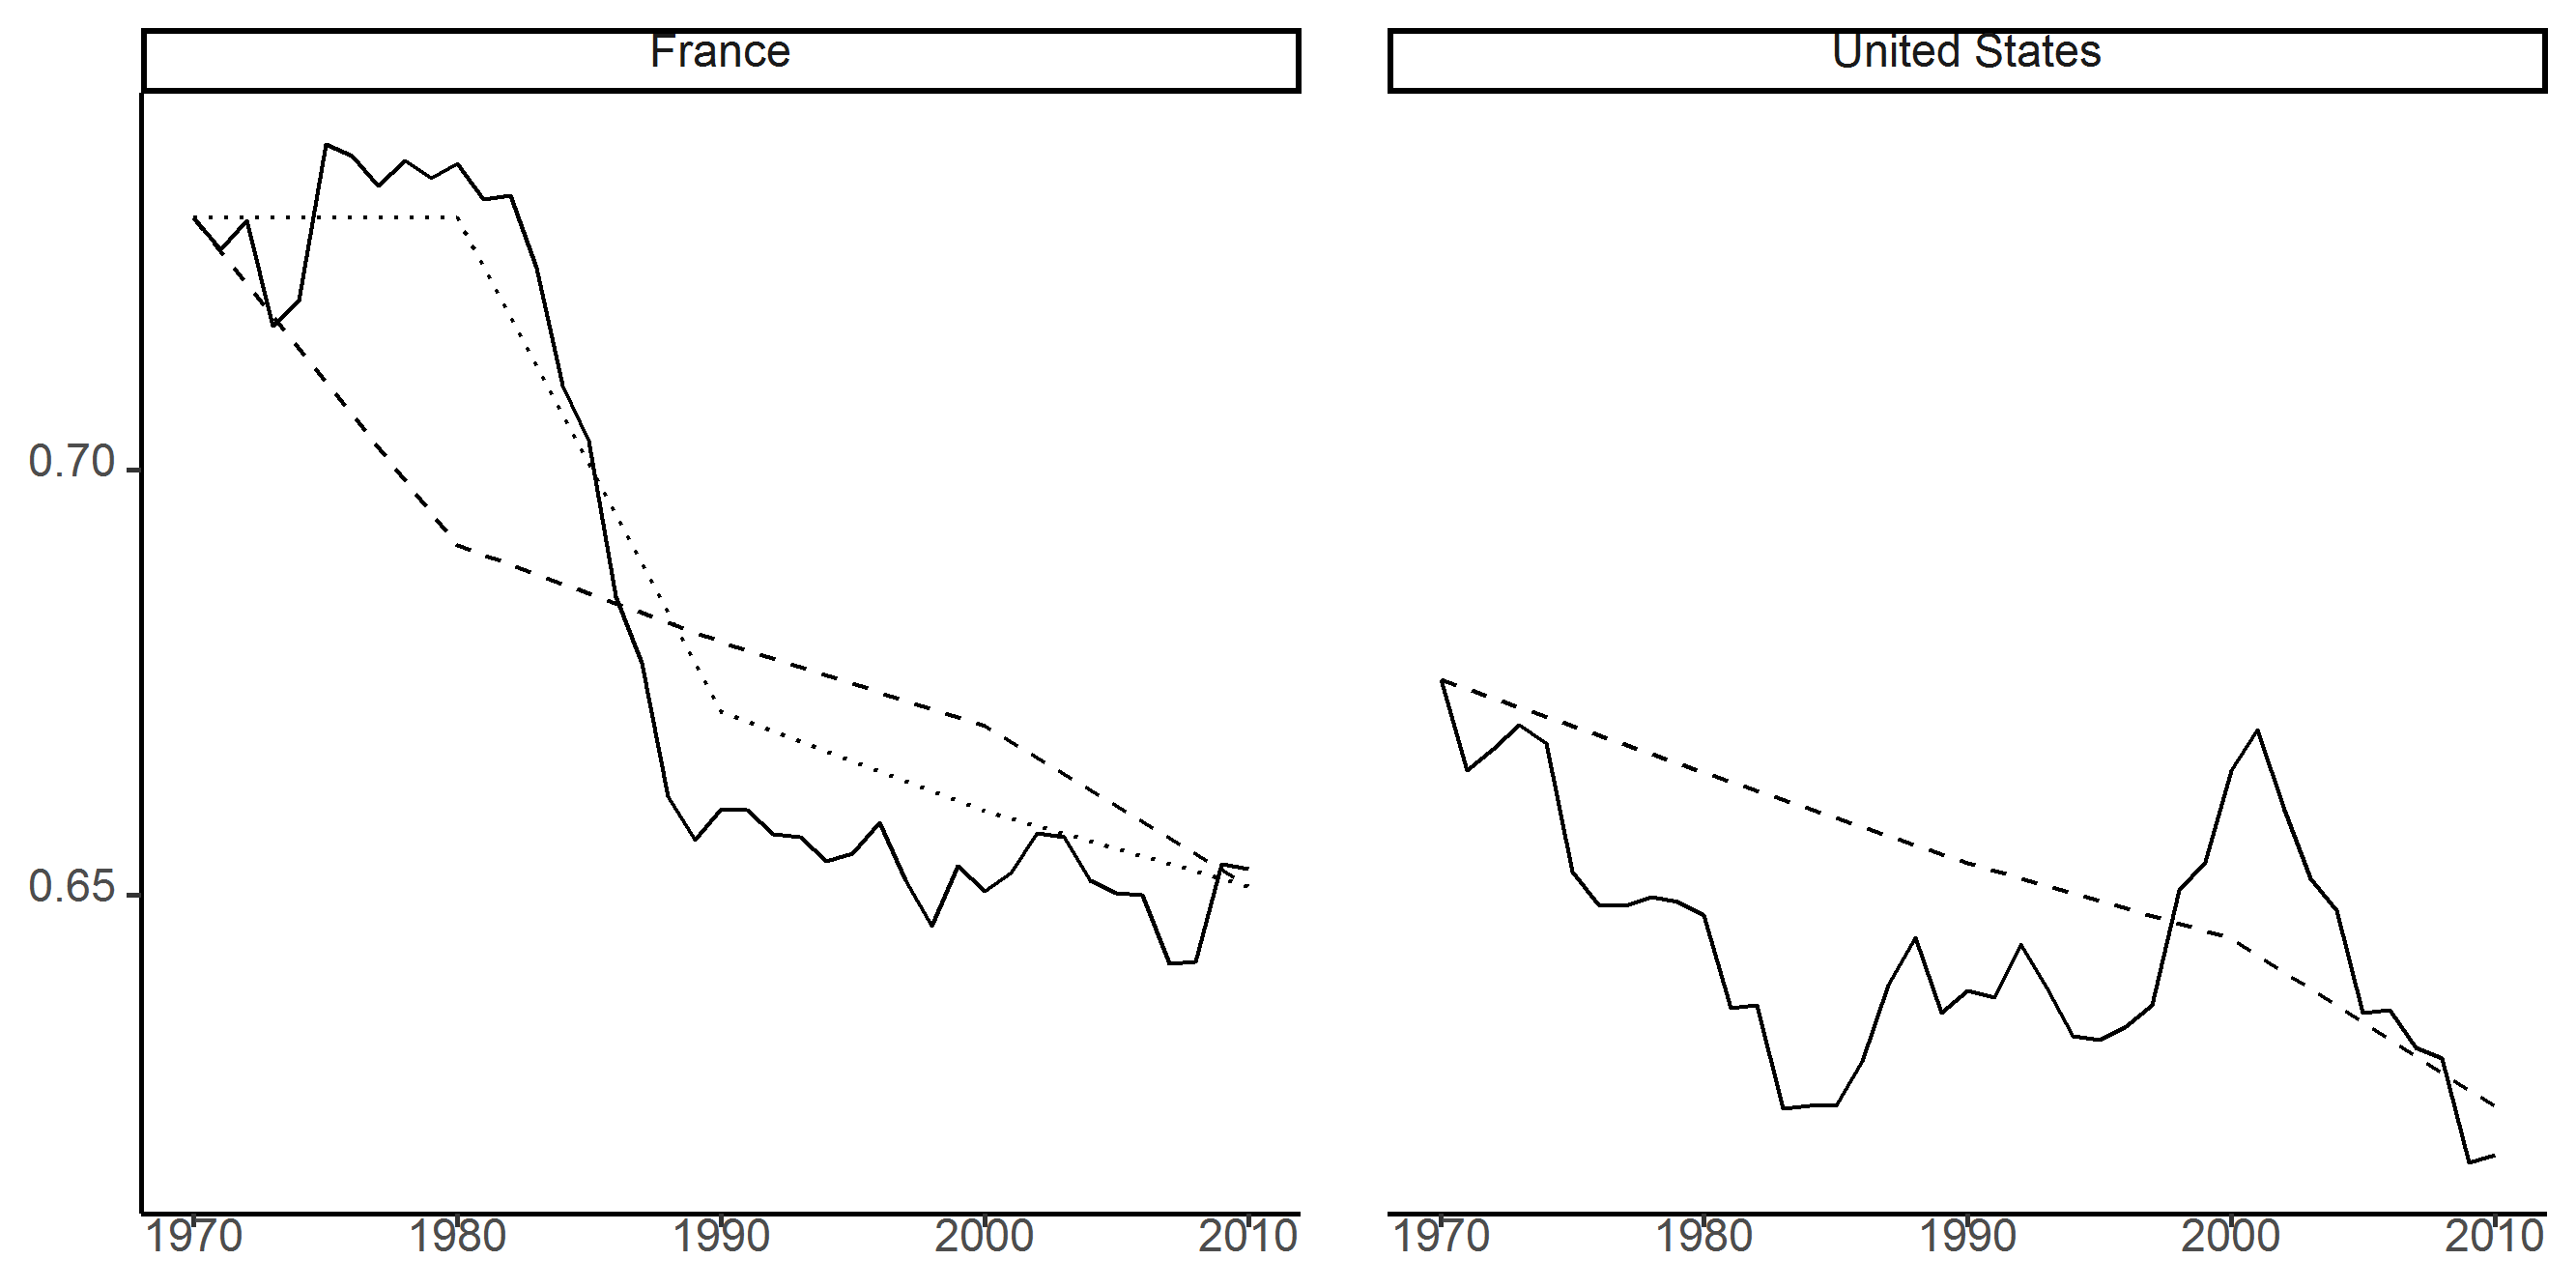
\includegraphics[width=1\linewidth]{../result/baseline7010.png}
	\caption{Model prediction of the labor share}
	\label{fig:baseline7010}
	\vspace{.5ex}
	\hrule
	\vspace{-4ex}
	\justify\singlespacing\footnotesize \textit{Notes:} The solid curve corresponds to the labor share in the data, from the \href{https://www.rug.nl/ggdc/productivity/pwt/}{Penn World Table 9.1} with adjustment method 1. The dashed curve is the model prediction with a unique capital-labor elasticity of substitution. The dotted curve is the model prediction for France with a break in the regime for the capital-labor elasticity of substitution (details in \hyperref[appendix:regime]{appendix D}).
\end{figure}
The model reproduces the global trend of the data for both countries. For France, the model is not able to reproduce the huge decline of the labor share between 1980 and 1990. This gap may be explained by different factors not considered in the model.
%% Firing cost : Bentolila and Bertola
I modelize the workers outside option within the wage bargaining using only unemployment benefits and the tax rate. Other labor market institutions may have played a role in firms' employment policies during this period. Indeed, I consider a right-to-manage specification, meaning that the firm has the prerogative to hire and fire. In my framework, there is no firing cost. \cite{Bentolila1990} build a model with linear adjustment cost and find that firing costs have an effect on firms propensity to hire and fire. Further, they also find that firing costs slightly increase average long-run employment. Subsequent to the oil shock, firms were not able to fire as they would have due to high firing costs.\footnote{\cite{Blanchard1997} also shows that wages failed to adjust to the productivity slowdown and adverse supply shocks of the 1970s. Thus, wages remained relatively high and so did the labor share. This phenomenon was more pronounced in European Continental countries than in the Anglo-Saxon countries, mainly due to labor market institutions.} They reduced employment with attrition, thus the process took time and the employment remained higher than it should during some years. In addition, most of the employment security policies were introduced between the 1960s and the beginning of the 1970s. Here again, these protections may be the result of the baby-boomers generation operating a political pressure to secure employment. Although, I do not integrate it in the model. Then, France during the 1980s has started to implement policies in order to make the labor market more flexible. For instance, short term contracts have been introduced in 1979. To summarize, the labor market institutions in France were tremendously different before and after the 1980s. The reason why the model prediction does not reproduce the labor share from the data owes to the calibration of the model that is in line with the labor market institutions after 1980, but not before. Another way to think about it, in terms of the model, is to suppose that the capital-labor elasticity of substitution was much smaller before 1980.\footnote{Perhaps even lower than 1, meaning that an increase in $k_t$ leads to an increase in $\theta_t$.} Therefore, the representative firm was constrained and not able to substitute labor by capital as much as the model predicts.
%% Other reason ?
%\textbf{Blanchard ? / Outside option ?}.
In line with the above arguments, I investigate whether there is a change in the regime of $\sigma$ over this period. Details of the methodology in \hyperref[appendix:regime]{appendix D}. I find that such a break has occurred during the 1980s in France. The dotted curve is the model prediction with a capital-labor elasticity of substitution of 1 in 1970-1980 and about 1.321 thereafter. The scale parameter $A$ is also changed to 23.891 for France.
For the United States, the model tends to overestimate the labor share in 1980 and 1990 and underestimate it in 2000.
%\textbf{Explanations / References ?}. 
However, model predictions capture the global trend of the labor share over the period.
%% Transition Mechanism analysis
To highlight the mechanisms of this decline, it is necessary to look at the variations of determinant variables.

\subsubsection{Mechanisms of the decline}

The state of the economy is determined by the interaction of the wage bargaining and the voting. Both processes take place simultaneously. The demographic context over this period, as presented in figure \ref{fig:demo}, is such as the population growth $n_t$ slightly exceeds the increasing survival rate $p_t$. Thus, the old-age-dependency $p_t/n_t$ remains relatively constant between 1970 and 2000. With a decline in France in 1980 due to the massive entry of the baby-boomers in the labor force. Finally, the old-age-dependency ratio starts to increase between 2000 and 2010 due to a steady population growth but a sharply increasing survival rate. This increase is also due to the baby-boomers' cohort who begins to retire. As a result of this demographic context, the youth political weight $\eta_t$ was above its 1970's level until 2000 in both countries.

% Public Policy
Figure \ref{fig:dev_public7010} displays the deviation from the 1970 steady-state of public policy variables in percentage.
\begin{figure}[tb]
	\centering
	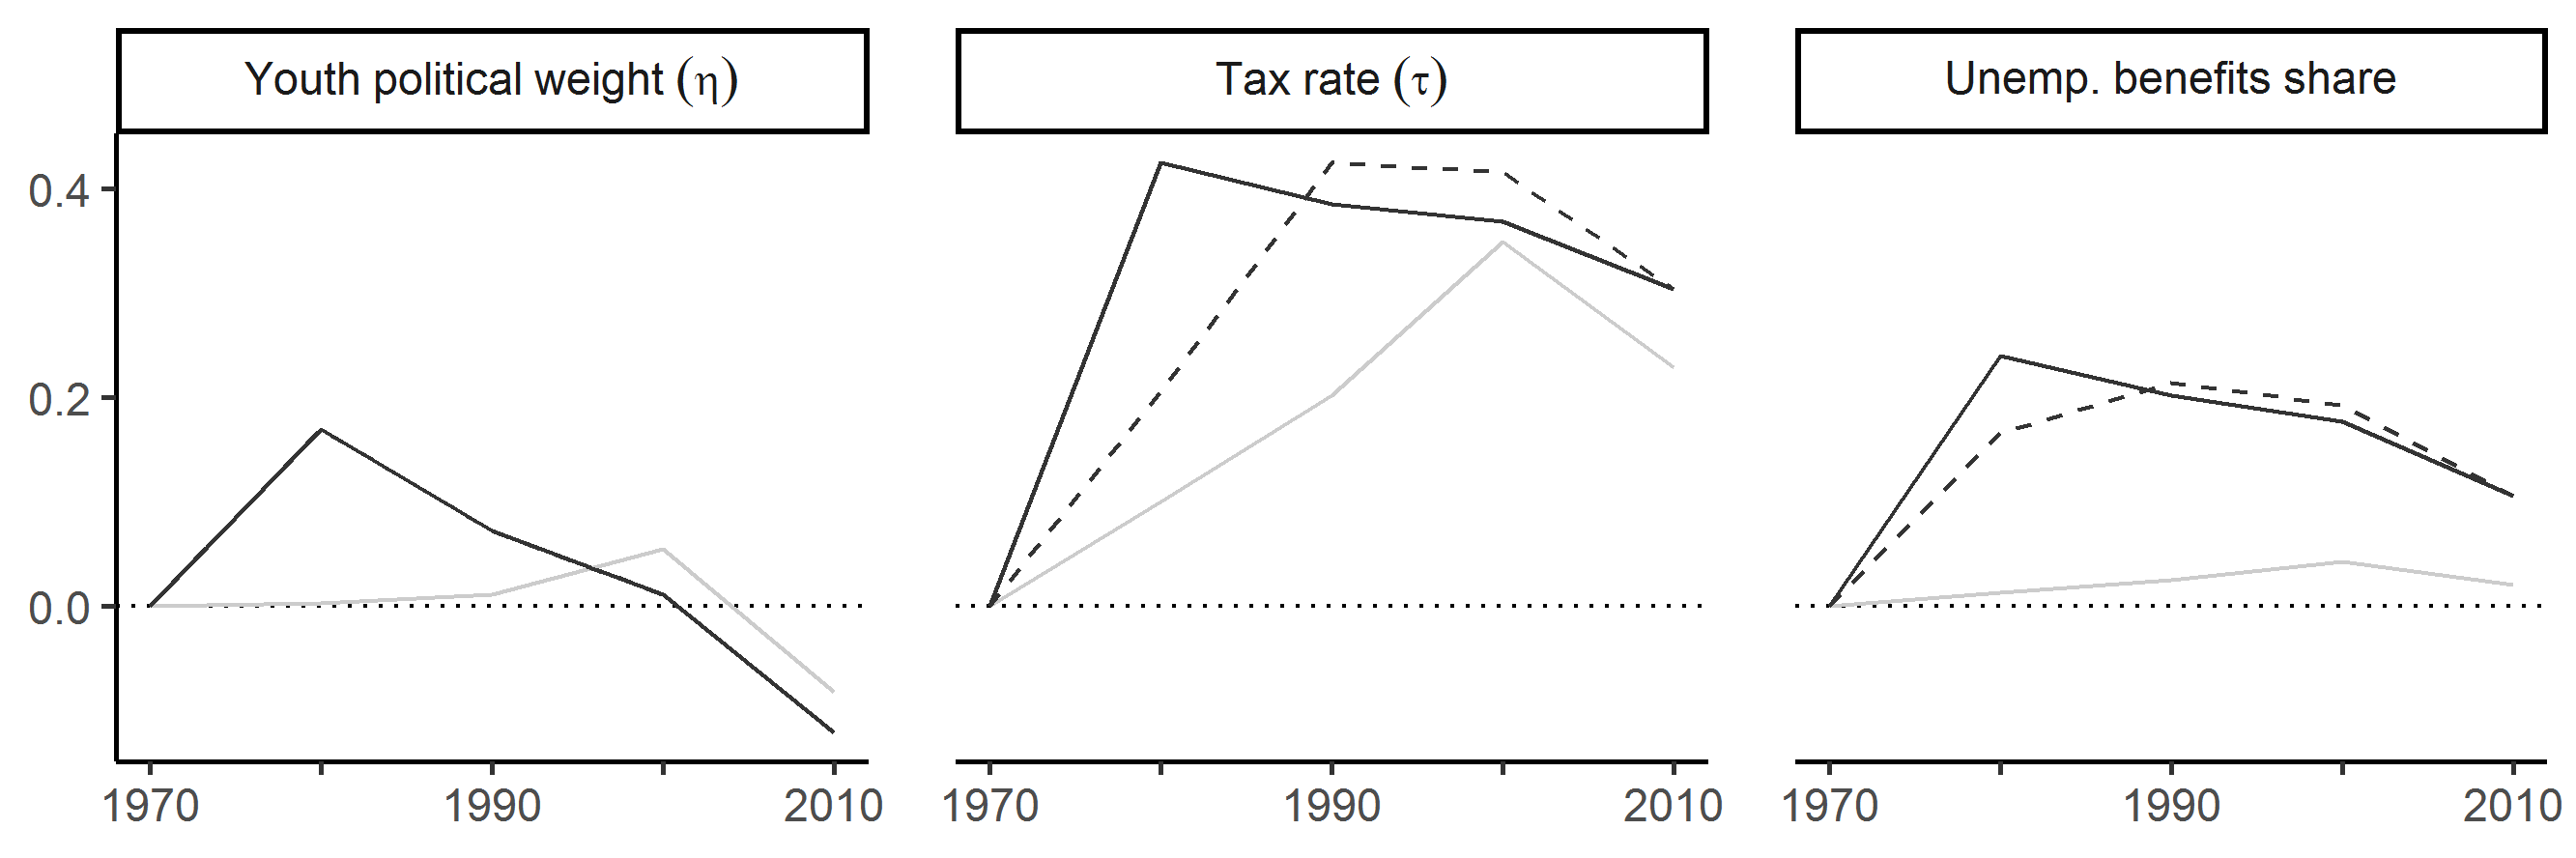
\includegraphics[width=1\linewidth]{../result/deviation/dev_public7010.png}
	\caption{Deviation from the 1970 steady-state of public policy variables}
	\label{fig:dev_public7010}
	\vspace{.5ex}
	\hrule
	\vspace{-4ex}
 	\justify\singlespacing\footnotesize \textit{Notes:} The unemp. benefits share corresponds to the share of the unemployment benefits in the government spending, i.e. $buN^y/(\tau Y)$. The black curves refer to France and the gray ones to the United-States. The solid curves refer to the model predictions with a unique capital-labor elasticity of substitution and the dashed ones to the model prediction for France with a break in the regime for the capital-labor elasticity of substitution.
\end{figure}
As the youth political weight raises and because they desire more redistribution, the tax rate $\tau_t$ increases (i.e. $\partial \tau_t / \partial \eta_t > 0$). Due to the opportunistic behavior of political parties, pro-youth policies are implemented. In the model, pro-youth policies correspond to pro-labor policies and are translated in terms of unemployment benefits in order to insure the unemployment risk. Thus, the unemployment benefits share in government revenue $b~share$ increases at the cost of the government health spending share in government revenue.

% Outside option
%Figure \ref{fig:dev_outside_7010} displays the deviation from the 1970 steady-state of outside option variables in percentage.
%\begin{figure}[!ht]
%	\centering
%	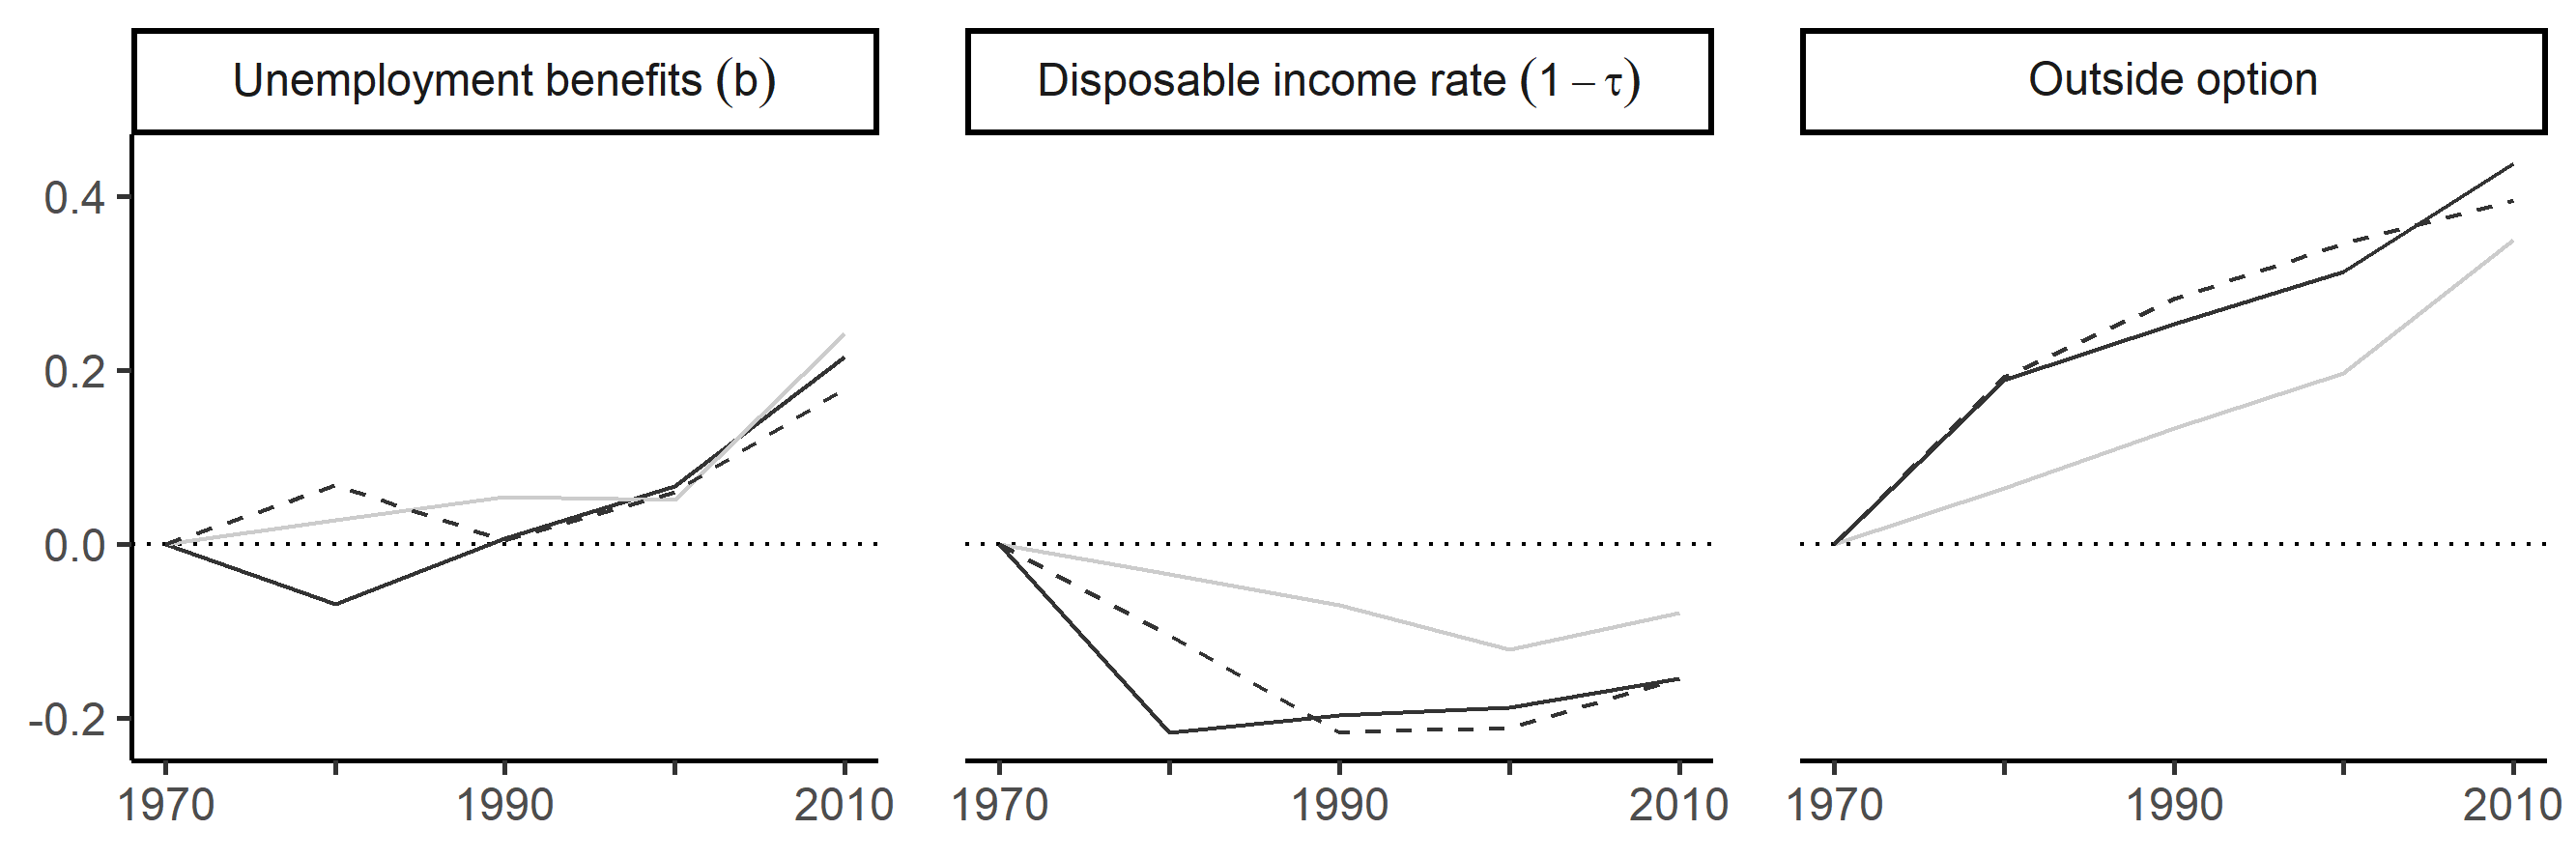
\includegraphics[width=1\linewidth]{../result/deviation/dev_outside7010.png}
%	\caption{Deviation from the 1970 steady-state of outside option variables.}
%	\label{fig:dev_outside_7010}
%	\vspace{.5ex}
%	\hrule
%	\vspace{-4ex}
%	\justify\singlespacing\footnotesize $b$ is the unemployment benefits per capita, $1-\tau$ \textbf{the disposable income rate} and $b/(1-\tau)$ the outside option. The reader is referred to the footnote of the figure \ref{fig:pred_data_7010} for the legend of the curves.
%\end{figure}

% Wage bargaining
These policy changes interact with the wage bargaining because they affect the outside option of the young agents. Figure \ref{fig:dev_bargain7010} displays the deviation from the 1970 steady-state of wage bargaining variables in percentage.
\begin{figure}[tb]
	\centering
	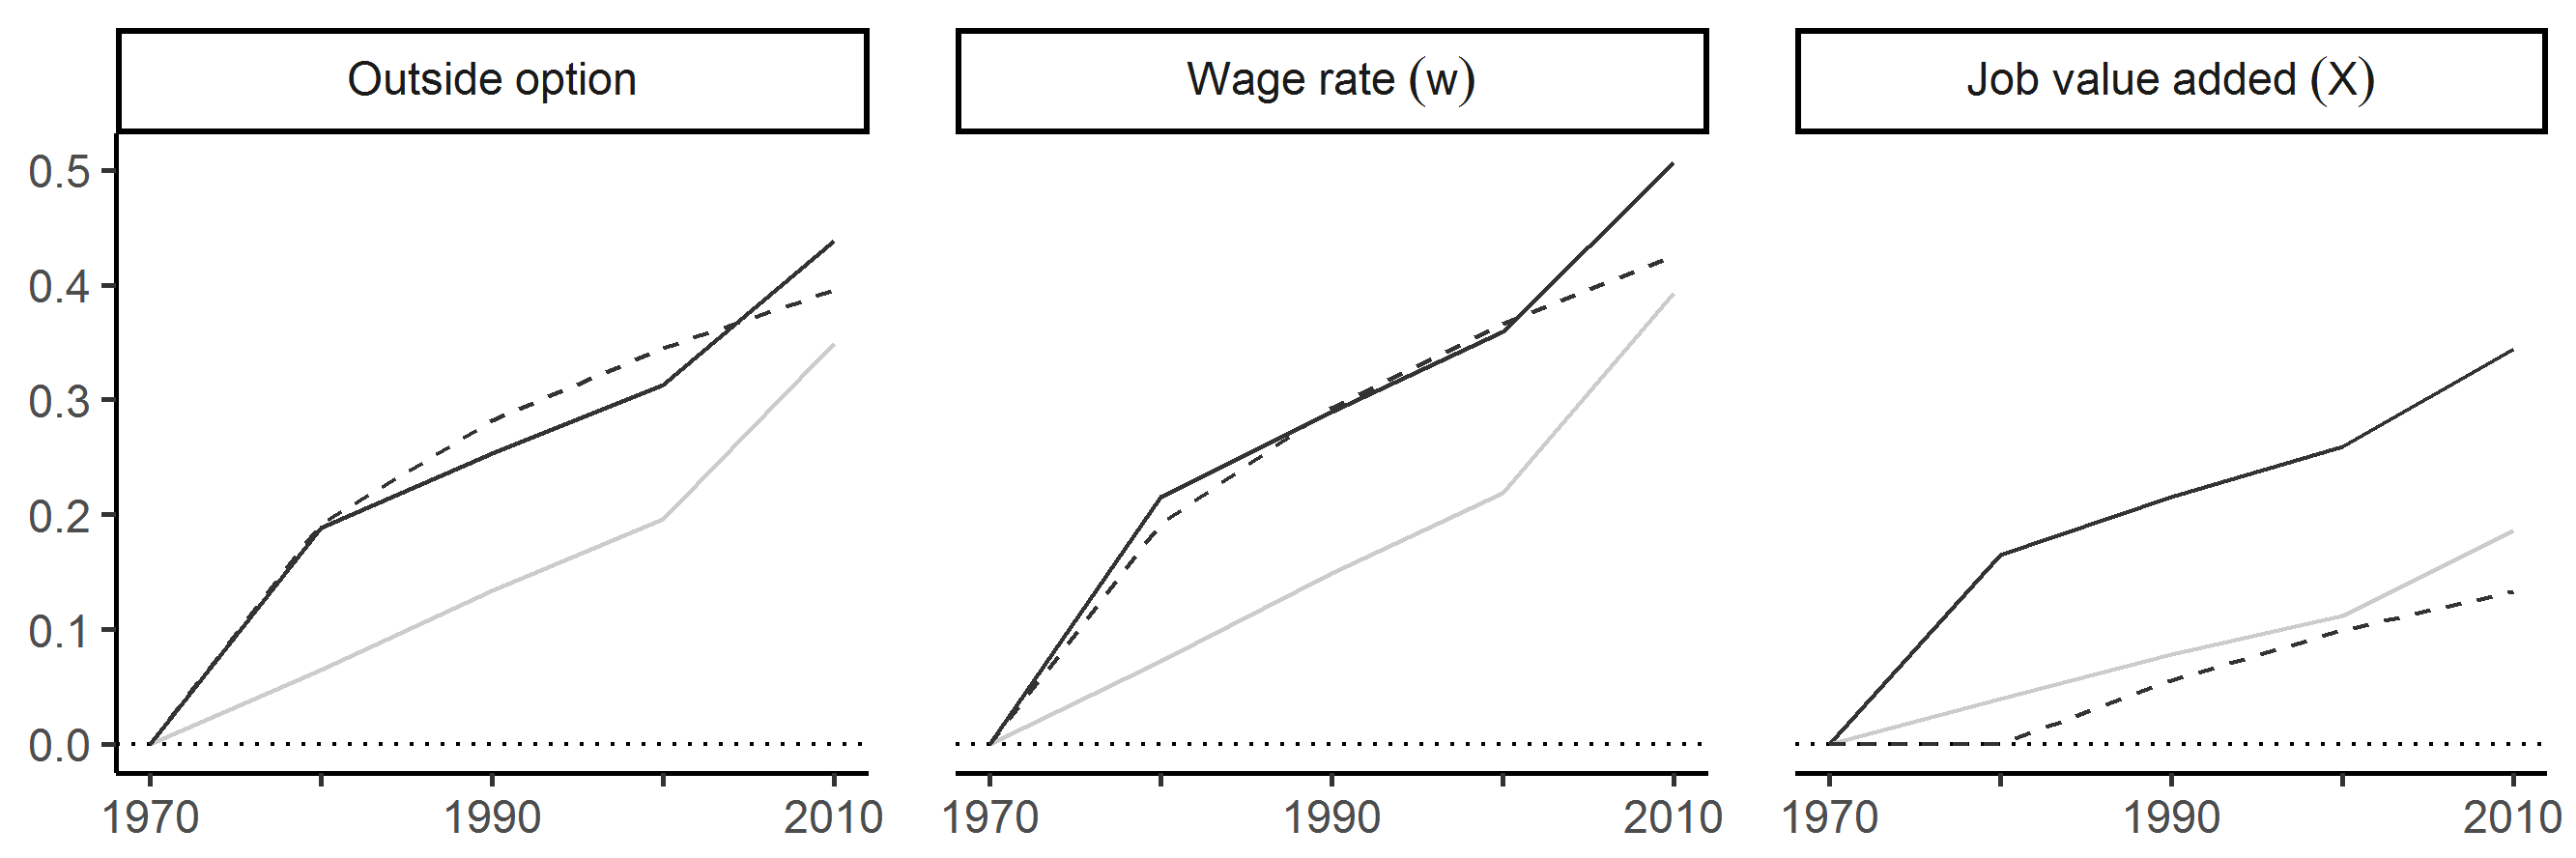
\includegraphics[width=1\linewidth]{../result/deviation/dev_bargain7010.png}
	\caption{Deviation from the 1970 steady-state of wage bargaining variables}
	\label{fig:dev_bargain7010}
	\vspace{.5ex}
	\hrule
	\vspace{-4ex}
	\justify\singlespacing\footnotesize \textit{Notes:} The outside option corresponds to $b/(1-\tau)$. The reader is referred to the footnote of the figure \ref{fig:dev_public7010} for the legend of the curves.
\end{figure}
Pro-youth public policies motivated by a higher youth political weight leads to an increase of the unemployment benefits and a decline of the disposable income rate $(1-\tau_t)$. These two variables determine the outside option $b_t/(1-\tau_t)$ within the wage bargaining. The decrease of the denominator exceeds the increase of the numerator. Thus, the net effect on the outside option is positive and allows workers to bargain a greater wage $w_t$. The gain in net wage $(1-\tau_t)w_t$ exceeds the one in unemployment benefits per capita $b_t$. Hence, employment is even more worth as unemployment in terms of utility (i.e. $dX_t > 0$).

% Production
Due to the ability of workers to bargain a greater wage, the representative firm shifts away from labor. Figure \ref{fig:dev_prod7010} displays the deviation from the 1970 steady-state of production function variables in percentage.
\begin{figure}[tb]
	\centering
	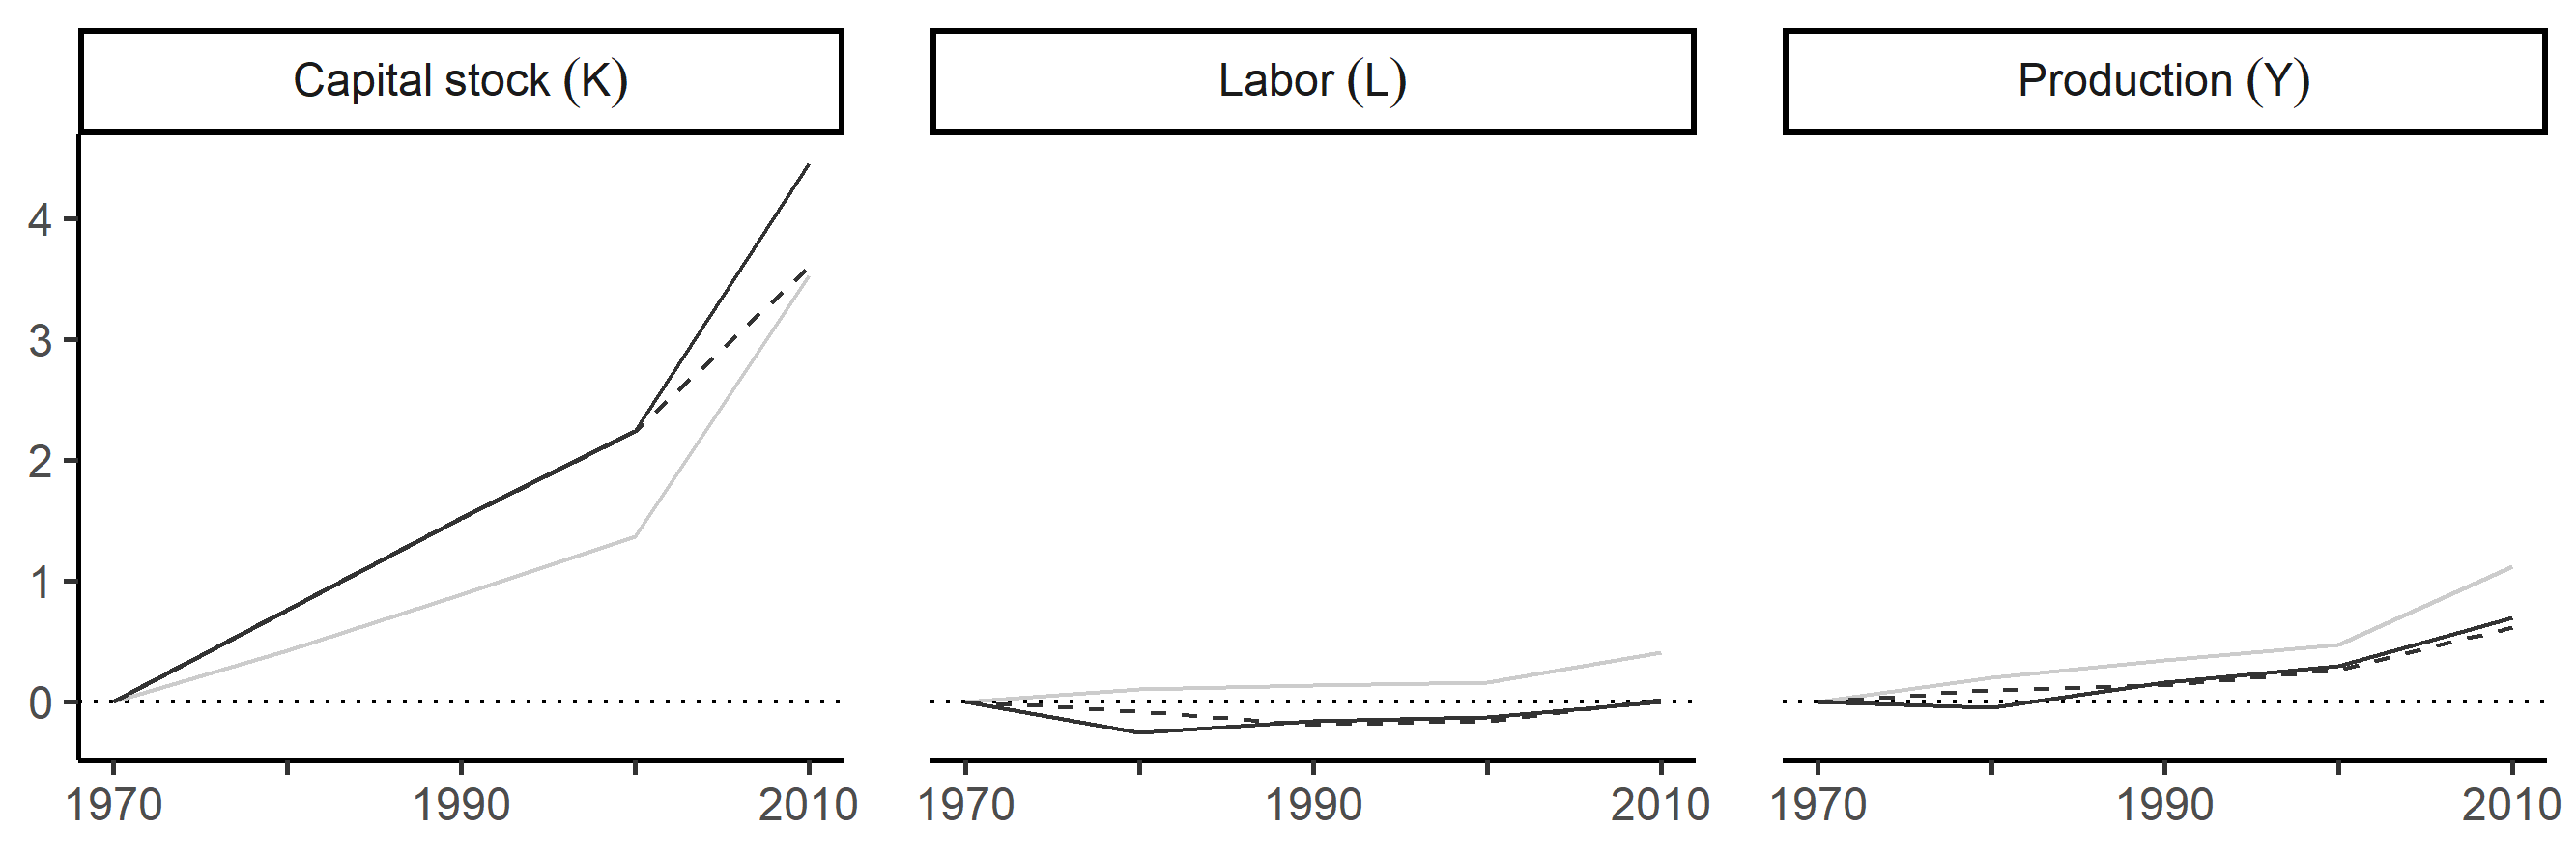
\includegraphics[width=1\linewidth]{../result/deviation/dev_prod7010.png}
	\caption{Deviation from the 1970 steady-state of production function variables}
	\label{fig:dev_prod7010}
	\vspace{.5ex}
	\hrule
	\vspace{-4ex}
	\justify\singlespacing\footnotesize \textit{Notes:} The reader is referred to the footnote of the figure \ref{fig:dev_public7010} for the legend of the curves.
\end{figure}
This behavior is permitted by two features of the model. First, the right-to-manage specification of the wage bargaining enables the firm to hire and fire as much as wanted. Second, the capital-labor elasticity of substitution $\sigma$ is greater than unity for both countries. Thus, both input factors are gross substitute. The firm is able to substitute labor with capital for a given output level. This behavior leads to a decline of the number of worker $L_t$ because the labor cost (i.e. the wage) has increased. Notice that the substitution effect is more vigorous in France because of the relatively higher elasticity of substitution $\sigma$. French firms are able to substitute relatively more labor with capital and also have a faster growth in capital stock $K_t$. Thus, the number of workers becomes lower than its 1970's level in France. While the United-States manage to slightly increase its labor factor. As a consequence, the US production $Y_t$ grows faster.

% Unemployment
The slowdown in employment has consequences on the labor market. Figure \ref{fig:dev_unemp7010} displays the deviation from the 1970 steady-state of unemployment's component variables in percentage.
\begin{figure}[tb]
	\centering
	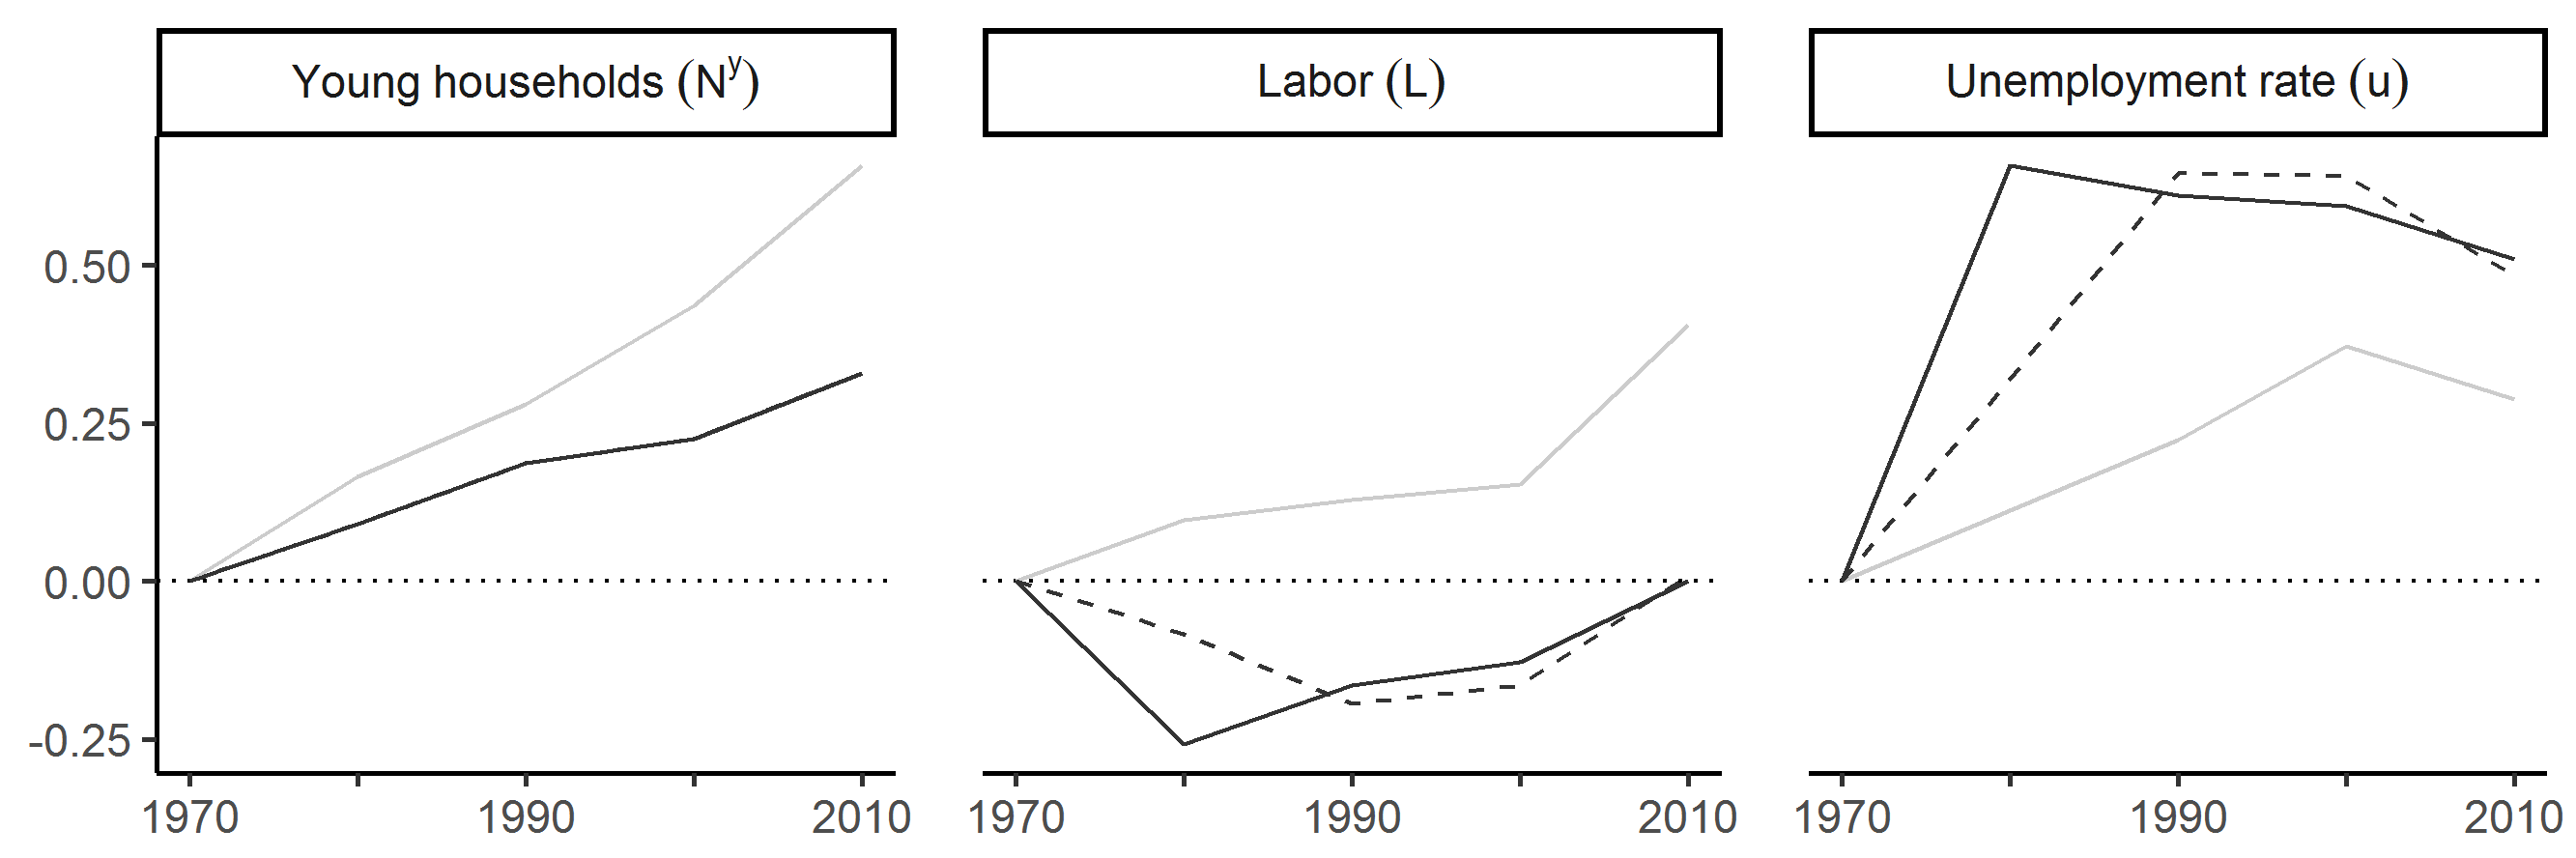
\includegraphics[width=1\linewidth]{../result/deviation/dev_unemp7010.png}
	\caption{Deviation from the 1970 steady-state of unemployment's component variables}
	\label{fig:dev_unemp7010}
	\vspace{.5ex}
	\hrule
	\vspace{-4ex}
	\justify\singlespacing\footnotesize \textit{Notes:} The reader is referred to the footnote of the figure \ref{fig:dev_public7010} for the legend of the curves.
\end{figure}
This slowdown in employment directly raises unemployment in France by reducing the number of workers. Furthermore, the effect is all the more tremendous because the labor force $N_t^y$ grows due to the baby-boomers' arrival. The United-States also know a growing population but the impact on unemployment is much weaker due to the increasing number of workers, as discussed above.

% Labor share components
The dynamics of the production function affects the determinants of the labor share. Figure \ref{fig:dev_laborshare7010} displays the deviation from the 1970 steady-state of labor share's component variables in percentage.
\begin{figure}[tb]
	\centering
	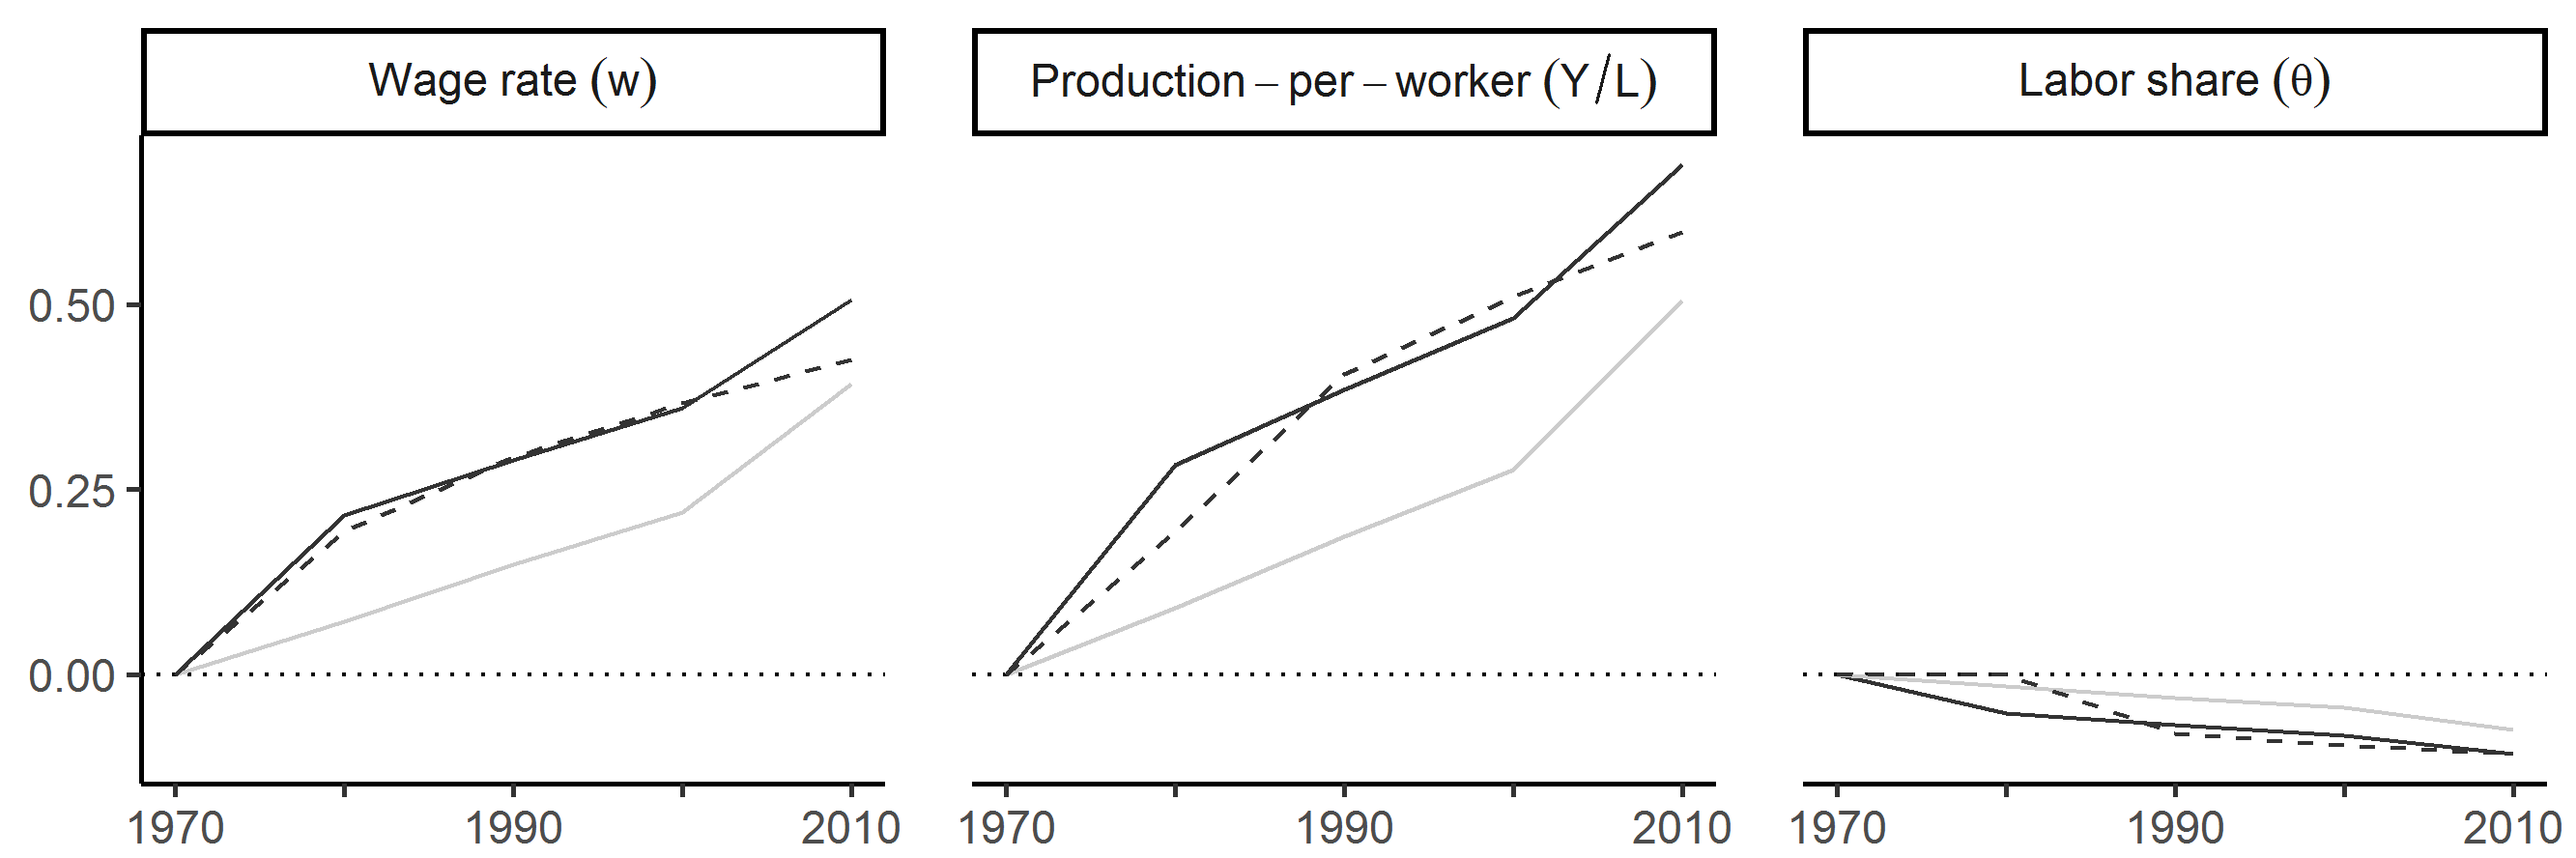
\includegraphics[width=1\linewidth]{../result/deviation/dev_laborshare7010.png}
	\caption{Deviation from the 1970 steady-state of labor share's component variables}
	\label{fig:dev_laborshare7010}
	\vspace{.5ex}
	\hrule
	\vspace{-4ex}
	\justify\singlespacing\footnotesize \textit{Notes:} The reader is referred to the footnote of the figure \ref{fig:dev_public7010} for the legend of the curves.
\end{figure}
Due to the fact that both input factors are gross substitute, the output-per-worker $Y_t/L_t$ increases when the capital-per-worker $k_t$ does so. This increase exceeds the one of the wage. As a result, the labor share declines.

Let summarize the mechanisms over this period. The youth fosters a pro-labor public policy due to a relatively high political weight. This institutional design raises the outside option of the workers. It gives more bargaining power to the union who is able to bargain greater wages. The cost of labor becoming too high, the firms decide to shift away from labor. The fact that both input factors are gross-substitute allows firms to substitute labor with capital. The shift-away from labor engenders an increase of the output-per-worker which thwarts and exceeds the wage gain. Thus, the labor share declines. Moreover, unemployment rises due to a growing labor force.

\subsection{Model predictions over the period 2010-2080}

\subsubsection{The labor share resurgence}

%% Description of the graph
Figure \ref{fig:baseline1080} displays the model predicted labor share over the period 1970-2080.
\begin{figure}[tb]
	\centering
	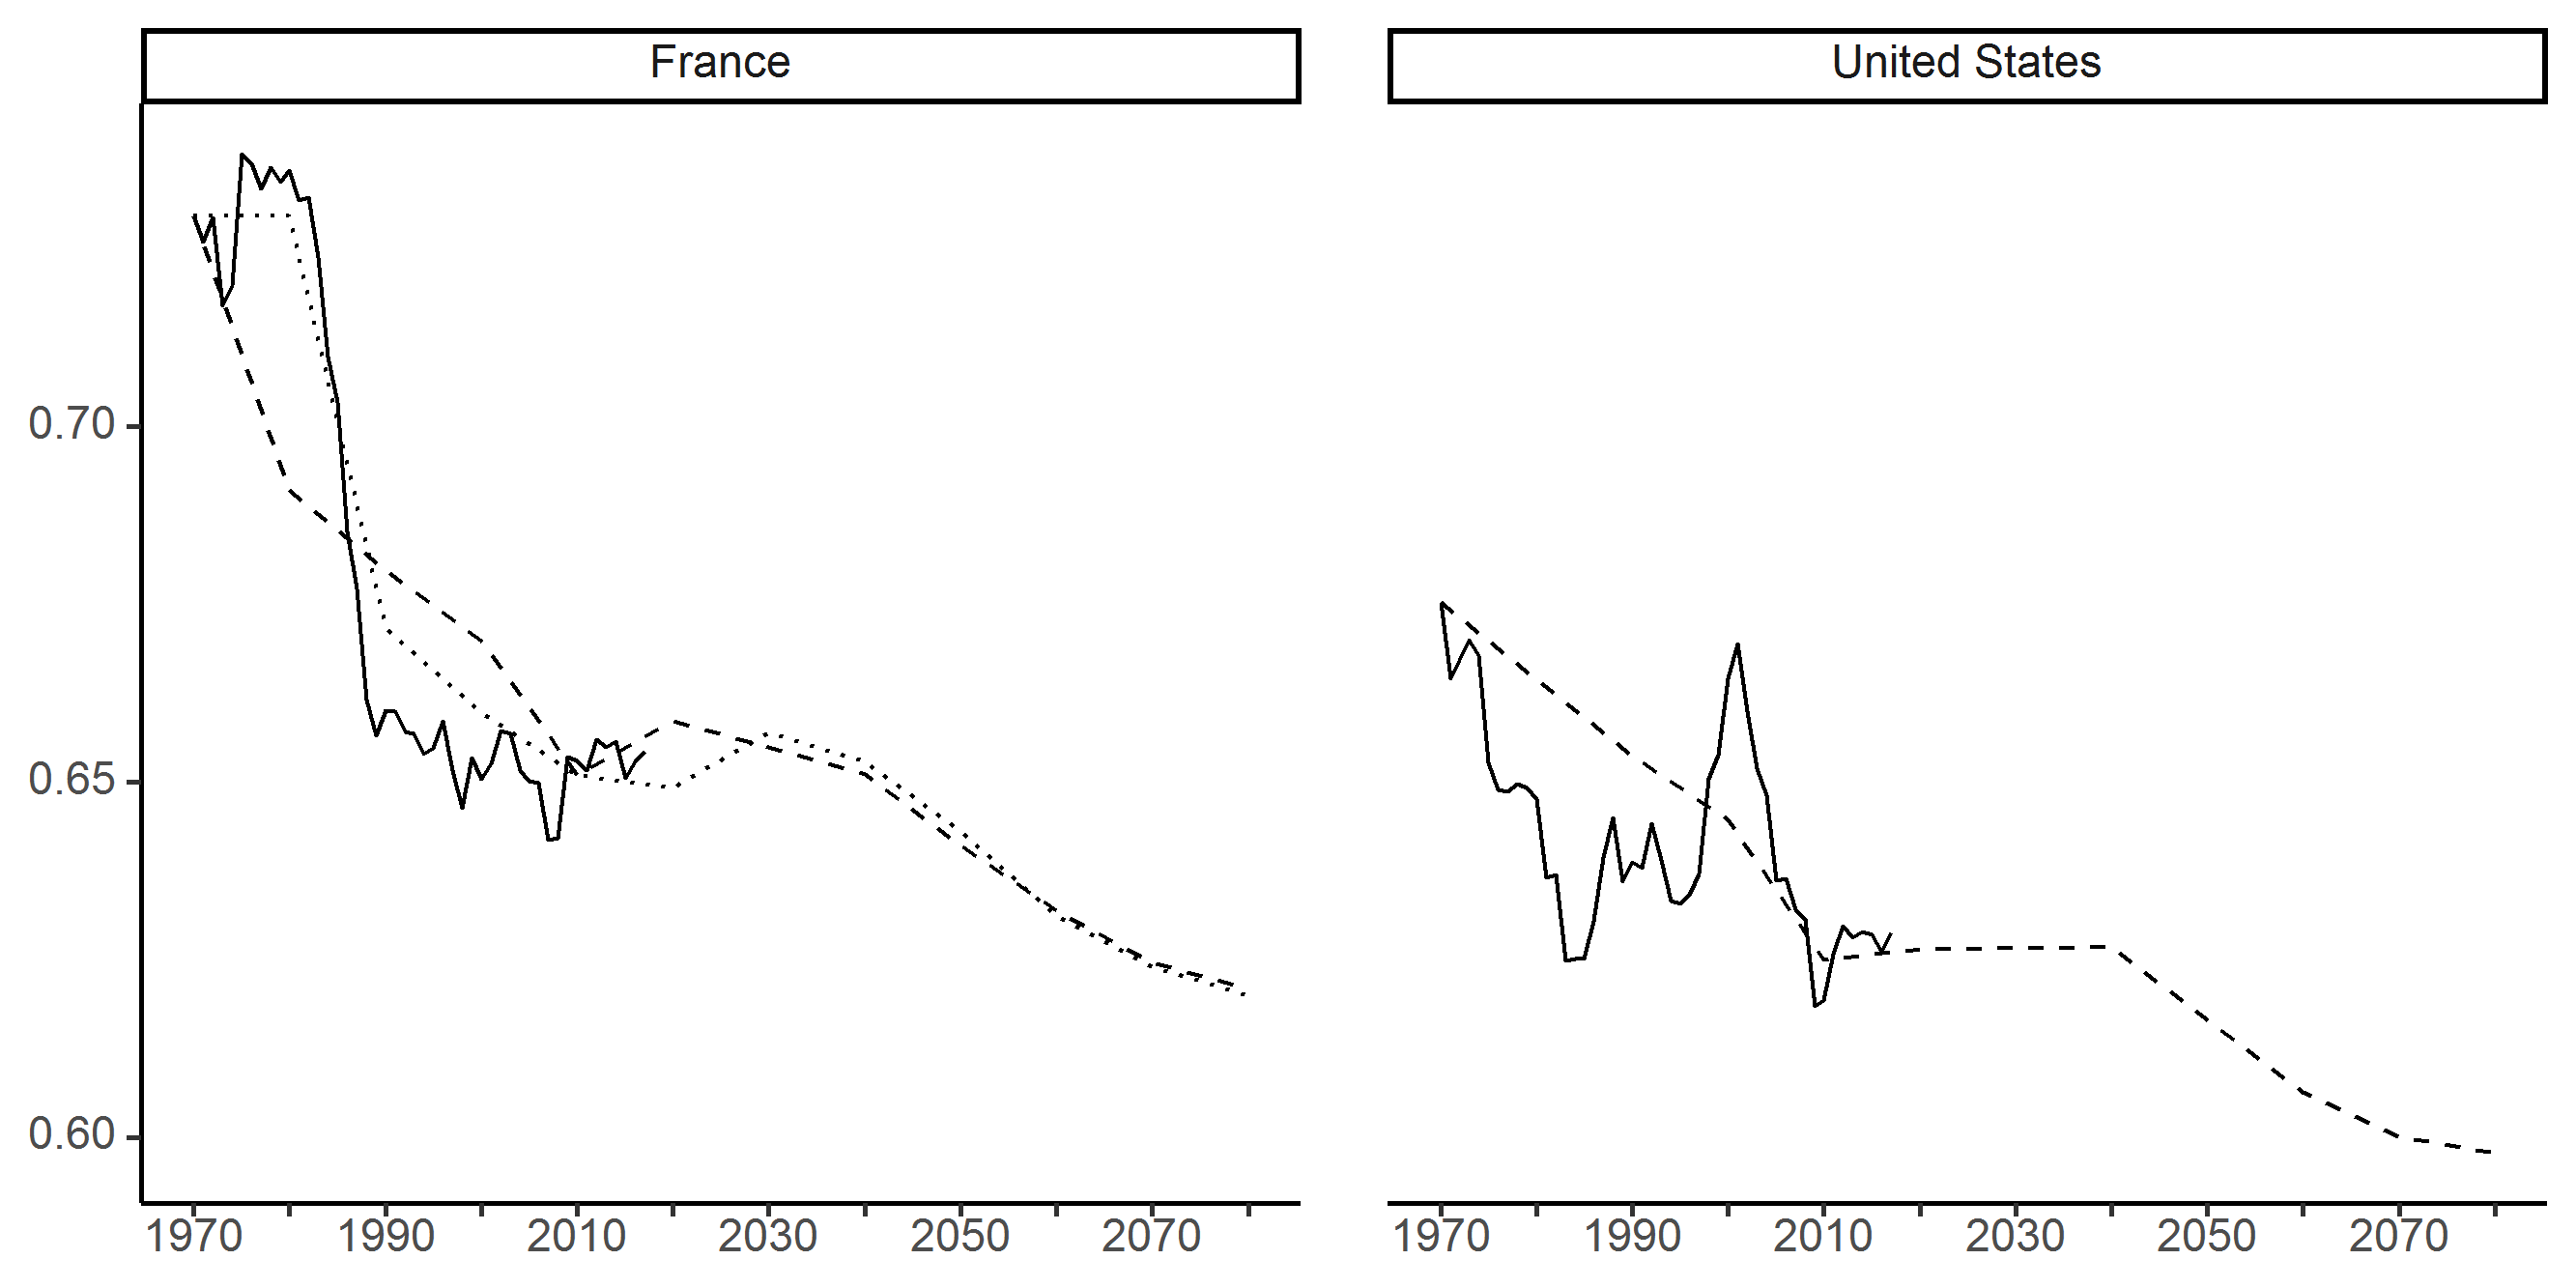
\includegraphics[width=1\linewidth]{../result/baseline7080.png}
	\caption{Model prediction of the labor share}
	\label{fig:baseline1080}
	\vspace{.5ex}
	\hrule
	\vspace{-4ex}
	\justify\singlespacing\footnotesize \textit{Notes:} The reader is referred to the footnote of the figure \ref{fig:baseline7010} for the legend of the curves.
\end{figure}
The model predicts that the labor share should continue to decline during the next decades in both countries. However, France should face a slight rise in 2020 up to 65.9 \% before to shrink again.\footnote{Under the model specification with a break in the regime of $\sigma$ for France (i.e. the dotted curve), the peak occurs in 2030 with a labor share up to 66.1 \%.} While the US labor share should remain stable around 62.6 \% between 2010 and 2040 and then follow the same pattern.

\subsubsection{Mechanisms of the resurgence}

The demographic context over the period 2010-2080, as presented in figure \ref{fig:demo}, is roughly the same for France and the United-States. The population growth $n_t$ faces a sharp decline between 2010 and 2050 before to stabilize thereafter. Meanwhile, the survival rate $p_t$ grows around 4\% per decades on average. Thus, the old-age-dependency ratio skyrockets until 2050. Once the population growth becomes stable, the ratio still grows but at a lower rate. This important aging of the population is mainly due to the baby-boomers' retirement. As a result of this demographic context, the youth political weight $\eta_t$ never gets back to its 2010's level and will strongly decline until 2050 for both countries.

% The story is the opposite of the period 1970-2010.

% Public Policy
Figure \ref{fig:dev_public1080} displays the deviation from the 1970 steady-state of public policy variables in percentage.
\begin{figure}[tb]
	\centering
	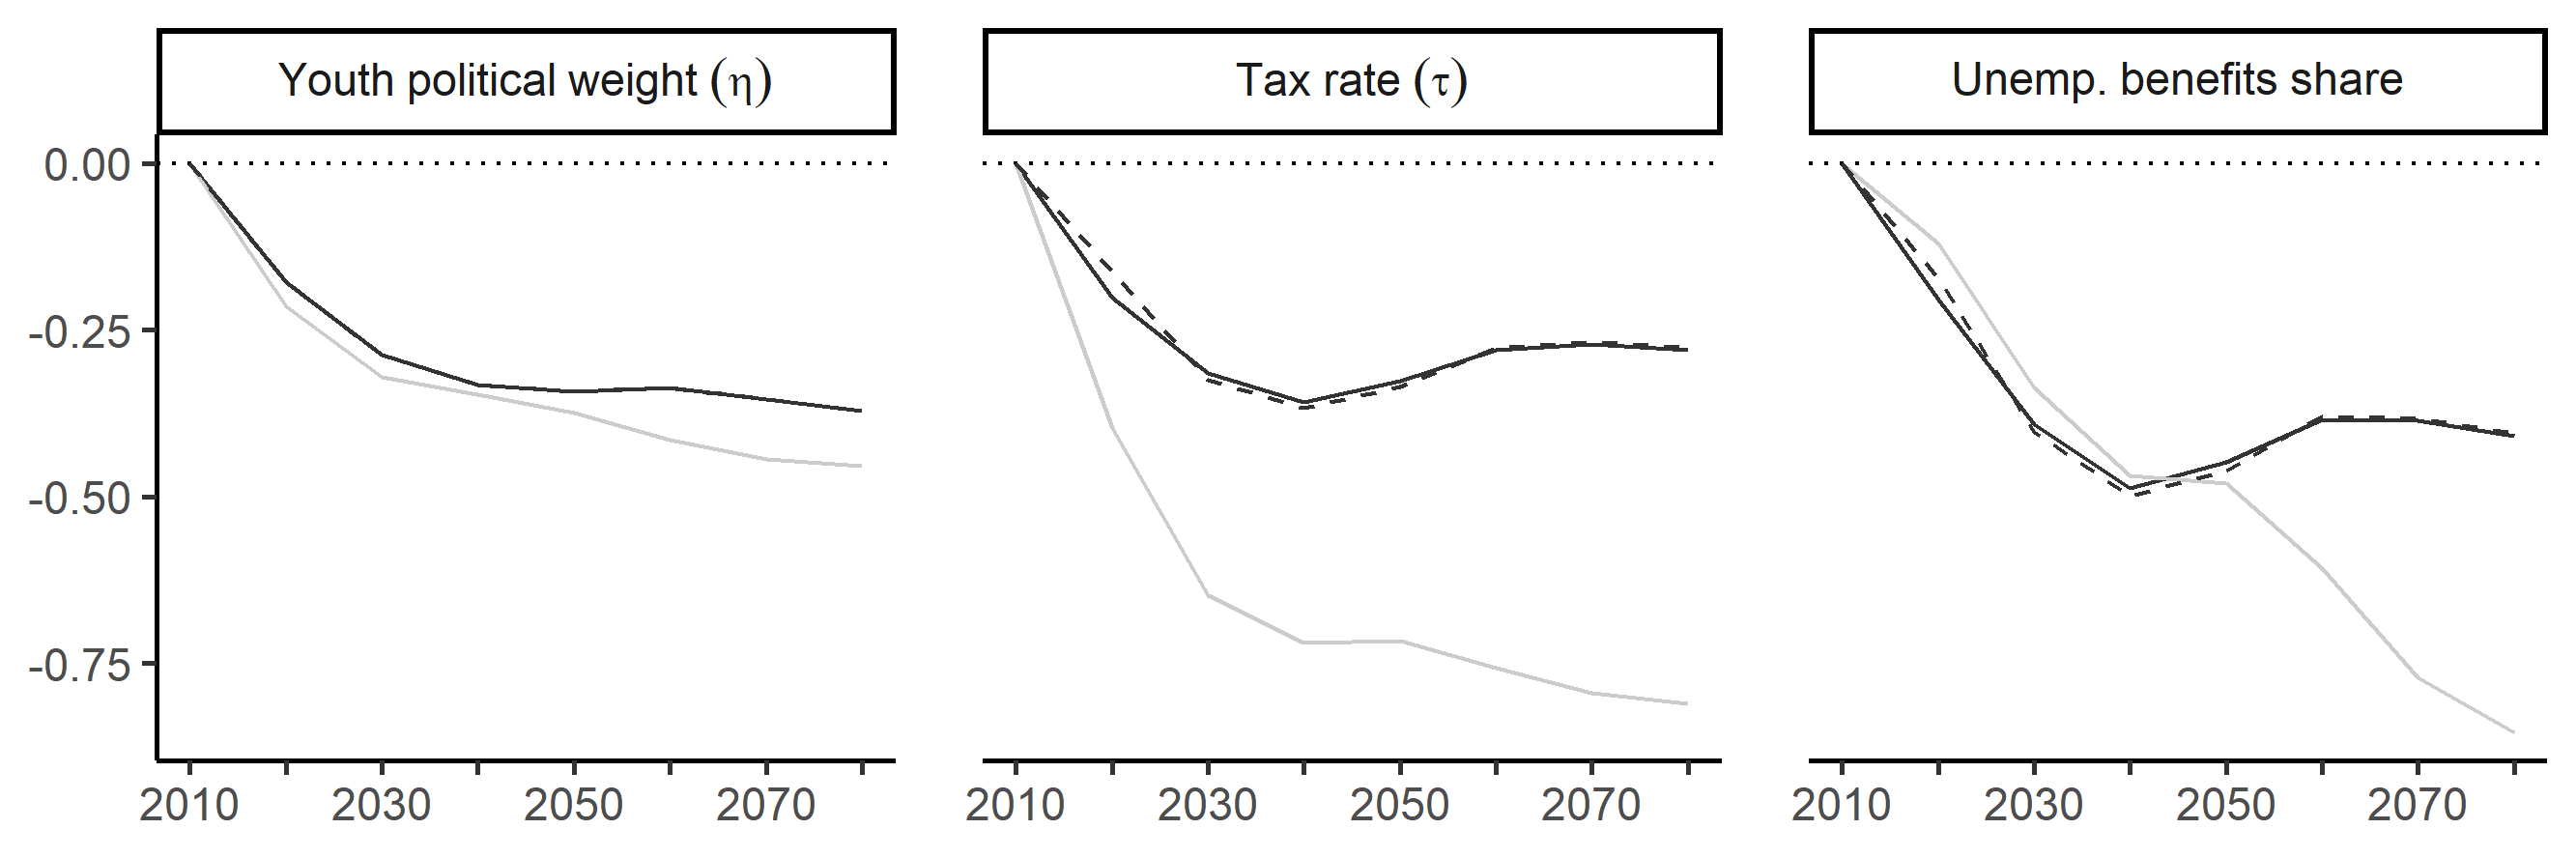
\includegraphics[width=1\linewidth]{../result/deviation/dev_public1080.png}
	\caption{Deviation from the 2010 steady-state of public policy variables}
	\label{fig:dev_public1080}
	\vspace{.5ex}
	\hrule
	\vspace{-4ex}
	\justify\singlespacing\footnotesize \textit{Notes:} The unemp. benefits share corresponds to the share of the unemployment benefits in the government spending, i.e. $buN^y/(\tau Y)$. The reader is referred to the footnote of the figure \ref{fig:dev_public7010} for the legend of the curves.
\end{figure}
The young political weight $\eta_t$ sharply declines due to the aging of the population. Thus, opportunist political candidates favor old households who desire less redistribution (i.e. $\partial\tau_t / \partial \eta_t > 0)$. Pro-elderly public policies are implemented. In terms of the model, it is translated by an increase of the health spending share in government revenue at the cost of the unemployment benefits one $b~share$.

% Wage bargaining
These policy changes interact with the wage bargaining because they affect the outside option of young households. Figure \ref{fig:dev_bargain1080} displays the deviation from the 2010 steady-state of wage bargaining variables in percentage.
\begin{figure}[!b]
	\centering
	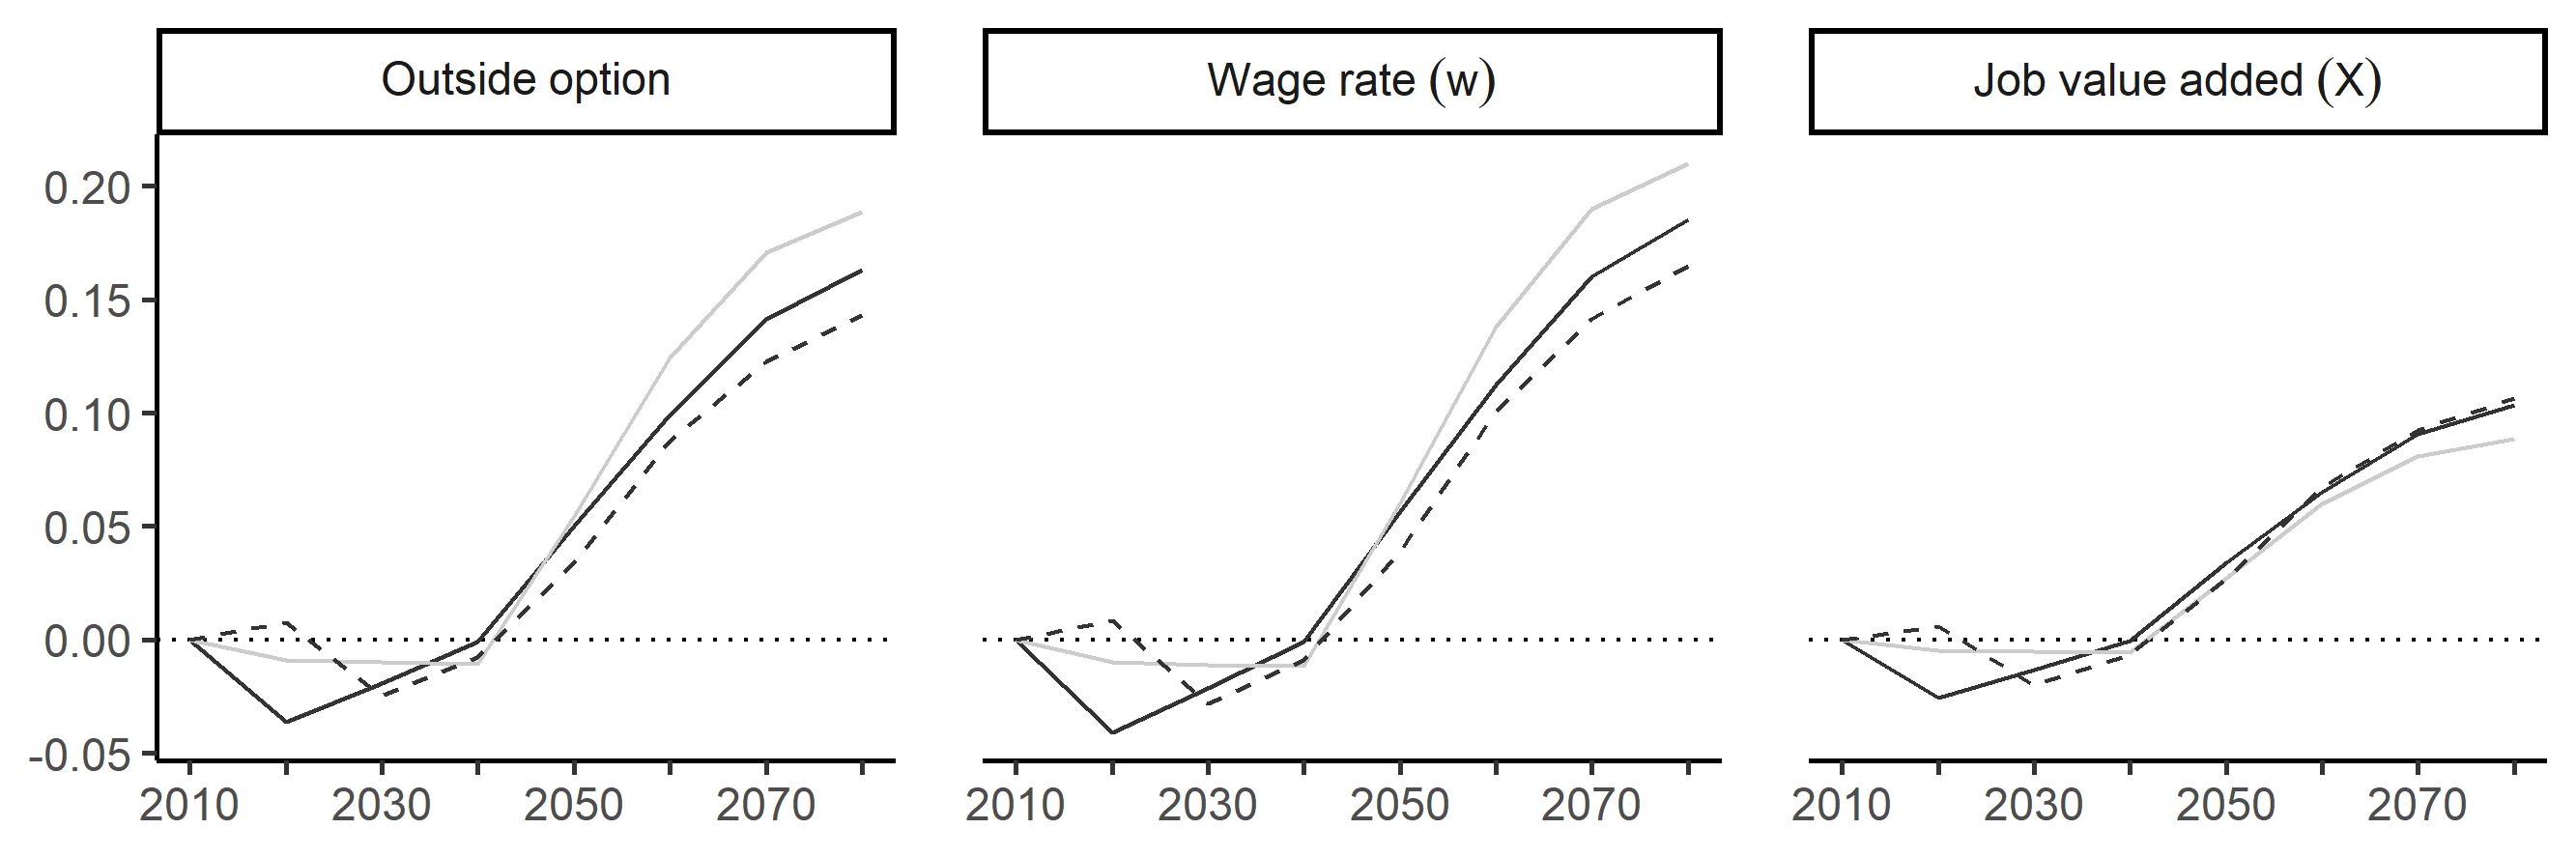
\includegraphics[width=1\linewidth]{../result/deviation/dev_bargain1080.png}
	\caption{Deviation from the 2010 steady-state of wage bargaining variables}
	\label{fig:dev_bargain1080}
	\vspace{.5ex}
	\hrule
	\vspace{-4ex}
	\justify\singlespacing\footnotesize \textit{Notes:} The outside option corresponds to $b/(1-\tau)$. The reader is referred to the footnote of the figure \ref{fig:dev_public7010} for the legend of the curves.
\end{figure}
Pro-elderly public policies leads to slightly weaken the outside option $b_t/(1-\tau_t)$ within the wage bargaining for both countries between 2010 and 2050. Workers are no longer in position to bargain greater wages and have to concede a wage cut. Hence, having a job between 2010 and 2050 is less worth in terms of utility as it was worth in 2010. But the drawback is not that tough because the declining wage goes along with a decline of the tax rate. In both countries, the outside option rises over the period 2050-2080 and so does the bargained wage. This increase is mainly due to the disappearance of baby-boomers. Thus, the age-related conflict within the public policy becomes relatively more in favor of the youth again.

% Production
Figure \ref{fig:dev_prod1080} displays the deviation from the 2010 steady-state of production function variables in percentage.
\begin{figure}[tb]
	\centering
	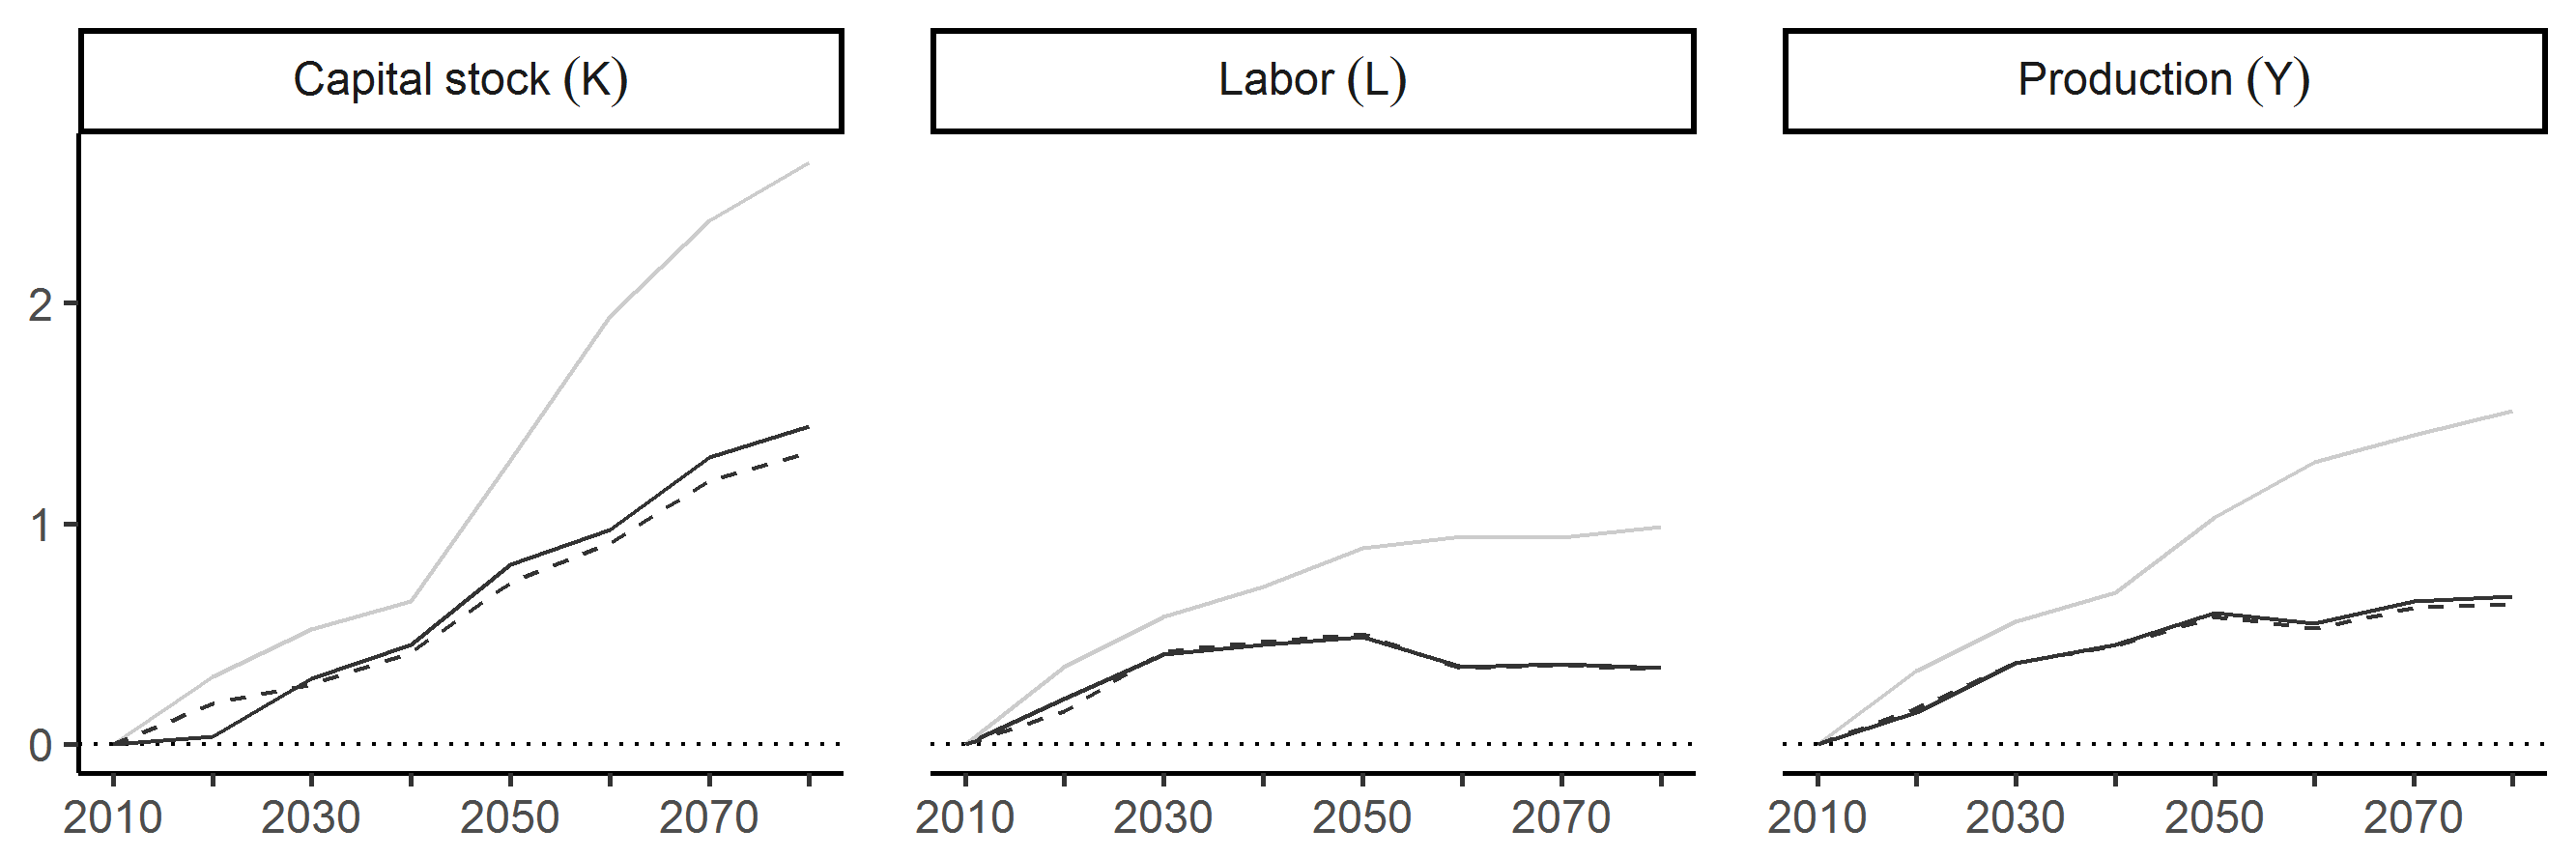
\includegraphics[width=1\linewidth]{../result/deviation/dev_prod1080.png}
	\caption{Deviation from the 1970 steady-state of production function variables}
	\label{fig:dev_prod1080}
	\vspace{.5ex}
	\hrule
	\vspace{-4ex}
	\justify\singlespacing\footnotesize \textit{Notes:} The reader is referred to the footnote of the figure \ref{fig:dev_public7010} for the legend of the curves.
\end{figure}
As the wage decreases between 2010 and 2050, the representative firm has incentive to hire. Thus, the labor $L_t$ does increase over this period. Meanwhile, the capital stock $K_t$ has increased due to savings $S_t$ of the previous periods. Thus, both input factors increase and so does the production $Y_t$. After 2050, France and the United-States diverge in their trajectories. On one hand, the US capital stock rises due to high savings of the previous periods.\footnote{This increase in savings owes to the baby-boomers cohort when they were young. Their massive entry on the labor market, rising expected life expectancy and higher wages have fostered savings and therefore the capital available in the economy once old.} This rise is strong enough to foster the representative firm to hire workers. Thus, the substitution mechanism does not undertake. On the other hand, the increase of the French capital stock does not follow the same exploding pattern. The french representative firm, as during the end of the twentieth century, shifts away from labor and decreases the number of workers. This divergence also appears on the labor market.

% Unemployment
Figure \ref{fig:dev_unemp1080} displays the deviation from the 2010 steady-state of unemployment's component variables in percentage.
\begin{figure}[tb]
	\centering
	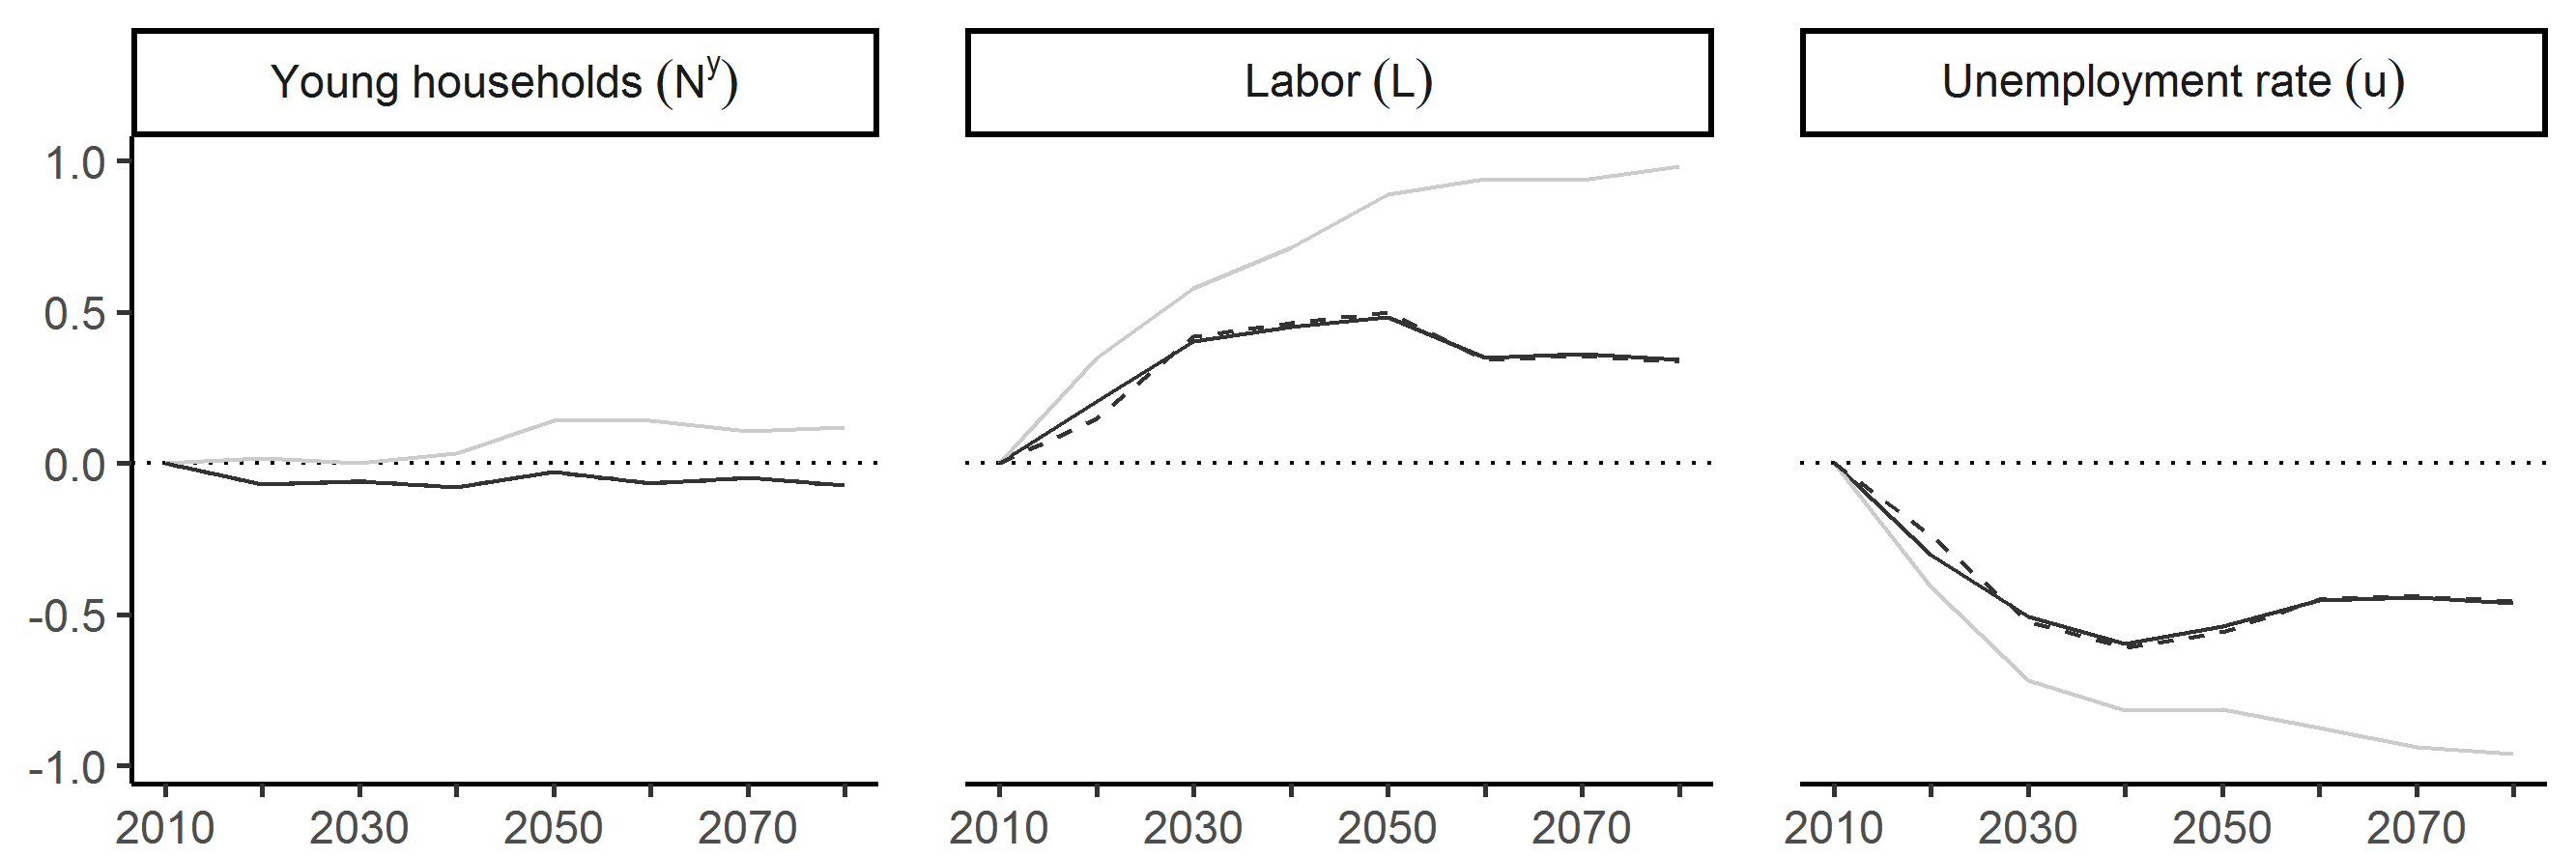
\includegraphics[width=1\linewidth]{../result/deviation/dev_unemp1080.png}
	\caption{Deviation from the 2010 steady-state of unemployment's component variables}
	\label{fig:dev_unemp1080}
	\vspace{.5ex}
	\hrule
	\vspace{-4ex}
	\justify\singlespacing\footnotesize \textit{Notes:} The reader is referred to the footnote of the figure \ref{fig:dev_public7010} for the legend of the curves.
\end{figure}
The labor force $N^y_t$ is roughly constant over the whole period and France is even below its 2010's level. Thus, the number of workers variations $L_t$ mainly drives the unemployment ones. The unemployment rate decreases in the United-States over the whole period. It falls down to 1.69\% by 2080 against 44.6\% in 2010. Here again, the sharp increase of the capital stock fosters employment until almost full-employment. The french unemployment rate decreases until 2050 before to slightly rise a bit and stabilize itself around 26.9\% in 2080.

% Labor share
Figure \ref{fig:dev_laborshare1080} displays the deviation from the 2010 steady-state of labor share's component variables in percentage.
\begin{figure}[tb]
	\centering
	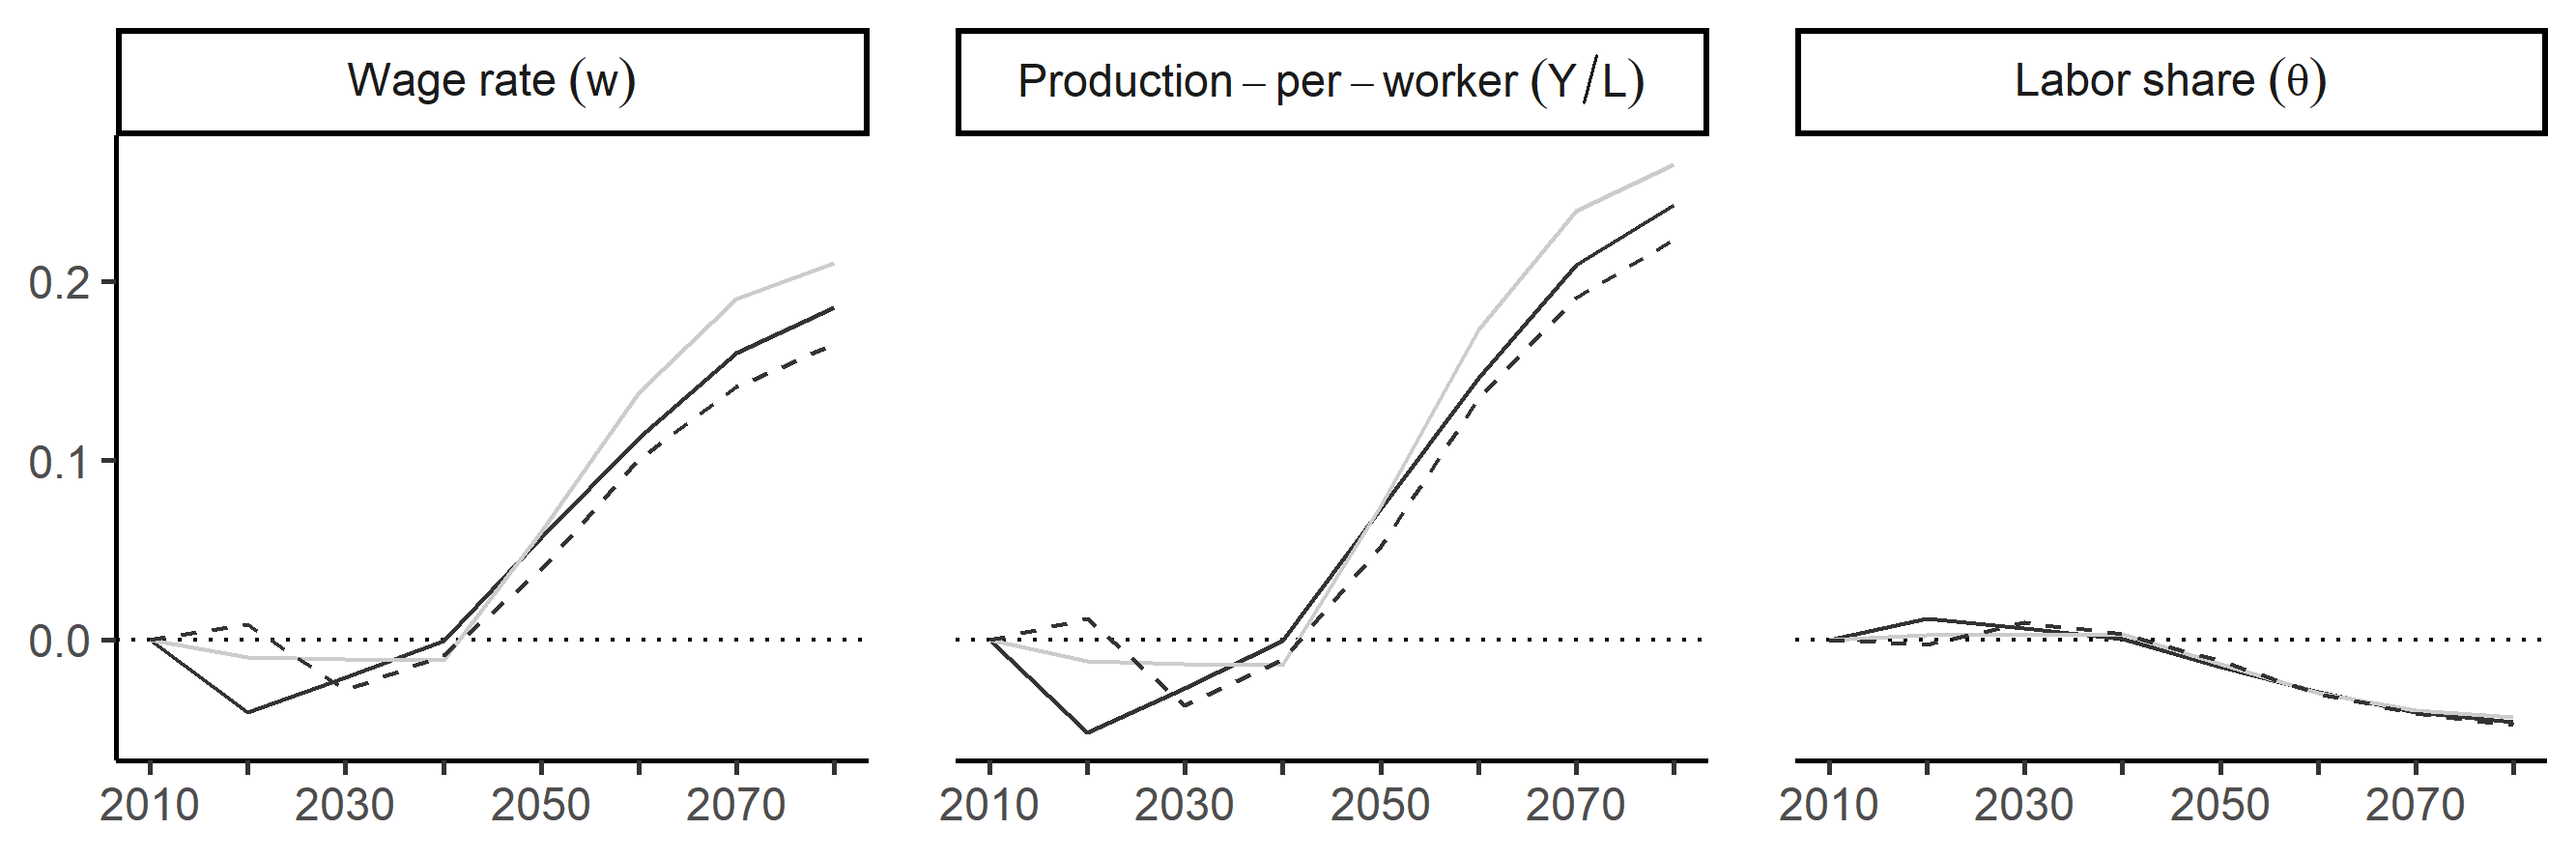
\includegraphics[width=1\linewidth]{../result/deviation/dev_laborshare1080.png}
	\caption{Deviation from the 2010 steady-state of labor share's component variables}
	\label{fig:dev_laborshare1080}
	\vspace{.5ex}
	\hrule
	\vspace{-4ex}
	\justify\singlespacing\footnotesize \textit{Notes:} The reader is referred to the footnote of the figure \ref{fig:dev_public7010} for the legend of the curves.
\end{figure}
French and US workers experience a minor reduction of their wage $w_t$ between 2010 and 2050 and so does the output-per-worker $Y_t/L_t$. The latter being greater than the former, the French labor share slightly increases. The US labor share remains constant because both variations compensate. After 2050, both labor shares decline to reach 62\% and 59.8\%, respectively for France and the United-States. While their respective levels in 2010 were 65.1\% and 62.5\%.

\subsection{Counterfactual and aging effect decomposition} \label{subsec:counterfactual}

So far, I have highlighted the different mechanisms through which the age structure of the population affects economic variables and therefore the labor share. For the remaining part of the paper, I consider that the previous model prediction is the benchmark prediction. For the french case, I envisage the model specification with a break in the regime of $\sigma$. To summarize, demographic changes are due to two determinant variables in the model : the population growth $n_t$ and the survival rate $p_t$. These variations may affect the labor share through two channels : the direct cohort effect $n_t$, $p_t$, $p_{t+1}$ and the indirect cohort effect $\eta_t(n_t, p_t, p_{t+1})$.

I make counterfactual predictions in order to quantity the respective role of each determinants and channels. The principle is to neutralize either a determinant of the demographic change or a channel through which the labor share is affected. The intuition behind the counterfactual is to observe what would have happened in terms of model predictions if this effect/channel was neutralized. By comparing a counterfactual simulation to the benchmark one, I can quantify its extent. I proceed in two steps. First, I examine the impact of the different determinants of demographic changes (i.e. $n_t$ versus $p_t$). Second, I investigate through which channels it occurs (i.e. direct versus indirect).

\subsubsection{Survival rate and population growth effects}

To neutralize the impact of the survival rate $p_t$, I assume that it remains at its 1970's level. Thus, $p_t = p_{1970}$ and $p_{t+1} = p_{2010}$. Old household population size is recalculated such that ${N^o_t}^\prime = N_t^o\times\frac{p_{1970}}{p_t}$. Moreover, $\eta_t = \frac{n_t}{p_{1970}}\frac{1+\alpha p_{2010}}{\omega}$.
%\footnote{For the first sequence of the model: 1970, 2010, 2050, \dots . The expected survival rate $p_{t+1}$ in 1970 is not equal to $p_{1970}$ but to $p_{2010}$. This exception is done in order to match the benchmark simulation in 1970 and thus share the same fixed point. Otherwise, $\eta^{\text{bench.}}_{1970} \neq \eta^{p}_{1970} \Rightarrow k^{\text{bench.}}_{1970} \neq k^{p}_{1970} \Rightarrow \theta^{\text{bench.}}_{1970} \neq \theta^{p}_{1970}$, where $^\text{bench.}$ stands for the benchmark simulation and $^p$ for the constant survival rate simulation.}
The other demographic variables (i.e. $n_t$ and $N^y_t$) follow the time series of the benchmark simulation. The initial capital stocks of the four sequences are also recalculated such that $K_0^\prime = \frac{1+\alpha p_t}{p_t}\frac{p_{1970}}{1+\alpha p_{1970}} K_0$.\footnote{Setting constant the survival rate implies changes in the saving rate through the expected survival rate $p_{t+1}$. $K_0 \equiv S_{-1} = \frac{\alpha p_0}{1+\alpha p_0}\left[(1-\tau_{-1})w_{-1}(1-u_{-1})+b_{-1}u_{-1}\right]N_{-1}^y$. In order to assess the true impact of the survival rate, it is also necessary to consider saving rate changes in the counterfactual simulation. Thus, the initial capital stocks for the first periods of the four sequences becomes $K_0^\prime = \frac{1+\alpha p_t}{p_t}\frac{p_{1970}}{1+\alpha p_{1970}} K_0$. Notice that a change in the survival rate $p_0$ should also affect the aggregated disposable income of young households in $t=-1$, i.e. $(1-\tau_{-1})w_{-1}(1-u_{-1})+b_{-1}u_{-1}$. However, I do not consider this source of change. Notice also that the term $N_{-1}^y$ does not change because $N_{-1}^y = \frac{N_0^o}{p_0} = \frac{{N_0^o}^\prime}{p_{1970}}$.} The methodology is analogous to neutralize the impact of the population growth but with $n_t = n_{1970}$, ${N_t^y}^\prime = N_t^y\times\frac{n_{1970}}{n_t}$ and $\eta_t = \frac{n_{1970}}{p_t}\frac{1+\alpha p_{t+1}}{\omega}$.\footnote{In this specification, the initial capital stocks are not changed because $n_0$ does not affect $S_{-1}$.} Finally, a last counterfactual is made to neutralize both effects. So, $p_t = p_{1970}$, $p_{t+1} = p_{2010}$, $n_t = n_{1970}$ and $\eta_t = \eta_{1970}$. As before, population sizes and initial capital stock values are recalculated.
%\footnote{The same exception, as explained in the previous footnote, is done to ensure that the labor share in matched in 1970.}
Here, the old-age-dependency ratio remains constant. Table \ref{tab:demo1970} summarizes demographic variables in 1970.
\begin{table}[tb]
	\caption{Demographic variables in 1970}\label{tab:demo1970}
	\centering
	\begin{threeparttable}
		\begin{tabular}{c l D{.}{.}{-3} D{.}{.}{-3}}
			\multicolumn{2}{c}{\textbf{Variable}} & \multicolumn{1}{r}{\textbf{France}} & \multicolumn{1}{r}{\textbf{United-States}}            \\ \hline \hline
			$p_{1970}$           	& Survival rate in 1970         					  & 0.417 & 0.476		\\
			$n_{1970}$          	& Population growth in 1970                           & 1.134 & 1.597		\\
			$p_{2010}$           	& Expected survival rate in 2010         			  & 0.583 & 0.561		\\
			$\frac{p_{1970}}{n_{1970}}$     & Old-age-dependency ratio in 1970         	  & 0.368 & 0.298			\\
			$\eta_{1970}$           & Youth political weight in 1970                      & 3.846 & 3.008		\\ \hline
			\hline
		\end{tabular}
	%	\vspace{-3ex}
	%	\begin{tablenotes}
	%		\vspace{-3ex}
	%		\singlespacing
	%		{\footnotesize
	%			\item \textit{Note :} .
	%		}
	%	\end{tablenotes}
	\end{threeparttable}
\end{table}

Figure \ref{fig:counter_PGSR_1970} displays the model predictions of the labor share with counterfactual specifications.
\begin{figure}[tb]
	\centering
	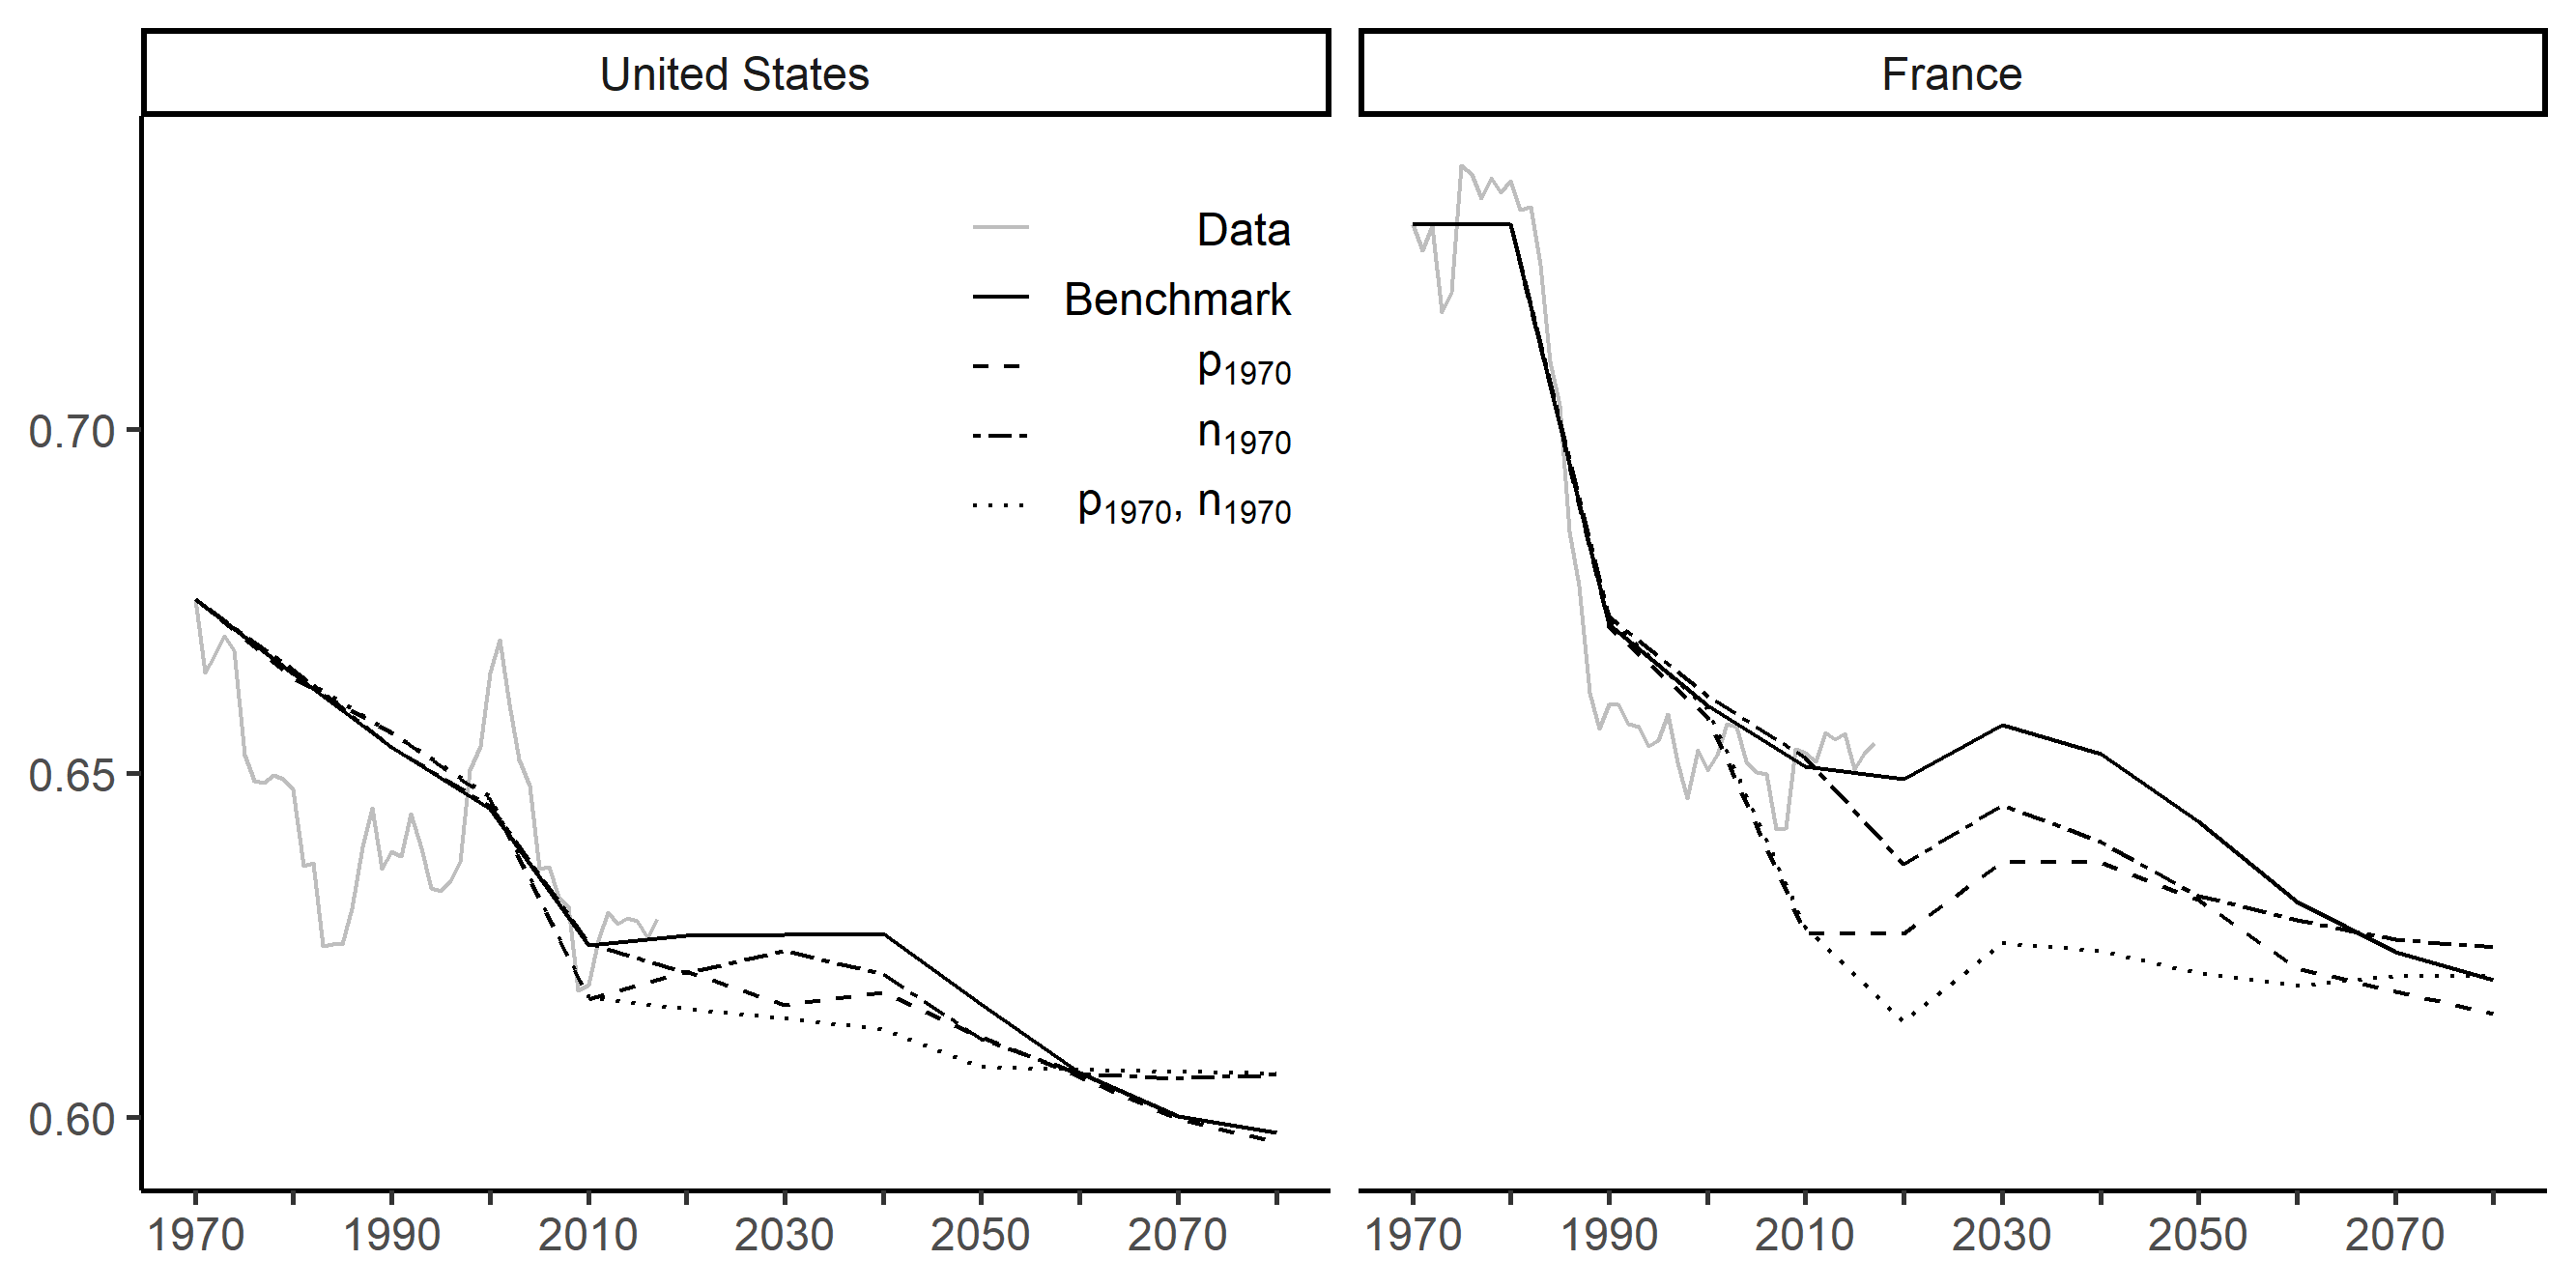
\includegraphics[width=1\linewidth]{../result/decomposition/counter_PGSR.png}
	\caption{Model predictions of the labor share with counterfactual specifications}
	\label{fig:counter_PGSR_1970}
%	\vspace{.5ex}
%	\hrule
%	\vspace{-4ex}
%	\justify\singlespacing\footnotesize 
\end{figure}
To interpret the role played by each demographic variable, I compare each counterfactual time series to the benchmark one. For instance, let start with the impact of the survival rate in France. I look at the dashed curve with respect to the solid one. This curve corresponds to the counterfactual where the survival rate $p_t$ and $p_{t+1}$ remain at their 1970's levels. So, if the survival rate would have not changed, then the labor share would have followed the dashed curve pattern. 
%The blue curve lies below the red one between 1980 and 2020 and above thereafter. Therefore, the survival rate dynamic had a positive impact on the labor share between 1980 and 2020 and a negative one thereafter.
The dashed curve lies below the solid one. Therefore, the survival rate dynamic has a positive impact on the labor share in both countries.
The way to interpret the other counterfactuals is similar.
The dash-dotted curve remains above the solid one until 2050 for France and 2030 for the United States. Until these years, the population growth dynamic has a negative impact on the labor share and a positive one thereafter.
Finally, the dotted curve which corresponds to the counterfactual where both effects are neutralized is below the benchmark simulation. Since 1970, all demographic dynamics have led to increase the labor share with respect to what it would have been without these dynamics.
However, this representation is tediously legible. Therefore, I compute the distance between the benchmark labor share and each counterfactual labor share. Using the Chasles' relation within an affine space at each point in time, it is possible to isolate the extent of each effect.\footnote{Let $r$ (resp. $b, g, p$) be the labor share from the red (resp. blue, green, purple) curve on figure \ref{fig:counter_PGSR_1970}. For a given year, $2\vec{rp} = \vec{rb} + \vec{bp} + \vec{rg} + \vec{gp} \Leftrightarrow \vec{rp} = \vec{rb} + \vec{rg} + \vec{\text{int.}}$, where $\vec{\text{int.}} \equiv \vec{bp} + \vec{gp} - \vec{rp} = \vec{gp} +\vec{br} = \vec{bp} + \vec{gr}$ is the interaction of both effects defined as the part which is not exclusively explained by both effects independently.} Figure \ref{fig:decomp_PGSR} displays the labors share's gap between the benchmark and the counterfactuals in percentage points.
\begin{figure}[tb]
	\centering
	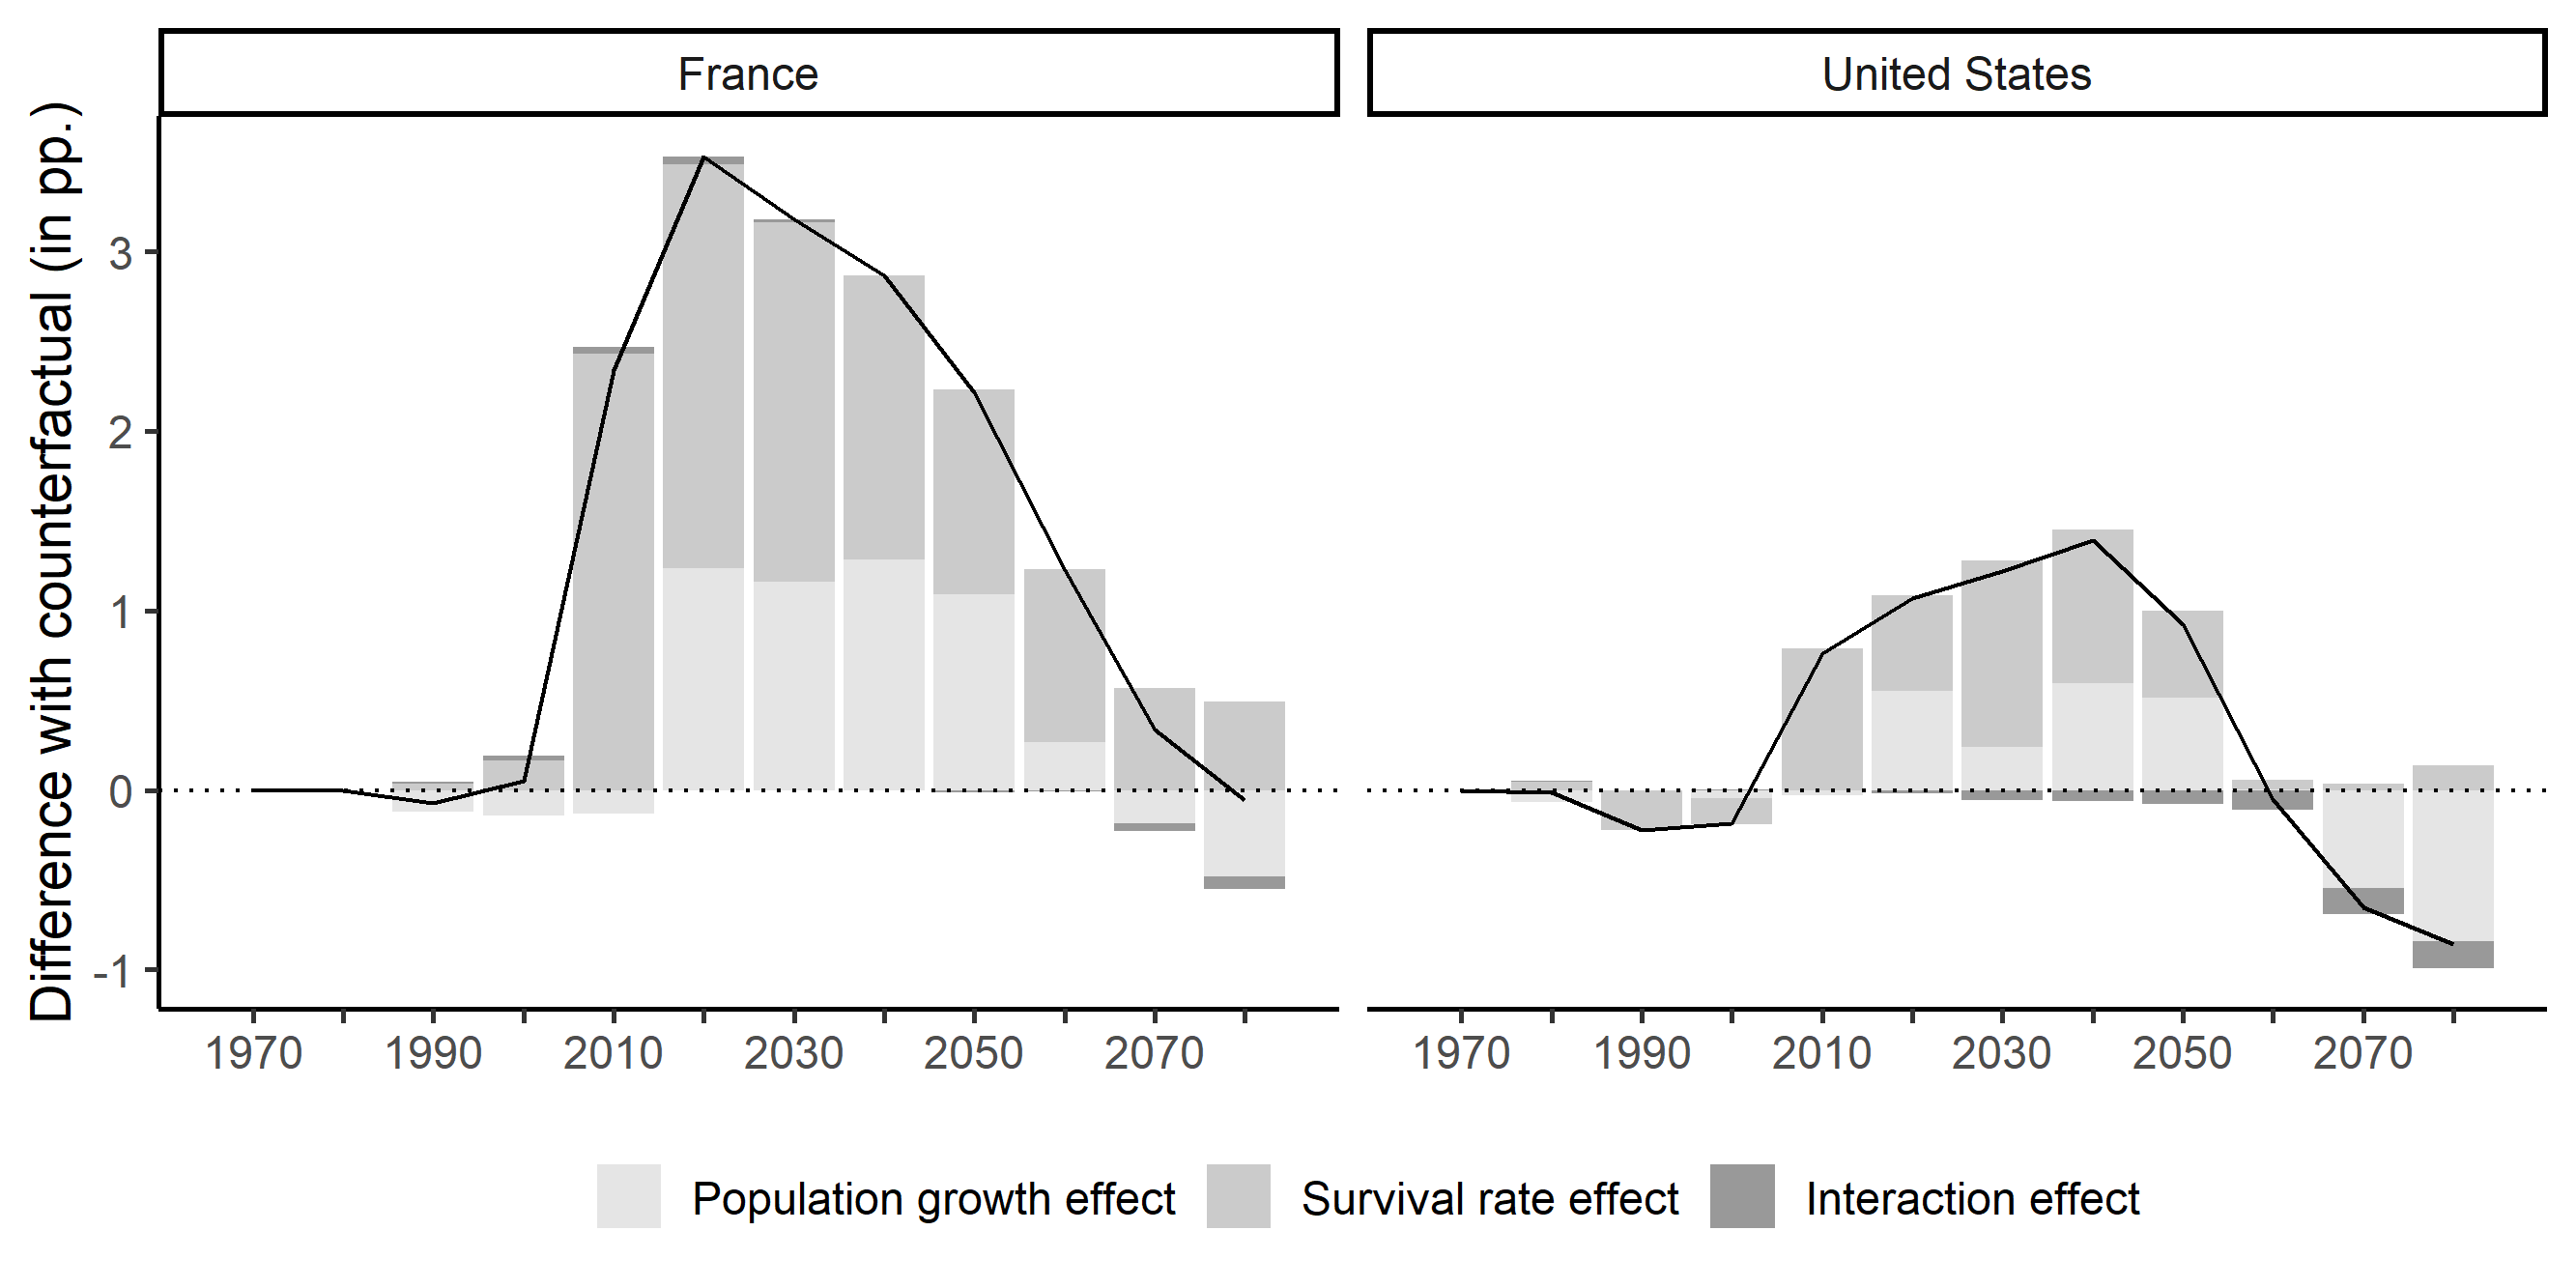
\includegraphics[width=1\linewidth]{../result/decomposition/decomp_PGSR.png}
	\caption{Aging-effect decomposition by determinants}
	\label{fig:decomp_PGSR}
	%	\vspace{.5ex}
	%	\hrule
	%	\vspace{-4ex}
	%	\justify\singlespacing\footnotesize 
\end{figure}
As mentioned above, the survival rate effect has kept the labor share relatively high in both countries. Another way to think about that is to consider demographic dynamics in terms of cohort sizes. Until 2010, if the survival rate had been held constant, then the massive increase in the population of young households due to the baby-boomers' presence would have generated an even larger decline of the labor share. However, the aging population (i.e. the increase of the survival rate) has thwarted part of this fall. Notice that the difference with the counterfactual is less than 1\% in the case of the United-States. It suggests that the aging phenomenon over this period is a larger determinant of the labor share in France compared to the United-States.
%After 2010, the explanation power of the survival rate falls and the distance between the benchmark simulation with respect to the counterfactual shrinks. It corresponds to the fact that demographic variations are not as wide as during the end of the 20th century.
The analysis of the determinants only reveals part of the explanation. It is also necessary to look at the channels that affect the labor share.

\subsubsection{Direct and indirect cohort effects}

To neutralize the indirect cohort effect, I fix the youth political weight $\eta_t$ to its 1970's value but I keep the demographic variables' time series $n_t$, $p_t$ and $p_{t+1}$ as in the benchmark simulation. Thus, $\eta_t = \eta_{1970}$. To neutralize the direct cohort effect, I assume that all the demographic variables remain at their 1970's level. Thus, $p_t = p_{1970}$, $p_{t+1} = p_{2010}$, $n_t = n_{1970}$ and population sizes but also initial capital stocks are recalculated. But the youth political weight time series $\eta_t$ is the one of the benchmark simulation. Finally, a last counterfactual is made where I neutralize both effects.\footnote{This last specification is the same as in the survival rate and population growth effects decomposition. So the purple curve in figure \ref{fig:counter_PGSR_1970}.}

Figure \ref{fig:counter_DEIE} displays the model predictions of the labor share with counterfactual specifications.
\begin{figure}[tb]
	\centering
	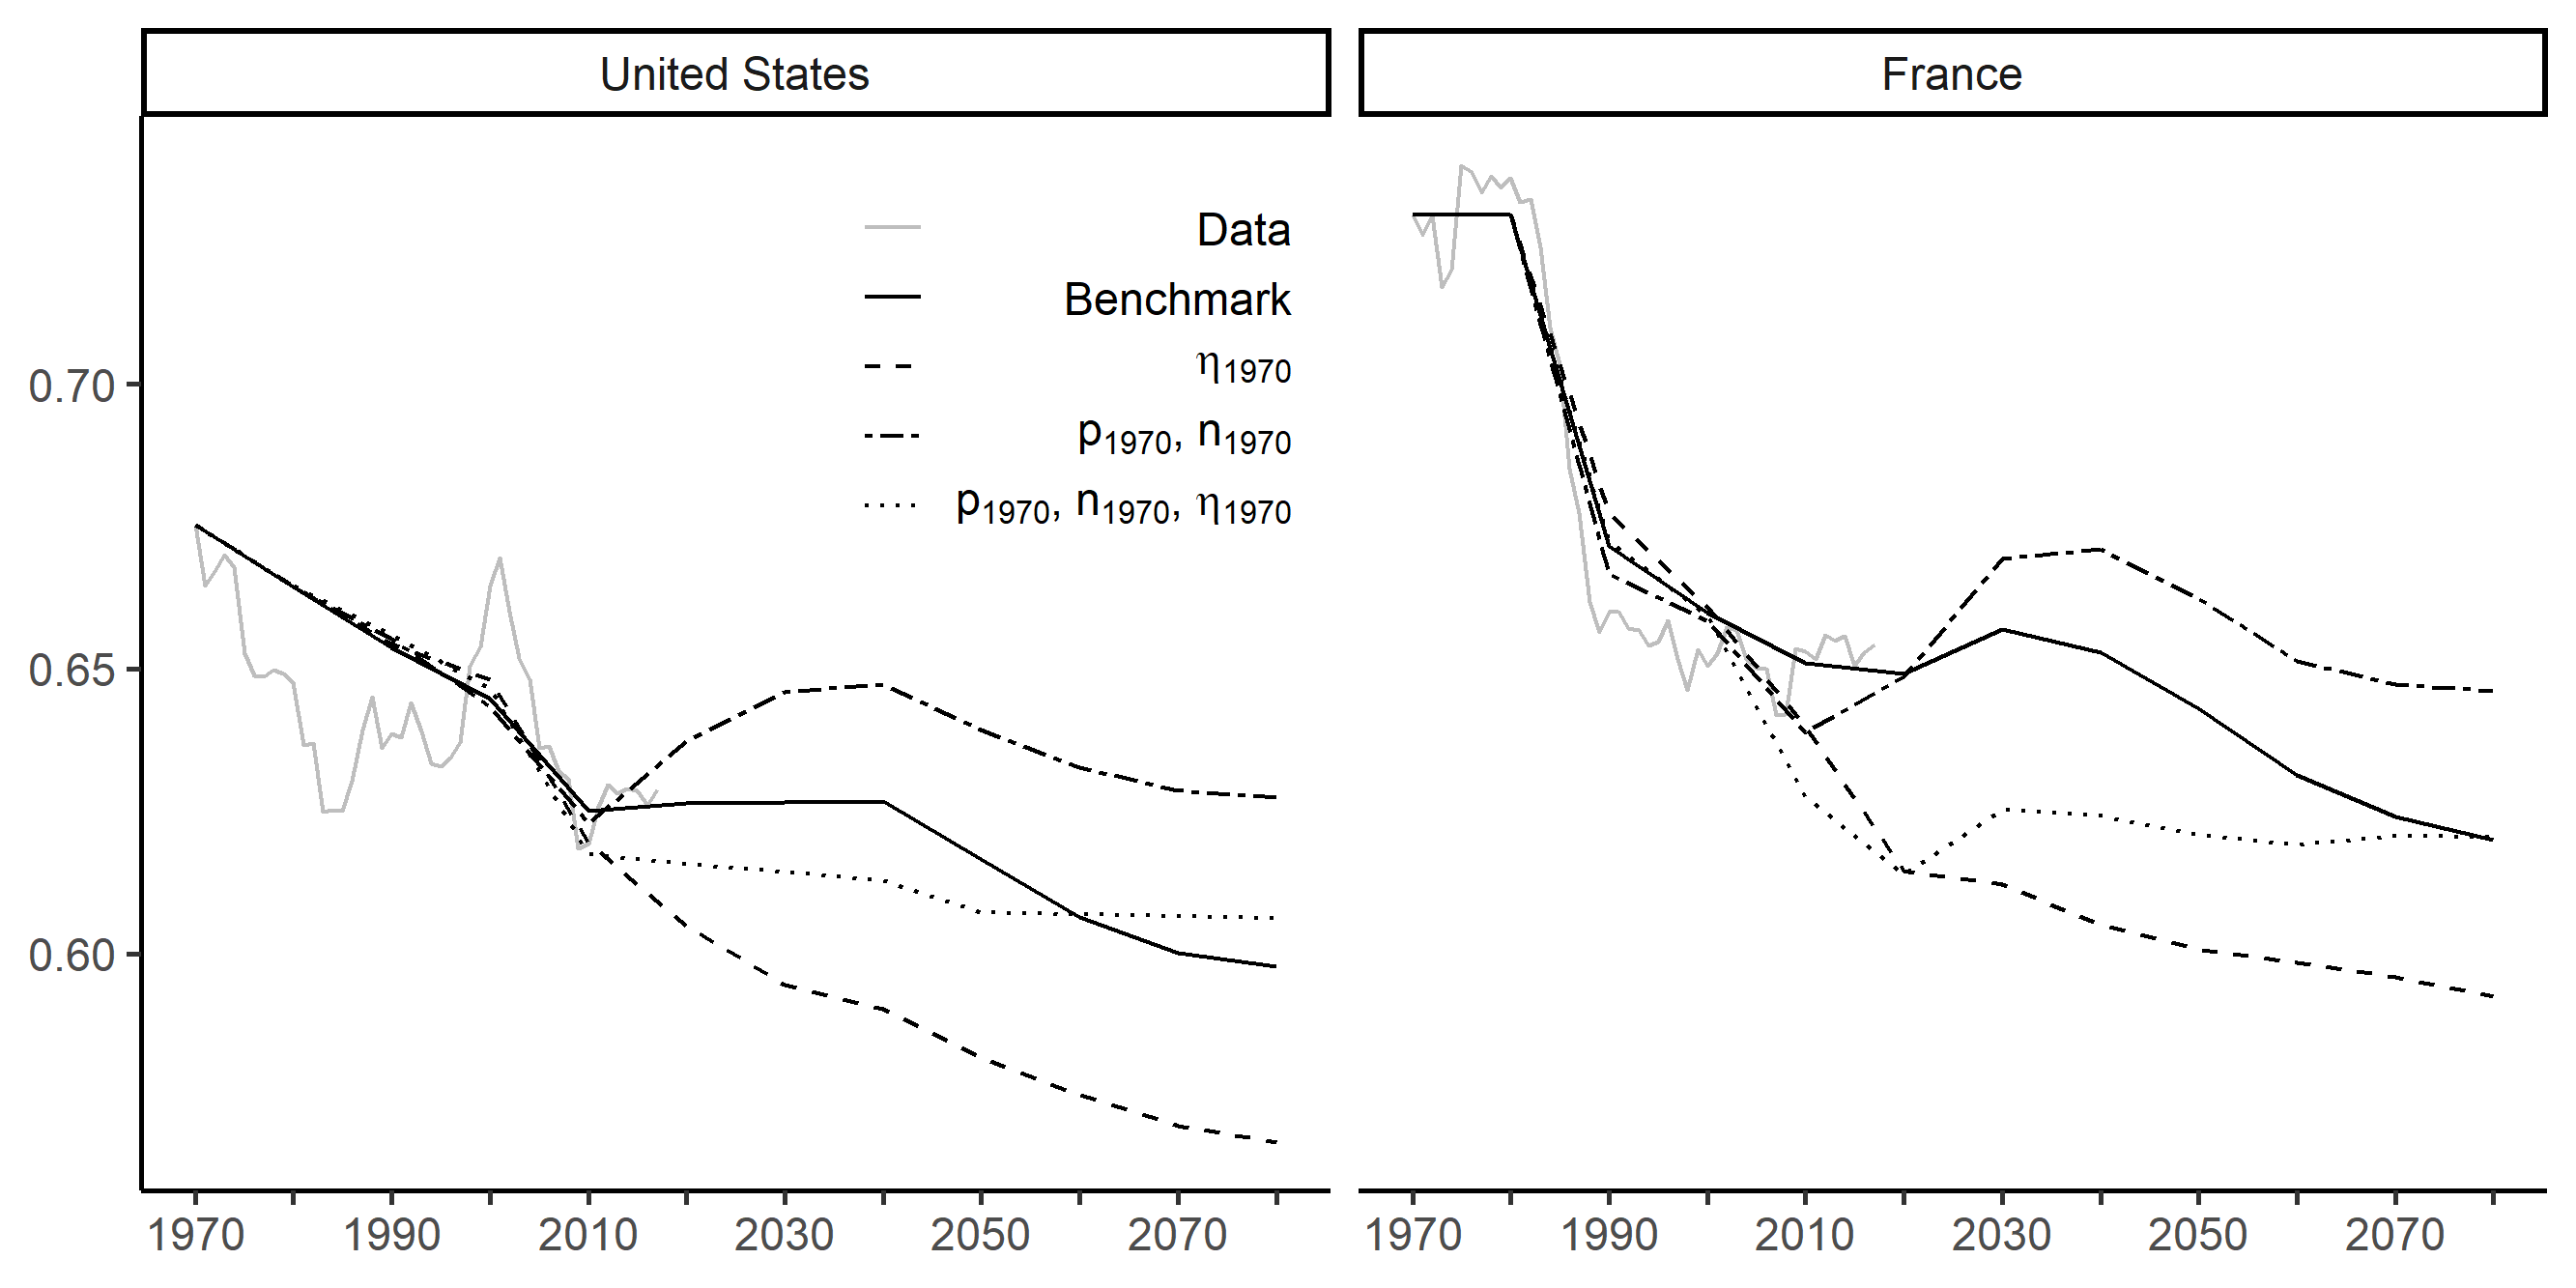
\includegraphics[width=1\linewidth]{../result/decomposition/counter_DEIE.png}
	\caption{Model predictions of the labor share with counterfactual specifications}
	\label{fig:counter_DEIE}
	%	\vspace{.5ex}
	%	\hrule
	%	\vspace{-4ex}
	%	\justify\singlespacing\footnotesize 
\end{figure}
The methodology to interpret this figure is similar to the one of the figure \ref{fig:counter_PGSR}. The dash-dotted curve corresponds to the direct cohort effect. For both countries, this curve is below the benchmark curve until 2010 and above thereafter. It means that the demographic dynamics' net impact through the direct channel is positive on the labor share until 2010 and negative thereafter. Looking at the dashed curve, it is slightly above before 2000 and largely below thereafter. The net impact of the indirect cohort effect is negative up to 2000 and positive subsequently. However, this representation is also tediously legible. Therefore, I isolate the extent of each channel with the same methodology as before. Figure \ref{fig:decomp_DEIE} displays the labor share's gap between the benchmark and the counterfactuals in percentage points.
\begin{figure}[tb]
	\centering
	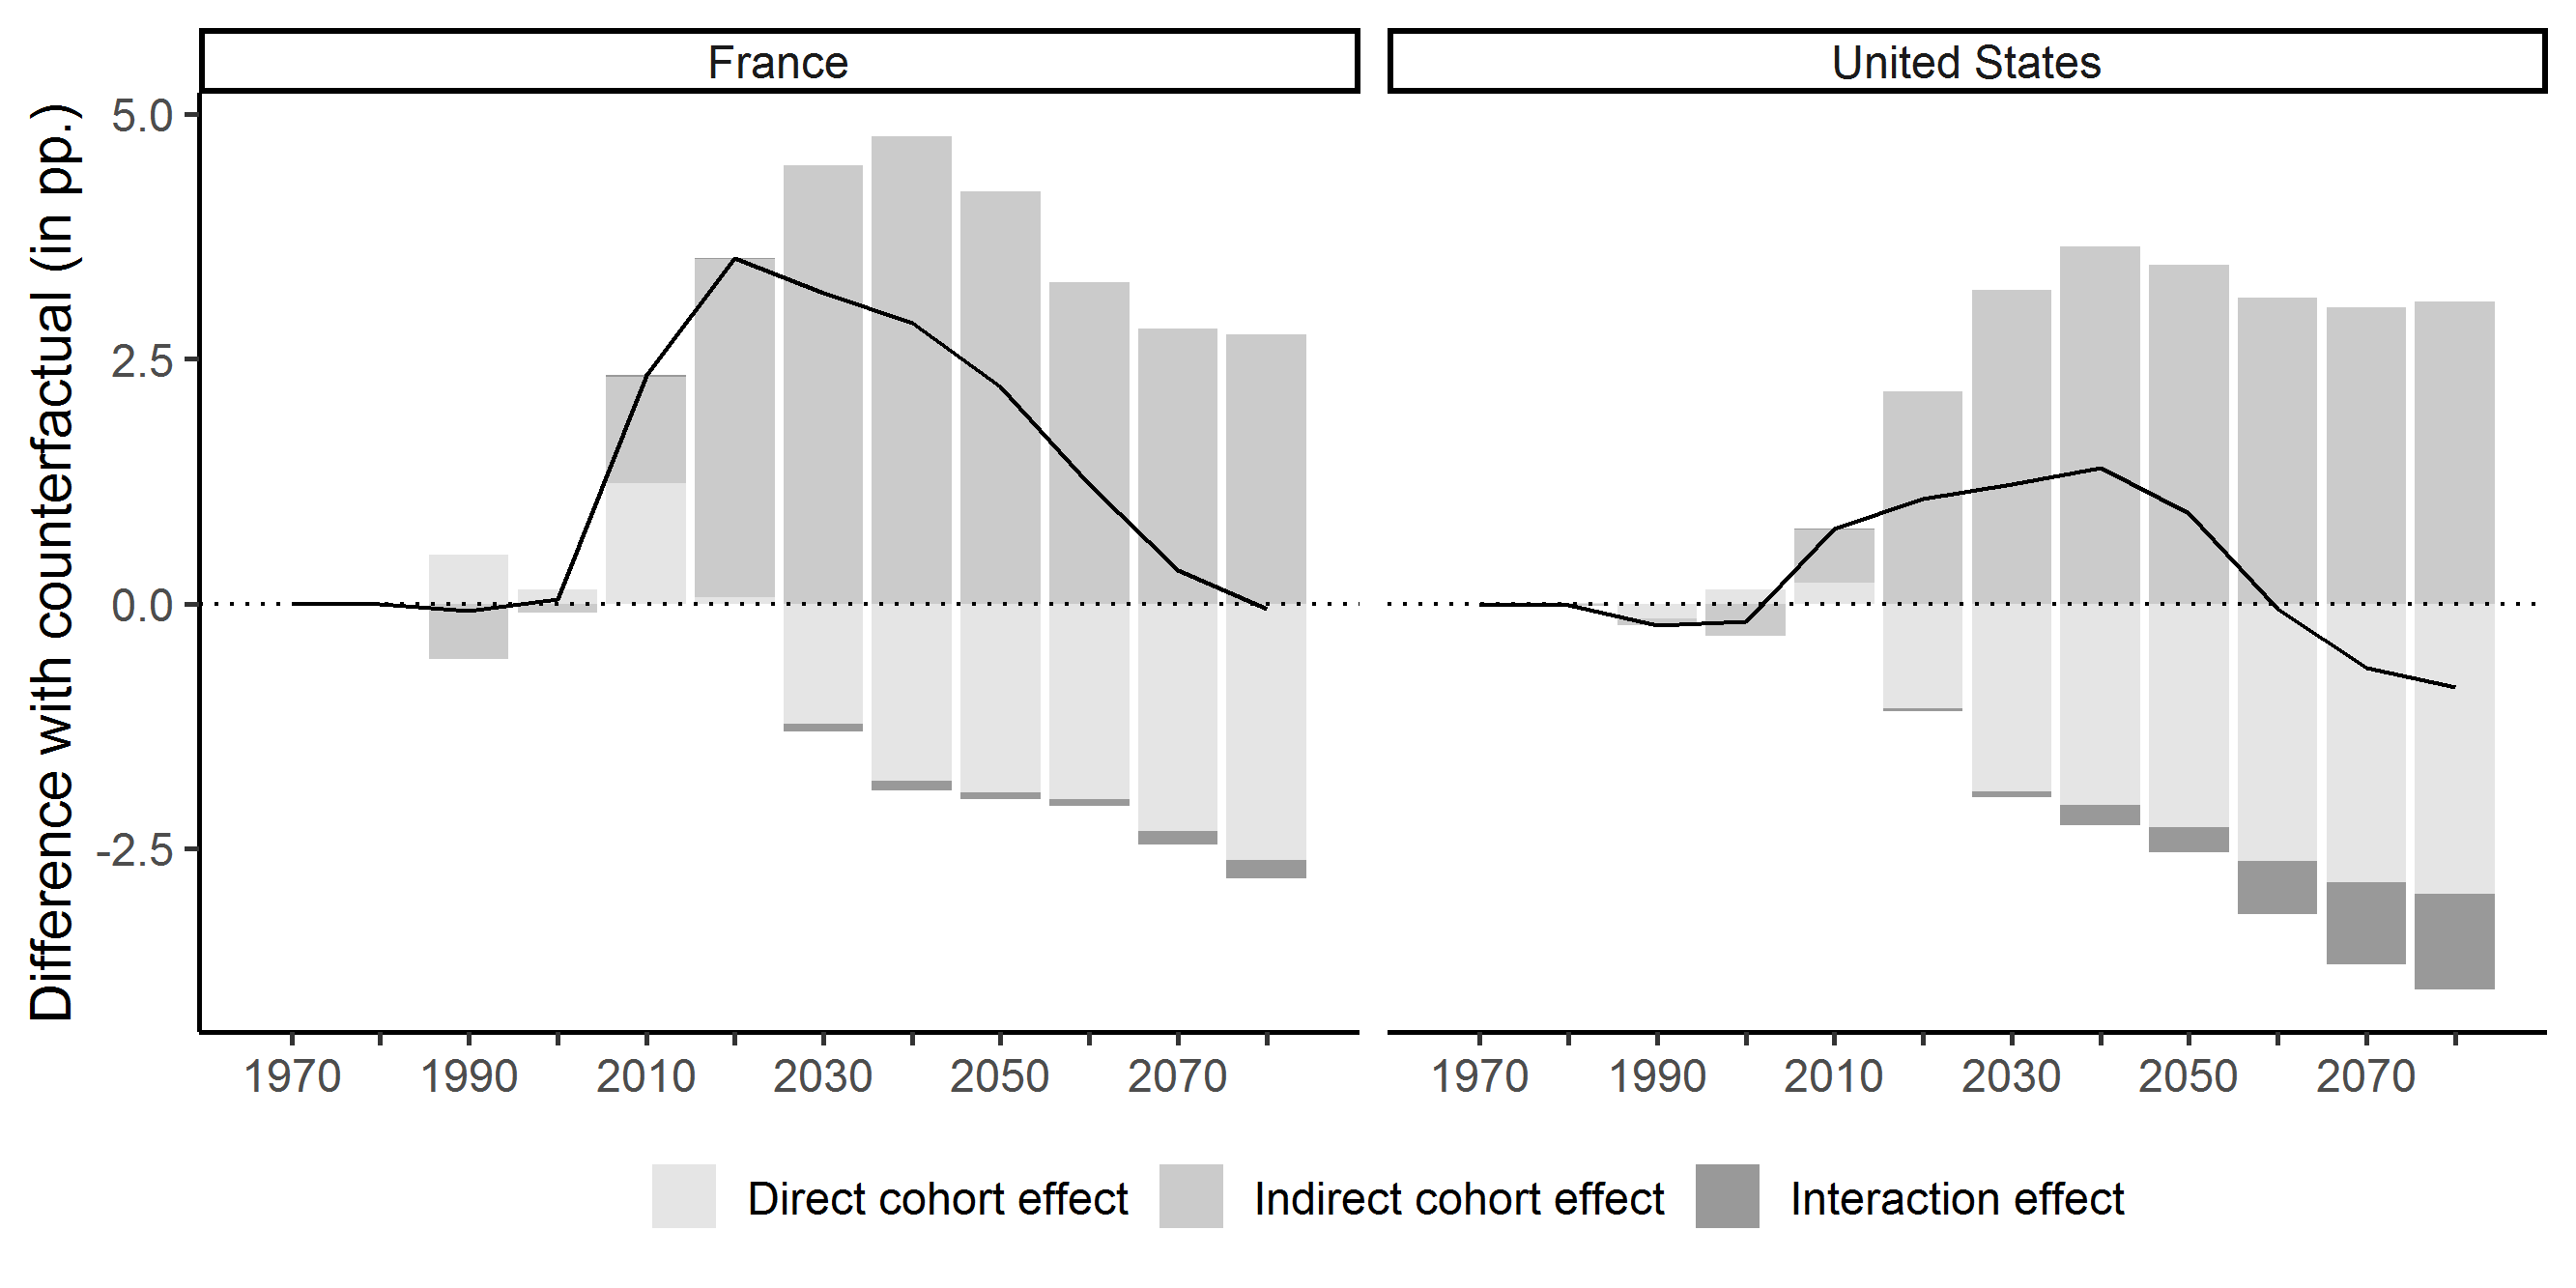
\includegraphics[width=1\linewidth]{../result/decomposition/decomp_DEIE.png}
	\caption{Aging-effect decomposition by channels}
	\label{fig:decomp_DEIE}
	%	\vspace{.5ex}
	%	\hrule
	%	\vspace{-4ex}
	%	\justify\singlespacing\footnotesize 
\end{figure}
The direct cohort effect is positive when the baby-boomers are young and after becomes negative. While the indirect cohort effect has the opposite pattern. The direct cohort effect dominates the indirect one until 2010 before to become less influential. Until 2010, if the demographic variables had been held constant, then the relatively high political power of the youth due to the baby-boomers' presence would have generated an even larger decline of the labor share. However, the aging population was mainly driven by the increasing survival rate which has thwarted part of the fall. Notice that, here again, the difference with counterfactual is less than 1\% in the case of the United-States. It suggests that the aging phenomenon over this period is a larger determinant of the labor share in France compared to the United-States.
% May be for the Summary
After 2010, so once the baby-boomers' cohort retires, the model predicts that the indirect cohort effect (i.e. the decline of the youth political power) should exceed the direct one. This is directly related to the mechanism analysis of section \ref{subsec:model_pred}. The baby-boomers and more generally the old households becomes the winners of the age-related conflict within the public policy over this period. Thereby, they reduce the workers' outside option which leads to a wage cut or more precisely to a wage stagnation. The labor cost remains constant while the capital available in the economy accumulates. It generates an incentive for the representative firm to hire more workers. As a result, the labor share increases.
% May be for the Summary

\subsubsection{Summary}

Figure \ref{fig:decomp_country_period} summarizes the aging-effect decomposition by periods and countries.
\begin{figure}[tb]
	\centering
	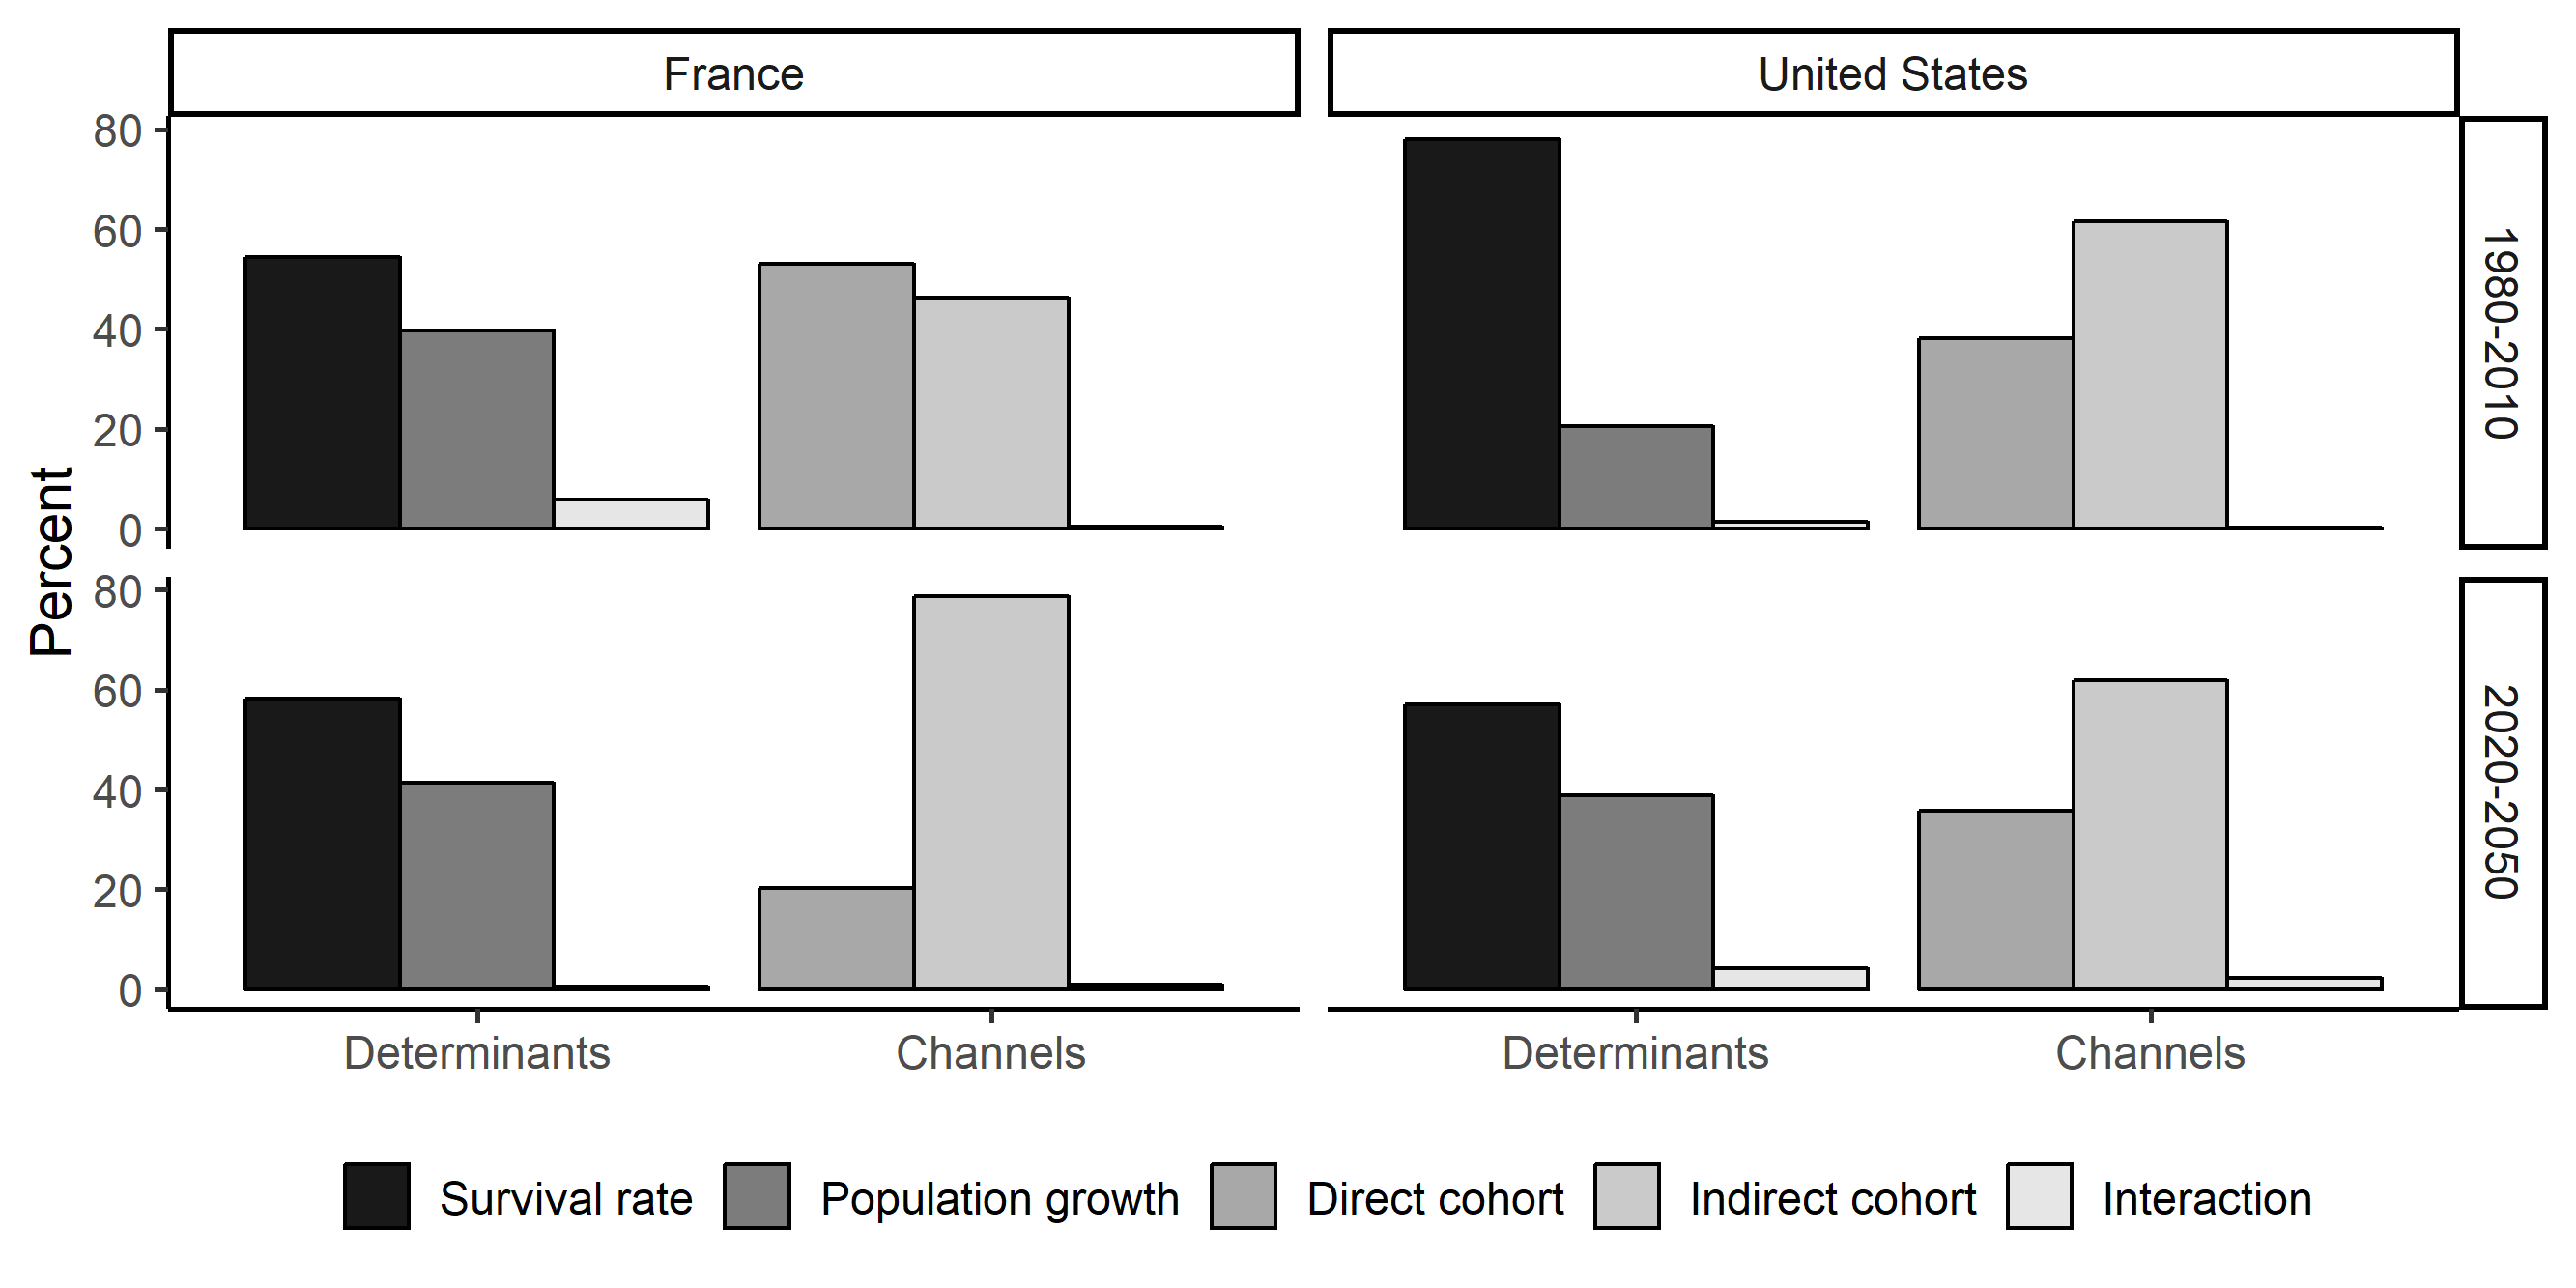
\includegraphics[width=1\linewidth]{../result/decomposition/decomp_country_period.png}
	\caption{Aging-effect decomposition by periods and countries}
	\label{fig:decomp_country_period}
	%	\vspace{.5ex}
	%	\hrule
	%	\vspace{-4ex}
	%	\justify\singlespacing\footnotesize 
\end{figure}
Both countries have almost similar patterns. The main determinant of the aging phenomenon is the survival rate. On average, it explains 54.5\% for France and 78.1\% for the United-States of the impact on the labor share over the period 1980-2010. This decomposition persists thereafter. However, the channel decomposition does not. Between 1980 and 2010, demographic dynamics affect the labor share mainly through the direct channel in France. While the indirect one is dominant in the United-States. On average, the share explained by the direct cohort effect is about 53.1\% for France and 38.2\% for the United-States. However, over the next period, the direct cohort effect is not the dominant channel anymore in France. It falls down to 20.3\%. It suggests that the indirect cohort effect becomes the main carrier of the demographic dynamics on the labor share. While it remains relatively stable in the United-States around 35.7\%.




	
	\section{Discussion} \label{sec:discussion}
	% Introduction of the discussion


% May move this subsection to the discussion.
\subsection{Age-related conflict : who are the winners ?}

So far, the labor share has been declining due to the baby-boomers generation in both countries. First, when they were young because they shaped the public policy and so the labor market institutions in their favor. The firms answered to that by substituting labor to capital. Second, when they were old because they have considerably increased the available capital in the economy through savings allowing the firms to substitute even more. However, the labor income share is a gross indicator of inequalities. A more appropriate indicator may be the income ratio between young and old after redistribution. 

From equation \eqref{eq:after_tax_income_ratio}, I have that the after-tax young-to-old income ratio is equal to the young political weight (i.e. $Y_t^y/Y_t^o = \eta_t$). While the before-tax young-to-old income ratio corresponds to the labor-to-capital ratio (i.e. $\Theta_t = \frac{w_tL_t}{r_tK_t}$). Figure \ref{fig:raw_vs_net_inc_ratio} displays these income ratios in deviation from the 1970 steady-state.
\begin{figure}[tb]
	\centering
	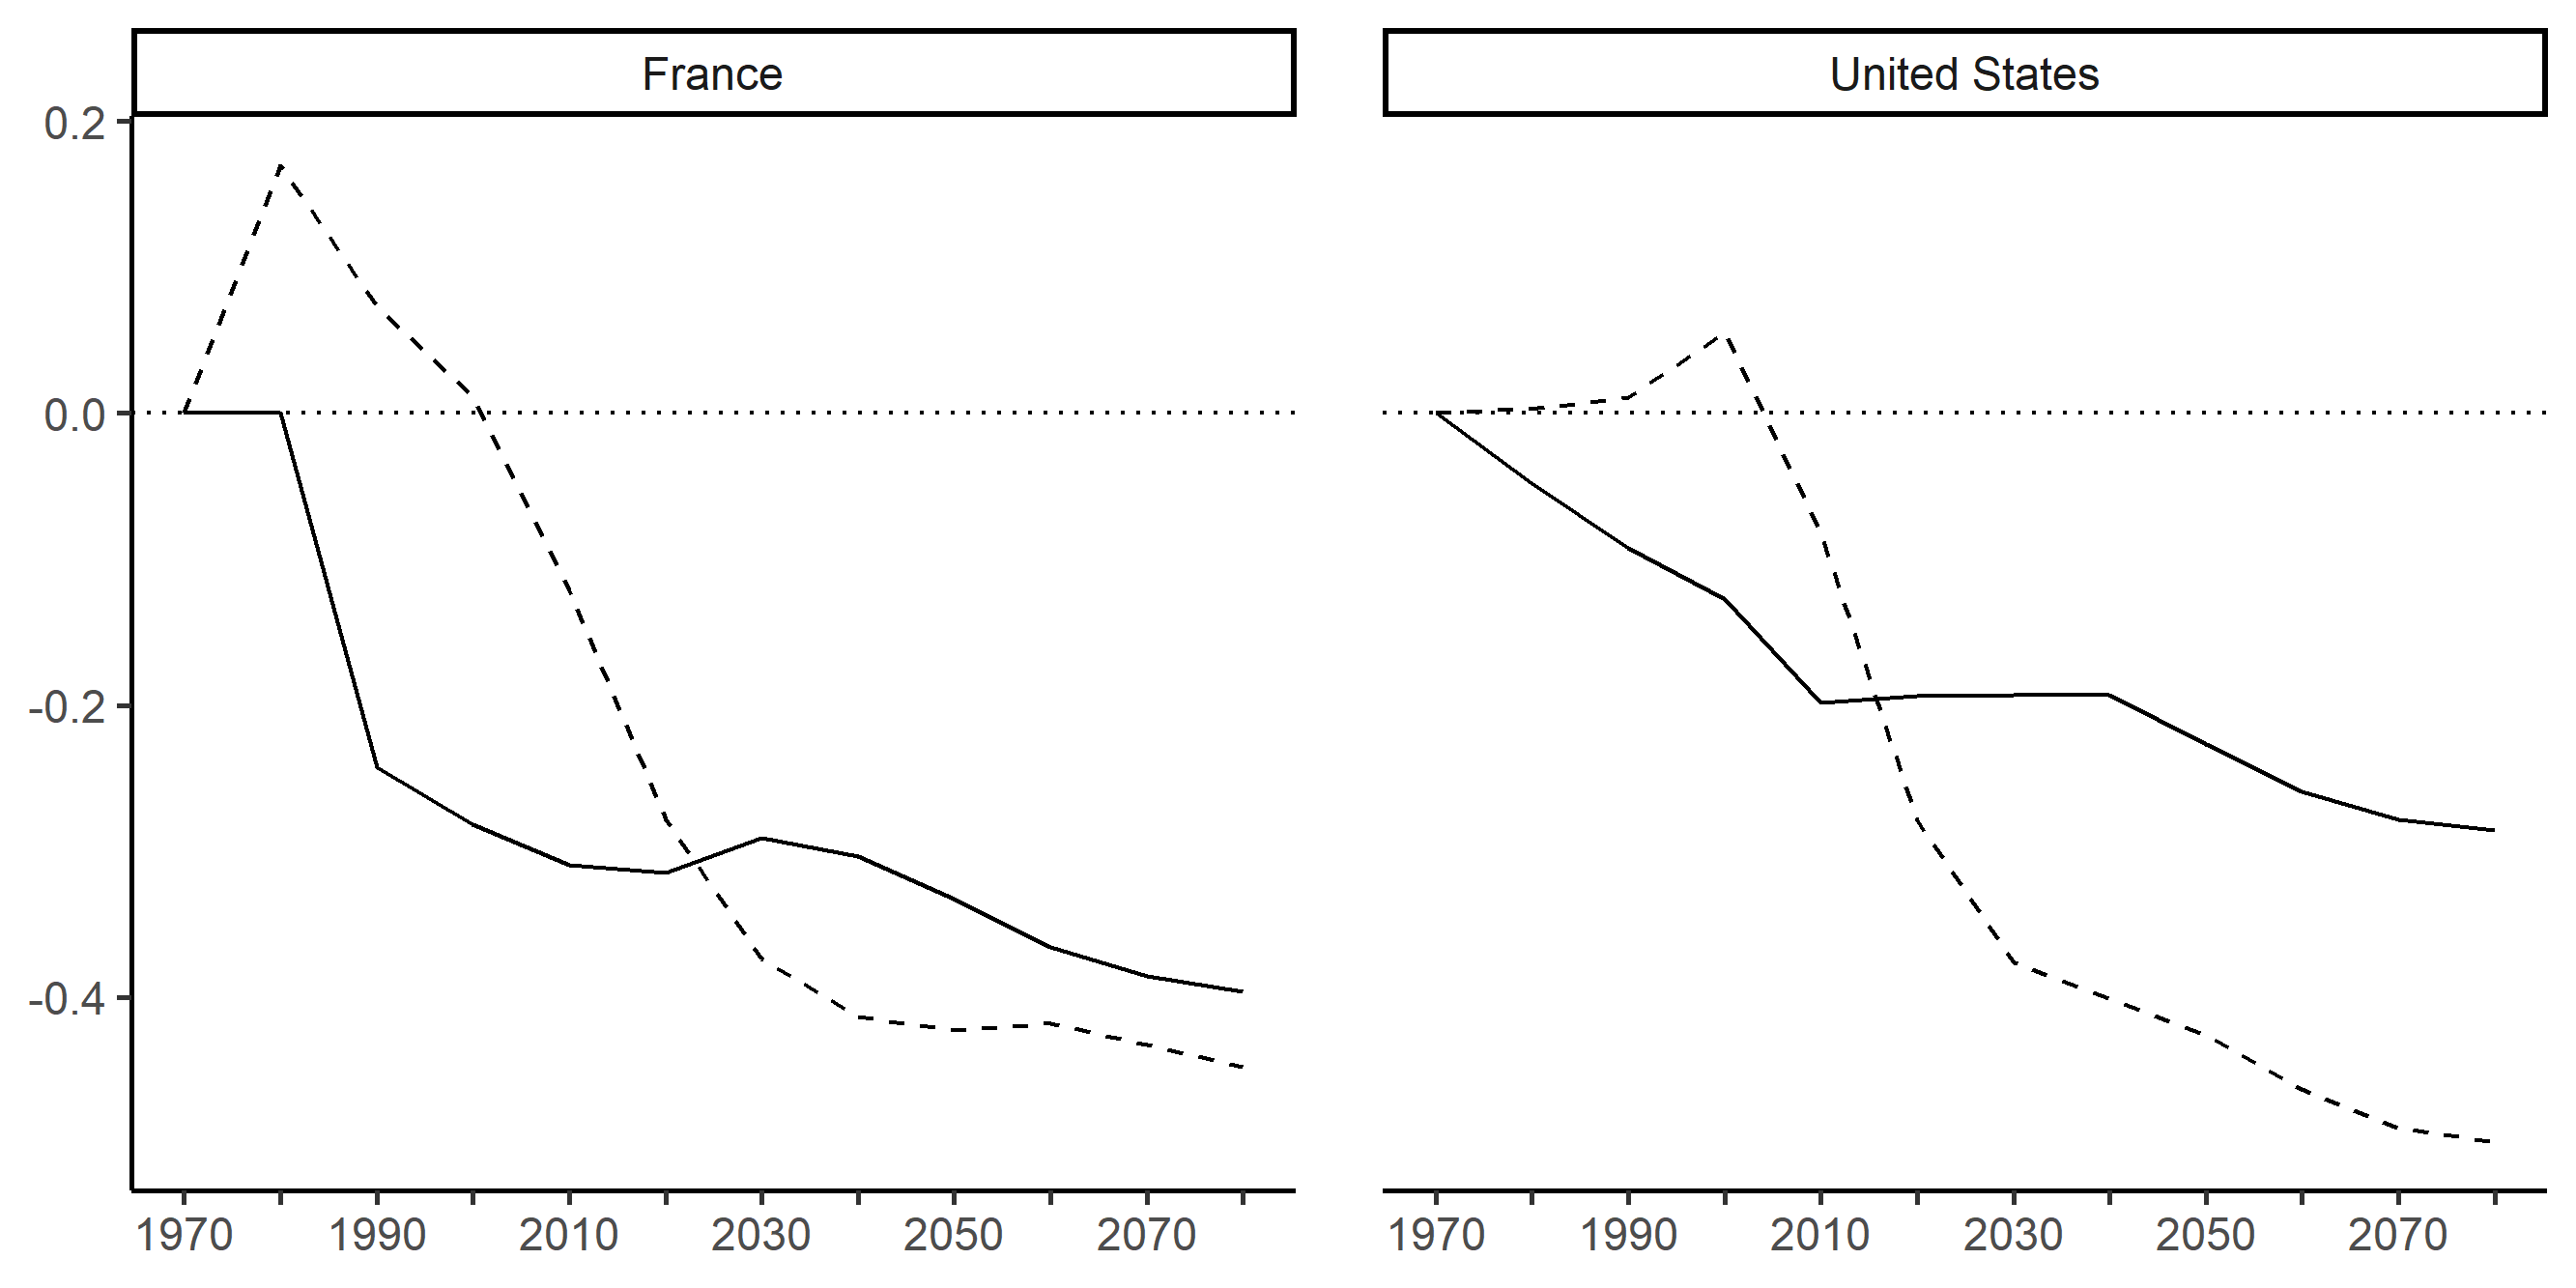
\includegraphics[width=1\linewidth]{../result/redistribution/dev_incratio_raw_vs_net.png}
	\caption{Deviation from the 1970 steady-state of the before-tax (solid) and after-tax (dashed) young-to-old income ratios}
	\label{fig:raw_vs_net_inc_ratio}
	\vspace{.5ex}
	\hrule
	\vspace{-4ex}
	\justify\singlespacing\footnotesize The solid line corresponds to the before-tax young-to-old income $\Theta_t$ ratio also named the labor-to-capital income ratio $\frac{w_tL_t}{r_tK_t}$ and the dashed line is the after-tax young-to-old income ratio $Y_t^y/Y_t^o$. Deviation is expressed in percentage.
	% and the dotted line is the after-tax young-to-old income ratio with government health spending included in old households income $Y_t^y/(Y_t^o+h_tN_t^o$).
\end{figure}
While the labor share and so the labor-to-capital ratio (i.e. before-tax young-to-old income ratio) sharply decline between 1970 and 2000, the after-tax young-to-old income ratio lies over its 1970's level during the same period. Even if I include the government health spending as part of the old households income, the young-to-old income ratio remains over its initial level until 2000.\footnote{In terms of deviation, the curve is combined with the dashed one.} This model prediction holds for both countries. The baby-boomers gross income share (i.e. labor income share) has declined due to the mechanisms previously mentioned when they were young. However, they also have spurred political parties to implement redistributive public policies.\footnote{This is the result of the probabilistic voting specification. The opportunist behavior of political parties lead them to favor this generation in order to maximize their probability to win the election.} This redistribution is characterized, in terms of the model, through a raise of the tax rate and an increase of the unemployment spending share within the government revenue.\footnote{Notice that the increase of the unemployment spending share is driven and accentuated by the raising unemployment due to factor substitution.} Thus, they have been able to seize part of their elders income through redistribution. Even though baby-boomers appeared has income losers over this period because the labor share was falling, they are actually the winners once net income is considered.

Another way to determine the winners of the age-related conflict within the public policy is to look how the GDP is split. Figure \ref{fig:inc_gdp_shr} displays the income allocation after redistribution.
\begin{figure}[tb]
	\centering
	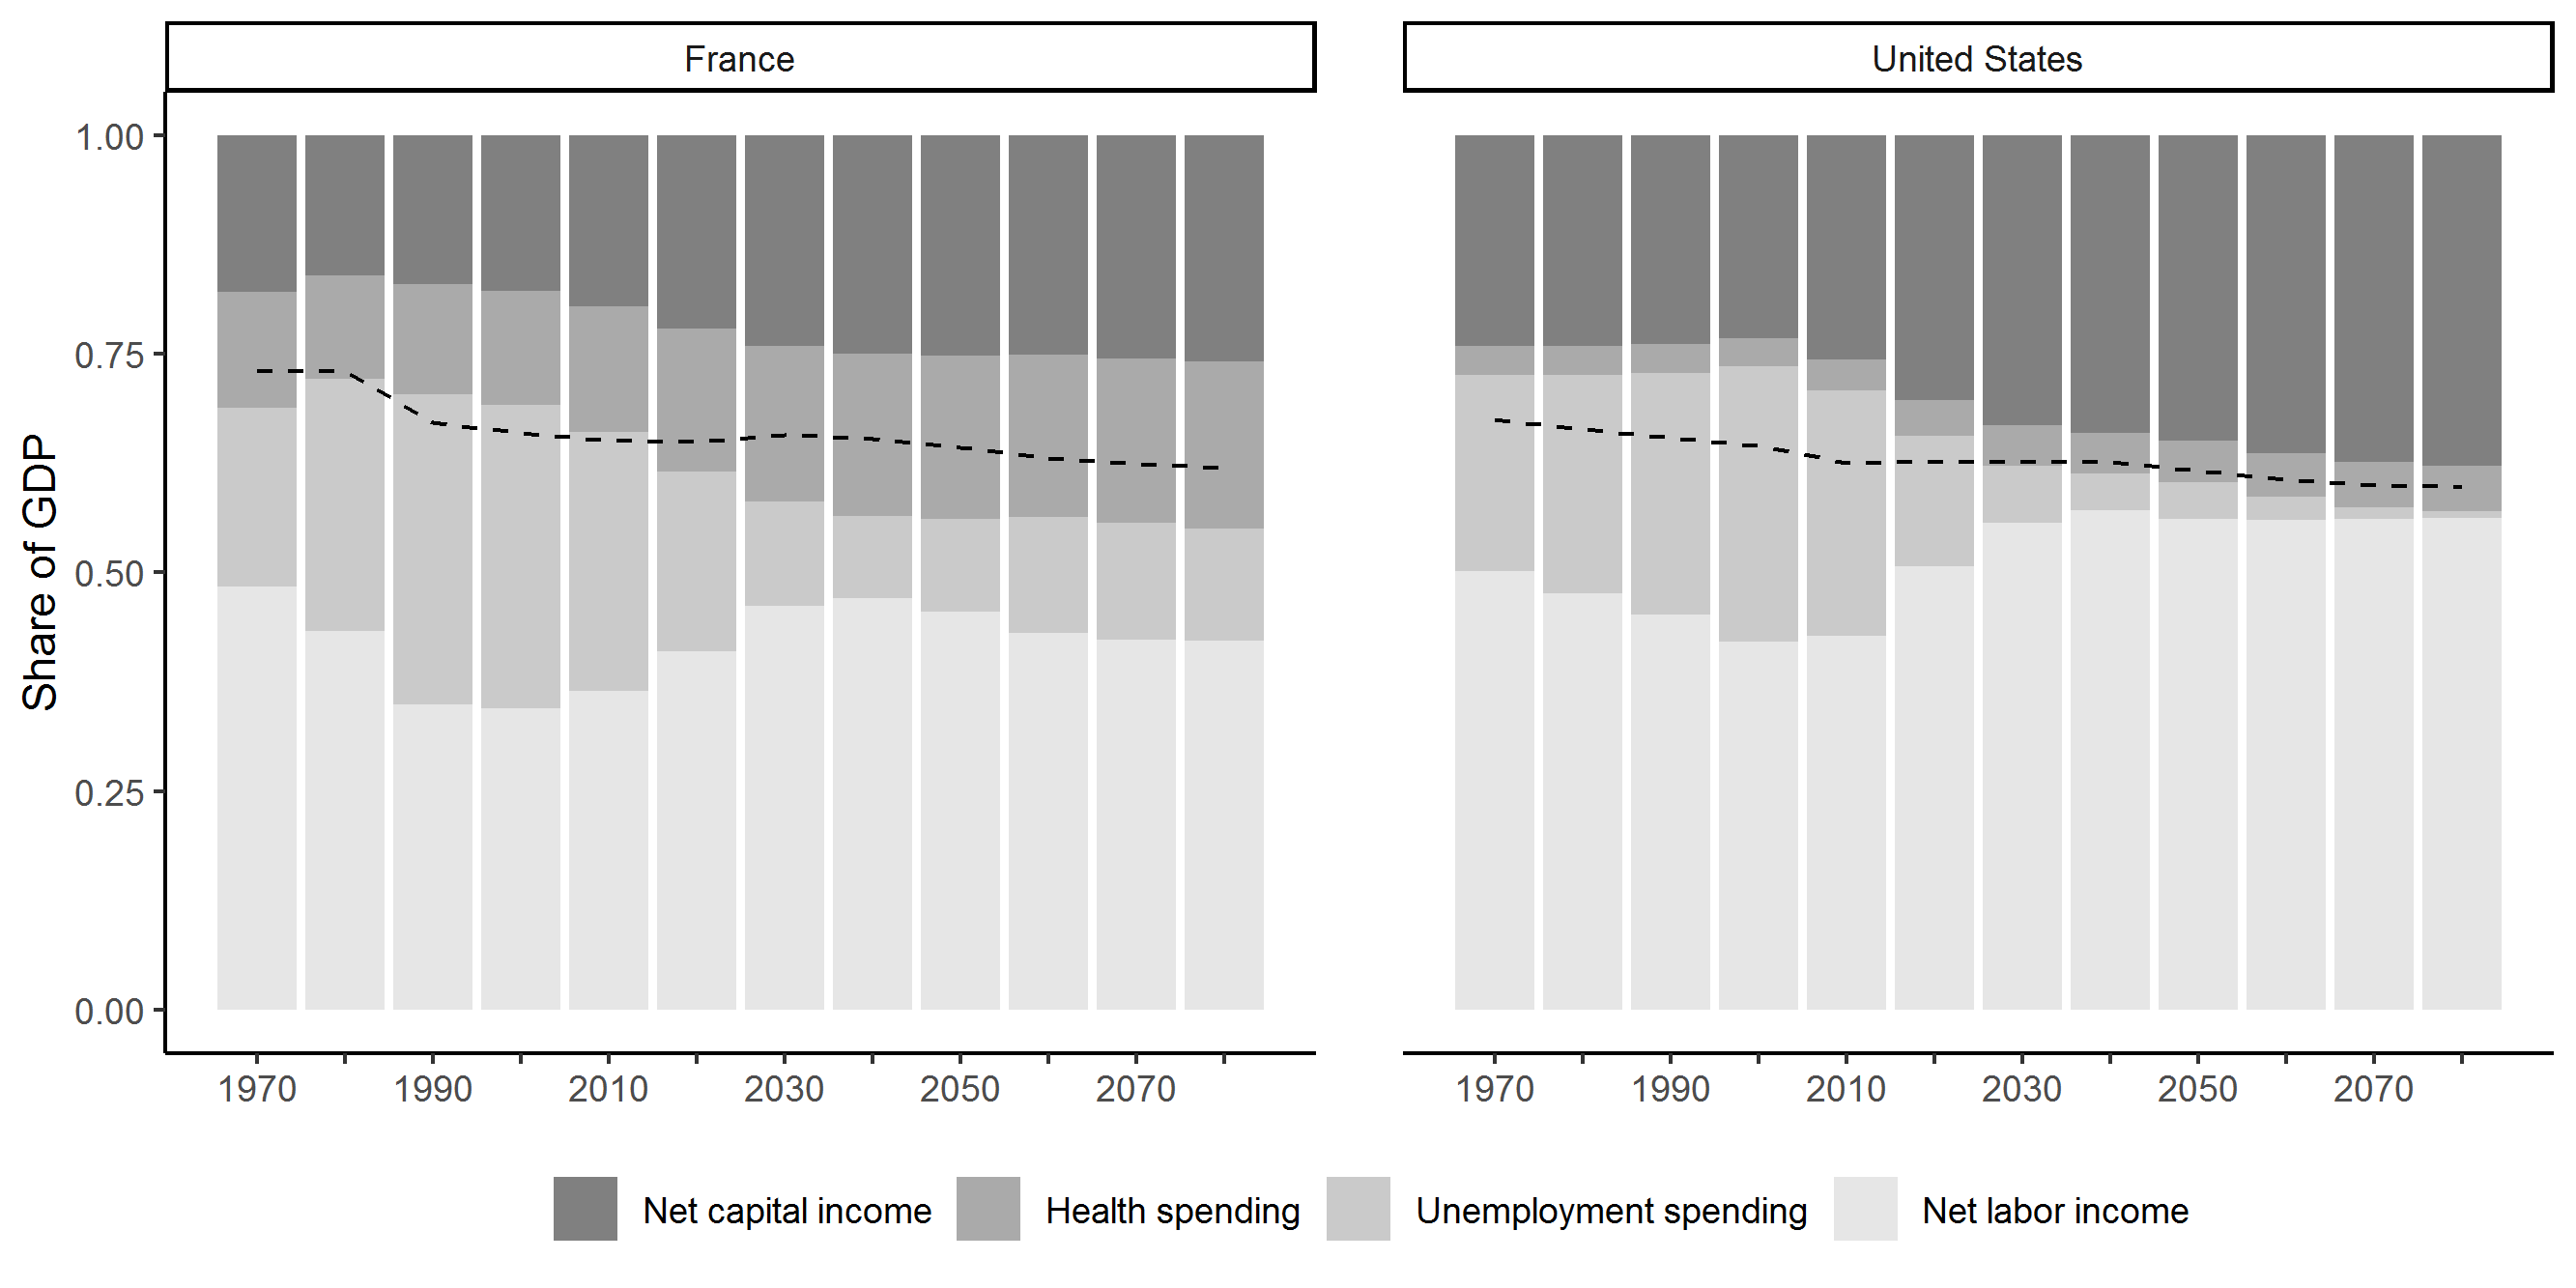
\includegraphics[width=1\linewidth]{../result/redistribution/redis_step3_stacked.png}
	\caption{After-tax income share allocation}
	\label{fig:inc_gdp_shr}
%	\vspace{.5ex}
%	\hrule
%	\vspace{-4ex}
%	\justify\singlespacing\footnotesize The dashed black line corresponds to the labor share, so the before-tax young income share.
\end{figure}
The dashed black line corresponds to the labor share, so the before-tax young income share. As long as this curve lies in the purple area (i.e. government unemployment spending share), it means that old agents fund unemployment spending through their taxes. On the contrary, when this curve lies in the orange area (i.e. government health spending share), the young agents fund government health spending for their elders. The US share of GDP which is allocated to health spending is quite small compared to the French one. This is directly related to the preference parameter for government health spending $\beta$.\footnote{$\beta_{\text{FR}} = 0.739$ and $\beta_{\text{US}} = 0.138$.} The US young generations are the winners of the age-related conflict from 1970 to 2020 which corresponds to the active period of the baby-boomers. Once the US population ages and therefore the baby-boomers, old households dominates the public policy conflict. However, the size of the government revenue declines due to the fact that the United-States converges to full employment in the long run. For France, the baby-boomers also dominate the public policy conflict between 1990 and 2010 when they are active. Once they retire, so over the period 2010-2040, they are still the winners of this conflict and their children fund government health spending. Notice that the size of the welfare state corresponds to the sum of the unemployment benefits share in GDP and the health spending share in GDP.

\subsection{Retirement age}

So far, I have not discussed the retirement age and its implications on the labor share.
% Literature on the impact of the retirement age on growth / Futagami and Nakajima (2001) / Gonzalez-Eiras and Nieplet (2012) / ?
As mentioned in the introduction, the relationship between aging and economic growth has received much more attention than the one with the labor share. \cite{Gonzalez-Eiras2012} predict that the retirement age in OECD countries should increase in response to population aging. In their model of politico-economic equilibrium, individuals vote with perfect foresight and decide to raise retirement age as long as population ages. Agents work longer and so accumulate more wealth, it reduces social-security transfers and thereby releases more government spending to public investment which is an engine for growth.\footnote{However, this result contrasts with \cite{Jager2016} who find out that the share of elderly people and public investment are negatively co-integrated. They use panel data of 19 OECD countries from 1971 to 2007. This gap may be due to two reasons: \textit{i)} some public policy instruments which are not considered in the model of \cite{Gonzalez-Eiras2012} might invert the relationship between aging and public investment; \textit{ii)} the perfect foresight assumption might be too strong. Both potential explanations may reconcile these diverging results.} On the contrary, \cite{Futagami2001} claim that population aging does not necessarily depress economic growth and may even foster it through savings. Thus, postponing the retirement age would result in a decline of savings and so the economic growth. \cite{Dedry2017} also discuss the role of legal retirement age according to the type of pension system in a context of population aging due to either declining fertility or increasing longevity.

In order to take into account the role of retirement age, I perform counterfactual predictions with different scenarii based on an exogenous change. The retirement age is captured within the variable $p_t$ which depends negatively on it but positively on the life expectancy. I do not endogenize this variable due to the limited form of rationality and to the several assumptions that would be required.\footnote{To have an endogenous retirement age, agents should vote on it and thereby vote on the survival rate. The first question would be to determine whether agents vote on $p_t$, $p_{t+1}$ or both. Then, the perfect annuity market would have a lot of implications on the results. Since savings of young agents who die before reaching old age are distributed among their surviving peers, it means that an agent has an incentive to vote for a decline of the survival rate because fewer peers would reach old age. Thus, it would increase its income and so its utility. Therefore, it would be necessary to determine whether or not agents internalize the perfect annuity market in their voting decisions.} In the public debate, it is often argued that the legal retirement age should change in the future, usually upward, as claimed by \cite{Gonzalez-Eiras2012}% \textbf{(more/other references)}.
. Between 2020 and 2030, I suppose a positive exogenous shock on the age of retirement. Meaning that less individuals would reach the old age which is translated into a decline of the survival rate, i.e. $p_t$. As in section \ref{subsec:counterfactual}, other demographic variables have to be changed for the period following the shock of each simulation's sequence (i.e. 2030, 2040, 2050 and 2060). However, the implications for demographic dynamics are not identical to this previous exercise. Because the greater the retirement age, the longer an individual remains young in terms of the model. Thus, these individuals do not vanish but just remain longer in the labor force.\footnote{In the same way, the capital stock of these periods is not changed as in section \ref{subsec:counterfactual} because it has already been accumulated through savings from previous periods. It has no reason to vanish or to be scraped.}
The logic is the same as the law of conservation of mass from A. Lavoisier: ``\textit{nothing is lost, nothing is created, everything is transformed}''.
Therefore, conjointly with the decline of the survival rate, there is a share of the young population that does remain young.
From the identity $\frac{N_t^o}{N_t^y} \equiv \frac{p_t}{n_t}$, I obtain:
\begin{equation} \label{eq:demo_growth_identity}
	\frac{\dot{N}_t^o}{N_t^o} - \frac{\dot{N}_t^y}{N_t^y} = \frac{\dot{p}_t}{p_t} - \frac{\dot{n}_t}{n_t}
\end{equation}
where the upper dotted variables correspond to the variables' variation, e.g. $\dot{N}_t^o = {N_t^o}^\prime - N_t^o$ where ${N_t^o}^\prime$ is the new value for $N_t^o$. This equation has to be satisfied. The exogenous shock on $p_t$ affects all other demographic variables. Firstly, the size of the old population varies as much as the survival rate does, i.e. $\frac{\dot{N}_t^o}{N_t^o} = \frac{\dot{p}_t}{p_t}$. Secondly, the variations of the young population's size are inversely proportional to the ones of the old population size, i.e. $\frac{\dot{N}_t^y}{N_t^y} = -\frac{\dot{N}_t^o}{N_t^o}$. Thirdly, by taking into account the two previous points and the fact that equation \eqref{eq:demo_growth_identity} has to be satisfied, it implies that $\frac{\dot{n}_t}{n_t} = -\frac{\dot{p}_t}{p_t}$. Therefore, the exogenous shock on $p_t$ affects the other variables with the same magnitude.
% \footnote{To be more precise, the magnitude of the shocks on $N^y_t$ and $n_t$ should decrease over time.}
Hence,
\begin{align*}
	\dot{N}^o_t = \frac{\dot{p}_t}{p_t} N^o_t \implies& {N^o_t}^\prime = \left(1+\frac{\dot{p}_t}{p_t}\right) N^o_t \\
	\dot{N}^y_t = -\frac{\dot{p}_t}{p_t} N^y_t \implies& {N^y_t}^\prime = \left(1-\frac{\dot{p}_t}{p_t}\right) N^y_t \\
	\dot{n}_t = -\frac{\dot{p}_t}{p_t} n_t \implies& {n_t}^\prime = \left(1-\frac{\dot{p}_t}{p_t}\right) n_t
\end{align*}
where $\frac{\dot{p}_t}{p_t} = \frac{p^\prime_t - p_t}{p_t} \implies p^\prime_t = p_t + \dot{p}_t$. Thus, the new demographics variables $N^{o\prime}_t, N^{y\prime}_t, p^\prime_t, n^\prime_t$ are computed for the years 2030, 2040, 2050 and 2060. For the years 2070 and 2080: $n^\prime_t$ follows the benchmark time series and population sizes are computed with $N^{o\prime}_t = p^\prime_t {N^{y\prime}_{t-1}}$ and $N^{y\prime}_t = n^\prime_t N^{y\prime}_{t-1}$. Notice that new values of the expected survival rate $p^\prime_{t+1}$ changes according to $p^\prime_t$. Moreover, $\eta^\prime_t = \frac{n^\prime_t}{p^\prime_t}\frac{1+\alpha p^\prime_{t+1}}{\omega}$ is also recomputed.

Two types of scenario are possible for a change in the age of retirement between 2020 and 2030. Firstly, I consider that the retirement age increases in such a way that the survival rate is negatively affected by 10\% in 2030.\footnote{The underlying (strong) assumption of this whole exercise is that the change in retirement age has no consequences on life expectancy. Some authors argue that increasing the retirement age has a negative impact on health and so the life expectancy (see, for example, \cite{Insler2014} for the United-States; \cite{Coe2011} for Europe). Thereby, the negative effect on the survival rate may be all the more tenacious due to the declining life expectancy. Despite the presence of a potential co-integration of the retirement age and the life expectancy, I believe that the qualitative impact is not affected in the sense that the simulation is a lower bound.} Thereafter, the survival rate grows at the same growth rate as in the benchmark simulation.\footnote{I assume that the shock does not change the future growth path of the survival rate.} This first scenario can be summarized as a one-shot shift by 10\% of the survival rate. Secondly, another scenario is to consider that retirement age increases in such a way that the survival rate grows at a fraction $\zeta \in \left[0,1\right]$ of the benchmark simulation's growth rate. The new values of the survival rate $p^\prime_t$ after 2030 are described as follow:
\begin{equation*}
	p^\prime_t = \zeta(p_t - \bar{p}) + \bar{p}
\end{equation*}
where $\bar{p}$ is the value of the survival rate in 2030. This can be interpreted as a gradual increase of the retirement age that is proportional to improvement in life expectancy.\footnote{When $\zeta = 1$, the survival rate dynamic corresponds to the one of the benchmark simulation, i.e. $p_t^\prime = p_t$. Thus, variations are no longer proportional to changes in life expectancy. While when $\zeta = 0$, the survival rate remains constant, i.e. $p_t^\prime = \bar{p}$ after 2030. In such a case, variations in retirement age are fully proportional to the ones in life expectancy.} Such dynamics imply perfect forecasts on life expectancy which are assumed in this model.

Figure \ref{fig:retage_p} displays the survival rate dynamics with changing retirement age specifications for both countries.
\begin{figure}[tb]
	\centering
	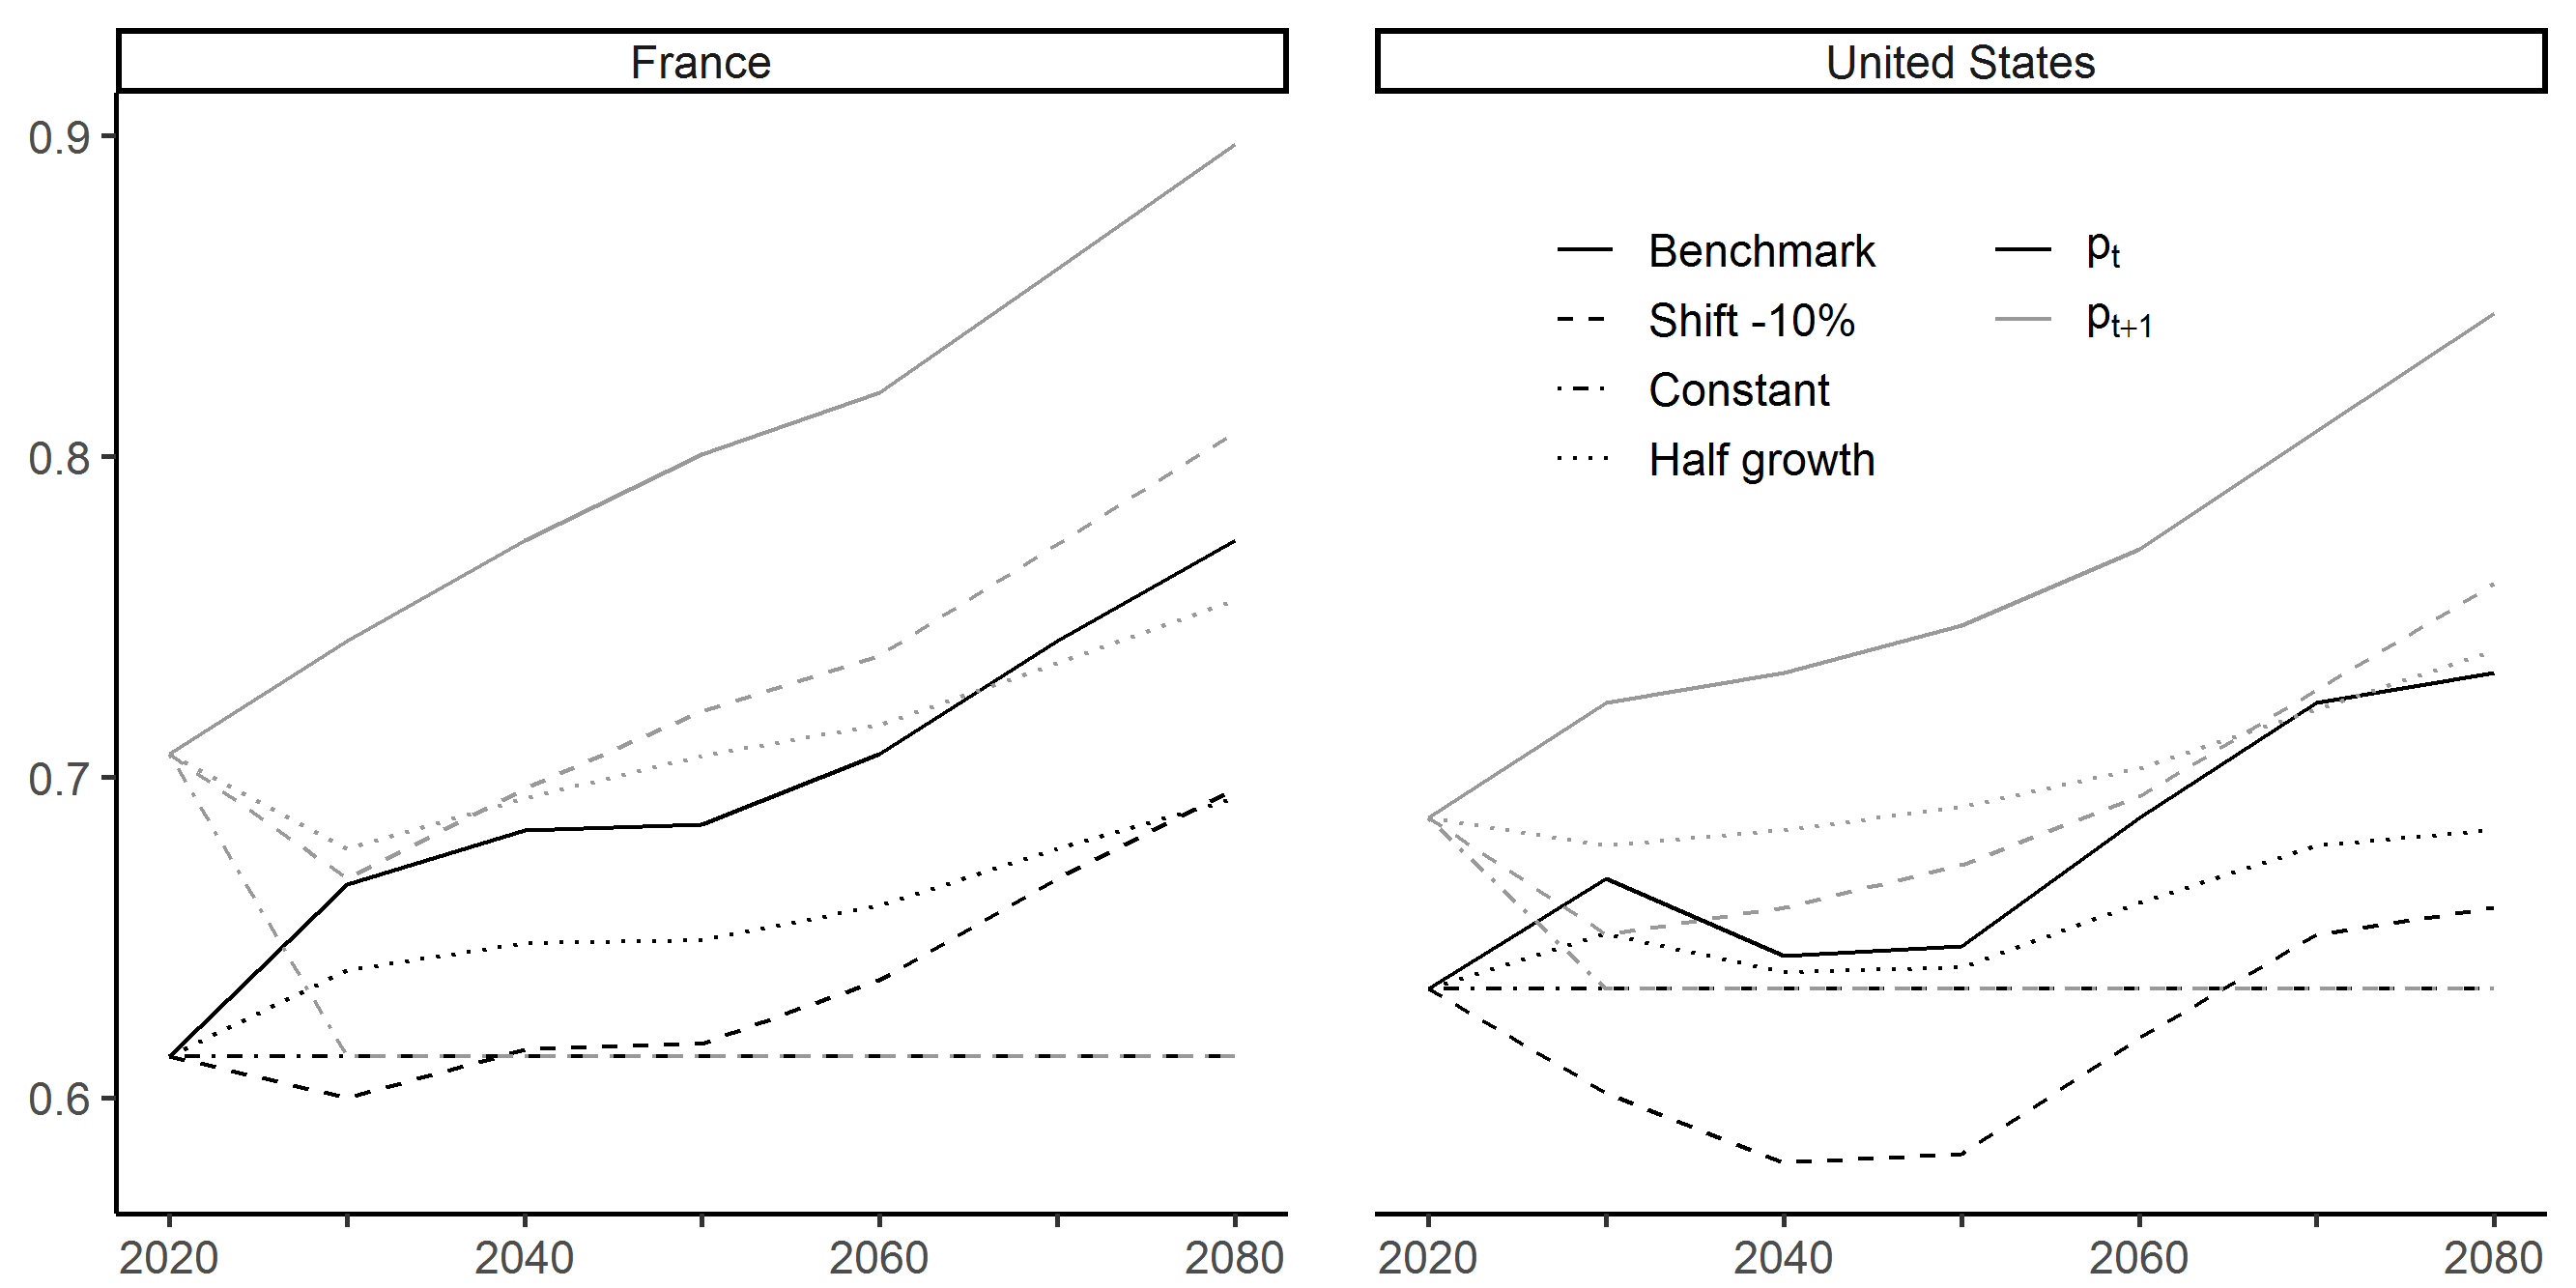
\includegraphics[width=1\linewidth]{../result/retirement/retage_p.png}
	\caption{Survival rate dynamics with changing retirement age specifications}
	\label{fig:retage_p}
	%		\vspace{.5ex}
	%		\hrule
	%		\vspace{-4ex}
	%		\justify\singlespacing\footnotesize 
\end{figure}
The red curves correspond to the first scenario that is mentioned above where the survival rate is shocked by -10\% in 2030 and keeps its growth rate thereafter. The blue and green curves are two special cases of the second scenario. The blue curves refers to the case where $\zeta = 0$, so the survival rate remains constant after 2030. It means that variations in retirement age are fully proportional to those in life expectancy. While the green curves coincide to the case where $\zeta = .5$. Thus, the survival rate $p_t$ grows at half of the speed of the benchmark simulation.

Figure \ref{fig:retage_ls} displays model predictions of the labor share according to the scenario.
\begin{figure}[tb]
	\centering
	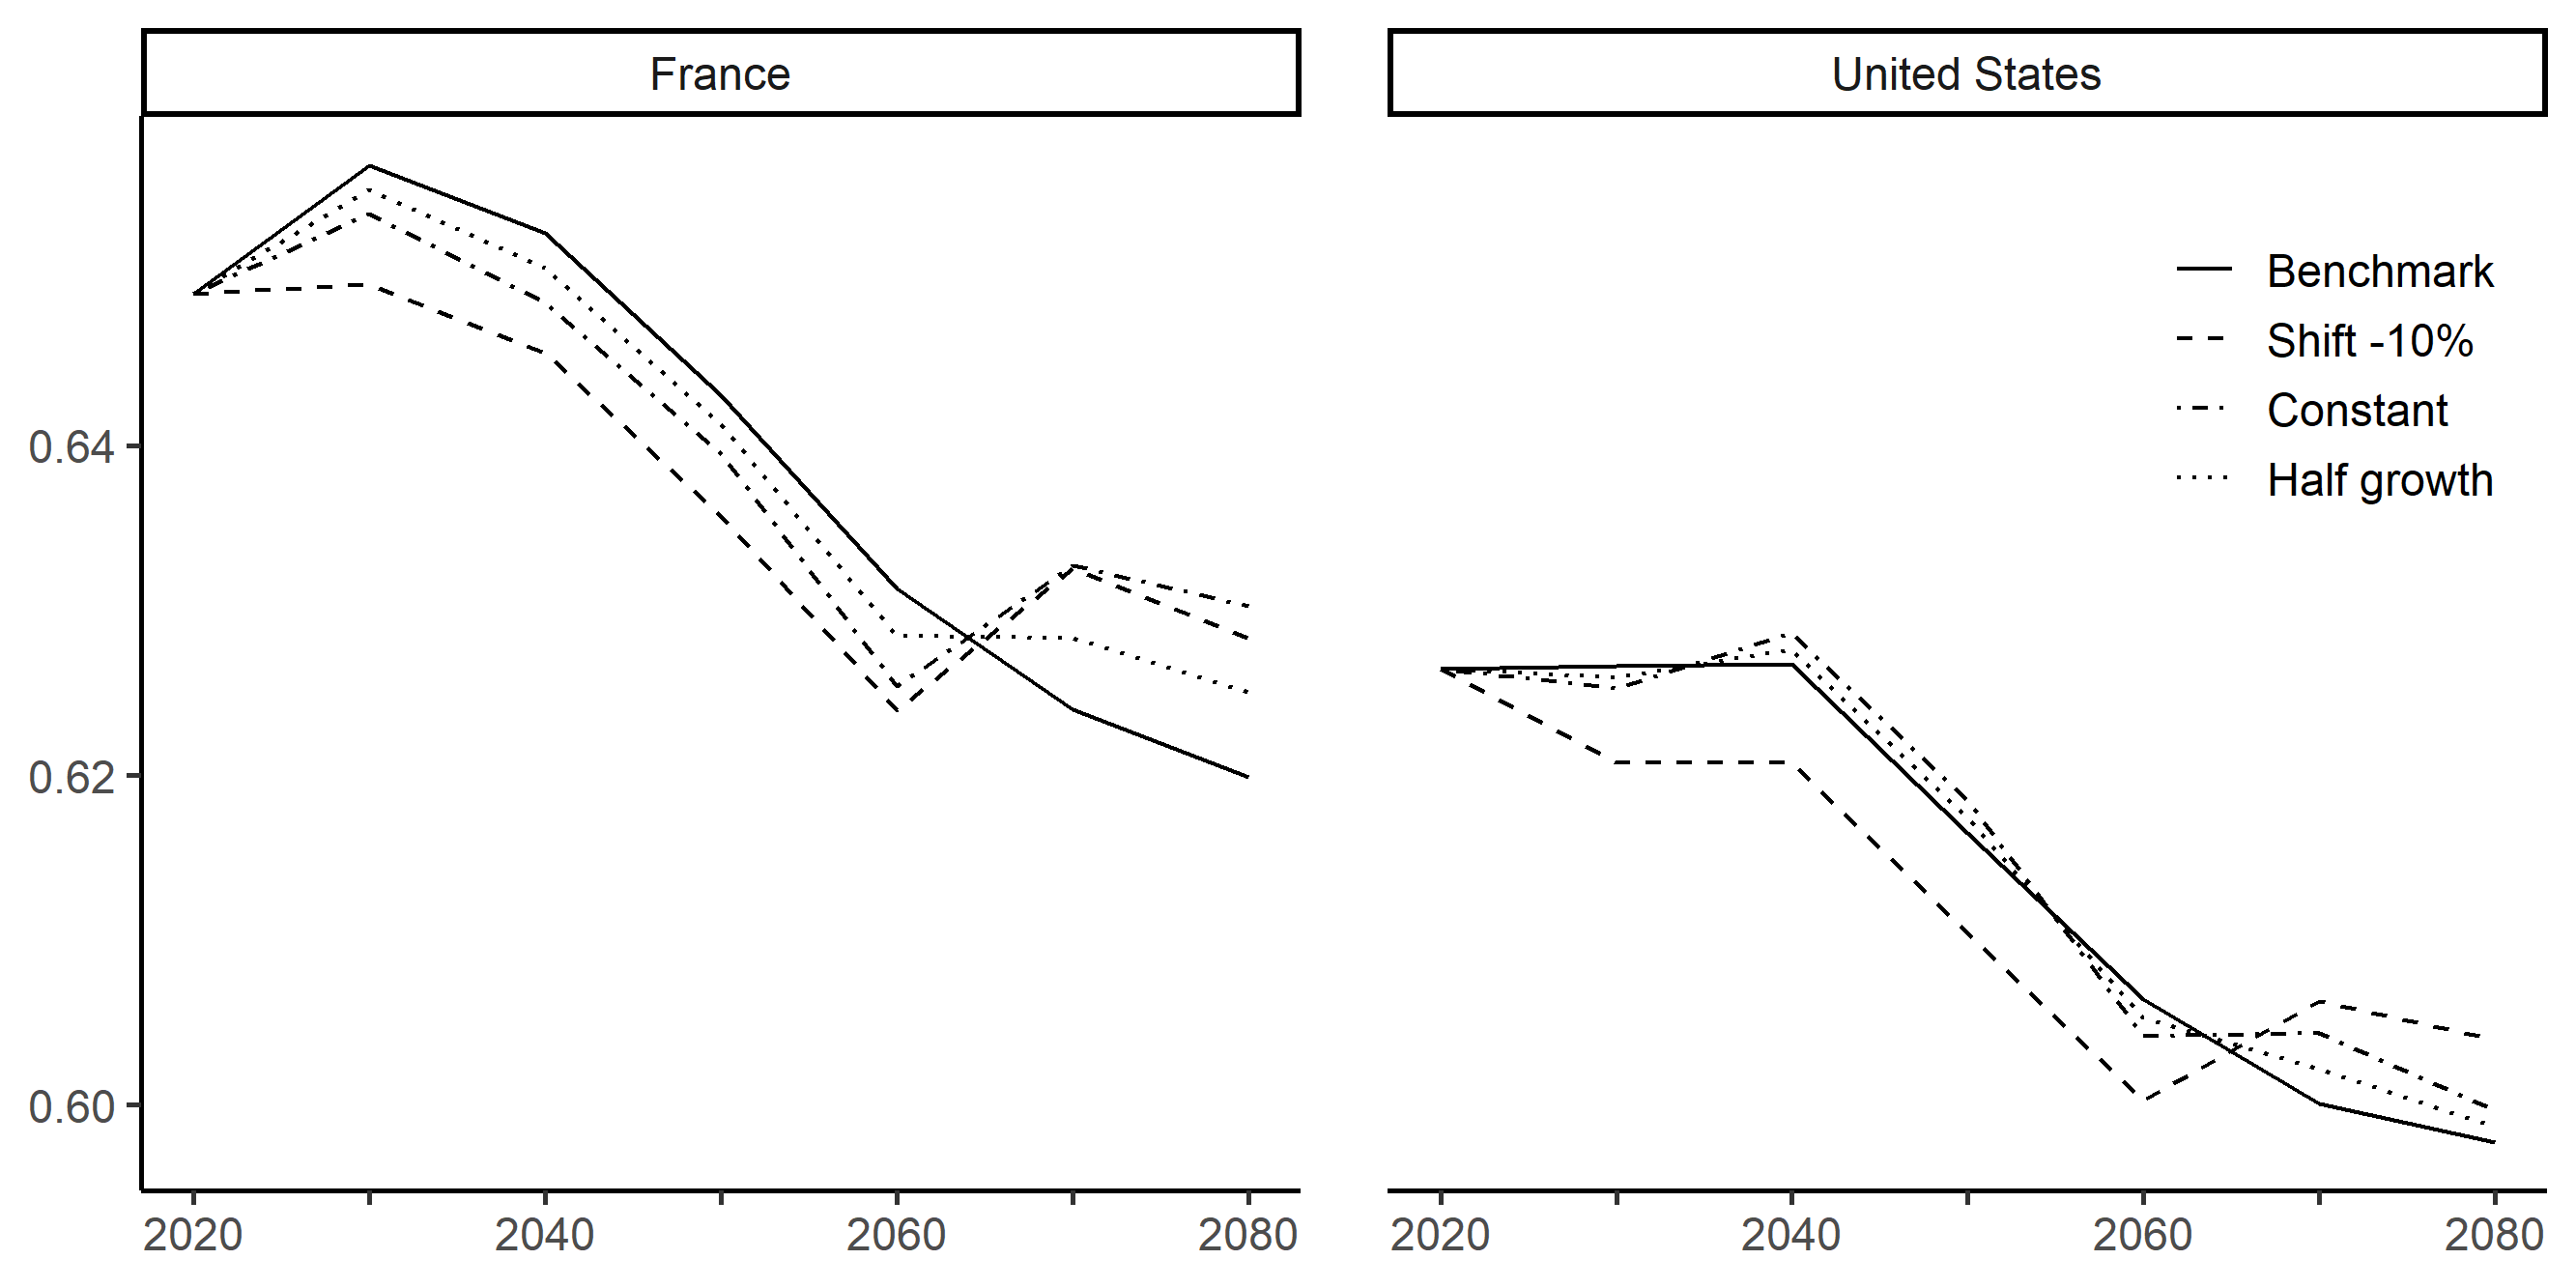
\includegraphics[width=1\linewidth]{../result/retirement/retage_ls.png}
	\caption{Model predictions of the labor share with changing retirement age specifications}
	\label{fig:retage_ls}
%		\vspace{.5ex}
%		\hrule
%		\vspace{-4ex}
%		\justify\singlespacing\footnotesize The solid black curve corresponds to the labor share from the benchmark prediction. Dashed curves correspond to different changes in retirement age. \textit{Shift -10\%} corresponds
\end{figure}
The raise of the age of retirement in France leads to a decline of the labor share with respect to the benchmark simulation in a first phase. In a second phase, the very long-run, the labor share is relatively greater than in the benchmark case. This result holds regardless of the scenario. In the United-States, the impact on the labor share depends on the scenario. As in France, the -10\% shift scenario generates a sharper decline of the labor share before to exceed the benchmark simulation's one in the very long-run. However, both scenarii of diminished growth of the survival rate have roughly the same pattern of the benchmark labor share. But there are still above the labor share in the very long-run. Therefore, changing the retirement age may have different impact on the labor share according to the country.

% Mechanisms
The underlying mechanisms are related to those detailed in section \ref{sec:quantitative_analysis}. However, there is a particularity to this change of the retirement age. The capital stock does not immediately adjust in the model. Because it has been determined by the savings of the previous period of each sequence, where the expected survival rate $p_{t+1}$ was much greater than the after-reform one $p^\prime_{t+1}$. This specificity cancels part of the direct cohort effect. This relatively high amount of available capital stock plays in favor of the firm within the wage bargaining. Because the firm is all the more able to substitute labor with capital. On the indirect cohort effect's side, the agents remain young longer due to the increase of the retirement age. This is translated in terms of the model with a decrease of the number of old households and an increase of the number of young households. Thus, the youth has more political weight than in the benchmark case. With this political strength, they raise their outside option through pro-young public policies which allows them to bargain greater wages. As a response, the firm shift away from labor and hire relatively less workers than in the benchmark case. As mentioned above, the relatively high amount of available capital stock due to the \textit{stickiness} enables the firm to substitute all the more.


	
	\section{Conclusion} \label{sec:conclusion}
	The literature on the labor share has emphasized the role of many factors such as the biased technical change or the labor market institutions. I built an OLG model in which labor market institutions are endogenously determined through public policy and affect the wage bargaining. Using this model, I analyze the impact of demographic dynamics on labor share's long-term dynamics in France and the United-States. The simulation is able to replicate data for both countries since the 1970s.
% I use the argument developed by \cite{Caballero1998} where firms shifted away from labor as a response of worker's ability to obtain a relatively high labor share. Workers and unions are able to do so due to labor market institutions.

%% Mechanisms

%I highlight the different determinants and channels through which demographic dynamics affect the labor share.
%The model is able to replicate data for France and the United-States. 
Model predictions suggest that the decline of the labor share during the last decades was driven by cohort-size effects. 
For France, the baby-boomers cohort seems to drive the public policy and thus the way in which national income is allocated between labor and capital.
When the baby-boomers cohort enters on the labor market, they shape the labor market institutions in their favor because they face an unemployment risk. Opportunistic political candidates implements public policy desired by this cohort. 
Thus, these more protective labor market institutions rise workers' outside option which enables unions to bargain greater wages. 
As a response, firms shift away from labor and use more capital. This mechanism is due to the fact that both input factors are gross substitute and that the firms have the prerogative to hire and fire.
The unemployment rate rises and so does the production-per-worker. 
The increase of the production-per-worker offsets the one of the wage rate. 
Therefore, the labor share declines over the end of the twentieth century. 
Thereafter, the baby-boomers retire and trigger the opposite mechanism. 
Although the public policy shrinks the outside option of workers within the wage bargaining which should reduce wages and raise employment. 
The capital stock has sharply increased due to massive savings of the baby-boomers when they were young. 
The important available capital stock partially thwart the reverse mechanism and the labor share does not recover its past level.
The model predicts a slight resurgence of the labor share for the next decades in France and a stagnation in the United-States.

%% Results

Model predictions suggest that the survival rate dynamics have a larger impact on the labor share than the population growth dynamics. I also decompose this impact between two channels: the direct cohort-size effect and the indirect cohort-size effect. The former dominates for France when the baby boomers are young, while the latter takes the lead once this cohort retires. Although the labor share declined due to public policies implemented by baby boomers, their after-tax income did not. Because they also increased the redistribution through taxes. An increase of the retirement age should decrease the labor share in the following decades due to the over-accumulation of capital and the raising political power of the youth. However, the labor share is expected to be greater in the very long-run.

%% Main assumptions
The two main hypothesis of the paper are about the elasticity of substitution between capital and labor and the right-to-manage specification for the wage bargaining. Recent estimates suggest that this elasticity may be greater than one (see \citealt{Karabarbounis2014}) but an other part of the literature has found it below one, particularly for the United-States (see, for example, \citealt{Antras2004}; \citealt{Chirinko2008}). Moreover, I do not include any form of biased technical change within the model. This is voluntary in order to develop an other theory on the labor share's decline based on demographic dynamics. It could be the case that biased technical change is also driven by demographic dynamics through the \textit{grability} of workers to seize part of the rent. This grability may be generated by some cohorts which are sufficiently numerous to shape labor market institutions in their favor and therefore in favor of labor. I let the investigation of a potential endogenous biased technical change induced by demographic dynamics for further research.






	
	\clearpage
	\setlength\bibsep{0pt}
	\bibliographystyle{apalike}
	\bibliography{my_collec}
	
	\clearpage
	\onehalfspacing
	\appendix
	
	\section*{Appendix A. Uniqueness of the equilibrium} \label{appendix:uniqueness}
	\addcontentsline{toc}{section}{Appendix A. Uniqueness of the equilibrium}
	Let define, respectively, equations \eqref{eq:Xg} and \eqref{eq:Xh} with the functions $g(k_t, N_t^y, K_t, \eta_t; \phi, \sigma)$ and $h(k_t ; \gamma, \phi, \sigma)$ such as:
\begin{align*}
	g(k_t, N_t^y, K_t, \eta_t; \phi, \sigma) &= \ln\left( \frac{ \frac{N_t^y}{K_t} k_t - 1 } { \frac{\phi}{1-\phi} k_t^{\frac{\sigma-1}{\sigma}} \eta_t - 1 }\right) \\
	h(k_t ; \gamma, \phi, \sigma) &= \left( \sigma + \frac{1-\phi}{\phi} \frac{1-\gamma(1-\sigma)}{\gamma} k_t^{\frac{1-\sigma}{\sigma}} \right)^{-1}
\end{align*}

% \subsection*{A.1 Analysis of the $g$ function}

Due to the logarithm, we have two vertical asymptotes depending on whether the numerator or the denominator within the logarithm is equal to zero. The first vertical asymptote is the one associated to the numerator $k_1 = \frac{K_t}{N_t^y}$ and the second vertical asymptote is associated to the denominator $k_2 = \left(\frac{1-\phi}{\phi} \frac{1}{\eta_t}\right)^{\frac{\sigma}{\sigma-1}}$. Rewriting the $g$ function with these vertical asymptotes, I have:
\begin{equation*}
g(k_t, k_1, k_2; \sigma) = \ln\left( \frac{\frac{k_t}{k_1}-1}{\left(\frac{k_t}{k_2}\right)^{\frac{\sigma - 1}{\sigma}} - 1} \right)
\end{equation*}
This function has four different shapes according to the value of $\sigma$ and both vertical asymptotes ($k_1$ and $k_2$). Figure \ref{fig:g_shape} plots these shapes.
\begin{figure}[tb]
	\begin{subfigure}[b]{0.5\linewidth}
		\centering
		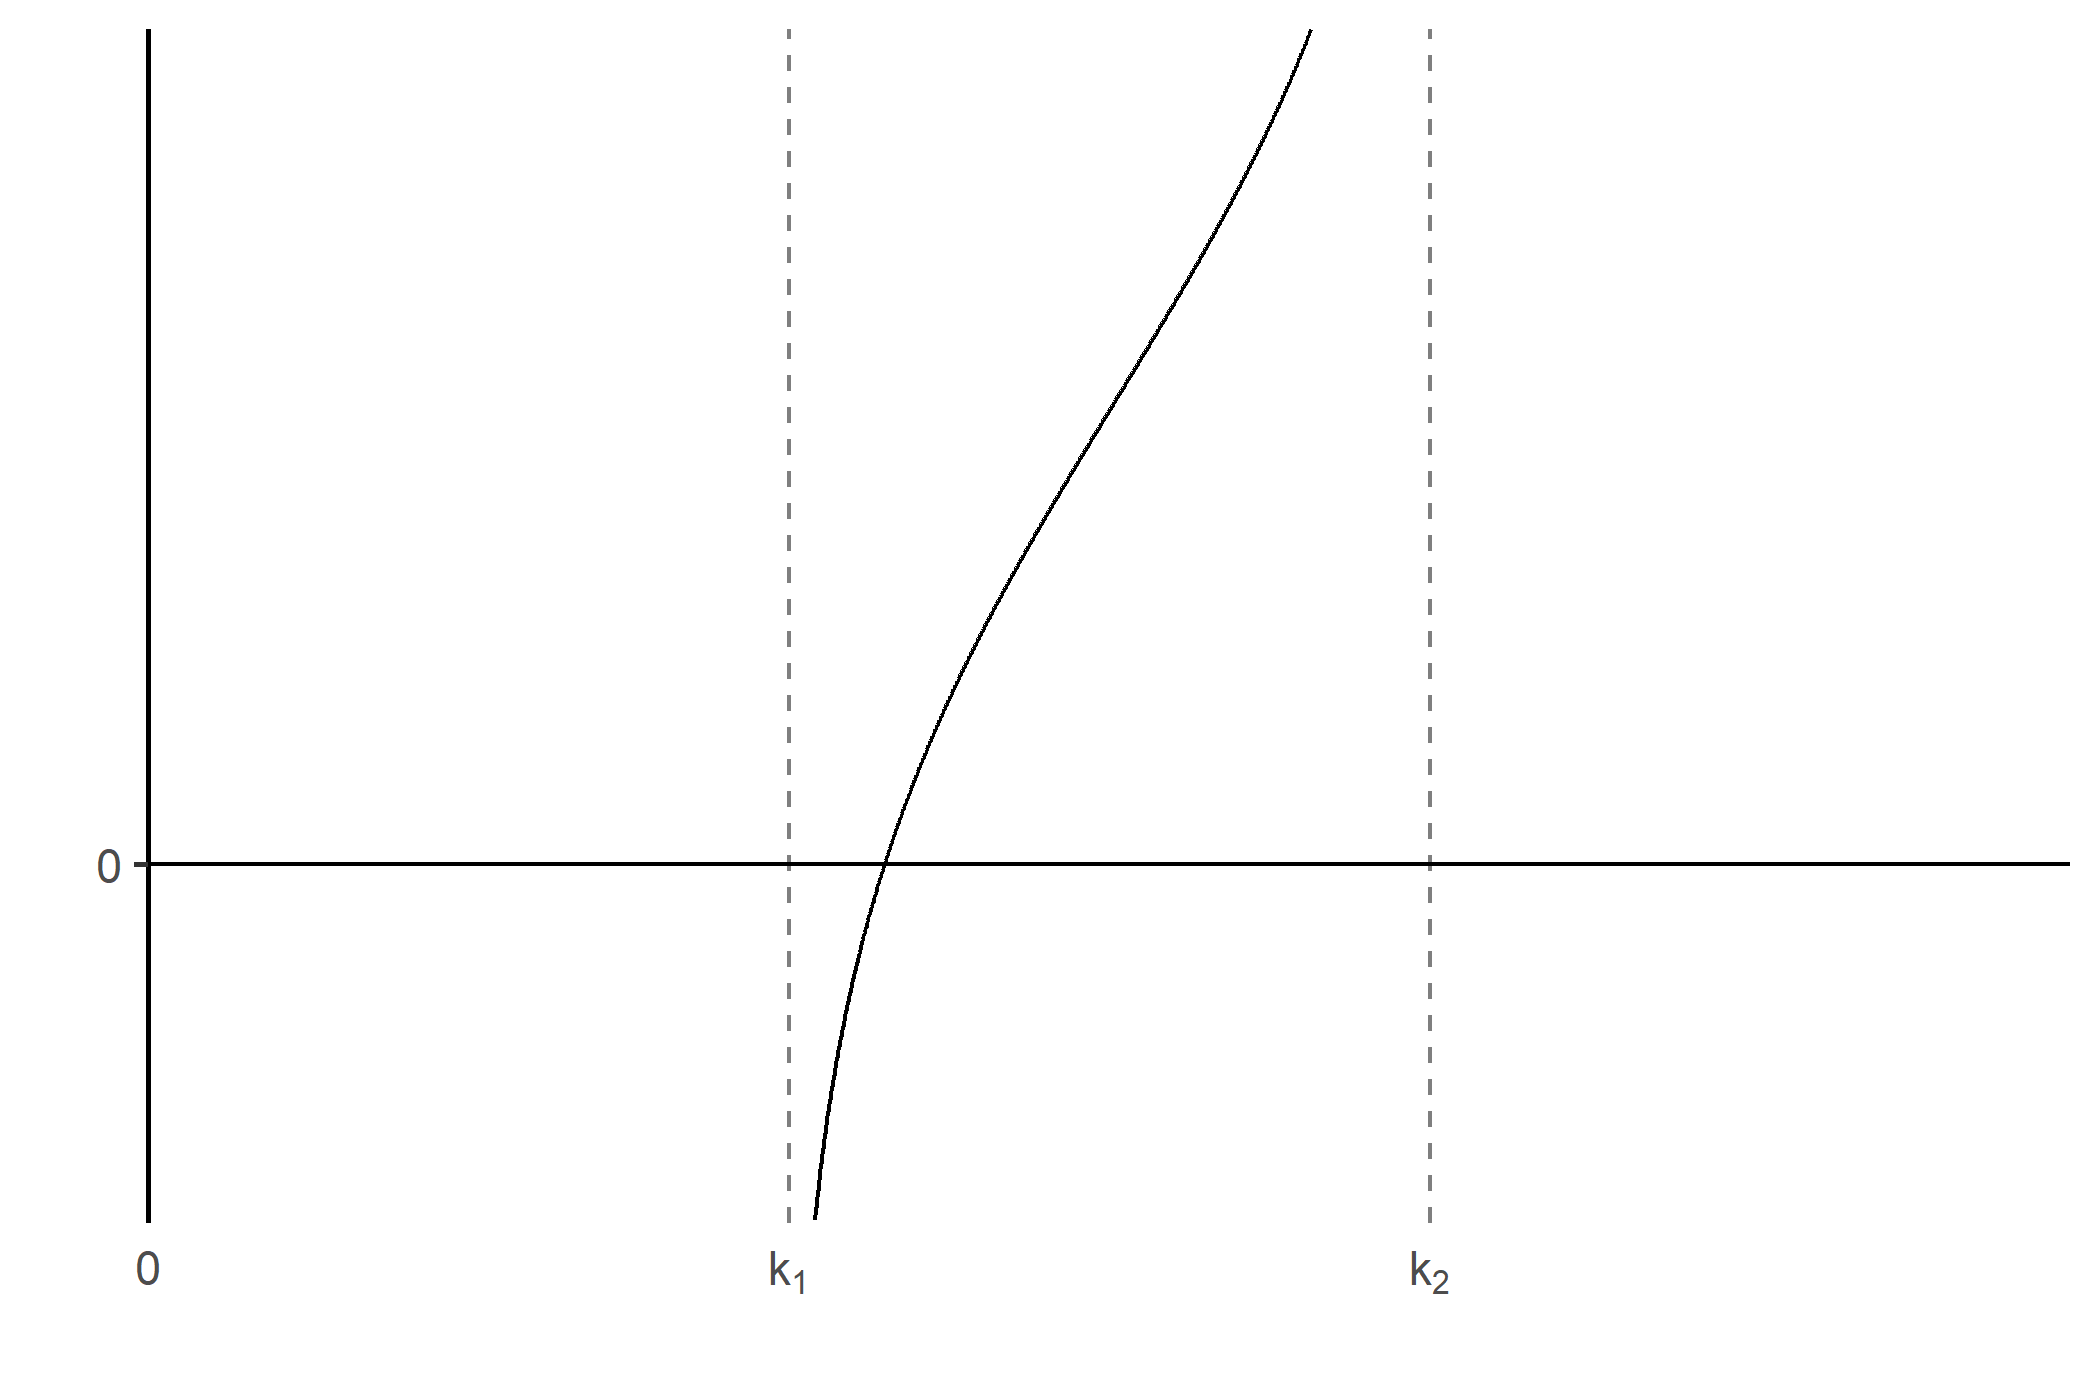
\includegraphics[width=1\linewidth]{../result/appendix_A/function_g/graph_a.png} 
		\caption{$\sigma < 1$, $k_1 < k_2$} 
		\label{fig:g_shape_a}
	\end{subfigure}
	\begin{subfigure}[b]{0.5\linewidth}
		\centering
		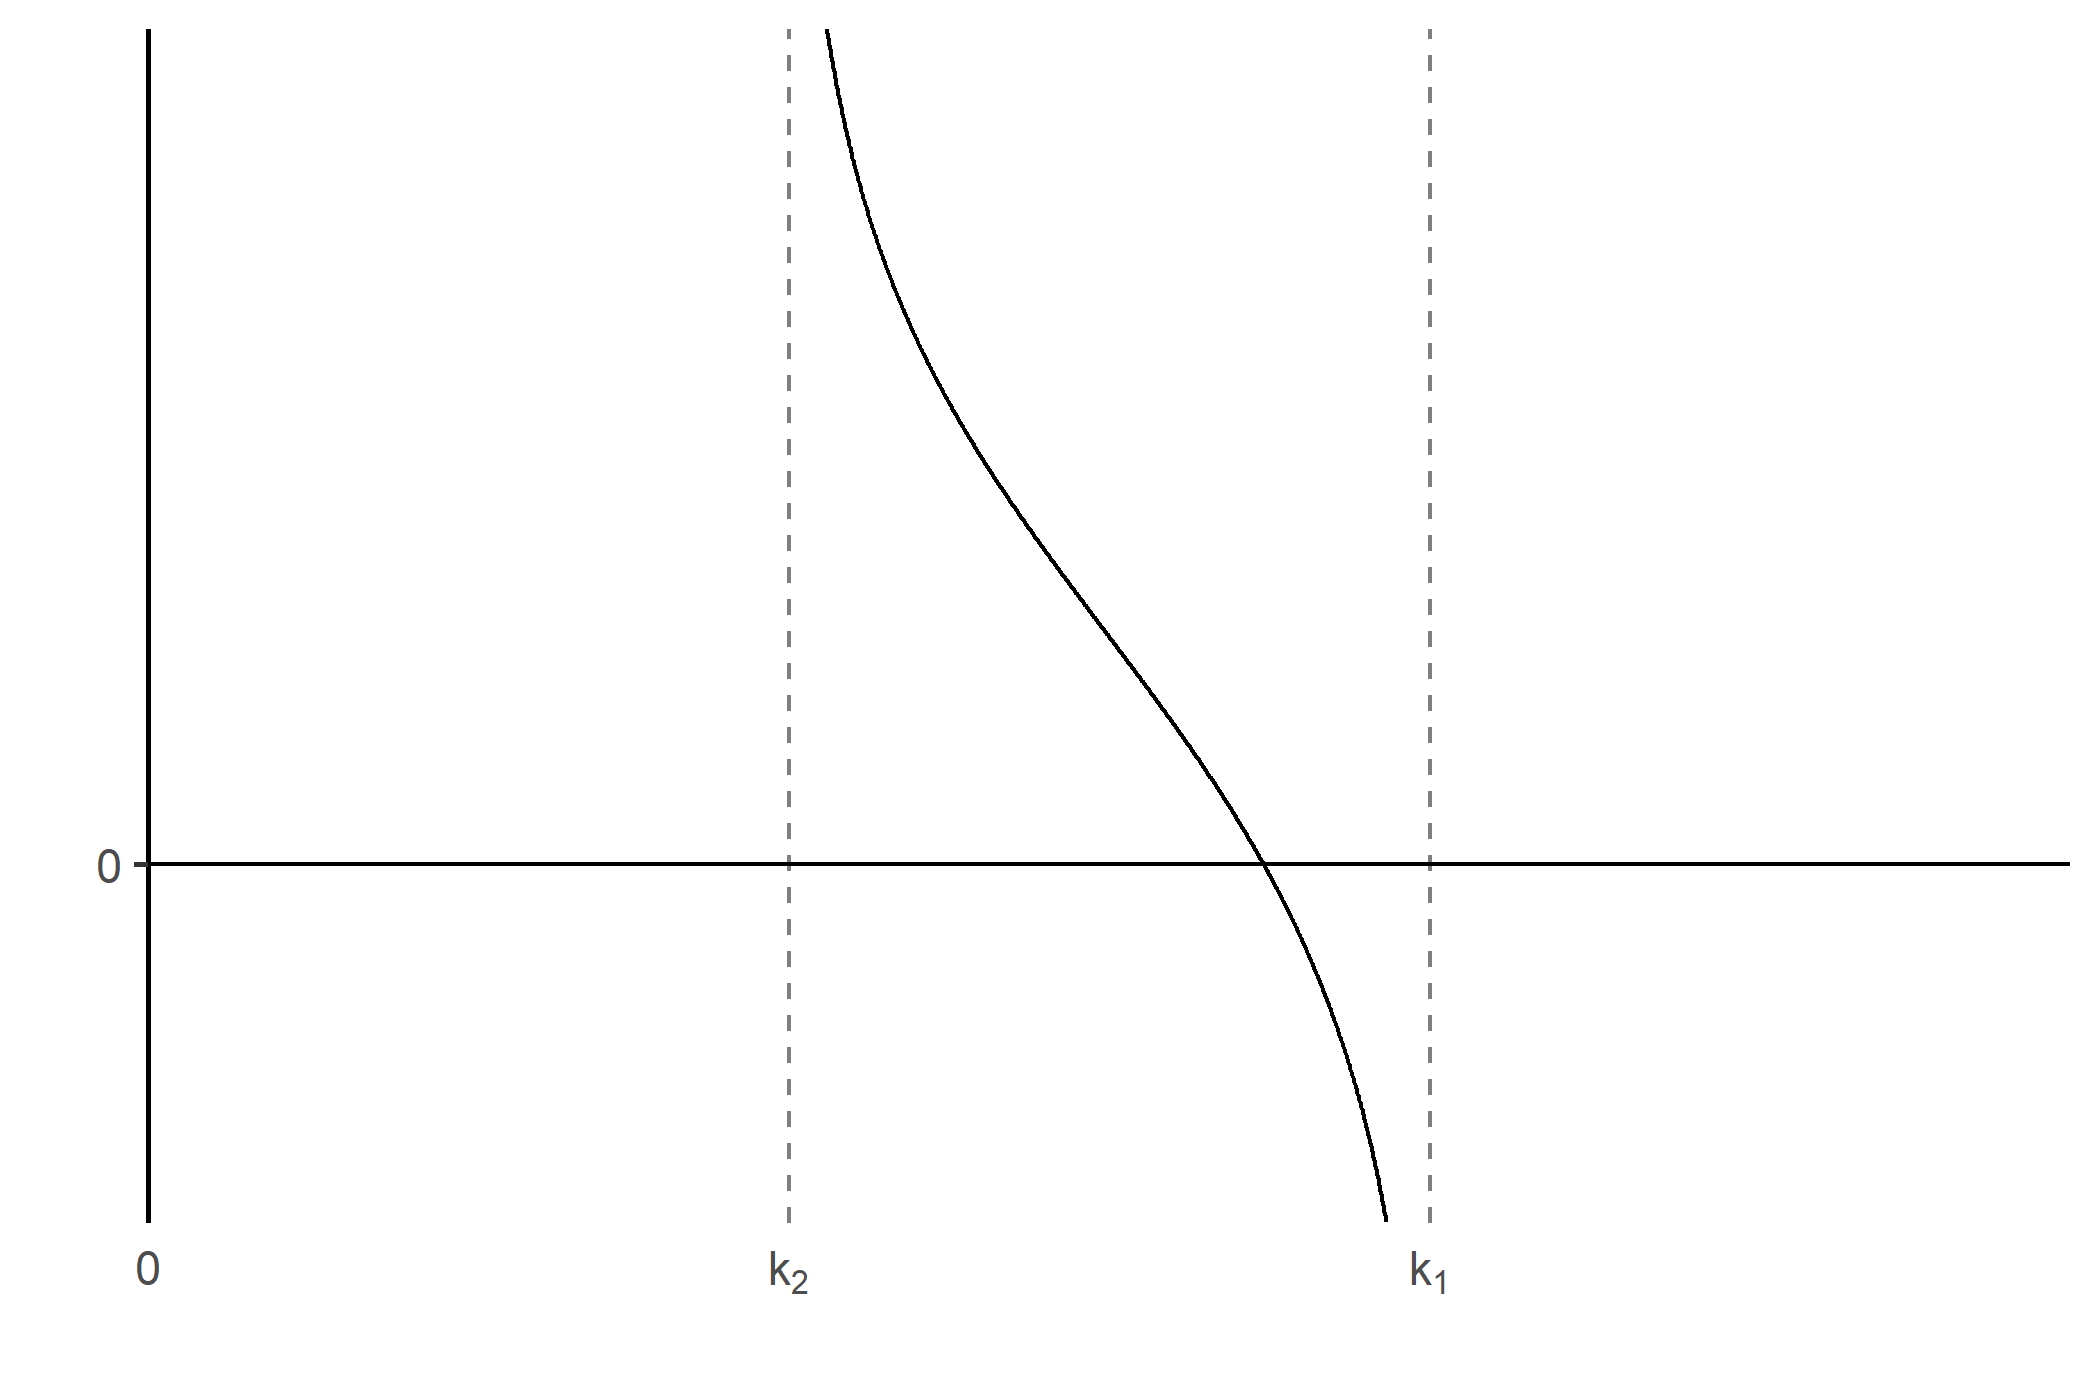
\includegraphics[width=1\linewidth]{../result/appendix_A/function_g/graph_b.png} 
		\caption{$ \sigma < 1$, $k_1 > k_2$}
		\label{fig:g_shape_b}
	\end{subfigure}
	%%%
	\begin{subfigure}[b]{0.5\linewidth}
		\centering
		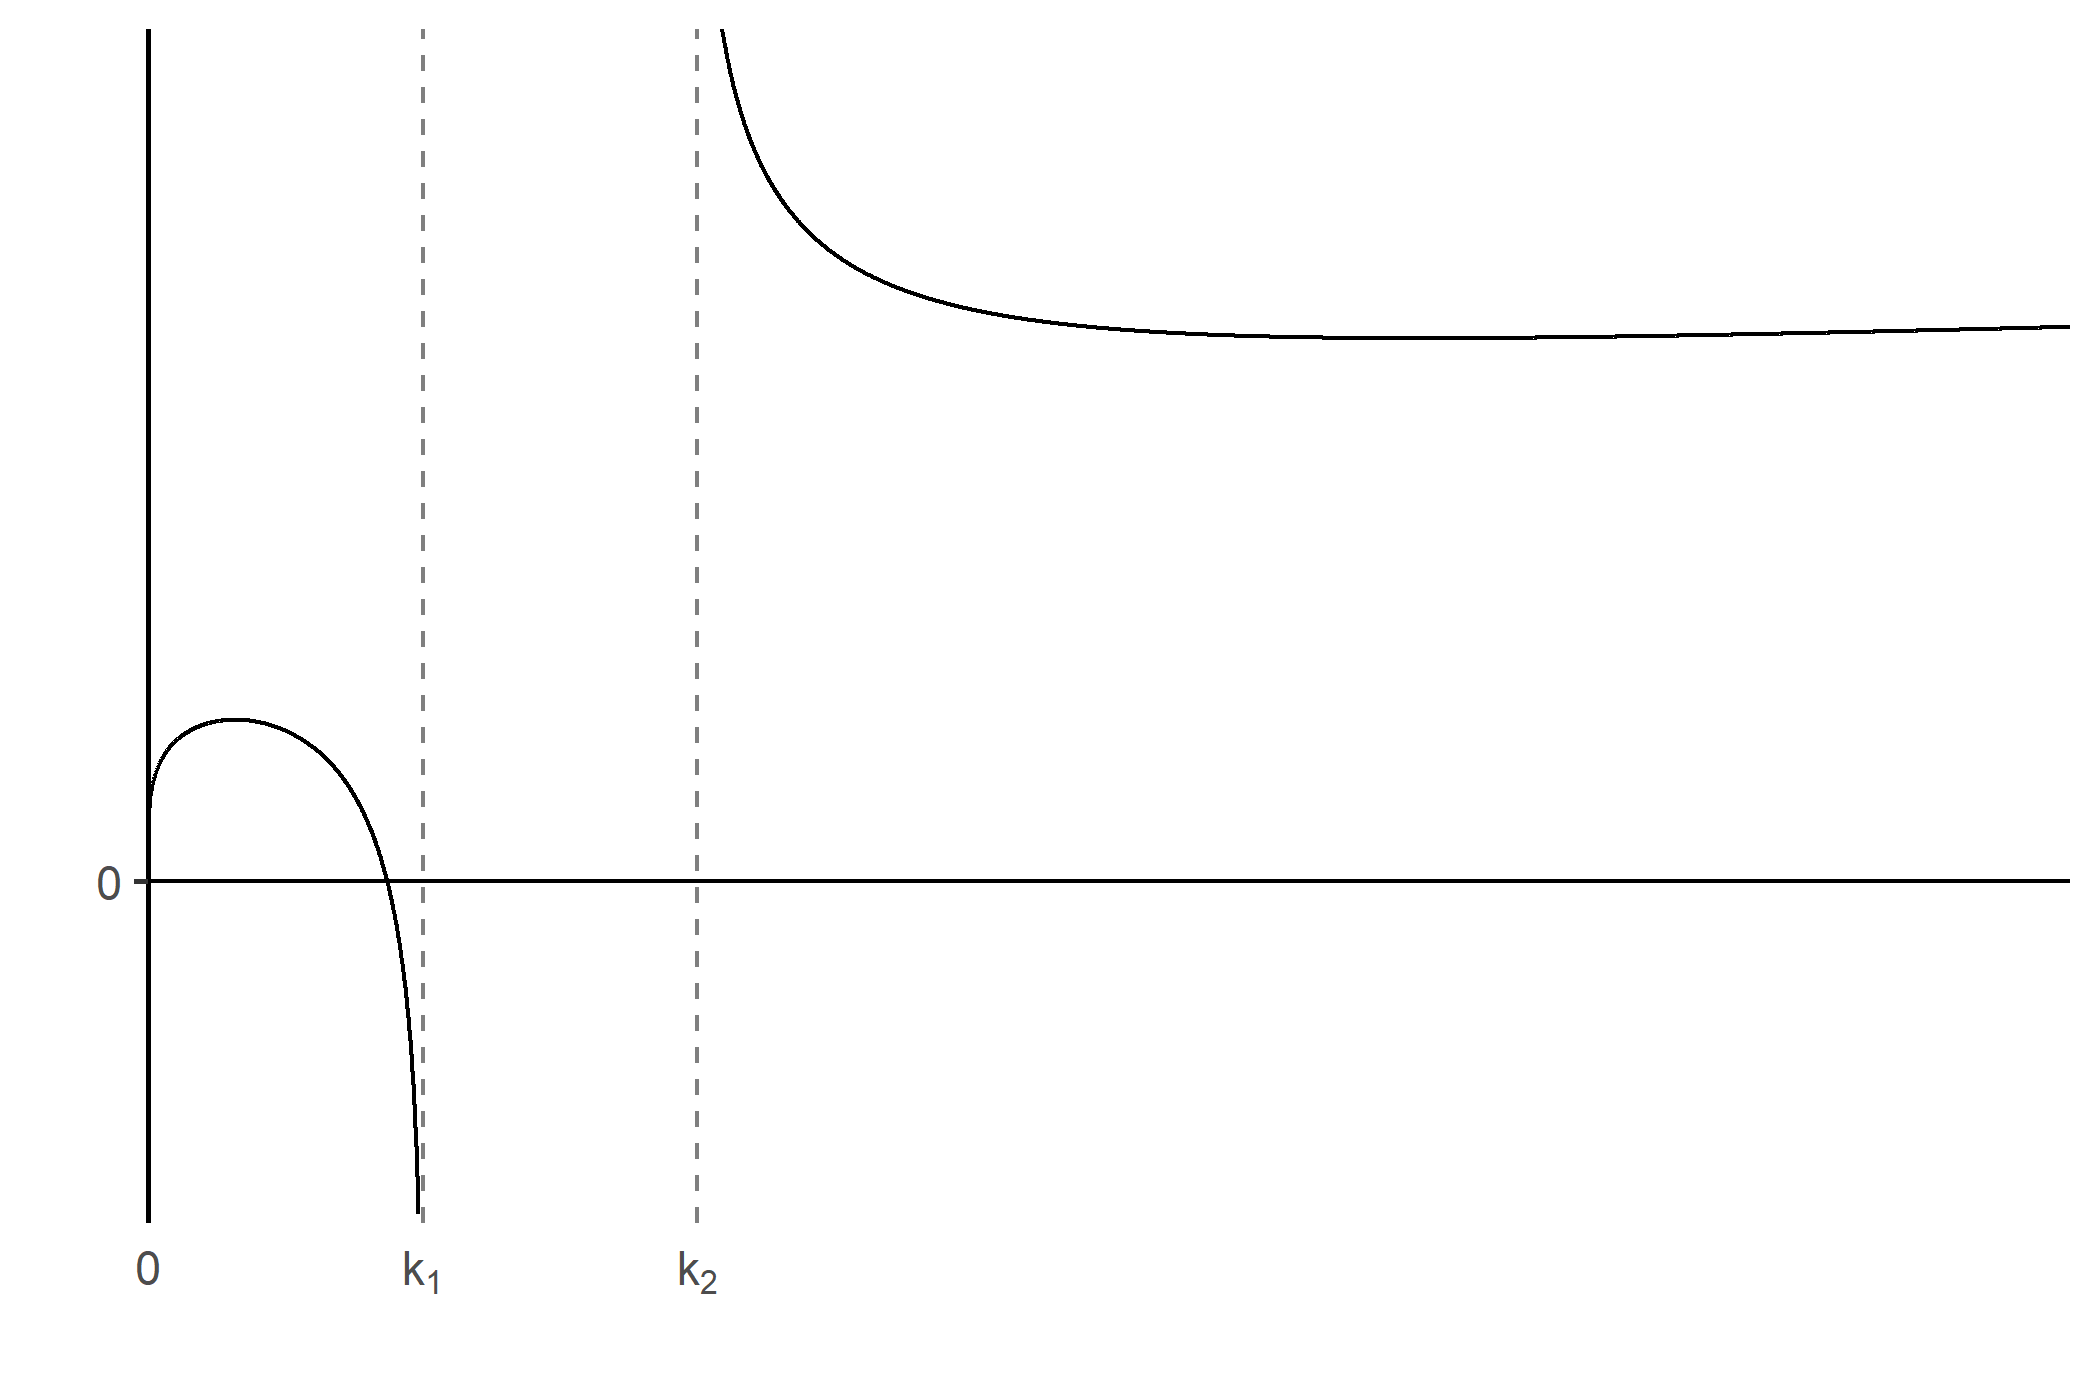
\includegraphics[width=1\linewidth]{../result/appendix_A/function_g/graph_c.png} 
		\caption{$\sigma > 1$, $k_1 < k_2$}
		\label{fig:g_shape_c}
	\end{subfigure}
	\begin{subfigure}[b]{0.5\linewidth}
		\centering
		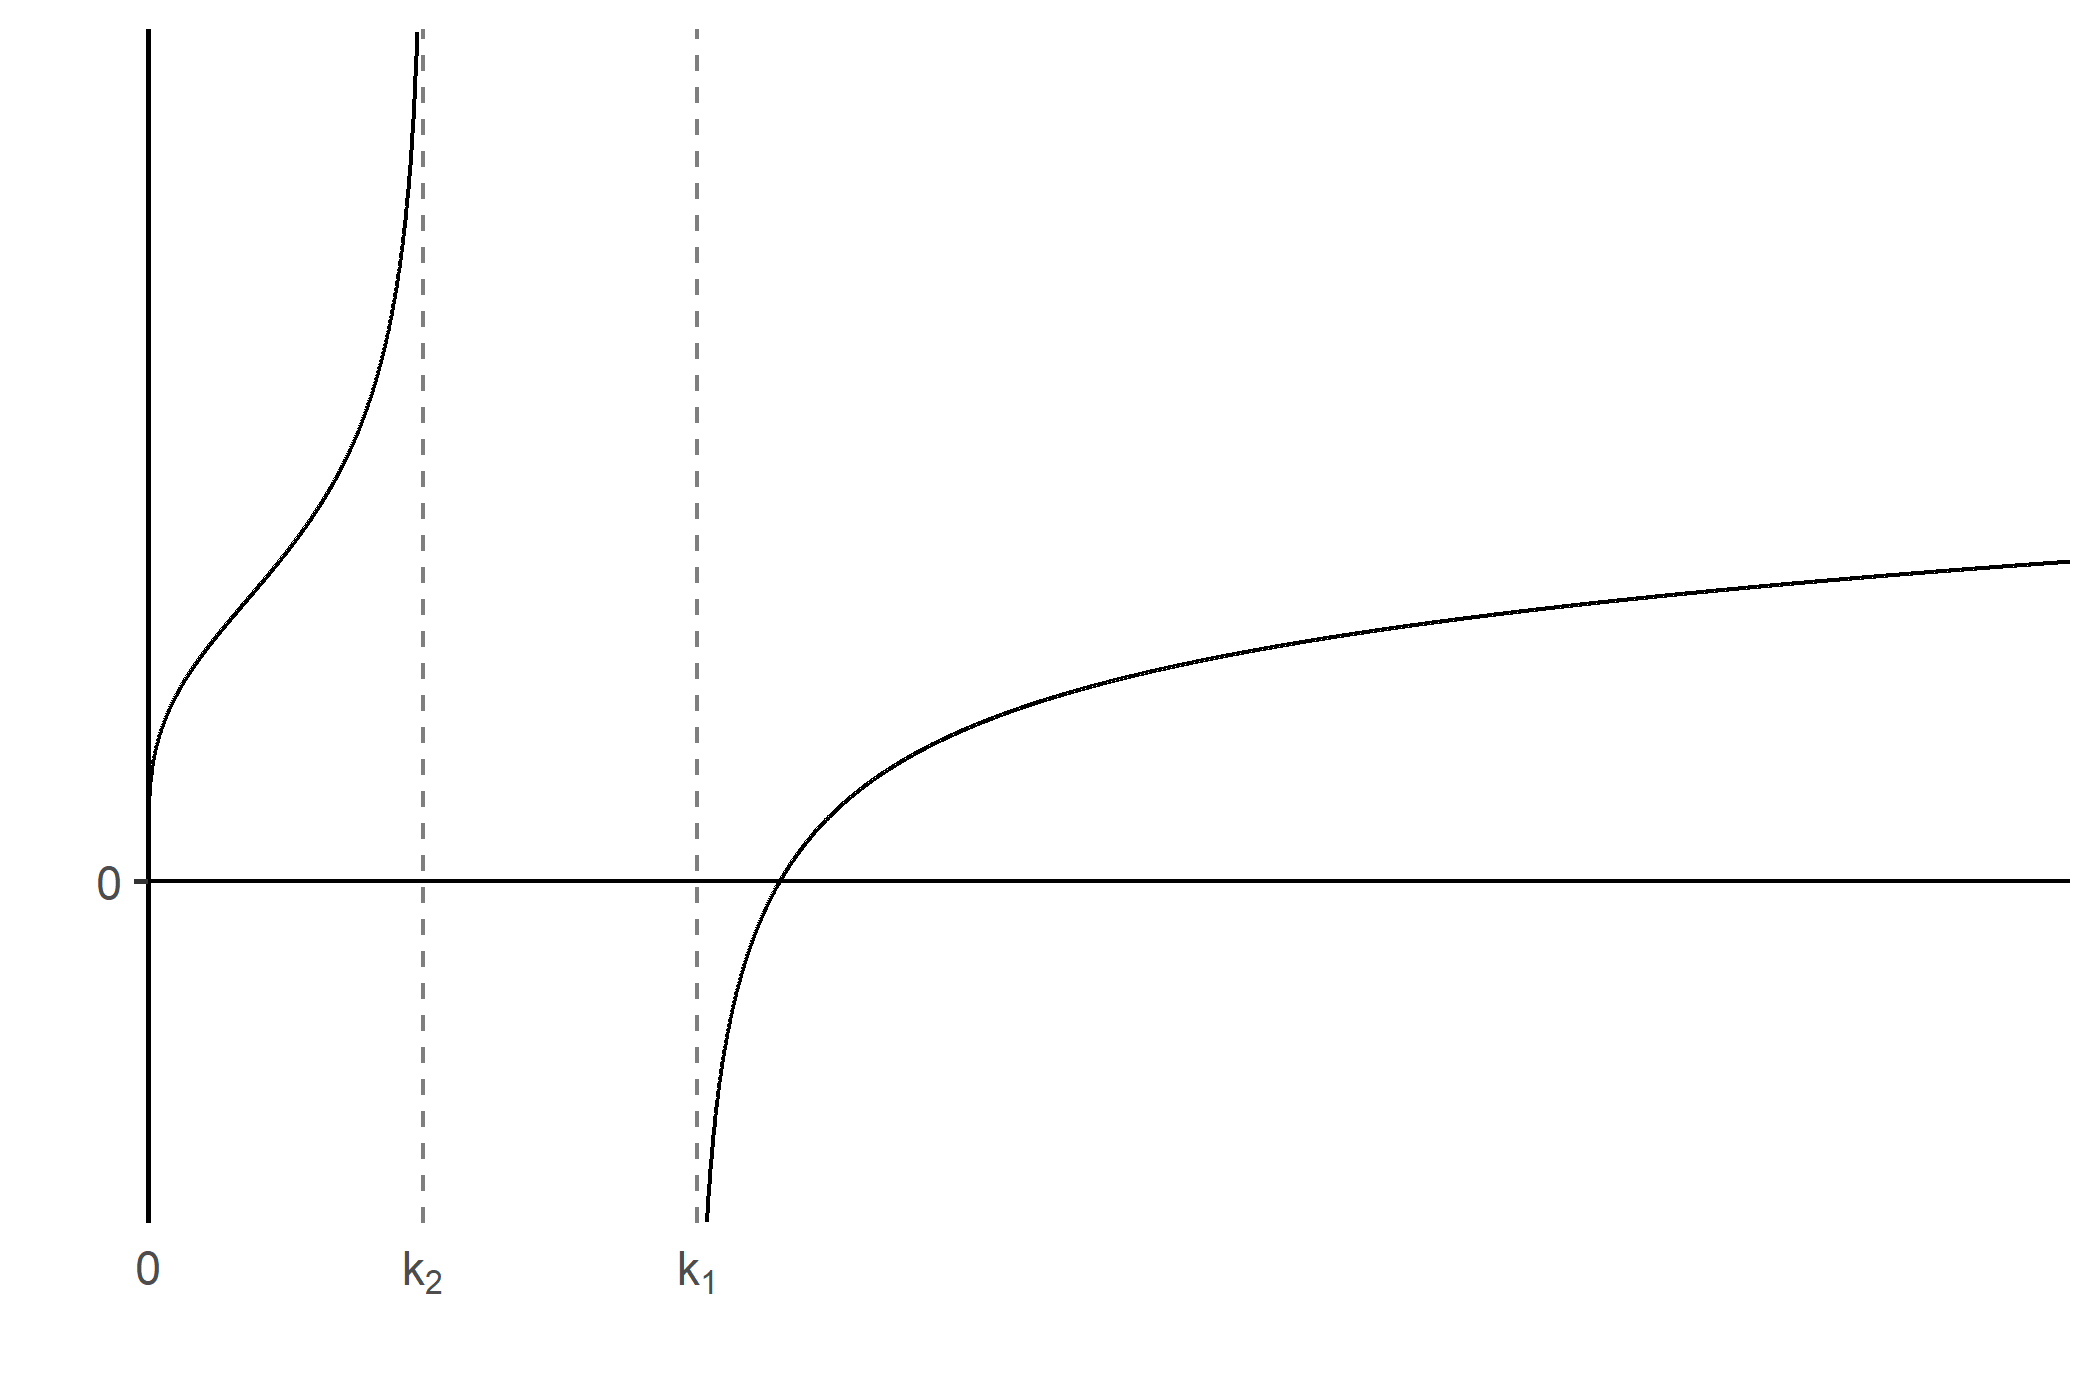
\includegraphics[width=1\linewidth]{../result/appendix_A/function_g/graph_d.png}
		\caption{$\sigma > 1$, $k_1 > k_2$}
		\label{fig:g_shape_d}
	\end{subfigure} 
	\caption{Different possible shapes of the $g$ function, according to the value of $\sigma, k_1, k_2$.}
	\label{fig:g_shape}
	\vspace{.5ex}
	\hrule
	\vspace{-4ex}
	\justify\singlespacing\footnotesize The x-axis corresponds to $k_t$. The function graphs are drawn using numerical computation with the following set of parameters for each case:\\
	(a) $\sigma = 0.8$, $k_1 = 1$, $k_2 = 2$ ; \hspace{2ex}(b) $\sigma = 0.8$, $k_1 = 2$, $k_2 = 1$ ; \\(c) $\sigma = 1.2$, $k_1 = 1$, $k_2 = 2$ ; \hspace{2ex}(d) $\sigma = 1.2$, $k_1 = 2$, $k_2 = 1$.
\end{figure}
The $h$ function has three different shapes according to the value of $\sigma$. Figure \ref{fig:h_shape} plots these shapes.
\begin{figure}[tb]
	\begin{subfigure}[t]{0.32\linewidth}
		\centering
		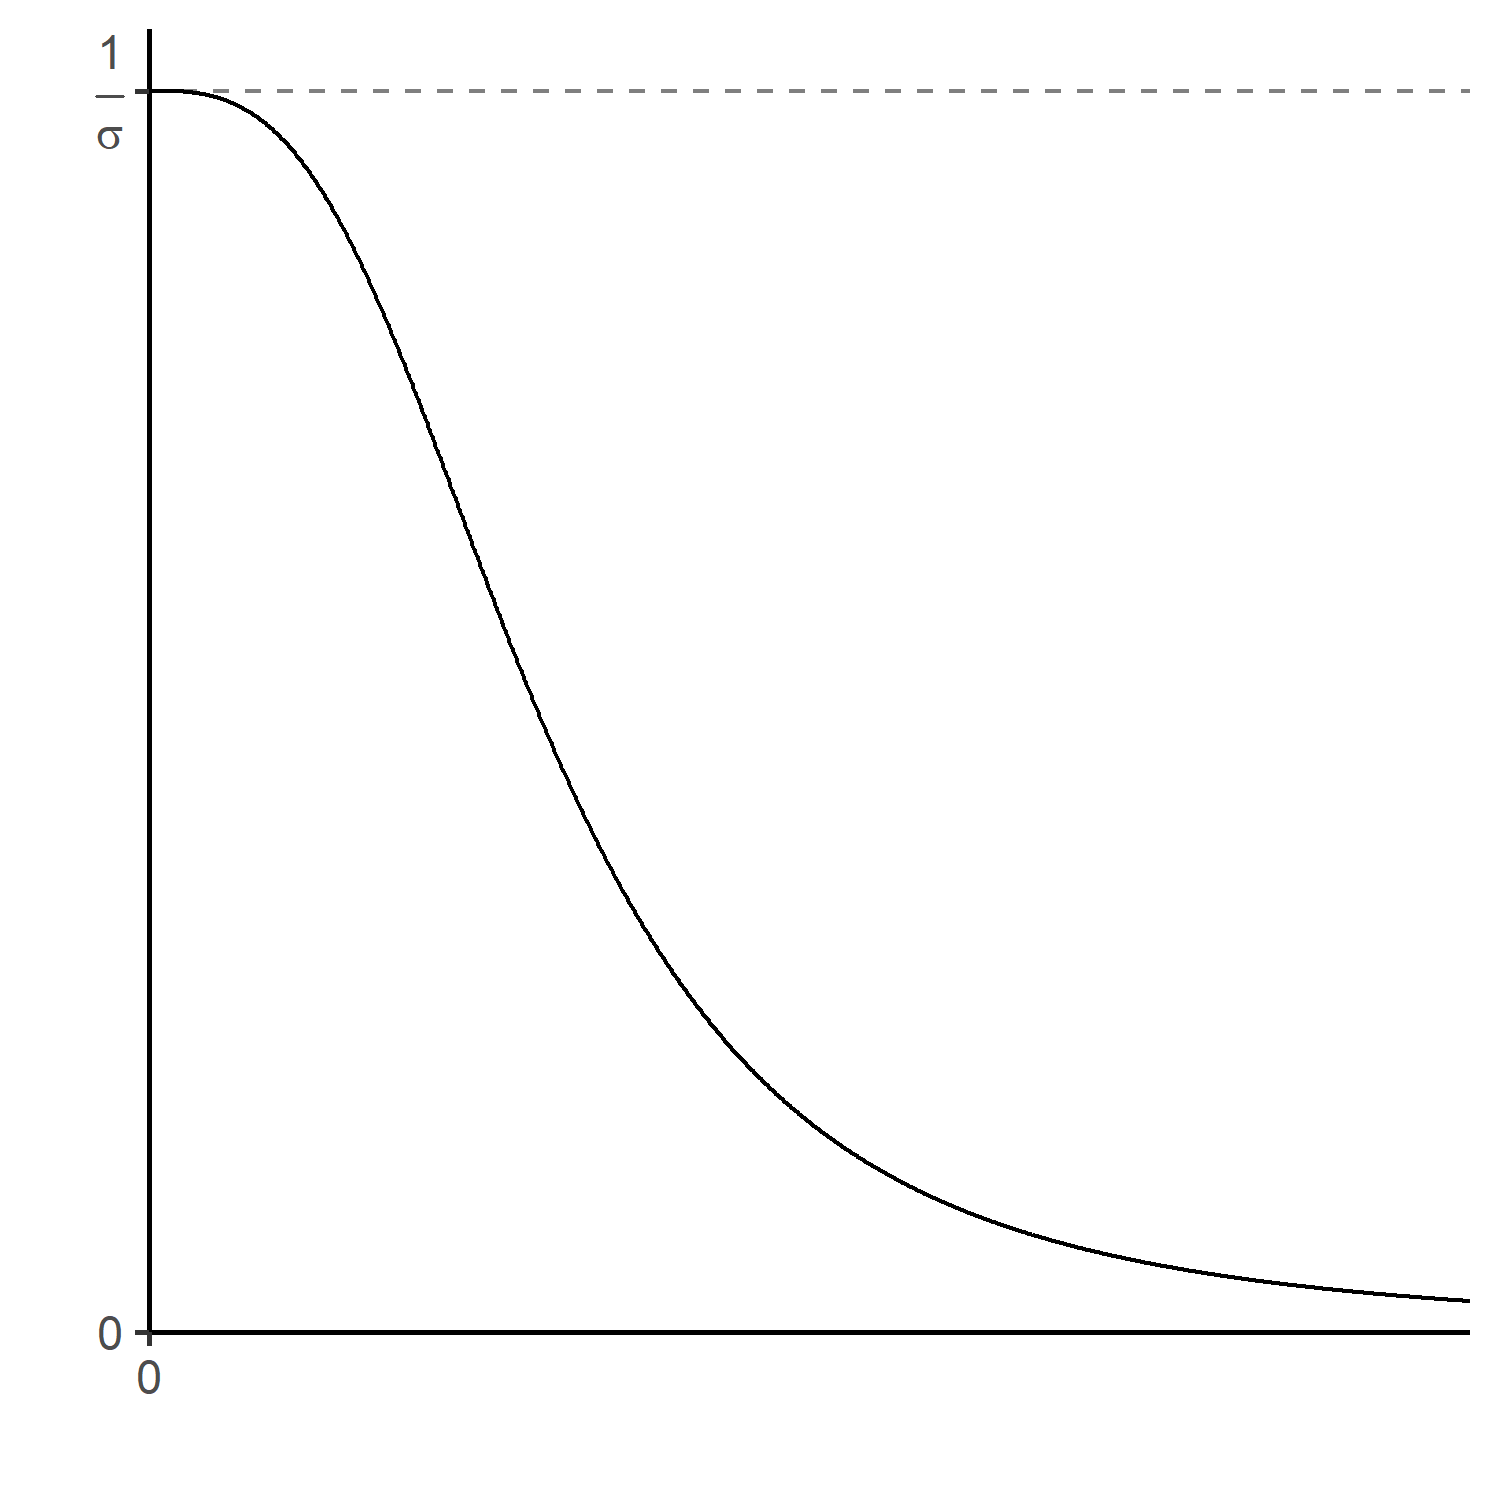
\includegraphics[width=1\linewidth]{../result/appendix_A/function_h/graph_1.png} 
		\caption{$\sigma \leq 0.5$} 
		\label{fig:h_shape_1} 
	\end{subfigure}
	%%%
	\begin{subfigure}[t]{0.32\linewidth}
		\centering
		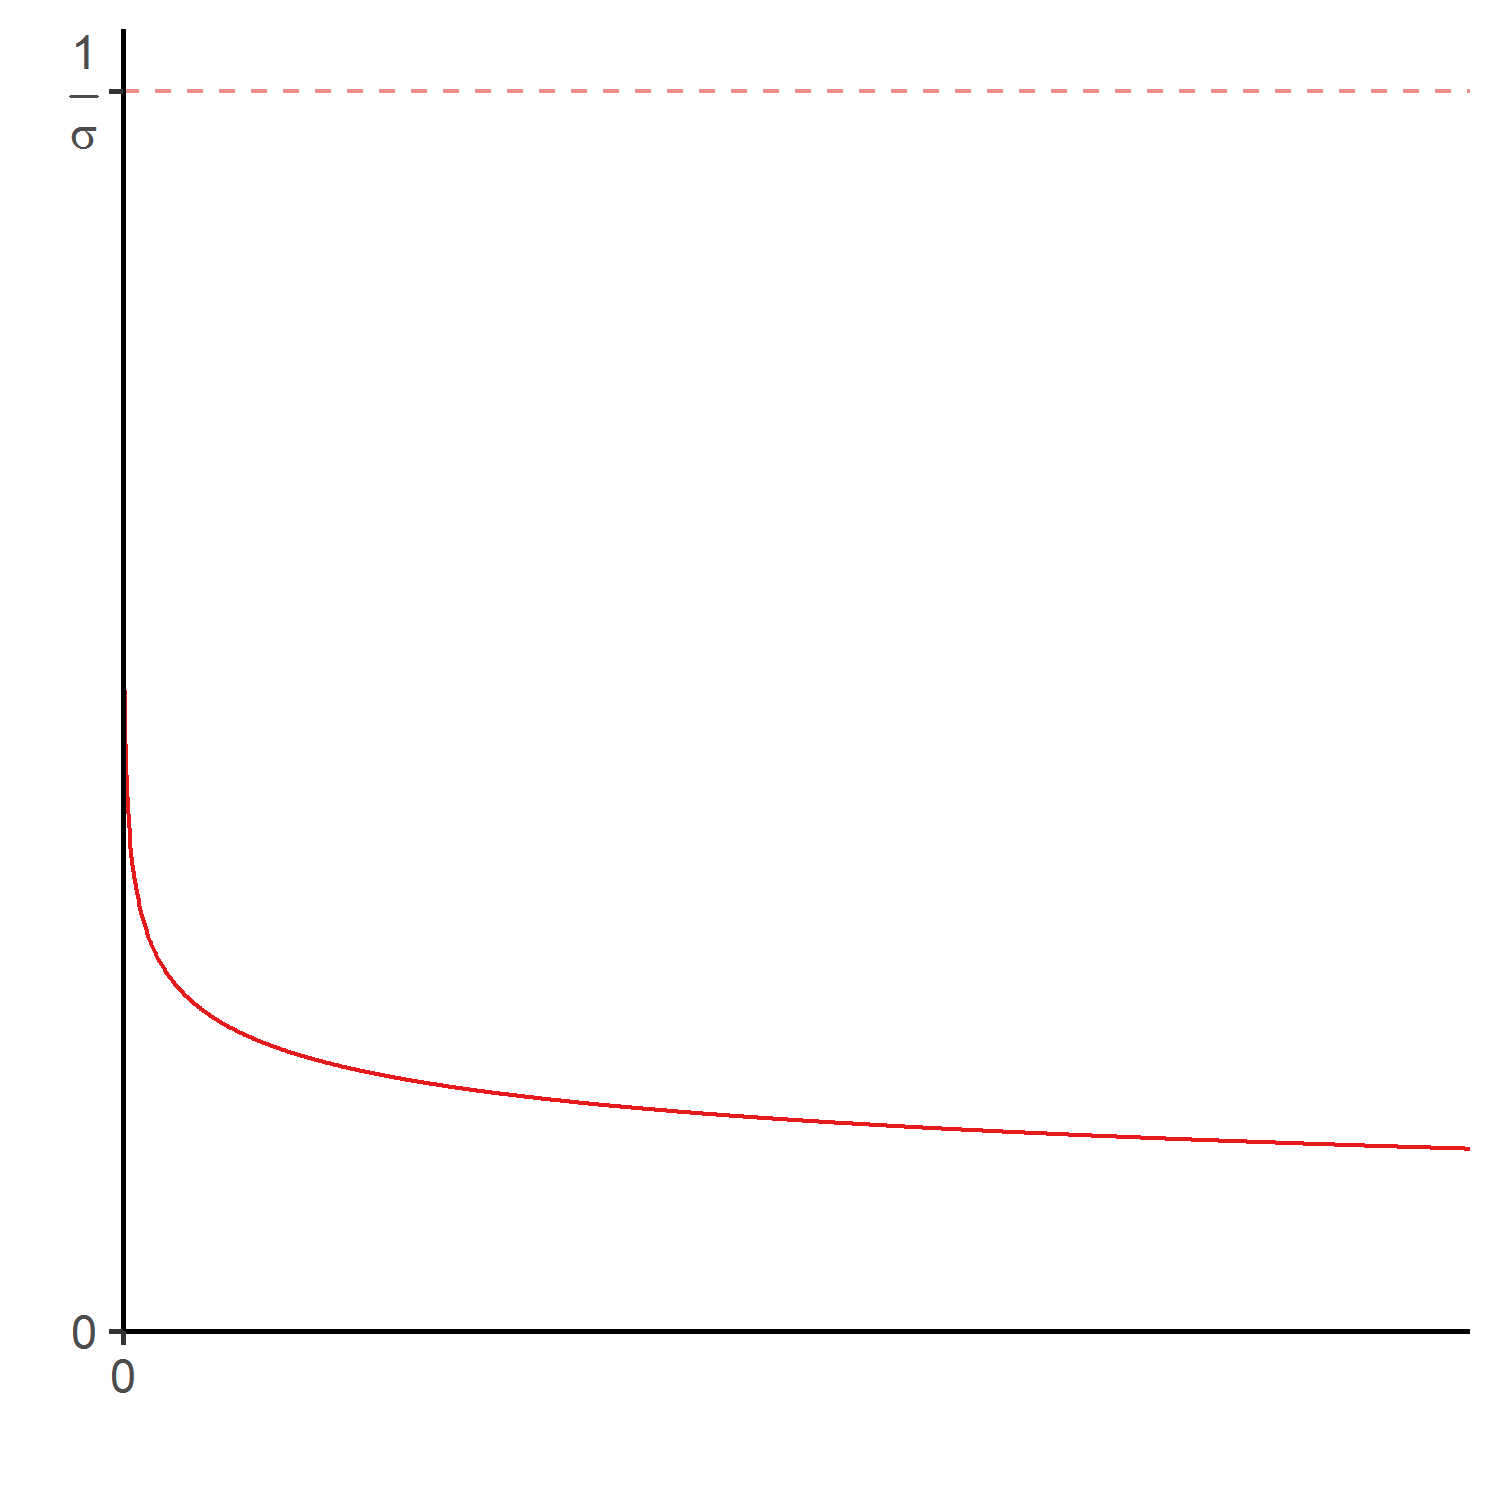
\includegraphics[width=1\linewidth]{../result/appendix_A/function_h/graph_2.png} 
		\caption{$\sigma \in \left(0.5, 1\right)$} 
		\label{fig:h_shape_2} 
	\end{subfigure}
	%%%
	\begin{subfigure}[t]{0.32\linewidth}
		\centering
		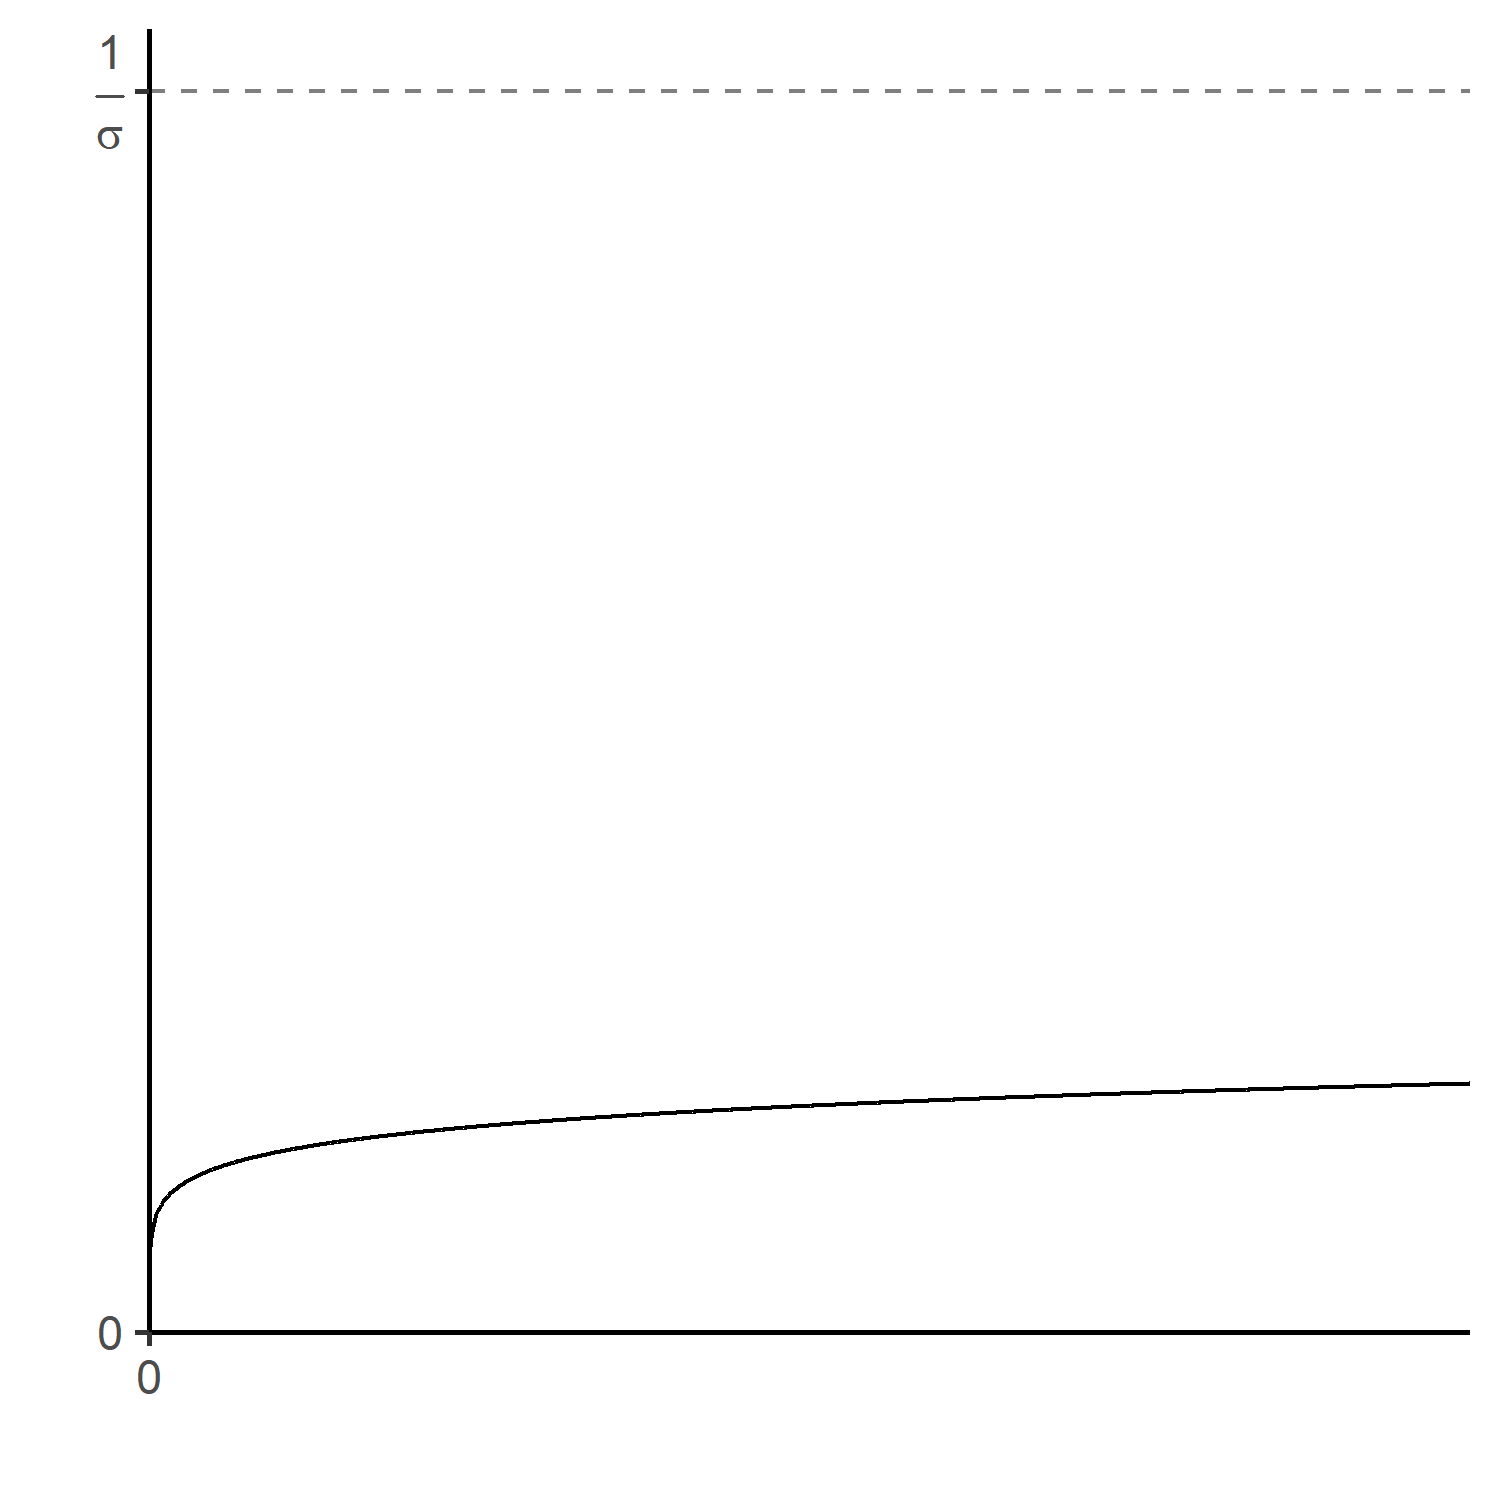
\includegraphics[width=1\linewidth]{../result/appendix_A/function_h/graph_3.png} 
		\caption{$\sigma > 1$} 
		\label{fig:h_shape_3} 
	\end{subfigure} 
	\caption{Different possible shapes of the $h$ function, according to the value of $\sigma$.}
	\label{fig:h_shape}
	\vspace{.5ex}
	\hrule
	\vspace{-4ex}
	\justify\singlespacing\footnotesize The x-axis corresponds to $k_t$. Scales are different according to the graph. The functions graphs are drawn using numerical computation with following set of parameters for each case:\\
	(a) $\sigma = 0.25$, $\phi = 0.3$, $\gamma = 0.5$ ; \hspace{4ex}(b) $\sigma = 0.8$, $\phi = 0.3$, $\gamma = 0.5$ ; \hspace{4ex}(c) $\sigma = 1.2$, $\phi = 0.3$, $\gamma = 0.5$.
\end{figure}

\begin{proposition}\label{prop:full_emp}
	If $k_t \leq k_1$ at the equilibrium, then:
	\begin{enumerate}[label=(\roman*)]
		\item there is a unique equilibrium with full employment where $k_t = k_1$,
		\item the net wage equals the unemployment benefits, i.e. $(1-\tau_t)w_t = b_t$.
	\end{enumerate} 
\end{proposition}
\begin{proof}
	The numerator of the $g$ function is positive if and only if $k_t > k_1 \Leftrightarrow L_t < N_t^y$ (i.e. the number of worker is smaller than the young population size). This condition is always satisfied when there is unemployment. However, if this condition is not satisfied, it would mean that the labor demand exceeds the labor force (i.e. $L_t^d > N_t^y$). Therefore, the economy should face full-employment (i.e. $L_t = N_t^y$) and the capital-per-worker at the equilibrium with full-employment is $k_t = k_1$. In such a case, $X_t$ would tend to  $-\infty$. However, the lower bound of $X_t$ is $0$. Because if $X_t$ is negative, the unemployment benefits would exceed the net wage. I consider that such a case is not possible.\footnote{Even though I consider a model with inelastic labor supply, no agent would work for a wage which is lower than unemployment benefits. This assumption can be considered as an incentive constraint.} Thus, if $k_t \leq k_1 \implies k_t = k_1 \implies u_t = 0 \implies X_t = 0 \implies (1-\tau_t)w_t = b_t$.
\end{proof}

Therefore, the equilibrium with unemployment requires $k_t > k_1$. Hence, any equilibrium in the case represented in figure \ref{fig:g_shape_b} leads to the equilibrium with full-employment.

I normalize $k_t$ to the vertical asymptote $k_1$. Let $\nu = k_2/k_1$ with $\nu > 0$. It implies that $k_2 \gtreqqless k_1$ when $\nu \gtreqqless 1$. Let $\tilde{k}_t = k_t / k_1$ with $\tilde{k}_t > 0$. As for $\nu$, if $\tilde{k}_t$ is greater than unity, then $k_t>k_1$ and vice-versa. To simplify the notation, let $\rho = \frac{\sigma-1}{\sigma} \in \left(-\infty, 1\right)$.\footnote{When both input factors are gross complement, the elasticity of substitution is $\sigma \in \left(0,1\right)$ and the corresponding interval for $\rho$ is $\left(-\infty, 0\right)$. However, when both are gross substitute, the elasticity of substitution is $\sigma \in \left(0,+\infty\right)$ and the corresponding interval for $\rho$ is $\left(0,1\right)$.} Using this specification, it is possible to rewrite $g$ such that:
\begin{equation*}
g(\tilde{k}_t; \nu, \rho) = \ln\left(\frac{\tilde{k}_t - 1}{\tilde{k}_t^\rho - \nu^\rho}\right) + \rho\ln\left(\nu\right)
\end{equation*}
Let also rewrite the $h$ function such that:
\begin{equation*}
h(\tilde{k}_t ; \tilde{\gamma}, \rho) = \left( \frac{1}{1-\rho} + \tilde{\gamma} \tilde{k}_t^{-\rho} \right)^{-1}
\end{equation*}
where $\tilde{\gamma} \equiv \frac{1-\phi}{\phi} \frac{1-\gamma(1-\sigma)}{\gamma} k_1^{-\rho}> 0$.

\subsection*{A.1 Under gross-complementarity, i.e. $\rho < 0$}

$g(\tilde{k}_t)$ is define and continuous between both vertical asymptotes within the logarithm, so $1$ and $\nu$.\footnote{These vertical asymptotes correspond to $k_1$ and $k_2$ before the normalization.} When $\nu$ is greater than unity, $g(\tilde{k}_t)$ is defined and continuous on $\left(1, \nu\right)$. While the function is defined and continuous on $\left(\nu, 1\right)$ when $\nu < 1$. Finally, when $\nu = 1$, $\tilde{k}_t$ can take a unique value which corresponds to $1$. This definition domain is due to the properties of the logarithm. Both parts of the product within the logarithm must have the same sign in order to remain defined. The $g$ function has two possible shapes according to the value of $\nu$ with respect to unity:
\begin{enumerate}
	\item if $\nu > 1$:
	\begin{enumerate}
		\item $g(\tilde{k}_t)$ is strictly increasing in $\tilde{k}_t$,% i.e. $\frac{\partial g}{\partial \tilde{k}_t} > 0$,
		\item $\lim_{\tilde{k}_t\to 1} g(\tilde{k}_t) = -\infty$  and $\lim_{\tilde{k}_t\to \nu} g(\tilde{k}_t) = +\infty$.
	\end{enumerate}
	\item if $\nu < 1$:
	\begin{enumerate}
		\item $g(\tilde{k}_t)$ is strictly decreasing in $\tilde{k}_t$,% i.e. $\frac{\partial g}{\partial \tilde{k}_t} < 0$,
		\item $\lim_{\tilde{k}_t\to 1} g(\tilde{k}_t) = +\infty$ and $\lim_{\tilde{k}_t\to \nu} g(\tilde{k}_t) = -\infty$.
	\end{enumerate}
\end{enumerate}
When $\rho<0$, the $h$ function is defined and continuous on $\mathbb{R}_+$ and has the following properties:
\begin{enumerate}
	\item $h(\tilde{k}_t)$ is strictly decreasing in $\tilde{k}_t$,% i.e. $\frac{\partial h}{\partial \tilde{k}_t} \leq 0$,
	\item $\lim_{\tilde{k}_t\to 0} h(\tilde{k}_t) = 1-\rho$ and $\lim_{\tilde{k}_t\to +\infty} h(\tilde{k}_t) = 0$.
\end{enumerate}

These properties leads to lemmas \ref{lemma:rho_lower0_nu_lower1} and \ref{lemma:rho_lower0_nu_higher1}. Using these intermediate results with proposition \ref{prop:full_emp}, I can prove proposition \ref{prop:full_emp}.
\begin{lemma}\label{lemma:rho_lower0_nu_lower1}
	if $\rho < 0$ and $\nu > 1$, then it exists a unique equilibrium.
\end{lemma}
\begin{proof}
	Let $\rho < 0$ and $\nu > 1$. The $g$ function is defined and continuous in $\tilde{k}_t \in \left(1, \nu \right)$, strictly increasing and has two infinite vertical asymptotes of opposite signs. The $h$ function is defined and continuous in $\tilde{k}_t \in \mathbb{R}_+ \supset \left(1, \nu \right)$, strictly decreasing and has two finite horizontal asymptotes $1/\sigma$ and $0$. Therefore, both functions intersect in only one point. Hence, there is uniqueness of the equilibrium.
\end{proof}
\begin{lemma}\label{lemma:rho_lower0_nu_higher1}
	if $\rho < 0$ and $\nu < 1$, then it exists at least one equilibrium.
\end{lemma}
\begin{proof}
	Let $\rho < 0$ and $\nu > 1$. The $g$ function is defined and continuous in $\tilde{k}_t \in \left(\nu, 1\right)$, strictly decreasing and has two infinite vertical asymptotes of opposite signs. The $h$ function is defined and continuous in $\tilde{k}_t \in \mathbb{R}_+ \supset \left(\nu, 1\right)$, strictly decreasing and has two finite horizontal asymptotes $1-\rho$ and $0$. Therefore, both functions intersect in at least one point. Hence, there is at least one equilibrium.
\end{proof}
\begin{proposition}
	if $\rho < 0$, then it exists a unique equilibrium.
\end{proposition}
\begin{proof}
	Lemma \ref{lemma:rho_lower0_nu_lower1} claims that there is a unique equilibrium when $\nu > 1$. There is also a unique equilibrium when $\nu = 1$. Lemma \ref{lemma:rho_lower0_nu_higher1} asserts that there is at least one equilibrium when $\nu < 1$. Yet, proposition \ref{prop:full_emp} states that any equilibrium when $\nu > 1$ leads to the unique equilibrium with full-employment. Therefore, if $\rho < 0$ there is a unique equilibrium.
\end{proof}

\subsection*{A.2 Under gross-substituability, i.e $0 < \rho < 1$}

Contrary to the previous case, $g(\tilde{k}_t)$ is defined and continuous on $\mathbb{R}_+$ but outside of both vertical asymptotes within the logarithm, so $1$ and $\nu$. When $\nu$ is greater than unity, $g(\tilde{k}_t)$ is defined and continuous on $(0, 1) \cap (\nu, +\infty)$. While the function is defined and continuous on $(0, \nu) \cap (1, +\infty)$ when $\nu < 1$. Finally, when $\nu = 1$, the function is defined and continuous on $\mathbb{R}_+$ but has no longer infinite discontinuity. Regardless of the value of $\nu$, $\lim_{\tilde{k}_t\to 0} = 0$ and $\lim_{\tilde{k}_t\to +\infty} = +\infty$. Both vertical asymptotes correspond to $\lim_{\tilde{k}_t\to 1} g(\tilde{k}_t) = -\infty$ and $\lim_{\tilde{k}_t\to \nu} g(\tilde{k}_t) = +\infty$. The $g$ function has two possible shapes according to the value of $\nu$ with respect to unity.\footnote{Excluding the case where $\nu=1$.} Moreover, $g(\tilde{k}_t)$ is strictly increasing in $\tilde{k}_t$ when $\nu < 1$. When $\rho > 1$, the $h$ function is defined and continuous on $\mathbb{R}_+$ and has the following properties:
\begin{enumerate}
	\item $h(\tilde{k}_t)$ is strictly increasing in $\tilde{k}_t$,
	\item $\lim_{\tilde{k}_t\to 0} h(\tilde{k}_t) = 0$ and $\lim_{\tilde{k}_t\to +\infty} h(\tilde{k}_t) = 1-\rho$.
\end{enumerate}
I plot both functions with numerical computation for feasible values of $\sigma$ according to the model conditions as detailed in section \ref{subsec:wage_bargaining}. The parameters $\gamma$ and $\phi$ are set according to the calibration in section \ref{subsec:calibration}, thus $\gamma = 0.5$ and $\phi = 0.3$.\footnote{The exact values for $\phi$ are 0.27 for France and 0.325 for the United-States. I use 0.3 for this numerical computation as an approximation of the mean.} Figure \ref{fig:gh2} shows both functions in the case where $\nu < 1$.
\begin{figure}[tb]
	\centering
	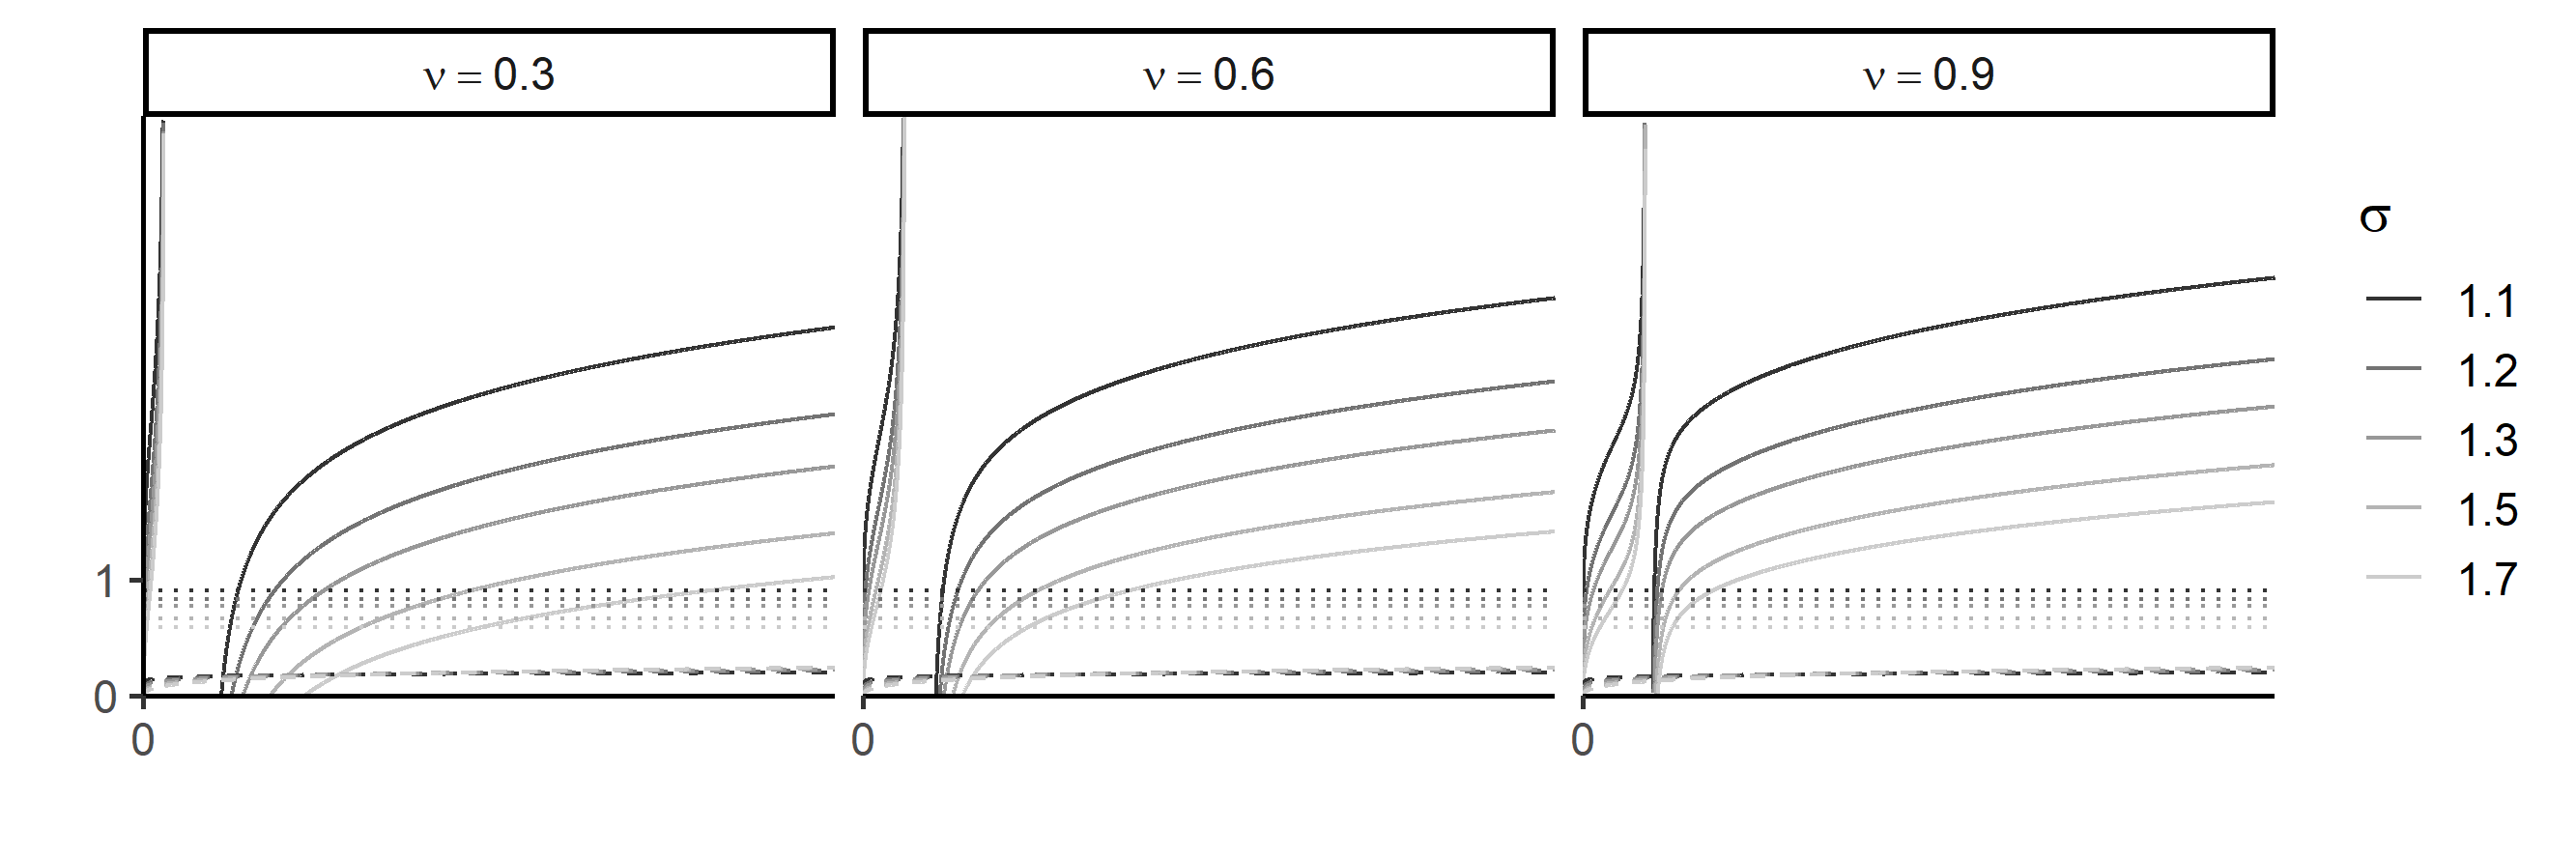
\includegraphics[width = 1\linewidth]{../result/appendix_A/uniqueness/gd_all.png}
	\caption{Numerical simulation of $g$ (solid line) and $h$ (dashed line), according to the values of $\sigma$ and $\nu$.}
	\label{fig:gh2}
	\vspace{.5ex}
	\hrule
	\vspace{-4ex}
	\justify\singlespacing\footnotesize The x-axis corresponds to $\tilde{k}_t$. The dotted lines correspond to $1-\rho$, so the infinite limit in $\tilde{k}_t$ of the $h$ function.
\end{figure}
Looking at the behavior of both functions, they do intersect in only one point beyond $1$. Therefore, I make the following conjecture:
\begin{conjecture}\label{conj:rho_higher0_nu_lower1}
	if $\rho \in (0,1)$ and $\nu < 1$, then it exists a unique equilibrium.
\end{conjecture}
This unique equilibrium is the one with unemployment since it lies beyond $1$ and therefore beyond $k_1$ without normalization. I also do the numerical computation in the case where $\nu > 1$, with the same values for $\gamma$ and $\phi$. Figure \ref{fig:gh1} plots the result.
\begin{figure}[tb]
	\centering
	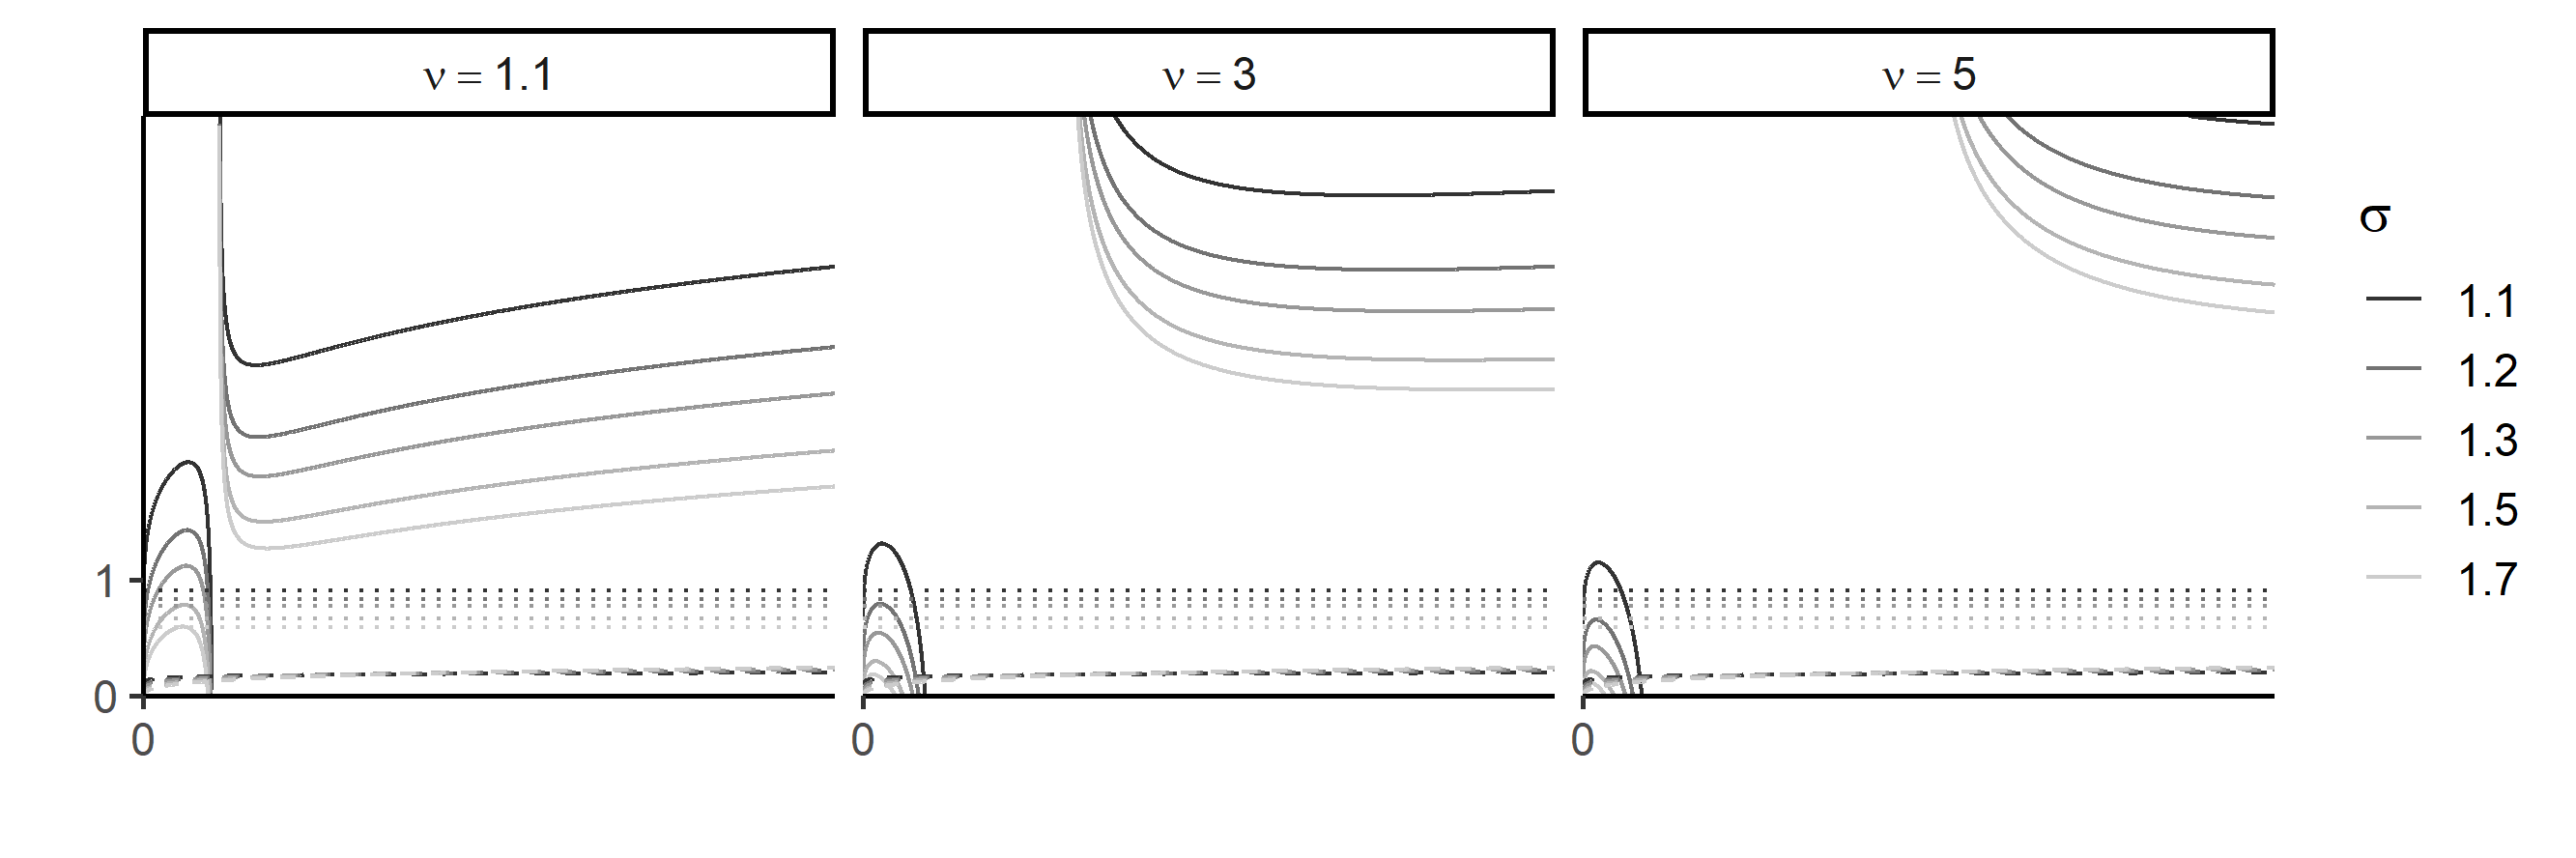
\includegraphics[width = 1\linewidth]{../result/appendix_A/uniqueness/gc_all.png}
	\caption{Numerical simulation of $g$ (solid line) and $h$ (dashed line), according to the values of $\sigma$ and $\nu$.}
	\label{fig:gh1}
	\vspace{.5ex}
	\hrule
	\vspace{-4ex}
	\justify\singlespacing\footnotesize The x-axis corresponds to $\tilde{k}_t$. The dotted lines correspond to $1-\rho$, so the infinite limit in $\tilde{k}_t$ of the $h$ function.
\end{figure}
Looking at the behavior of both functions, they do intersect two times before $1$. Therefore, I make the following conjecture:
\begin{conjecture}\label{conj:rho_higher0_nu_higher1}
	if $\rho \in (0,1)$ and $\nu > 1$, then it exists at least one equilibrium lying below unity.
\end{conjecture}
Using these two conjectures with proposition \ref{prop:full_emp}, I can prove that there is a unique equilibrium for all $\rho \in (0,1)$.\footnote{Except in the case where $\nu = 1$, i.e. $k_1 = k_2$. In such a case, the infinite discontinuity disappears and so does the equilibrium.}
\begin{proposition}
	if $\rho \in (0,1)$, then it exists a unique equilibrium.
\end{proposition}
\begin{proof}
	Conjecture \ref{conj:rho_higher0_nu_lower1} claims that there is a unique equilibrium when $\nu < 1$. Conjecture \ref{conj:rho_higher0_nu_higher1} asserts that there is at least one equilibrium when $\nu > 1$ lying below unity. Thus, there is at least one equilibrium such that $k_t < k_1$. Yet, proposition \ref{prop:full_emp} states that any equilibrium with $k_t \leq k_1$ leads to the unique equilibrium with full-employment. Therefore, if $\rho \in (0,1)$ there is a unique equilibrium.
\end{proof}




	
	\section*{Appendix B. Derivatives} \label{appendix:derivatives}
	\addcontentsline{toc}{section}{Appendix B. Derivatives}
	I derive the partial derivative of both functions $g$ and $h$ that determine the equilibrium.

\subsection*{B.1 The $g$ function's derivatives}

	\begin{equation*}
		g(L_t, K_t, \eta_t, N_t^y; \phi, \sigma) = 
		\ln\left[ \frac{ \frac{N_t^y}{L_t} - 1 } { \frac{\phi}{1-\phi} \left(\frac{K_t}{L_t}\right)^{\frac{\sigma-1}{\sigma}} \eta_t - 1 }\right]
	\end{equation*}
The partial derivative of the $g$ function with respect to $\eta_t$ is:
	\begin{equation*}
		g_\eta = - \frac{\frac{\phi}{1-\phi}k_t^{\frac{\sigma-1}{\sigma}}}{\frac{\phi}{1-\phi}k_t^{\frac{\sigma-1}{\sigma}}\eta_t - 1} = - \left(\eta_t - \Theta_t\right)^{-1} < 0
	\end{equation*}
where $\eta_t/\Theta_t - 1$ corresponds to the denominator within the logarithm of the $g$ function. At the equilibrium with unemployment, the denominator must be positive. Therefore $\eta_t - \Theta_t >0 \implies g_\eta < 0$. The partial derivative of the $g$ function with respect to $N_t^y$ is:
	\begin{equation*}
		g_{N^y} = \left(N_t^y-L_t\right)^{-1} > 0
	\end{equation*}
At the equilibrium with unemployment, the young population size exceeds the number of workers. Thus, $N_t^y-L_t > 0 \implies g_{N^y} > 0$. The partial derivative of the $g$ function with respect to $K_t$ is:
	\begin{align*}
		g_K &= -\frac{1}{K_t}\frac{\sigma - 1}{\sigma}\frac{\frac{\phi}{1-\phi}k_t^{\frac{\sigma-1}{\sigma}}\eta_t}{\frac{\phi}{1-\phi}k_t^{\frac{\sigma-1}{\sigma}}\eta_t - 1} \\
		g_K &= -\frac{1}{K_t}\frac{\sigma - 1}{\sigma}\left(1-\Theta_t/\eta_t\right)^{-1} \lessgtr 0,~\forall \sigma \gtrless 1
	\end{align*}
The sign of the derivative depends on the value of the elasticity of substitution between capital and labor with respect to 1. Finally, the partial derivative of the $g$ function with respect to $L_t$, after some simplifications, is:
	\begin{align*}
		g_L &= -\frac{1}{N_t^y-L_t} - \frac{1}{\sigma L_t} \left(\frac{\phi}{1-\phi}k_t^{\frac{\sigma-1}{\sigma}}\eta_t - \sigma\right) \\
		g_L &= -\frac{1}{N_t^y-L_t} - \frac{1}{\sigma L_t} \left(\eta_t/\Theta_t - \sigma\right)
	\end{align*}
At the equilibrium with unemployment, $\eta_t/\Theta_t > 1$. $\eta_t/\Theta_t -\sigma$ is always positive for $\sigma < 1$, thus $g_L < 0~\forall \sigma < 1$. However, the sign cannot be deduced without additional assumptions for $\sigma > 1$. A more restrictive condition is required, i.e. $\eta_t/\Theta_t > \sigma$. In such a case, the partial derivative is unambiguously negative. If this condition is not met, $g_L$ can still be negative provided that the unemployment rate is lower than a threshold $\bar{u}_t = \left(1 - \frac{\eta_t}{\Theta_t \sigma}\right)^{-1}$. Otherwise, $g_L$ is positive.

\subsection*{B.2 The $h$ function's derivatives}

	\begin{equation*}
		h(L_t, K_t; \sigma, \phi, \gamma) = \left[ \sigma + \frac{1-\phi}{\phi} \frac{1-\gamma(1-\sigma)}{\gamma} \left(\frac{K_t}{L_t}\right)^{\frac{1-\sigma}{\sigma}} \right]^{-1}
	\end{equation*}
The partial derivative of the $h$ function with respect to $K_t$ is:
	\begin{equation*}
		h_K = \frac{1}{K_t}\frac{\sigma-1}{\sigma}\frac{\frac{1-\phi}{\phi}\frac{1-\gamma(1-\sigma)}{\gamma}k_t^{\frac{1-\sigma}{\sigma}}}{\left(\sigma + \frac{1-\phi}{\phi}\frac{1-\gamma(1-\sigma)}{\gamma}k_t^{\frac{1-\sigma}{\sigma}}\right)^2} \gtrless 0,~\forall \sigma \gtrless 1
	\end{equation*}
The partial derivative of the $h$ function with respect to $L_t$ is:
	\begin{equation*}
		h_L = -\frac{1}{L_t}\frac{\sigma-1}{\sigma}\frac{\frac{1-\phi}{\phi}\frac{1-\gamma(1-\sigma)}{\gamma}k_t^{\frac{1-\sigma}{\sigma}}}{\left(\sigma + \frac{1-\phi}{\phi}\frac{1-\gamma(1-\sigma)}{\gamma}k_t^{\frac{1-\sigma}{\sigma}}\right)^2} \lessgtr 0,~\forall \sigma \gtrless 1
	\end{equation*}






	\section*{Appendix C. Estimation of $\sigma$} \label{appendix:sigma}
	\addcontentsline{toc}{section}{Appendix C. Estimation of $\sigma$}
	The CES production function with biased technical change as defined by \cite{David1965} is:
\begin{equation*}
	Y_t = A\left[\left(E_t^K K_t\right)^\frac{\sigma-1}{\sigma} + \left(E_t^L L_t\right)^\frac{\sigma-1}{\sigma}\right]^\frac{\sigma}{\sigma-1}
\end{equation*}
where $E_t^K$ and $E^L_t$ represent the efficiency levels of both input factors. I assume linear growth rates of efficiency levels, so $E_t^i = E_0^i e^{a_i(t-t_0)}$ where $a_i$ denotes growth in technical progress associated with factor $i \in \lbrace K,L \rbrace$ and represents a linear time trend. To normalize the production function, I follow the specification of \cite{Klump2007},
\begin{equation*}
	E_0^K = \frac{Y_0}{K_0}\left(\frac{1}{\phi_0}\right)^\frac{\sigma}{1-\sigma} ~~\text{and}~~
	E_0^L = \frac{Y_0}{L_0}\left(\frac{1}{1-\phi_0}\right)^\frac{\sigma}{1-\sigma}
\end{equation*}
Normalization of the CES production function requires that factor shares are not biased by the growth of factor efficiencies at the fixed point. At time $t = t_0$, $e^{a_i(t-t_0)} = 1$.  Thus, they are just equal to the initial distribution parameters $\phi_0$ and $1-\phi_0$. Assuming that the firm is on its labor demand curve, as in the model, the labor share at time $t$ is :
\begin{equation*}
	\theta_t \equiv \frac{w_t L_t}{Y_t} = \left[1 + \left(\frac{E_t^K}{E_t^L}\frac{K_t}{L_t}\right)^\frac{\sigma-1}{\sigma}\right]^{-1}
\end{equation*}
Substituting with both efficiency levels, the labor share becomes:
\begin{equation*}
	\theta_t = \left[1 + \frac{\phi_0}{1-\phi_0}\left(\frac{K_t}{K_0}\frac{L_0}{L_t} e^{(a_K-a_L)(t-t_0)} \right)^\frac{\sigma-1}{\sigma}\right]^{-1}
\end{equation*}
Let $k_t \equiv K_t/L_t$ the capital-to-labor ratio. Thus, the labor-to-capital income ratio is:
\begin{equation*}
	\Theta_t \equiv \frac{\theta_t}{1-\theta_t} = \frac{1-\phi_0}{\phi_0}\left(\frac{k_t}{k_0} e^{(a_K - a_L)(t-t_0)}\right)^{\frac{1-\sigma}{\sigma}}
\end{equation*}
Rewritting the above equation and taking logs,
\begin{equation} \label{eq:est_sigma}
	\ln \Theta_t = \alpha + \frac{1-\sigma}{\sigma} \ln \tilde{k}_t + \frac{1-\sigma}{\sigma}(a_K-a_L)\left(t-t_0\right)
\end{equation}
where $\tilde{k}_t$ is the normalized capital-to-labor ratio and $\alpha$ is constant.

With this form, it is not possible to identify each technical change growth rate (i.e. $a_K$ and $a_L$). However, it captures the overall bias in technical change (i.e. $a_K - a_L$). I estimate equation \eqref{eq:est_sigma} using OLS for France and United States over the period 1970-2010.\footnote{This is a single-equation estimation from the two first-order conditions of the profit maximization. As \cite{Klump2007} discussed, single-equation or two-equations estimations can be biased due to endogeneity. They recommend to use supply-side system estimation. However, the aim of this estimation is only to obtain a value to simulate the model. Therefore, the elasticity of substitution I obtain is the one within the model specification.} I use data and variables specifications as described in section \ref{subsec:calibration}. I consider four specifications. The first one is the RAW estimation, without biased technical change nor hours worked correction. Then, I only control for the average hours worked in the HWC estimation and for the biased technical change in the BTC estimation. Finally, both are used as control in the HWC-BTC estimation. Standard errors are relatively high due to the lack of observations. Equations are estimated by country with 41 observations for each one. When the coefficient associated to the line $\frac{1-\sigma}{\sigma}$ is not significant it means that the estimated elasticity is not statistically different from 1, i.e. the Cobb-Douglas case. Tables \ref{tab:sigma_est_fr} and \ref{tab:sigma_est_us} summarize the results for France and the United States, respectively.
% Sigma estimation for France
\begingroup
\renewcommand{\arraystretch}{1}
\begin{table}[tb]
	\caption{Estimation of the capital-labor elasticity of substitution ($\sigma$) for France (1970-2010)}\label{tab:sigma_est_fr}
	\centering
	\begin{threeparttable}
		\begin{tabular}{c D{.}{.}{-3} D{.}{.}{-3} D{.}{.}{-3} D{.}{.}{-3}}
			& \multicolumn{1}{c}{RAW} & \multicolumn{1}{c}{HWC} & \multicolumn{1}{c}{BTC} & \multicolumn{1}{c}{HWC-BTC} \\ \hline \hline \\ [-1ex]
			$\alpha$ 							& 1.130^{***} 	& 1.123^{***}	& 1.081^{***}	& 1.079^{***}	\\
												& (0.027)		& (0.027)		& (0.035)		& (0.033)		\\
			$\frac{1-\sigma}{\sigma}$ 			& -0.614^{***} 	& -0.470^{***}	& -0.273		& -0.218^{*}	\\
												& (0.045)		& (0.033)		& (0.165)		& (0.125)		\\
			$\frac{1-\sigma}{\sigma}(a_K-a_L)$ 	& 				&				& -0.007^{**}	& -0.007^{**}	\\
												& 				&				& (0.003)		& (0.003)		\\ [1ex] \hline \\ [-1ex]
			Biased technical change 			& \multicolumn{1}{c}{No} & \multicolumn{1}{c}{No} & \multicolumn{1}{c}{Yes} & \multicolumn{1}{c}{Yes} \\
			Hours worked correction 			& \multicolumn{1}{c}{No} & \multicolumn{1}{c}{Yes} & \multicolumn{1}{c}{No} & \multicolumn{1}{c}{Yes} \\ [1ex] \hline \\ [-1ex]		
			$\sigma$ 							& 2.593			& 1.887			& 1.375			& 1.279		\\ [1ex] \hline \hline
		\end{tabular}
%		\vspace{-3ex}
		\begin{tablenotes}
		{\footnotesize 
			\item \textit{Note :} $^{*}$p$<$0.1; $^{**}$p$<$0.05; $^{***}$p$<$0.01. Robust standard errors in parentheses.
		}
		\end{tablenotes}
	\end{threeparttable}
\end{table}
\endgroup
For France, worked hours seems to play a role in the estimation of the elasticity when I compare RAW to HWC. Not considering the hours worked correction may bias the elasticity of substitution toward relatively high values (2.593 against 1.887). I compare RAW to BTC and conclude that biased technical change has also to be taken into account. Even though the $\sigma$ associated coefficient is not significant, the biased technical change's coefficient is significant. Finally, controlling for both in HWC-BTC leads to an elasticity about 1.279. But it is only significant at a 90 \% confidence level. This is the result of a break in the regime as explained in \hyperref[appendix:regime]{appendix D}. The biased technical change coefficient is also significant as in BTC. It indicates that biased technical change has to be jointly considered with the hours worked for France.

For the United States, hours worked correction does matter by comparing RAW to HWC. Once I control for it, the elasticity of substitution is about 1.234. However, the technical change does not seem to be biased since both associated coefficients in BTC and HWC-BTC are not significant. The coefficient associated to the elasticity are below unity but not statistically significant. Thus, controlling for biased technical change is not necessary for the United States. I only have to control for average worked hours.
% Sigma estimation for US
\begingroup
\renewcommand{\arraystretch}{1}
\begin{table}[tb]
	\caption{Estimation of the capital-labor elasticity of substitution ($\sigma$) for the United States (1970-2010)}\label{tab:sigma_est_us}
	\centering
	\begin{threeparttable}
		\begin{tabular}{c D{.}{.}{-3} D{.}{.}{-3} D{.}{.}{-3} D{.}{.}{-3}}
			& \multicolumn{1}{c}{RAW} & \multicolumn{1}{c}{HWC} & \multicolumn{1}{c}{BTC} & \multicolumn{1}{c}{HWC-BTC} \\ \hline \hline \\ [-1ex]
			$\alpha$ 							& 0.636^{***}	& 0.648^{***}	& 0.643^{***}	& 0.649^{***} \\
												& (0.020)		& (0.022)		& (0.022)		& (0.021) \\
			$\frac{1-\sigma}{\sigma}$ 			& -0.177^{**}	& -0.189^{***}	& 0.155			& -0.647^{*} \\
												& (0.073)		& (0.067)		& (0.473)		& (0.348) \\
			$\frac{1-\sigma}{\sigma}(a_K-a_L)$ 	&				&				& -0.004		& 0.006 \\
												&				&				& (0.006)		& (0.005) \\ [1ex] \hline \\ [-1ex]
			Biased technical change 			& \multicolumn{1}{c}{No} & \multicolumn{1}{c}{No} & \multicolumn{1}{c}{Yes} & \multicolumn{1}{c}{Yes} \\
			Hours worked correction 			& \multicolumn{1}{c}{No} & \multicolumn{1}{c}{Yes} & \multicolumn{1}{c}{No} & \multicolumn{1}{c}{Yes} \\ [1ex] \hline \\ [-1ex]		
			$\sigma$ 							& 1.215			& 1.234			& 0.866			& 2.835 \\ [1ex]
			\hline \hline
		\end{tabular}
		\begin{tablenotes}
			{\footnotesize 
				\item \textit{Note :} $^{*}$p$<$0.1; $^{**}$p$<$0.05; $^{***}$p$<$0.01. Robust standard errors in parentheses.
			}
		\end{tablenotes}
	\end{threeparttable}
\end{table}
\endgroup
Therefore, I consider a capital-labor elasticity of substitution about 1.279 for France and 1.234 for the United States. These $\sigma$ values are used to compute the deduced parameter values (i.e. $\omega$ and $\beta$) in section \ref{subsec:calibration}.









	
	\section*{Appendix D. Two $\sigma$ regimes in France} \label{appendix:regime}
	\addcontentsline{toc}{section}{Appendix D. Two $\sigma$ regimes in France}
	Considering the estimation methodology in \hyperref[appendix:sigma]{appendix C}, I obtain a capital-labor elasticity of substitution around 1.279 for France over the period 1970-2010. However, the estimated coefficient is only significant at a 90\% confidence level. Such a result may be due to a break in the regime of $\sigma$. The relationship between the labor-to-capital income ratio $\Theta_t$ and the capital-per-worker $k_t$ depends on the value of $\sigma$ with respect to unity. From the comparatives statics derived in section \ref{sec:model}, it can be shown that :
	\begin{equation*}
		\frac{\partial \Theta_t}{\partial k_t} \gtreqqless 0 ~~ \text{when} ~~ \sigma \lesseqqgtr 1
	\end{equation*}
When both input factors are gross complement (i.e. $\sigma < 1$), the labor-to-capital income ratio and the capital-per-worker vary in the same direction. While they vary in opposite ways under gross substituability. The elasticity of substitution $\sigma$ is estimated using the following equation :
	\begin{equation*}
	\ln \Theta_t = \alpha + \frac{1-\sigma}{\sigma} \ln \tilde{k}_t + \frac{1-\sigma}{\sigma}(a_K-a_L)\left(t-t_0\right)
	\end{equation*}
Inspecting the time series of $\ln \Theta_t$ and $\ln \tilde{k}_t$, I suspect that there is a change of regime in the link between them. Figure \ref{fig:k_Theta_log} plots these time series.
	\begin{figure}[tb]
		\centering
		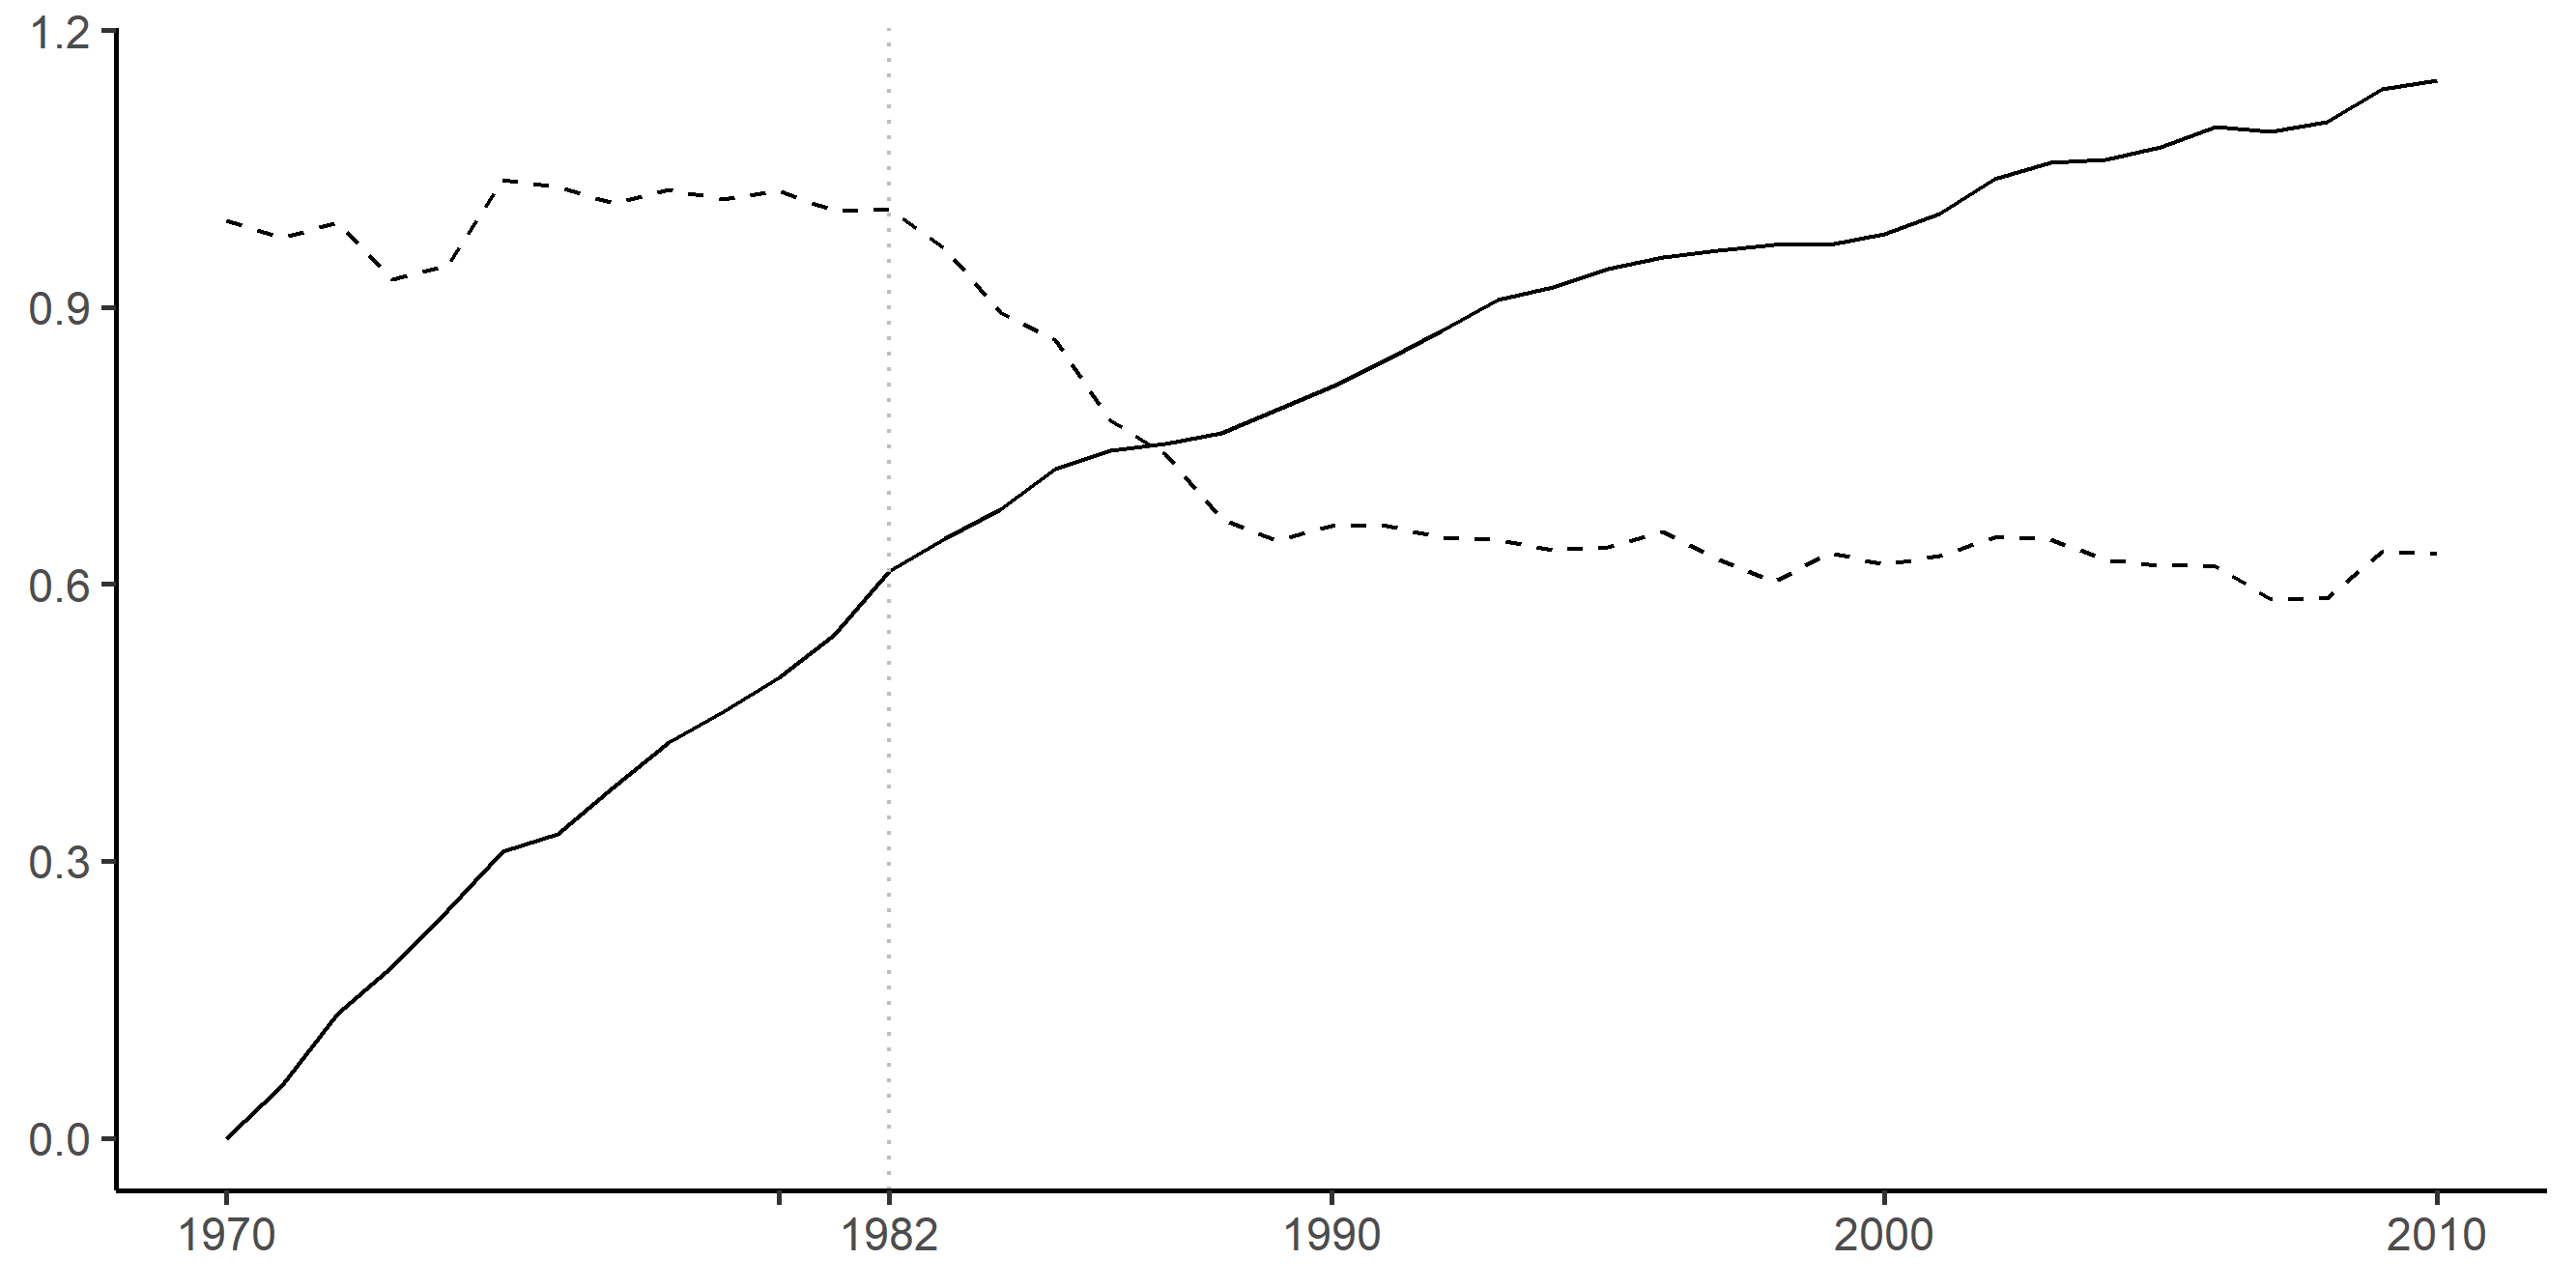
\includegraphics[width=1\linewidth]{../result/appendix_CD/k_Theta_log.png}
		\caption{$\ln \tilde{k}_t$ (solid) and $\ln \Theta_t$ (dashed) for France over the period 1970-2010}
		\label{fig:k_Theta_log}
	\end{figure}
The figure suggests that the correlation between both variables is different before and after the beginning of the 80's. Suppose that the change of regime in the relationship has occurred in 1982. The correlation between both variables is about 0.305 before 1982 and -0.787 after.\footnote{The year 1982 is included in the first sub-sample. Including it in the sub-sample after the break leads to the correlations of 0.499 and -0.786 for before and after respectively.} Such a difference in the correlation suggests that there are two regimes. However, the biased technical change has not been considered so far. Therefore, I have to detrend both variables in order to check whether the regime change is not driven by it. Using the Frisch-Waugh-Lovell theorem, I regress each variable on a linear time trend and extract the residuals as detrended variables. Both regressions correspond to the following:
	\begin{align*}
		\ln \Theta_t &= \varphi_0^\Theta + \varphi_1^\Theta \times t + \varepsilon_t^\Theta \\
		\ln \tilde{k}_t &= \varphi_0^{\tilde{k}} + \varphi_1^{\tilde{k}} \times t + \varepsilon_t^{\tilde{k}}
	\end{align*}
Figure \ref{fig:k_Theta_log_detrend} displays both detrended variables $\varepsilon_t^{\tilde{k}}$ and $\varepsilon_t^\Theta$. The vertical dashed lines correspond to potential break years in the regime. Looking at the variables behavior before and after the three thresholds, it suggests that there are still two regimes. Therefore, this result remains even when controlling for linear biased technical change.
	\begin{figure}[tb]
		\centering
		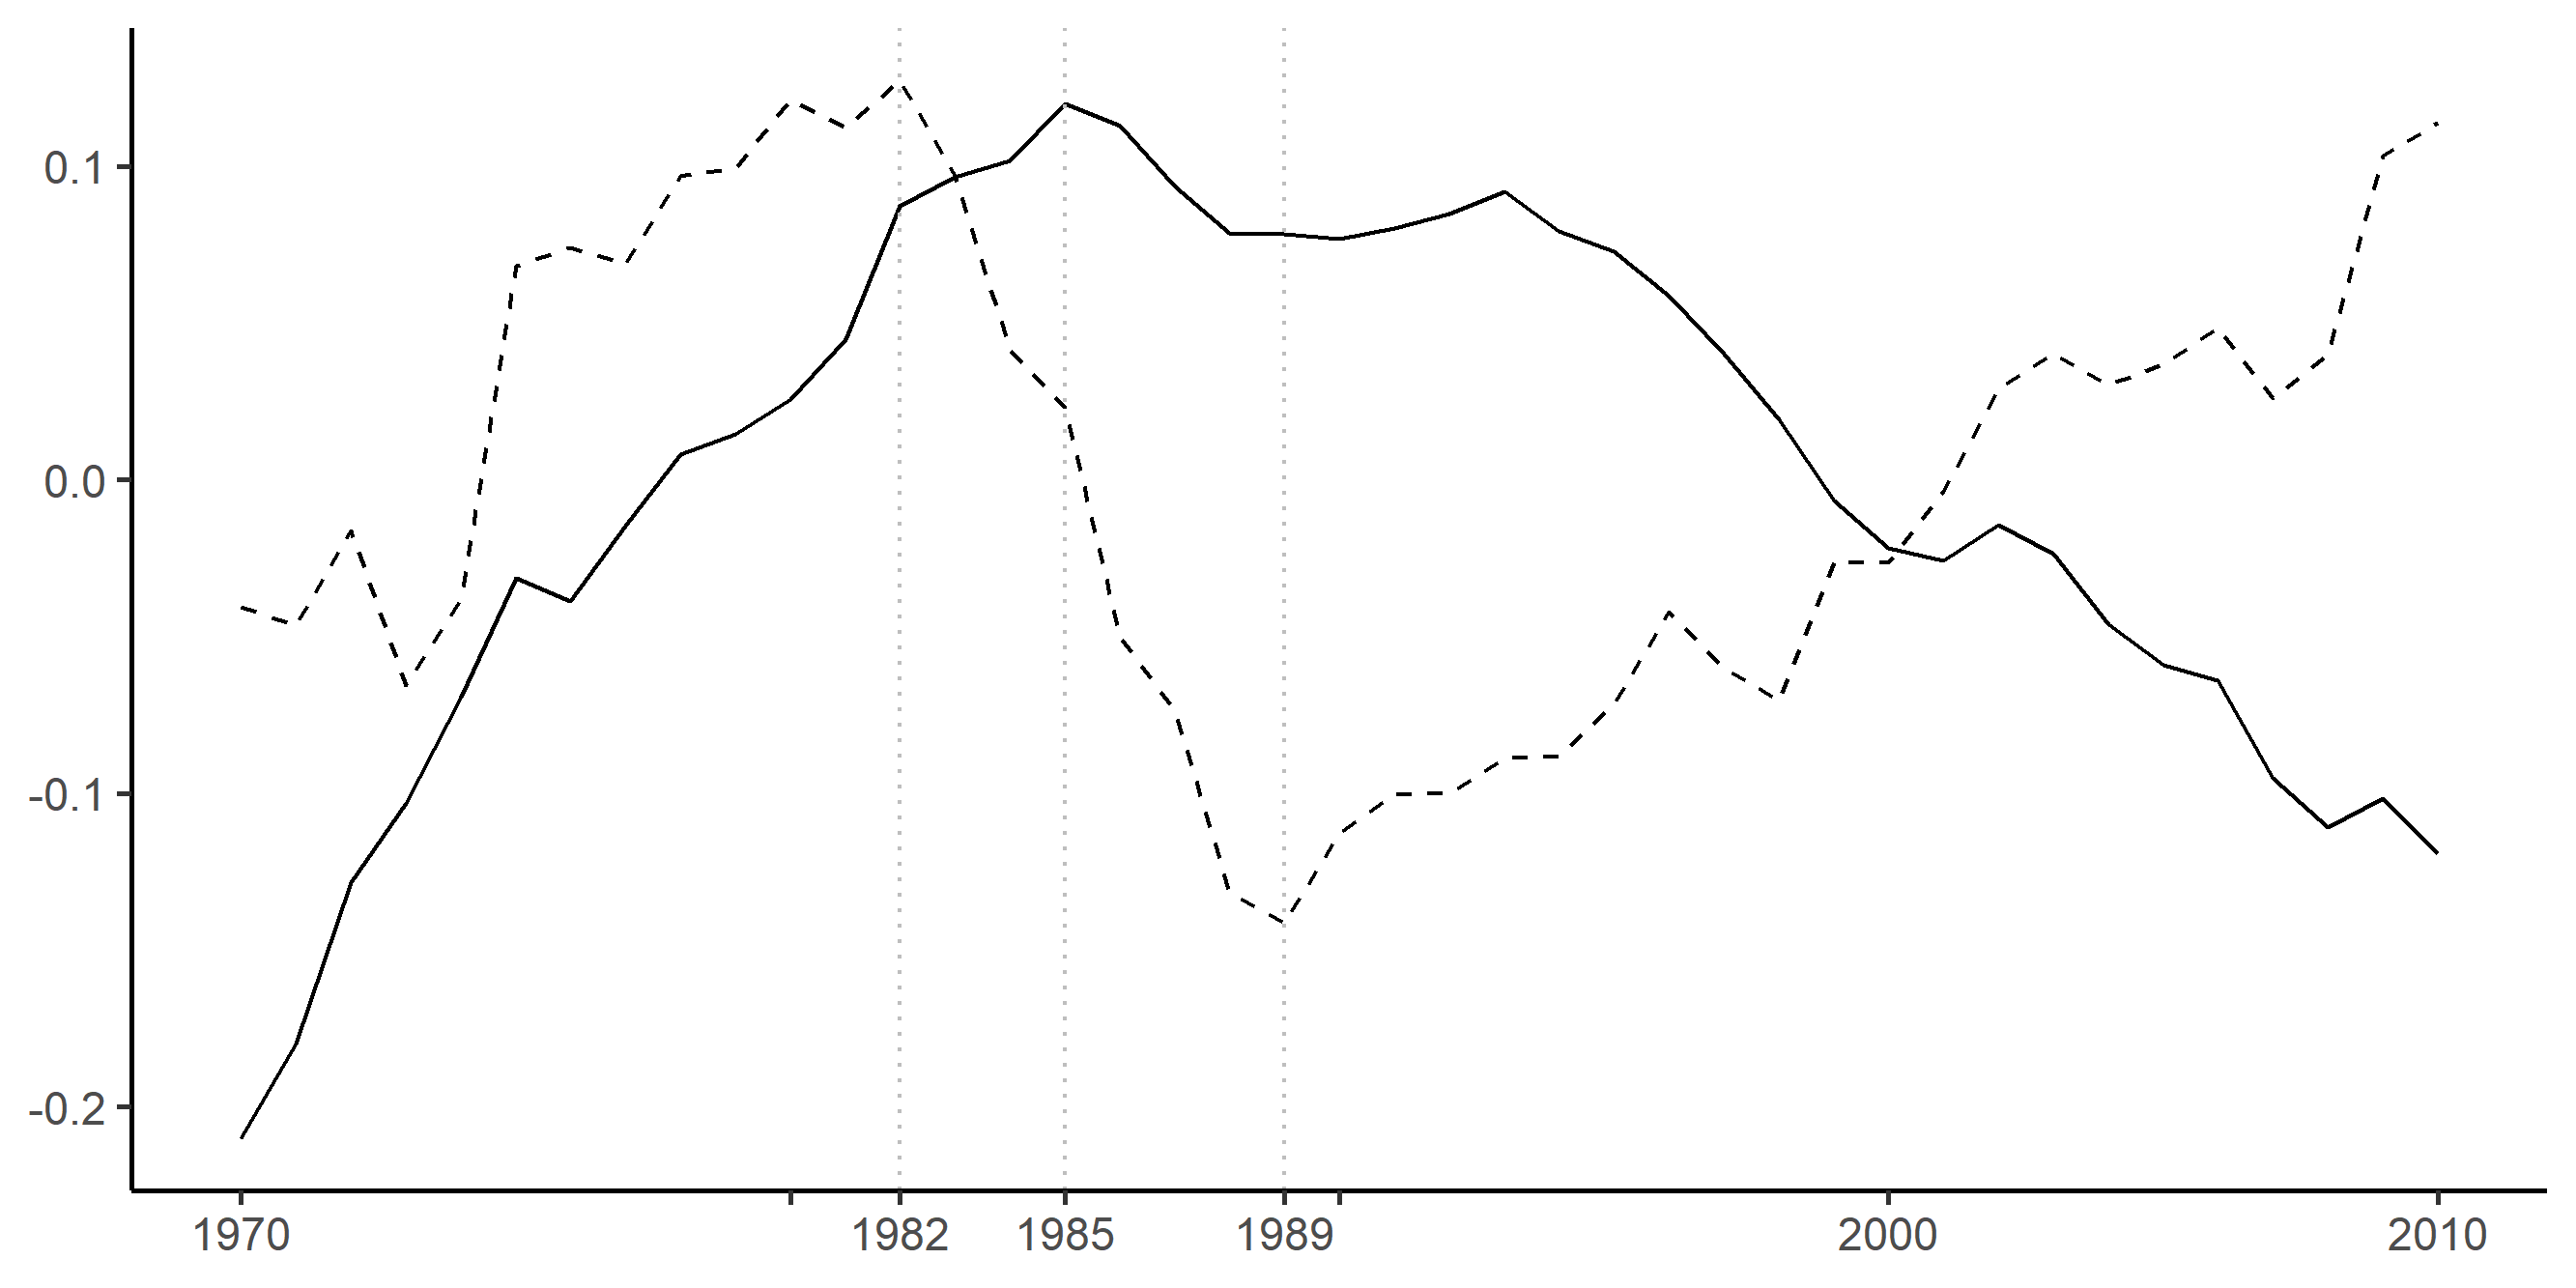
\includegraphics[width=1\linewidth]{../result/appendix_CD/k_Theta_log_detrend.png}
		\caption{$\varepsilon_t^{\tilde{k}}$ (solid) and $\varepsilon_t^\Theta$ (dashed) for France over the period 1970-2010}
		\label{fig:k_Theta_log_detrend}
	\end{figure}

For instance, figure \ref{fig:k_Theta_log_reg85} plots the regression lines before and after an elasticity regime change in 1985. The slope is positive between 1970 and 1985, so the elasticity would be smaller than 1 during this period and greater thereafter. All years between 1980 and 1990 are candidate to be the break year.
	\begin{figure}[tb]
		\centering
		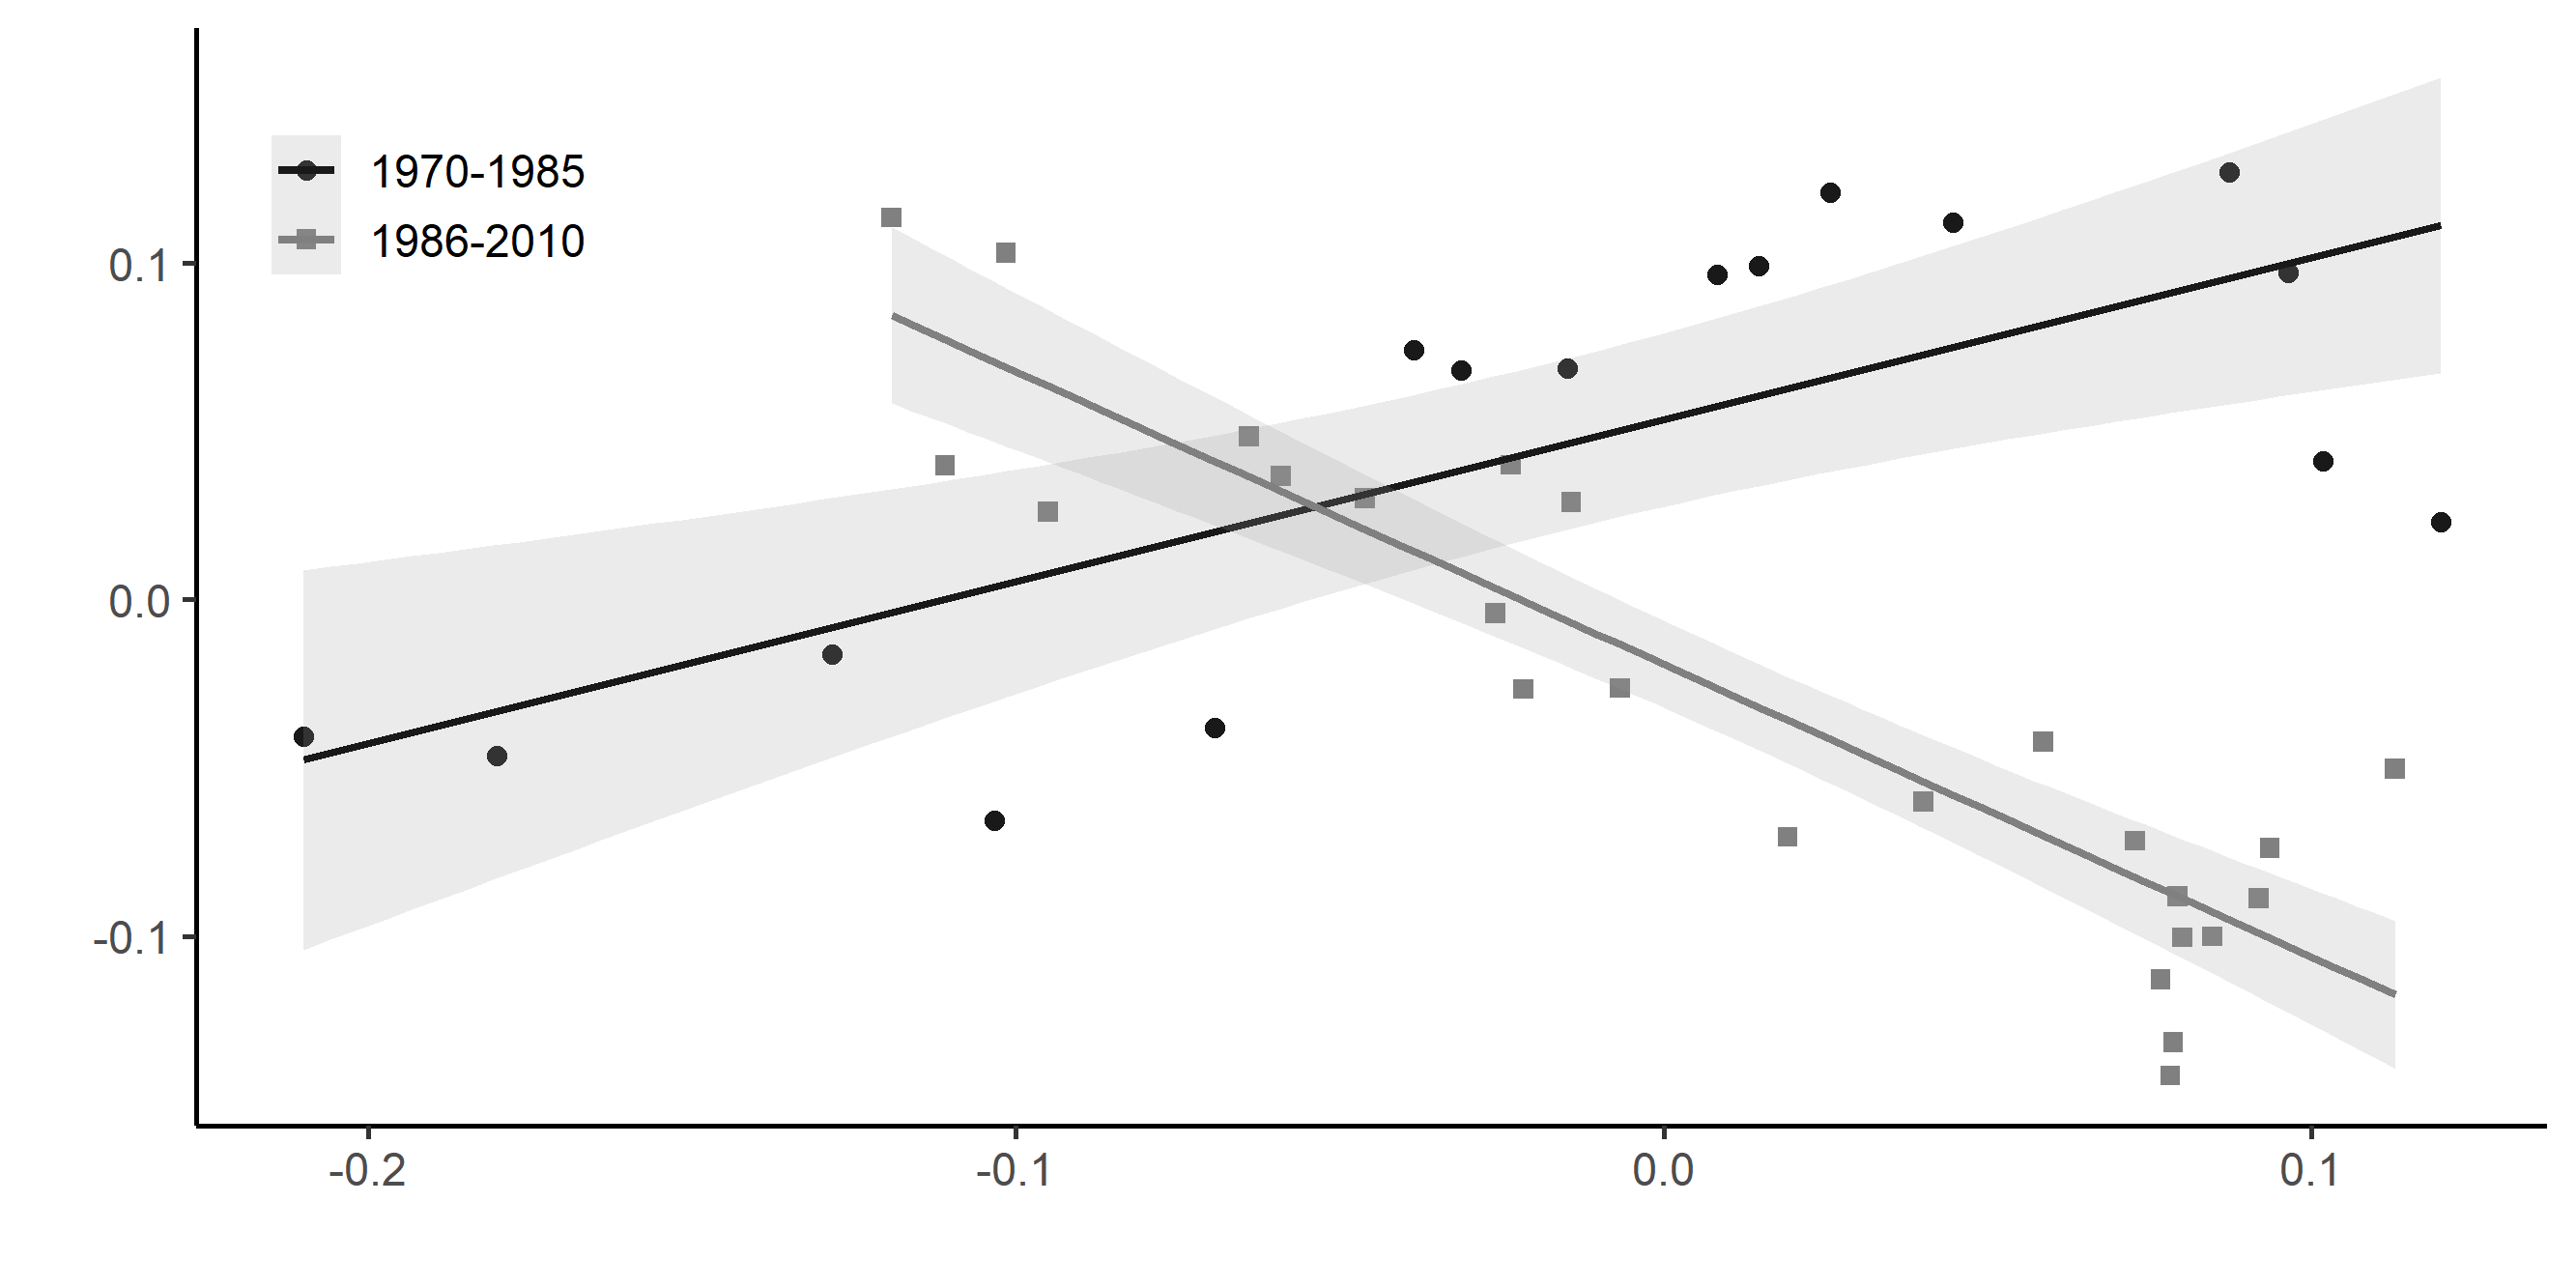
\includegraphics[width=1\linewidth]{../result/appendix_CD/k_Theta_log_reg85.png}
		\caption{Relationship between $\varepsilon_t^{\tilde{k}}$ (x-axis) and $\varepsilon_t^\Theta$ (y-axis) for France over the period 1970-2010}
		\label{fig:k_Theta_log_reg85}
		\vspace{.5ex}
		\hrule
		\vspace{-4ex}
		\justify\singlespacing\footnotesize The gray area corresponds to the confidence interval of the associated regression. The level of the confidence interval is set to 0.95.
	\end{figure}

To find which year corresponds to the most efficient break year, I run multiple regressions by changing the break year $\bar{t}$ for each regression. The estimated equation is:
	\begin{equation*}
		\varepsilon_t^{\Theta} = \nu_1 \mathds{1}_{\lbrace t \leq \bar{t} \rbrace} + \nu_2 \mathds{1}_{\lbrace t > \bar{t} \rbrace} + \rho_1 \mathds{1}_{\lbrace t \leq \bar{t} \rbrace} \varepsilon_t^{\tilde{k}} + \rho_2 \mathds{1}_{\lbrace t > \bar{t} \rbrace} \varepsilon_t^{\tilde{k}} + \zeta_t
	\end{equation*}
where $\mathds{1}$ is a dummy variable which is equal to 1 when the condition under brackets is satisfied, 0 otherwise. Table \ref{tab:break} displays the four coefficients (i.e. $\nu_1$, $\nu_2$, $\rho_1$, $\rho_2$) and the $R^2$ of each regression. The regression with a change in the regime in 1985 (i.e. $\bar{t} = 1985$) has the greatest $R^2$ and all its coefficients are significant. Thus, I assume that the break in the regime has occurred in 1985.
% Table break
\begingroup
\renewcommand{\arraystretch}{1}
\begin{table}[tb]
	\caption{Estimation of the capital-labor elasticity of substitution for France with break year}\label{tab:break}
	\centering
	\begin{threeparttable}
		\begin{tabular}{c D{.}{.}{-3} D{.}{.}{-3} D{.}{.}{-3} D{.}{.}{-3} D{.}{.}{-3}}
			$\bar{t}$ 	& \multicolumn{1}{c}{$\nu_1$} & \multicolumn{1}{c}{$\nu_2$} & \multicolumn{1}{c}{$\rho_1$} & \multicolumn{1}{c}{$\rho_2$} & \multicolumn{1}{c}{$R^2$} \\ \hline \hline \\ [-1ex]
	%		1974		& -0.044 		& 0.017 		& -0.017 		& -0.564^{***} 	& 0.264 \\
	%					& (0.090)		& (0.012)		& (0.610)		& (0.168)		& \\
	%		1975		& 0.028			& 0.015			& 0.424			& -0.554^{***}	& 0.244 \\
	%					& (0.090)		& (0.012)		& (0.610)		& (0.168)		& \\
	%		1976		& 0.054			& 0.014			& 0.580			& -0.540^{***}	& 0.239 \\
	%					& (0.053)		& (0.013)		& (0.421)		& (0.174)		& \\
	%		1977		& 0.062			& 0.012			& 0.634^{*}		& -0.529^{***}	& 0.247 \\
	%					& (0.044)		& (0.013)		& (0.371)		& (0.174)		& \\
	%		1978		& 0.070^{*}		& 0.009			& 0.694^{**}	& -0.520^{***}	& 0.278 \\
	%					& (0.036)		& (0.013)		& (0.322)		& (0.171)		& \\
	%		1979		& 0.075^{**}	& 0.006			& 0.725^{**}	& -0.514^{***}	& 0.317 \\
	%					& (0.030)		& (0.013)		& (0.286)		& (0.166)		& \\
			1980		& 0.080^{***}	& 0.002			& 0.765^{***}	& -0.516^{***}	& 0.385 \\
						& (0.025)		& (0.012)		& (0.251)		& (0.158)		& \\
			1981		& 0.079^{***}	& -0.002		& 0.762^{***}	& -0.533^{***}	& 0.461 \\
						& (0.021)		& (0.012)		& (0.217)		& (0.148)		& \\
			1982		& 0.077^{***}	& -0.007		& 0.736^{***}	& -0.607^{***}	& 0.596 \\
						& (0.016)		& (0.010)		& (0.168)		& (0.130)		& \\
			1983		& 0.071^{***}	& -0.012		& 0.677^{***}	& -0.690^{***}	& 0.705 \\
						& (0.013)		& (0.009)		& (0.131)		& (0.113)		& \\
			1984		& 0.062^{***}	& -0.015^{*}	& 0.580^{***}	& -0.764^{***}	& 0.741 \\
						& (0.011)		& (0.008)		& (0.114)		& (0.108)		& \\
			1985		& 0.053^{***}	& -0.019^{**}	& 0.482^{***}	& -0.870^{***}	& 0.780 \\
						& (0.010)		& (0.008)		& (0.098)		& (0.104)		& \\
			1986		& 0.043^{***}	& -0.022^{**}	& 0.365^{***}	& -0.928^{***}	& 0.713 \\
						& (0.011)		& (0.009)		& (0.106)		& (0.124)		& \\
			1987		& 0.034^{***}	& -0.023^{**}	& 0.282^{**}	& -0.956^{***}	& 0.635 \\
						& (0.012)		& (0.010)		& (0.116)		& (0.145)		& \\
			1988		& 0.024^{*}		& -0.022^{*}	& 0.202			& -0.931^{***}	& 0.507 \\
						& (0.013)		& (0.012)		& (0.133)		& (0.173)		& \\
			1989		& 0.016			& -0.019		& 0.131			& -0.893^{***}	& 0.391 \\
						& (0.014)		& (0.014)		& (0.145)		& (0.198)		& \\
			1990		& 0.009			& -0.018		& 0.082			& -0.871^{***}	& 0.321 \\
						& (0.015)		& (0.015)		& (0.151)		& (0.216)		& \\
			\hline \hline
		\end{tabular}
		\begin{tablenotes}
		{\footnotesize 
			\item \textit{Note :} $^{*}$p$<$0.1; $^{**}$p$<$0.05; $^{***}$p$<$0.01. Standard errors in parentheses.
		}
		\end{tablenotes}
	\end{threeparttable}
\end{table}
\endgroup
I have to estimate a value of $\sigma$ for 1970-1985 and another one for 1986-2010. I estimate the equation \eqref{eq:est_sigma} for each sub-sample with and without biased technical change. Table \ref{tab:sigma_sub} summarizes the results. 
% Table sigma
	\begingroup
\renewcommand{\arraystretch}{1}
\begin{table}[tb]
	\caption{Estimation of the capital-labor elasticity of substitution ($\sigma$) for France with break in the regime in 1986.}\label{tab:sigma_sub}
	\centering
	\begin{threeparttable}
		\begin{tabular}{c D{.}{.}{-3} D{.}{.}{-3} D{.}{.}{-3} D{.}{.}{-3}}
			Sample & \multicolumn{2}{c}{1970-1985} & \multicolumn{2}{c}{1986-2010} \\ \hline \hline \\ [-1ex]
			$\alpha$ 							& 1.007^{***} 	& 0.970^{***}	& 0.877^{***}	& 0.916^{***}	\\
												& (0.026)		& (0.040)		& (0.046)		& (0.160)		\\
			$\frac{1-\sigma}{\sigma}$ 			& -0.062	 	& 1.002			& -0.243^{***}	& -0.322 		\\
												& (0.059)		& (0.648)		& (0.048)		& (0.321)			\\
			$\frac{1-\sigma}{\sigma}(a_K-a_L)$ 	& 				& -0.050		&				& 0.001	\\
												& 				& (0.031)		& 				& (0.005)		\\ [1ex] \hline \\ [-1ex]
			Hours worked correction 			& \multicolumn{1}{c}{Yes} 	& \multicolumn{1}{c}{Yes} & \multicolumn{1}{c}{Yes} & \multicolumn{1}{c}{Yes} \\
			Biased technical change 			& \multicolumn{1}{c}{No} 	& \multicolumn{1}{c}{Yes} & \multicolumn{1}{c}{No} & \multicolumn{1}{c}{Yes} \\ [1ex] \hline \\ [-1ex]		
			$\sigma$ 							& 1.067			& 0.499			& 1.321			& 1.476		\\ [1ex]
			\hline \hline
		\end{tabular}
		\begin{tablenotes}
		{\footnotesize 
			\item \textit{Note :} $^{*}$p$<$0.1; $^{**}$p$<$0.05; $^{***}$p$<$0.01. Standard errors in parentheses.
		}
		\end{tablenotes}
	\end{threeparttable}
\end{table}
\endgroup
Biased technical change coefficients are not significant in both sub-sample regressions, neither are the coefficients associated to the elasticity. Therefore, I take into account the estimate where the technical change is not biased. Between 1970 and 1985, I set the capital-labor elasticity of substitution to unity, since the coefficient is not statistically different from 0.\footnote{This is mainly due to the lack of observations. The sub-sample has only 16 observations and therefore 14 degrees of freedom.} However, it is significant between 1986 and 2010 and the elasticity is about 1.321.
	
	
\end{document}